%%%%%%%%%%%%%%%%%%%%%%%%%%%%%%%%%%%%%%%%%%%%%%%%%%%%%%%%%%%%%%%%%%%
%                                                                 %
%   HBOOK - Reference Manual -- LaTeX Source                      %
%                                                                 %
%   Main driver file. Includes other files of manual,             %
%   generates table of contents and includes index file.          %
%                                                                 %
%   Files referenced: hbofront.tex   front material               %
%                     hbookch1.tex to hbooch10.tex                %
%                     hboomain.ind   index made with makeindex    %
%                     cnasbibl.bib   bibliography files (BibTeX)  %
%                                                                 %
%   To run, you need the CERN styles cernman.sty and crnman11.sty %
%                                                                 %
%   Editor: Michel Goossens / CN-AS                               %
%   Last Mod.: 14 Jun 1993  10:30  mg                             %
%                                                                 %
%%%%%%%%%%%%%%%%%%%%%%%%%%%%%%%%%%%%%%%%%%%%%%%%%%%%%%%%%%%%%%%%%%%

\documentstyle[11pt,longtable,epsfig,changebar,%
               makeidx,fontcmds,varioref,here,cerndoc]{cernman}
\driver{DVIPS}
\psdraft
\setlongtables
\makeindex
\PScommands% Initialize PS boxes
\setcounter{secnumdepth}{3}
\setcounter{tocdepth}{2}
\renewcommand{\Rdef}[1]{{\tt#1}\index{#1@{\protect\tt#1}|Sidef}}
\newcommand{\PAW}{PAW\index{PAW}}
\newenvironment{Listing}%
{\begin{XMPt}{Output Generated}
\tiny}{\end{XMPt}}
\let\Listingp\Listing
\newmathalphabet*{\mathtt}{cmtt}{m}{n}
\newmathalphabet*{\mathbf}{cmr}{b}{n}
\pagestyle{empty}
\begin{document}
%  ==================== Front material ============================
%%%%%%%%%%%%%%%%%%%%%%%%%%%%%%%%%%%%%%%%%%%%%%%%%%%%%%%%%%%%%%%%%%%
%                                                                 %
%   HBOOK - Reference Manual -- LaTeX Source                      %
%                                                                 %
%   Front Material: Title page,                                   %
%                   Copyright Notice                              %
%                   Preliminary Remarks                           %
%                   Table of Contents                             %
%   EPS file      : cern15.eps, cnastit.eps                       %
%                                                                 %
%   Editor: Michel Goossens / CN-AS                               %
%   Last Mod.:  9 December 1993 11:40 mg                          %
%                                                                 %
%%%%%%%%%%%%%%%%%%%%%%%%%%%%%%%%%%%%%%%%%%%%%%%%%%%%%%%%%%%%%%%%%%%

%%%%%%%%%%%%%%%%%%%%%%%%%%%%%%%%%%%%%%%%%%%%%%%%%%%%%%%%%%%%%%%%%%%%
%    Tile page                                                     %
%%%%%%%%%%%%%%%%%%%%%%%%%%%%%%%%%%%%%%%%%%%%%%%%%%%%%%%%%%%%%%%%%%%%
%begin{latexonly}
\def\Ptitle#1{\special{ps: /Printstring (#1) def}
                       \epsfbox{../cnasall/cnastit.eps}}
\begin{titlepage}
\vspace*{-23mm}
\includegraphics[height=30mm]{cern15.eps}%
\hfill
\raisebox{8mm}{\Large\bf CERN Program Library Long Writeups Y250}
\hfill\mbox{}
\begin{center}
\mbox{}\\[10mm]
\mbox{\Ptitle{HBOOK}}\\[2cm]
{\Huge Statistical Analysis and Histogramming}\\[2cm]
{\Huge Reference Manual}\\[5cm]
{\Large Information Technology Division}\\[2cm]
\end{center}
\begin{center}\Large CERN Geneva, Switzerland\end{center}
\end{titlepage}
%end{latexonly}
\begin{htmlonly}
\begin{center}{\Large\bf CERN Program Library Long Writeup D506}\\[1cm]
{\Huge HBOOK}\\[2cm]
{\Huge Statistical Analysis and Histogramming}\\[2cm]
{\Huge Reference Manual}\\[5cm]
{\Large Information Technology Division}\\[2cm]
{\Large CERN Geneva, Switzerland}
\end{center}

\begin{rawhtml}
<HR>
<H3><A href="http://wwwinfo.cern.ch/asd/cernlib/hbook/hbook.ps">
PostScript version of this manual</A></H3>
<HR>
\end{rawhtml}
\end{htmlonly}


%%%%%%%%%%%%%%%%%%%%%%%%%%%%%%%%%%%%%%%%%%%%%%%%%%%%%%%%%%%%%%%%%%%%
%    Copyright  page                                               %
%%%%%%%%%%%%%%%%%%%%%%%%%%%%%%%%%%%%%%%%%%%%%%%%%%%%%%%%%%%%%%%%%%%%
\begin{htmlonly}
\chapter{Copyright Notice}
\end{htmlonly}
%begin{latexonly}
\thispagestyle{empty}
\framebox[\textwidth][t]{\hfill\begin{minipage}{0.96\textwidth}%
\vspace*{3mm}
\begin{center}Copyright Notice\end{center}
\parskip\baselineskip
%end{latexonly}
{\bf HBOOK -- Statistical Analysis and Histogramming}
 
CERN Program Library entry {\bf Y250}
 
\copyright{} Copyright CERN, Geneva 1995--1998
 
Copyright and any other appropriate legal protection of these
computer programs and associated documentation reserved in all
countries of the world.
 
These programs or documentation may not be reproduced by any
method without prior written consent of the Director-General
of CERN or his delegate.
 
Permission for the usage of any programs described herein is
granted apriori to those scientific institutes associated with
the CERN experimental program or with whom CERN has concluded
a scientific collaboration agreement.
 
Requests for information should be addressed to:
%begin{latexonly}
\vspace*{-.5\baselineskip}
\begin{center}
\tt\begin{tabular}{l}
CERN Program Library Office              \\
CERN-IT Division                         \\
CH-1211 Geneva 23                        \\
Switzerland                              \\
Tel.   +41 22 767 4951                   \\
Fax.   +41 22 767 8630                   \\
Email: cernlib@cern.ch
\end{tabular}
\end{center}
\vspace*{2mm}
\end{minipage}\hfill}%end of minipage in framebox
\vspace{6mm}
%end{latexonly}
\begin{htmlonly}
\begin{flushleft}
CERN Program Library Office              \\
CERN-IT Division                         \\
CH-1211 Geneva 23                        \\
Switzerland                              \\
Tel.: +41 22 767 4951                    \\
Fax.: +41 22 767 8630                    \\
Internet: \texttt{cernlib@cern.ch}                
\end{flushleft}
\end{htmlonly}
 
%begin{latexonly}
{\bf Trademark notice: All trademarks appearing in this guide are acknowledged as such.}
\vfill
\begin{tabular}{l@{\quad}l@{\quad}>{\tt}l}
{\em Contact Person\/}:        & Olivier Couet /IT   & (couet@cern.ch)\\[1mm]
{\em Technical Realization\/}: & Michel Goossens /IT & (goossens@cern.ch)\\[1cm]
{\em Edition -- August 1998}
\end{tabular}
%end{latexonly}
\begin{htmlonly}
{\bf Trademark notice: All trademarks appearing in this guide are acknowledged as such.}

\begin{tabular}{lll}
\emph{Contact Person}:           & Olivier Couet /IT   & \texttt{couet@cern.ch}\\
\emph{Documentation consultant}: & Michel Goossens /IT & \texttt{goossens@cern.ch}\\
\emph{Edition -- August 1998}
\end{tabular}
\end{htmlonly}
\newpage
 
%%%%%%%%%%%%%%%%%%%%%%%%%%%%%%%%%%%%%%%%%%%%%%%%%%%%%%%%%%%%%%%%%%%%
%    Introductory material                                         %
%%%%%%%%%%%%%%%%%%%%%%%%%%%%%%%%%%%%%%%%%%%%%%%%%%%%%%%%%%%%%%%%%%%%
%begin{latexonly}
\pagenumbering{roman}
\setcounter{page}{1}

\chapter*{Foreword}

\section*{History}
%end{latexonly}
\begin{htmlonly}
\chapter{Foreword}
\subsection*{History}
\end{htmlonly}

HBOOK is a Fortran\footnote{A C interface is also distributed by
the CERN Program Library, created using the tool f2h} callable 
package for histogramming and fitting.
It was originally developed in the 1970s and has since
undergone continuous evolution culminating
in the current version, HBOOK~4.
 
Many people have contributed to the design and development of HBOOK,
through discussions, comments and suggestions.
 
For many years and up to November 1994 Ren\'e Brun 
has been responsible for the HBOOK program.
Paolo Palazzi was involved in the original design.
D.~Lienart has been in charge of the parametrization part. 
Fred~James is the author of routine \Rind{HDIFF} and of the minimization
package Minuit, which forms the basis of the fitting routines.
The idea of Profile histograms has been taken from the HYDRA system.
The Column-wise-Ntuple routines were implemented by Fons Rademakers.
The multi-dimensional quadratic fit package \Rind{HQUAD} is the work of
John Allison.
J.~Linnemann and his colleagues of the D0 experiment contributed
the routine \Rind{HDIFFB}.
Pierre Aubert is the author of the routines to associate labels
with histograms.
Roger Barlow and Christine Beeston (OPAL) have developed the 
\Rind{HMCMLL} package.
Julian Bunn is the author of the \Rind{HNFORM} routine.


%begin{latexonly}
\section*{Preliminary remarks}
%end{latexonly}
\begin{htmlonly}
\subsection*{Conventions}
\end{htmlonly}
 
This manual serves at the same time as a {\bf Reference manual}
and as a {\bf User Guide} for the HBOOK system.
After a short introductory chapter, where the basic ideas
are explained, the following chapters describe in detail
the calling sequences for the different user routines.
 
In this test examples are in {\tt monotype face} and strings to be
input by the user are {\tt\underline{underlined}}.  In the index the
page where a routine is defined is in {\bf bold}, page numbers where a
routine is referenced are in normal type.

In the description of the routines a \Lit{*} following
the name of a parameter indicates that this is an {\bf output} parameter.
If another \Lit{*} precedes a parameter in the calling sequence, the
parameter in question is both an {\bf input} and {\bf output} parameter.

Some informations about HBOOK can also be found on the Web in the ``PAW
frequently asked questions'' page
\begin{verbatim}
                      http://wwwinfo.cern.ch/asdcgi/listpawfaqs.pl
\end{verbatim}

%begin{latexonly}

This document has been produced using \LaTeX~\cite{bib-LATEX}
with the \Lit{cernman} style option, developed at CERN. 

%%%%%%%%%%%%%%%%%%%%%%%%%%%%%%%%%%%%%%%%%%%%%%%%%%%%%%%%%%%%%%%%%%%%
%    Tables of contents ...                                        %
%%%%%%%%%%%%%%%%%%%%%%%%%%%%%%%%%%%%%%%%%%%%%%%%%%%%%%%%%%%%%%%%%%%%
\newpage
\tableofcontents
\listoffigures
\listoftables
\cleardoublepage
%end{latexonly}


\cleardoublepage
%  ==================== Body of text ==============================
\pagenumbering{arabic}
\setcounter{page}{1}
%	$Id$	
%%%%%%%%%%%%%%%%%%%%%%%%%%%%%%%%%%%%%%%%%%%%%%%%%%%%%%%%%%%%%%%%%%%
%                                                                 %
%   HBOOK User Guide -- LaTeX Source                              %
%                                                                 %
%   Chapter 1                                                     %
%                                                                 %
%   The following external EPS files are referenced:              %
%         hbbatch.eps, hbookc11.eps                               %
%                                                                 %
%   Editor: Michel Goossens / CN-AS                               %
%   Last Mod.: 20 October 1993  9:00 mg                           %
%                                                                 %
%%%%%%%%%%%%%%%%%%%%%%%%%%%%%%%%%%%%%%%%%%%%%%%%%%%%%%%%%%%%%%%%%%%

\chapter{Introduction}       
\label{HINTRO}
 
Data processing is an important aspect of particle physics experiments
since the volume of data to be handled is quite large, a single LEP 
experiment producing of the order of a terabyte of data per year.
As a result, every particle physics laboratory has a large data 
processing centre even though more than 50\% of the computation is
actually carried on in universities or other research establishments.  
Particle physicists from various countries are in close contact on 
a continental and world wide basis,
the information exchanged being mainly via preprints and conferences.
The similarities in experimental devices and problems, and the close
collaboration, favour the adoption of common software methodologies that
sometimes develop into widely used standard packages. 
Examples are the histograming, fitting and data presentation package HBOOK, its
graphic interface \HPLOT~\cite{bib-HIGZHPLOT} and the
Physics Analysis Workstation (\PAW) system~\cite{bib-PAW}, 
which have been developed at CERN.

HBOOK is a subroutine package to handle statistical distributions
(histograms and Ntuples) in a Fortran scientific computation environment. 
It presents results graphically on the line printer, and can
optionally draw them on graphic output devices via the \HPLOT{}
package.
\PAW{} integrates the functionalities of the \HBOOK{} 
and \HPLOT{} (and other) packages
into an interactive workstation environment and provides the 
user with a coherent and complete working environment, 
from reading a (mini)DST,
via data analysis to preparing the final data presentation.

These packages are available from the CERN Program Library 
(see the copyright page for conditions).
They are presently being used on several hundred different computer
installations throughout the world.

\section{Data processing flow in particle experiments}
\label{HDATPROC}

In the late sixties and early seventies a large fraction of particle 
physicists were active in bubble chamber physics.
The number of events they treated varied between a few hundreds (neutrino) 
to several tens of thousands (e.g. strong interaction spectroscopy). 
Normally users would reduce there raw ``measurement'' tapes
\index{DST}
after event reconstruction onto Data Summary Tapes (DST) and extract from
there mini and micro DSTs, which would then be used for analysis.
In those days a statistical analysis program SUMX~\cite{bib-SUMX}
would read each event and compile information into histograms,
two-dimensional scatter diagrams and `ordered lists'. Facilities were
provided (via data cards) to select subset of events according
to criteria and the user could add routines for computing, event by
event, quantities not immediately available.

Although the idea and formalism of specifying cuts and
selection criteria in a formal way were a very nice idea,
the computer technology of those days only allowed the data to be analysed
in batch mode on the CDC or IBM mainframes.
Therefore it was not always very practical to run several times
through the data and a more lightweight system 
HBOOK~\cite{bib-HBOOK1,bib-HBOOK2},
easier to learn and use, was soon developed.

It was in the middle seventies, when larger proton and electron
accelerators became available, that counter experiments 
definitively superseded bubble chambers and with them the amount of data
to be treated was now in the multi megabyte range. Thousands of
raw data tapes would be written, huge reconstruction programs would
extract interesting data from those tapes and transfer them to 
DSTs. Then, to make the analysis more manageable, various physicists
would write their own mini-DST, with a reduced fraction of the
information from the DST. They would run these (m,$\mu$)DSTs through
HBOOK, whose functionality had increased substantially
in the meantime~\cite{bib-HBOOK3,bib-HBOOK3R}.
Hence various tens of one- or two-dimensional histograms
would be booked in the initialization phase and the interesting
parameters would be read sequentially from the DST and
be binned in the histograms or scatter plots. 
Doing this was very efficient memory wise (although 2-dim.
histograms could still be very costly), but of course all correlations,
not explicitly plotted, were lost.

HBOOK in those days still had its own memory management, but with 
version~4~\cite{bib-HBOOK4}, which became available in 1984, the
ZEBRA data memory manager was introduced.
This not only allowed the use of all memory managament facilities of ZEBRA,
but at the same time it became possible to use the sequential 
FZ and random access RZ~\cite{bib-ZEBRA} input-output
possiblities of that system.
This allows ``histograms'' to be saved and transferred to other systems
in an easy way.
At about the same time Ntuples, somewhat similar in functionality to 
``events'' as written on a miniDST were implemented.
This way the complete correlation matrix between the various
Ntuple elements can be reconstructed at will. 
The last few years multi Mflop machines have become available
on the desktop, and ``farms'' of analysis machines are being set up
to ``interactively'' reconstruct events directly from the
raw data as registered in the experimental setup, hence bypassing the
``batch'' reconstruction step.
The first Ntuple implementation can be thought of as a static large
two-dimensional array, one dimension representing the number of events
and the other a number of characteristics (floating point numbers)
stored for each event. 
With the present version of HBOOK Ntuples can contain complex
substructures of different data types, which allow a certain dynamicity.
Moreover tools have been developed to dynamically share
data between various processes (Unix) or global sections (VMS).
This makes it now possible to sample events as they are registered 
in the experimental setup or, when the computing power is
available, to reconstruct, vizualise and analize events in real time
as they are recorded in the experimental apparatus.
It is expected that this will progressively eliminate the intermediate
Batch/DST analysis step and allow, with the help of Monte Carlo events 
and calibration data, an (almost) immediate response to the
data taking needs of a large experiment.

\section{HBOOK and its output options}
\label{HOUTOPTS}

The HBOOK system consists of a few hundred Fortran
subroutines which enable the user to symbolically define, fill and output
one- and two-dimensional density estimators, under the form
of {\bf histograms}, {\bf scatter-plots} and {\bf tables} and
to handle Ntuples.

\index{histogram}
\index{scatter-plot}
\index{table}
\index{Ntuple}

Some interesting features of HBOOK are:
\begin{UL}
\item The basic operations require the knowledge of just a few
      subroutine calls that can be learned in half an hour, reading a few
      pages of documentation.  
      The internal structure of the
      package is also such that the options that are not directly
      called by the user program are not loaded in memory.
\item Histograms and plots are represented on the line printer in a
      standard format that contains the picture and some numerical 
      information. 
      Several options are available to modify the presentation, 
      mainly in the case of one dimensional histograms.  
      By default, one histogram per page is printed,
      writing a possible common title, date, individual title, drawing
      the countour of the histogram between the minimum and maximum
      channel content, with the contents scale adjusted to fit in one
      page, followed by channel number, contents and scale, and some
      statistical information (entries, mean value, standard deviation
      and so on).  
      If the number of channels is greater than 100, the
      histogram is printed on several pages.
\item Printing options permit to add or suppress some information,
      choose a different graphic presentation and modify the mapping of
      histograms on output pages.  
      Histograms can also be printed with channels
      oriented along rows instead of columns, to avoid splitting the
      ones with many channels. 
      Logarithmic contents scale can be selected.
      Various alternative output choices are illustrated in the examples.
\end{UL}

About 120 subroutines are directly accessible to the user program, via
Fortran calls of the type

\begin{center}
\fbox{\Lit{CALL H.....(P1,P2,..)}}
\end{center}

This is the only interface between a Fortran program and the dynamic
data structure managed by HBOOK, which thus
remains hidden from the average user.

\subsection*{The functionality of HBOOK}
      
The various user routines of HBOOK can be subdivided by functionality
as follows:
\begin{DL}{Random number generation}
\item[Booking]
      Declare a one- or two-dimensional histogram or a Ntuple.
\item[Projections]
      Project two-dimensional distributions onto both axes.
\item[Ntuples]
      Way of writing micro data-summary-files for further
      processing. This allows projections of
      individual variables or correlation plots. Selection mechanisms
      may be defined.
\item[Function representation]
      Associates a real function of 1 or 2 variables to a histogram.
\item[Filling]
      Enter a data value into a given histogram, table or Ntuple.
\item[Access to information]
      Transfer of numerical values from HBOOK-managed memory to Fortran
      variables and back.
\item[Arithmetic operations]
      On histograms and Ntuples.
\item[Fitting]
      Least squares and maximum likelihood fits of
      parametric functions to histogramed data.
\item[Monte Carlo testing]
      Fitting with finite Monte Carlo statistics.
\item[Differences between histograms\quad]
      Statistical tests on the compatibility in shape between histograms
      using the Kolmogorov test.
\item[Parameterization]
      Expresses relationships between as linear combinations of elementary
      functions. 
\item[Smoothing]
      Splines or other algorithms.
\item[Random number generation]
      Based on experimental distributions.
\item[Archiving]
      Information is stored
      on mass storage for further reference in subsequent programs.
\item[Editing]
      Choice of the form of presentation of the histogramed data.
\end{DL}

\section{What you should know before you start}

The basic data elements of HBOOK are the {\bf histogram} (one-
and two-dimensional) and the {\bf Ntuple}. The user identifies
his data elements using a {\bf single integer}. Each of the
elements has a number of {\bf attributes} associated with it.
\index{histogram}
\index{Ntuple}

The package is organised as part of a {\bf library}, from which
at load time unsatisfied externals are searched and loaded.
In this way only those subroutines actually used will be
loaded, therefore minimising the space occupied in memory by the code.
Unfortunately, given the way Fortran
works and although the package is structured as much as possible in the
sense of selective loading, some unused subroutines will usually be
present.

\finalnewpage

HBOOK uses the ZEBRA \cite{bib-ZEBRA} data structure
management package to manage its memory (see chapter \ref{HMEMORYM}).
The working space of HBOOK is an array, allocated to the labelled
common \Lit{/PAWC/}.
\index{common {\tt/PAWC/}}\index{PAWC@{\tt/PAWC/} common}
In ZEBRA terms this is a ZEBRA store.
It is thus necessary to reserve as many locations as required with a
declarative statement in the main program.
The actual length of the common is defined most safely via 
a \Lit{PARAMETER} statement, as shown below:

\begin{center}
\begin{tabular}{|>{\tt}l|}
\hline
PARAMETER (NWPAWC = 50000)\\
COMMON /PAWC/ HMEMOR(NWPAWC)\\
\hline
\end{tabular}
\end{center}
\index{common {\tt/PAWC/}}\index{PAWC@{\tt/PAWC/} common}

Furthermore HBOOK must be informed of the storage 
limit via a call to \Rind{HLIMIT}.
This is discussed in detail in section \vref{HMEMORYS}.
In the case above this would correspond to

\begin{center}
\fbox{CALL HLIMIT(NWPAWC)}
\end{center}
\Rind[HLIMIT]{}
 
At execution time, when histograms are booked, they are accomodated
in common \Lit{/PAWC/} in booking order, up to the maximum size available.
\index{common {\tt/PAWC/}}\index{PAWC@{\tt/PAWC/} common}

Note that a call to \Rind{HLIMIT} will automatically initialise the ZEBRA system
via a call to the routine \Rind{MZEBRA}.
If ZEBRA has already been initialised, (\Rind{MZEBRA} has already been called),
then \Rind{HLIMIT} should be called with a
{\bf negative} number indicating the number of words required, e.g.

\begin{center}
\fbox{CALL HLIMIT(-NWPAWC)}
\end{center}
\Rind[HLIMIT]{}

\subsection{HBOOK parameter conventions}

\subsubsection*{Histogram or Ntuple Identiers}
 
Histograms and Ntuples in HBOOK are identified by a positive 
or negative integer.
Thus the histogram identifier \Lit{ID = 0} is illegal at {\bf booking} time.
However it is a convenient way to specify that the option or operation
applies to {\bf all} known histograms in the current
working directory (e.g. output, input, printing).
All routines for which a zero identifier is meaningful
are mentioned explicitly.
\index{histogram!identifier}
\index{Ntuple!identifier}
\index{identifier}

\subsubsection*{Parameter types}

In agreement with the Fortran standard, when calling an
HBOOK routine the type of each parameter must correspond to
the one described in the routine's calling sequence in this manual.
Unless explicitly stated otherwise, parameters whose  names
start with \Lit{I, J, K, L, M} or \Lit{N} are {\bf integer}, 
the rest {\bf real}, with the exception of those beginning 
with the string \Lit{CH}, which correspond to character constants. 
\index{parameter type}
\index{Fortran convention}
\index{real type}
\index{character  type}
\index{integer type}
\index{type!parameter}
\index{type!real}
\index{type!character type}
\index{type!integer}

\subsubsection*{Data packing}
\index{packing}
\index{VMX@{\tt VMX}}

All booking commands that reserve space for histograms or plots
require the ``packing'' parameter \Lit{VMX}.
It corresponds to the 
estimated maximum population of a single bin,
on the basis of which a suitable number of bits per channel will be
allocated.
This allows several channels to be packed in one machine word,
and thus to require less storage space (at the expense of packing
and unpacking processing time).
A value \Lit{VMX=0.0} signals that no packing is to be performed
and that each histogram channel will occupy one machine word.

\finalnewpage

\section{A basic example}
\label{HSIMPLEXA}

Below a simple example is given describing 
how to use HBOOK for booking, filling and printing simple histograms.
After telling HBOOK the length of the \Lit{/PAWC/} common block
\index{common {\tt/PAWC/}}\index{PAWC@{\tt/PAWC/} common}
to be \Lit{10000} words with a call to \Rind{HLIMIT}, a 
global title to appear on all histograms is specified by calling
\Rind{HTITLE}. 
Next a 100 bin one-dimensional histogram with identifier 10 is booked 
with a call to \Rind{HBOOK1}, followed by the booking 
using a call to \Rind{HBOOK2} of a two-dimensional histogram with identifier 20 
and consisting of 100 times 40 cells.
The \Lit{DO}-loop labelled 10 fills the one-dimensional histogram 10,
while the nested \Lit{DO} loops labelled 20 and 30 look after filling
the two-dimensional histogram 20. 
In both cases a call is made to routine \Rind{HFILL}.
Finally a call to \Rind{HISTDO} writes an index with information 
about all histograms as well as a lineprinter representation of
the histograms on standard output.

\begin{XMPt}{Example of how to produce simple histograms}
      PROGRAM HSIMPLE
*
      PARAMETER (NWPAWC = 10000)
      COMMON/PAWC/H(NWPAWC)
*.___________________________________________
      CALL HLIMIT(NWPAWC)
*                       Set global title
*
      CALL HTITLE('EXAMPLE NO = 1')
*                       Book 1-dim histogram and scatter-plot
*
      CALL HBOOK1(10,'EXAMPLE OF 1-DIM HISTOGRAM',100,1.,101.,0.)
      CALL HBOOK2(20,'EXAMPLE OF SCATTER-PLOT',100,0.,1.,40,1.,41.,30.)
*                       Fill 1-dim histogram
*
      DO 10 I=1,100
         W=10*MOD(I,25)
         CALL HFILL(10,FLOAT(I)+0.5,0.,W)
  10  CONTINUE
*                       Fill scatter-plot
*
      X=-0.005
      DO 30 I=1,100
         X=X+0.01
         DO 20 J=1,40
            Y=J
            IW=MOD(I,25)*MOD(J,10)
            IWMAX=J-MOD(I,25)+10
            IF(IW.GT.IWMAX)IW=0
            CALL HFILL(20,X,Y,FLOAT(IW))
  20     CONTINUE
  30  CONTINUE
*                       Print all histograms with an index
*
      CALL HISTDO
      END
\end{XMPt}
\finalnewpage%%%%%%%%%%%%%%%%%%%%%%%%%%%%%%%%%%%%%%%%%%%%%%%%%%%%%%%%%%%%%%%%%%%%%%%%%%%%%%%%%%%%%%
\begin{Listing}
 EXAMPLE NO = 1
 
 .............................................................................................................................
 .                                                                                                                           .
 .   HBOOK   HBOOK  CERN            VERSION   4.13       HISTOGRAM AND PLOT INDEX                             17/12/91       .
 .                                                                                                                           .
 .............................................................................................................................
 .                                                                                                                           .
 .  NO                     TITLE                      ID  B/C  ENTRIES DIM   NCHA     LOWER       UPPER       ADDRESS LENGTH .
 .                                                                                                                           .
 .............................................................................................................................
 .                                                                                                                           .
 .                                                                                                                           .
 .   1  EXAMPLE OF 1-DIM HISTOGRAM                    10  32      100  1  X   100   0.100E+01   0.101E+03       79369    149 .
 .                                                                                                                           .
 .                                                                                                                           .
 .   2  EXAMPLE OF SCATTER-PLOT                       20   5     4000  2  X   100   0.000E+00   0.100E+01       79217    760 .
 .                                                                        Y    40   0.100E+01   0.410E+02       78482    726 .
 .                                                                                                                           .
 .............................................................................................................................

 MEMORY UTILISATION

      MAXIMUM TOTAL SIZE OF COMMON /PAWC/            80000
\newpage\setlength{\baselineskip}{5.7pt}\relax
 EXAMPLE NO = 1                                                                  
 --------------                                                                  
 EXAMPLE OF 1-DIM HISTOGRAM                                                      
 
 HBOOK     ID =        10                                        DATE  17/12/91              NO =   1
 
      250
      240                              -                        -                        -                        -
      230                             -I                       -I                       -I                       -I
      220                            -II                      -II                      -II                      -II
      210                           -I I                     -I I                     -I I                     -I I
      200                          -I  I                    -I  I                    -I  I                    -I  I
      190                         -I   I                   -I   I                   -I   I                   -I   I
      180                        -I    I                  -I    I                  -I    I                  -I    I
      170                       -I     I                 -I     I                 -I     I                 -I     I
      160                      -I      I                -I      I                -I      I                -I      I
      150                     -I       I               -I       I               -I       I               -I       I
      140                    -I        I              -I        I              -I        I              -I        I
      130                   -I         I             -I         I             -I         I             -I         I
      120                  -I          I            -I          I            -I          I            -I          I
      110                 -I           I           -I           I           -I           I           -I           I
      100                -I            I          -I            I          -I            I          -I            I
       90               -I             I         -I             I         -I             I         -I             I
       80              -I              I        -I              I        -I              I        -I              I
       70             -I               I       -I               I       -I               I       -I               I
       60            -I                I      -I                I      -I                I      -I                I
       50           -I                 I     -I                 I     -I                 I     -I                 I
       40          -I                  I    -I                  I    -I                  I    -I                  I
       30         -I                   I   -I                   I   -I                   I   -I                   I
       20        -I                    I  -I                    I  -I                    I  -I                    I
       10       -I                     I -I                     I -I                     I -I                     I
 
 CHANNELS 100   0                                                                                                  1   
           10   0        1         2         3         4         5         6         7         8         9         0   
            1   1234567890123456789012345678901234567890123456789012345678901234567890123456789012345678901234567890   
 
 CONTENTS 100            111111111122222          111111111122222          111111111122222          111111111122222 
           10   123456789012345678901234 123456789012345678901234 123456789012345678901234 123456789012345678901234 
            1.  000000000000000000000000 000000000000000000000000 000000000000000000000000 000000000000000000000000 
 
 LOW-EDGE 100                                                                                                      1
           10            1111111111222222222233333333334444444444555555555566666666667777777777888888888899999999990
            1.  1234567890123456789012345678901234567890123456789012345678901234567890123456789012345678901234567890
 
 * ENTRIES =        100      * ALL CHANNELS = 0.1200E+05      * UNDERFLOW = 0.0000E+00      * OVERFLOW = 0.0000E+00
 * BIN WID = 0.1000E+01      * MEAN VALUE   = 0.5433E+02      * R . M . S = 0.2854E+02

\finalnewpage

 EXAMPLE NO = 1                                                                  
 --------------                                                                  
 
 EXAMPLE OF SCATTER-PLOT                                                         
 
 HBOOK     ID =        20                                        DATE  17/12/91              NO =   2
 
 CHANNELS 100 U 0                                                                                                  1 O 
           10 N 0        1         2         3         4         5         6         7         8         9         0 V 
            1 D 1234567890123456789012345678901234567890123456789012345678901234567890123456789012345678901234567890 E 
            ************************************************************************************************************
   OVE      *                                                                                                          * OVE
    40      *                                                                                                          *  40
    39      *   9IR*                     9IR*                     9IR*                     9IR*                        *  39
    38      *   8GO**                    8GO**                    8GO**                    8GO**                       *  38
    37      *   7ELS*                    7ELS*                    7ELS*                    7ELS*                       *  37
    36      *   6CIOU*                   6CIOU*                   6CIOU*                   6CIOU*                      *  36
    35      *   5AFKPU*                  5AFKPU*                  5AFKPU*                  5AFKPU*                     *  35
    34      *   48CGKOS*                 48CGKOS*                 48CGKOS*                 48CGKOS*                    *  34
    33      *   369CFILORU               369CFILORU               369CFILORU               369CFILORU                  *  33
    32      *   2468ACEGIKMOQS           2468ACEGIKMOQS           2468ACEGIKMOQS           2468ACEGIKMOQS              *  32
    31      *   +23456789ABCDEFGHIJK     +23456789ABCDEFGHIJK     +23456789ABCDEFGHIJK     +23456789ABCDEFGHIJK        *  31
    30      *                                                                                                          *  30
    29      *   9IR                      9IR                      9IR                      9IR                         *  29
    28      *   8GO*                     8GO*                     8GO*                     8GO*                        *  28
    27      *   7ELS                     7ELS                     7ELS                     7ELS                        *  27
    26      *   6CIOU                    6CIOU                    6CIOU                    6CIOU                       *  26
    25      *   5AFKP                    5AFKP                    5AFKP                    5AFKP                       *  25
    24      *   48CGKO                   48CGKO                   48CGKO                   48CGKO                      *  24
    23      *   369CFILO                 369CFILO                 369CFILO                 369CFILO                    *  23
    22      *   2468ACEGIK               2468ACEGIK               2468ACEGIK               2468ACEGIK                  *  22
    21      *   +23456789ABCDEF          +23456789ABCDEF          +23456789ABCDEF          +23456789ABCDEF             *  21
    20      *                                                                                                          *  20
    19      *   9I                       9I                       9I                       9I                          *  19
    18      *   8GO                      8GO                      8GO                      8GO                         *  18
    17      *   7EL                      7EL                      7EL                      7EL                         *  17
    16      *   6CI                      6CI                      6CI                      6CI                         *  16
    15      *   5AFK                     5AFK                     5AFK                     5AFK                        *  15
    14      *   48CG                     48CG                     48CG                     48CG                        *  14
    13      *   369CF                    369CF                    369CF                    369CF                       *  13
    12      *   2468ACE                  2468ACE                  2468ACE                  2468ACE                     *  12
    11      *   +23456789A               +23456789A               +23456789A               +23456789A                  *  11
    10      *                                                                                                          *  10
     9      *   9                        9                        9                        9                           *   9
     8      *   8G                       8G                       8G                       8G                          *   8
     7      *   7E                       7E                       7E                       7E                          *   7
     6      *   6C                       6C                       6C                       6C                          *   6
     5      *   5A                       5A                       5A                       5A                          *   5
     4      *   48                       48                       48                       48                          *   4
     3      *   369                      369                      369                      369                         *   3
     2      *   2468                     2468                     2468                     2468                        *   2
     1      *   +2345                    +2345                    +2345                    +2345                       *   1
   UND      *                                                                                                          * UND
            ************************************************************************************************************
 LOW-EDGE   0   0000000000111111111122222222223333333333444444444455555555556666666666777777777788888888889999999999
            0   0123456789012345678901234567890123456789012345678901234567890123456789012345678901234567890123456789
 
  *                                                          I         I
  * ENTRIES =     4000                   PLOT       ---------I---------I---------
  * SATURATION  AT=           31                             I    10488I
  * SCALE  .,+,2,3,.,., A,B,           STATISTICS   ---------I---------I---------
  * STEP = 1.00     * MINIMUM=0.000                          I         I
\end{Listing}

\finalnewpage%%%%%%%%%%%%%%%%%%%%%%%%%%%%%%%%%%%%%%%%%%%%%%%%%%%%%%%%%%%%%%%%%%%%%%%%%%%%%%%%%%%

\section{HBOOK batch as the first step of the analysis}

%begin{latexonly}
\begin{Fighere}
\centering\includegraphics[width=125mm]{hbbatch.eps}
\caption{Schematic presentation of the various steps in the data analysis chain}
\label{FBATCH}
\end{Fighere}
%end{latexonly}
\begin{htmlonly}
\begin{figure}
\begin{makeimage}
\includegraphics[width=125mm]{hbbatch.eps}
\end{makeimage}
\caption{Schematic presentation of the various steps in the data analysis chain}
\label{FBATCH}
\end{figure}
\end{htmlonly}

Although it is possible to define histograms interactively in a PAW
session, and then read the (many thousands of) events, in general
for large data samples the relevant variables are extracted from
the {\bf Data Summary Files {\rm or} DST}s
and stored in {\bf histograms}
\index{DST}
or an {\bf Ntuple}.
Histograms require to make a certain choice 
as to the range of values for the plotted parameter, because the
{\bf binning}, or the coarseness, of the distribution has to
be specified when the histogram is defined ({\bf booked}).
Also only one- and two-dimensional histograms are possible, hence the
correlations between various parameters can be difficult to study.
Hence in many cases it is more appropriate to store the value of
the important parameters for each event in an {\bf Ntuple}.
This approach preserves the correlation between the parameters
and allows selection criteria to be applied on the (reduced)
data sample at a later stage.

In general, the time consuming job of
analysing all events available on tape is run on a mainframe or CPU 
server, and
the important event parameters are stored in a Ntuple
to allow further detailed study. For convenience the Ntuple
can be output to disk for each run, and then at a later stage the
Ntuples can be {\bf merged} in order to allow a global
interactive analysis of the complete data sample (see Figure \ref{FBATCH}).

%\vspace*{\baselineskip}

A typical batch job in which data are analysed offline and
some characteristics are stored in HBOOK is shown in Figure~\ref{FEX1IN}.
HBOOK is initialised by a call to~\Lit{HLIMIT}, 
which declares a length of 20000 words for the
length of the \Lit{/PAWC/} dynamic store. Then the one- and two-
dimensional histograms 110 and 210 are filled respectively
according to the functions \Lit{HTFUN1} and \Lit{HTFUN2}
and the histograms are output to a newly created file \Lit{HTEST.DAT}.
The output generated by the program is shown in Figure~\ref{FEX1OU}.

\begin{figure}[p]
\begin{XMPfont}{8}
      PROGRAM HTEST
      PARAMETER (NWPAWC=20000)
      COMMON/PAWC/H(NWPAWC)
      EXTERNAL HTFUN1,HTFUN2
*.------------------------------------------------------------
      CALL HLIMIT(NWPAWC)
*             Book histograms and declare functions
      CALL HBFUN1(100,'Test of HRNDM1',100,0.,1.,HTFUN1)
      CALL HBOOK1(110,'Filled according to HTFUN1',100,0.,1.,1000.)
      CALL HBFUN2(200,'Test of HRNDM2',100,0.,1.,40,0.,1.,HTFUN2)
      CALL HSCALE(200,0.)
      CALL HBOOK2(210,'Filled according to HTFUN2',100,0.,1.,40,0.,1.,30.)
*             Fill histograms
      DO 10 I=1,10000
         X=HRNDM1(100)
         CALL HFILL(110,X,0.,1.)
         CALL HRNDM2(200,X,Y)
         CALL HFILL(210,X,Y,1.)
  10  CONTINUE
*             Save all histograms on file HTEST.DAT
      CALL HRPUT(0,'HTEST.DAT','N')
      CALL HDELET(100)
      CALL HDELET(200)
      CALL HPRINT(0)
      END
      FUNCTION HTFUN2(X,Y)
*             Two-dimensional gaussian
      HTFUN2=HTFUN1(X)*HTFUN1(Y)
      RETURN
      END
 
      FUNCTION HTFUN1(X)
*             Constants for gaussians
      DATA C1,C2/1.,0.5/
      DATA XM1,XM2/0.3,0.7/
      DATA XS1,XS2/0.07,0.12/
*             Calculate the gaussians
      A1=-0.5*((X-XM1)/XS1)**2
      A2=-0.5*((X-XM2)/XS2)**2
      X1=C1
      X2=C2
      IF(ABS(A1).GT.0.0001)X1=C1*EXP(A1)
      IF(ABS(A2).GT.0.0001)X2=C2*EXP(A2)
*             Return function value
      HTFUN1=X1+X2
      RETURN
      END
\end{XMPfont}

\caption{Writing data to HBOOK with the creation of a HBOOK RZ file}
\label{FEX1IN}

\begin{minipage}[t]{.495\textwidth}
\begin{XMPfrac}{3.3}
Filled according to HTFUN1
 
HBOOK     ID =       110                                        DATE  02/09/89               NO =  2
 
     340                                    -
     330                                    I -
     320                                    I I
     310                                    I I
     300                                    I-I-
     290                                  --I  I
     280                                 -I    I-
     270                                 I      I
     260                                 I      I
     250                                -I      I-
     240                                I        I
     230                               -I        I
     220                               I         I-
     210                              -I          I
     200                              I           I -
     190                              I           I-I
     180                             -I             I
     170                             I              I                                -
     160                             I              I                          -    -I-   -
     150                             I              I-                         I  --I I- -I -
     140                             I               I-                       -I--I    I-II-I-
     130                           --I                I-                     -I              I
     120                           I                   I                  - -I               I
     110                           I                   I                  I-I                I--
     100                           I                   I-                -I                    I
      90                          -I                    I-              -I                     I----
      80                         -I                      I            --I                          I-
      70                         I                       I           -I                             I
      60                        -I                       I--       - I                              I- -
      50                       -I                          I-- ----I-I                               I-I-
      40                       I                             I-I                                        I---
      30                     --I                                                                           I--
      20                   --I                                                                               I --
      10            -------I                                                                                 I-II--
 
CHANNELS 100   0                                                                                                  1
          10   0        1         2         3         4         5         6         7         8         9         0
           1   1234567890123456789012345678901234567890123456789012345678901234567890123456789012345678901234567890
 
CONTENTS 100                       111222222323222211111                  1111111111111111111111
          10             1 12224578227034888392975189442985544344445467789101235335456543453430088887545443322111
           1.       22345055038484428230601947383077660674994445157562761227948358021717653142735611669210337304276
 
LOW-EDGE   1.            111111111122222222223333333333444444444455555555556666666666777777777788888888889999999999
*10**  1   0   0123456789012345678901234567890123456789012345678901234567890123456789012345678901234567890123456789
 
* ENTRIES =      10000      * ALL CHANNELS = 0.1000E+05      * UNDERFLOW = 0.0000E+00      * OVERFLOW = 0.0000E+00
* BIN WID = 0.1000E-01      * MEAN VALUE   = 0.4846E+00      * R . M . S = 0.2199E+00
\end{XMPfrac}   
\end{minipage}\hfill
\begin{minipage}[t]{.495\textwidth}
\begin{XMPfrac}{3.3}
Fill according to HTFUN2
 
HBOOK     ID =       210                                        DATE  02/09/89               NO =  4
 
CHANNELS 100 0                                                                                                  1
          10 0        1         2         3         4         5         6         7         8         9         0
           1 1234567890123456789012345678901234567890123456789012345678901234567890123456789012345678901234567890
           ********************************************************************************************************
  OVE      *                                                                                                      * OVE
     .975  *                                                                                                      *  40
     .95   *                  ++   2   2 2++  +3 +   ++     +  +     2+         3 2  + 2++++       + 2    +       *  39
     .925  *           +   +    2  ++ 32+++ +22  22+    +++    +       + +    +  22+2+++ +2++   + + +             *  38
     .9    *                   223 +3+ +3 3++333223  +2  2     +  +    ++2+ +    232+322 2+++  +24+      +        *  37
     .875  *           +   ++ +2++++ 342533 443224++2 2  +   +  ++23  +  +42+3222233+++3+++2 22+ ++   + + +       *  36
     .85   *               ++  + 5+35+3333483475 65+2+ + ++  +    +33+3 +2 +2335222+235 522 24+   ++    2         *  35
     .825  *                ++  2+2 558335876736583+ 2 +2+ + +   3   224+533623+35252+54 32+452++3 332 +++++      *  34
     .8    *            ++   + 532 656562546C8A88936324332+ +2+23 +332+2236433657234455556+4635+222 +23 +3  +     *  33
     .775  *               +2  33 375B7274C6A66A782+323++2+23  +5++3+5222256768365258276374+86334+ 32    +++ +    *  32
     .75   *            + 2+ 2 45523786A79FB98B6AD4855224+  + ++23323+5755552468283746644543 443324 5223++  2     *  31
     .725  *            + ++4+22+637A785B8BBBA6B4656922++ 2 23 24 2+5464+435552843286C6246623636+3+ 2 3 2  3+2    *  30
     .7    *       +      22 +2 735ABCA89G8C8A6DA5765+3+322  2+2++52234445475+355864768724+B74632+23 +3   3+   +  *  29
     .675  *              23 +4+3364HBBAFCFCBB98945C7933++ 2 5+3 +4225243752 75787896C367+475443+32242422 2 +     *  28
     .65   *           + + ++5+3795498GAC96CB9A79E6645 34 3+3  ++24537234424532777657445+4746235+2+3++  4+2 2     *  27
     .625  *           +     3 647774A9CE67G99BAB6B233233 4+ 2 322 42 44364+657735+735736733+4+23234 +++++2  +    *  26
     .6    *            + ++3+342233874B8C966896565+5242+5 +2+++++2+5225+42544535456A265357253+2222+ 2+2++ +  +2  *  25
     .575  *           ++  +  +5 74535525677984573453422 +2   ++ 2  +++4+2 3526525235+4243342+32+  23 2+          *  24
     .55   *               ++ +226+584568349865+433 +2222 +      ++ +4444352326542332823+444332 +2 2 + +          *  23
     .525  *                 ++++2+65436+3A753535+22+++2+++  ++ + ++2  +2 ++4++2+ 224224+32 2+ ++++ 2      +      *  22
     .5    *                 22  4+23+6425 84543+++42 +2     +++2  2 + 2+2+ 3+ 24++2334223+ 223  +2   +       +   *  21
     .475  *         +             +5334+7333+22  ++2+ +  3+      2 +4 +32  2 222+2 + 33++ 222 +  +3++     +      *  20
     .45   *                  +  433244397 2++23232+ 24 +2        ++  ++2+ 2+ +2+33  ++4 +3 ++2+3    +  +         *  19
     .425  *           +  ++ 2+ 22+24636432646+5+322 4 +++ + 2++  ++ +22+533+3++3+  +432 +322++2+     2+  ++ +    *  18
     .4    *                +++3237549588A9725H724545++33+33 + + 2 24  4 +A4633 39 25636343322+82++ ++ + +2+  +   *  17
     .375  *              +++3+374879CCCADLD48996CE54365232 +2+2342347+563264636547B47925542444434+2+322 2+  +2   *  16
     .35   *            +++ +4637549EC87D8IHDICI9B754655432++23233+2554368886H68B9667889677A635C+4+223333+22  +   *  15
     .325  *        +  ++++ 2445949CHHDFNHJRHIHKLDD5DC3545422233 24564875549A8E7899B4F4BC3CA7E597842+67242+++++   *  14
     .3    *          ++++++2667889EDFEHULQHI*IKFIFA878666336+6+48526B79777BCCEBBAEEED58E96997A4674763463++++ 2+  *  13
     .275  *        +  ++++ 3546898BEMPNIURPH*NOECDC8958E442+3542+68554B37466AAGCEEACAC7A476599962365 343++2 +2   *  12
     .25   *        +     2344658A9DAJPLDENQGDHJEEBAA93 +3225322+4259A576784DA9B98B56A85CD859797A5843523223+ 22   *  11
     .225  *               3 256778BA6CEJGIEAICGCHA4A242+43+++52427545466927A78866BB66795655763454656  2 3 +++    *  10
     .2    *                +2++4357A69BC88AAFAA5665432+434 +++ ++++343233668554584442CA7664745+4++34+++2 + +++   *   9
     .175  *                 + 3  3436344766755264526++3 2+ + ++ +42  22 2+32345++353562 34 33+++4 +3 +++  +      *   8
     .15   *                  2+ + +3+44+262542+4225 232 ++++   222 + 2+  +23+242 32+222 2++342 22    22+ 2  +    *   7
     .125  *              +   +2  +++22+32+ 3+++2                    +  +42 +  2+ +   +  2+       + + ++          *   6
     .1    *                           +  +   + +2+     ++             +    +2+    +        ++    +++ +           *   5
     .075  *                       + 2  +     +                          +                               +        *   4
     .05   *                                      +                                                               *   3
     .025  *                                                                         +                            *   2
           *                                                                                                      *   1
  UND      *                                                                                                      * UND
           ********************************************************************************************************
LOW-EDGE   0 0000000000111111111122222222223333333333444444444455555555556666666666777777777788888888889999999999
           0 0123456789012345678901234567890123456789012345678901234567890123456789012345678901234567890123456789
 
 *                                                          I         I
 * ENTRIES =    10000                   PLOT       ---------I---------I---------
 * SATURATION  AT=           31                             I 9991    I
 * SCALE  .,+,2,3,.,., A,B,           STATISTICS   ---------I---------I---------
 * STEP =    1     * MINIMUM=0                              I         I
\end{XMPfrac}
\end{minipage}
\caption{Output generated by job HTEST}
\label{FEX1OU}
\end{figure}
\clearpage

\subsection{Adding some data to the RZ file}

A second run using program \Lit{HTEST1} below shows
how to add some data to the HBOOK~RZ~file
created in the job \Lit{HTEST} (Figure~\ref{FEX1IN}). 
After opening the file \Lit{HTEST.DAT}, created in the previous run,
in update mode (\Lit{'U'} option) with the
name \Lit{EXAM2}, a new directory \Lit{NTUPLE} is created,
known as \Lit{//EXAM2/NTUPLE} as seen in the output of
\Lit{HLDIR} command at the end of the output.
One-dimensional (10) and two-dimensional (20) histograms
and an Ntuple (30) are booked.
Each Ntuple element or ``event''
is characterised by three {\bf variables}
(labelled \Lit{'X'}, \Lit{'Y'} and \Lit{'Z'}).
The Ntuple data, when the initial size of \Lit{1000}
words is exhausted, will be written to the directory on disk
specified in the
call to \Lit{HBOOKN}, i.e. \Lit{//EXAM2/NTUPLE},
and the data in memory are replaced with those newly read.
A one- and a two-dimensional projection
of \Lit{X} and \Lit{X/Y} are then made onto histograms
10 and 20 respectively, before they are printed and written on the
HBOOK RZ file. At the end the {\bf current} and {\bf parent}
directories are listed.
The contents of the latter shows that the data written in
the first job (\Lit{HTEST}) are indeed still present in the file
under the top directory \Lit{//EXAM2}.
The call to \Lit{RZSTAT} shows usage statistics about the RZ file.

\begin{XMPt}{Example of adding data to a HBOOK RZ file}
      PROGRAM HTEST1
      PARAMETER (NWPAWC=20000)
      COMMON/PAWC/H(NWPAWC)
      DIMENSION X(3)
      CHARACTER*8 CHTAGS(3)
      DATA CHTAGS/'   X   ','   Y   ','   Z   '/
*.----------------------------------------------------
      CALL HLIMIT(NWPAWC)
*             Reopen data base
      LRECL = 0
      CALL HROPEN(1,'EXAM2','HTEST.DAT','U',LRECL,ISTAT)
      CALL HMDIR('NTUPLE','S')
      CALL HBOOK1(10,'TEST1',100,-3.,3.,0.)
      CALL HBOOK2(20,'TEST2',30,-3.,3.,30,-3.,3.,250.)
      CALL HBOOKN(30,'N-TUPLE',3,'//EXAM2/NTUPLE',
     +            1000,CHTAGS)
*
      DO 10 I=1,10000
         CALL RANNOR(A,B)
         X(1)=A
         X(2)=B
         X(3)=A*A+B*B
         CALL HFN(30,X)
  10  CONTINUE
*
      CALL HPROJ1(10,30,0,0,1,999999,1)
      CALL HPROJ2(20,30,0,0,1,999999,1,2)
      CALL HPRINT(0)
      CALL HROUT(0,ICYCLE,' ')
      CALL HLDIR(' ',' ')
      CALL HCDIR('\bs',' ')
      CALL HLDIR(' ',' ')
      CALL RZSTAT(' ',999,' ')
      CALL HREND('EXAM2')
      END
\end{XMPt}

\begin{Fighere}
\begin{minipage}[t]{.525\textwidth}
\begin{XMPfrac}{3.2}
TEST1
 
HBOOK     ID =        10                                        DATE  02/09/89                          NO =  1
 
     280
     270                                                      - -
     260                                                      I I  -
     250                                                   -  I I  I
     240                                                 - I  I-I- I -
     230                                                 I-I--I  I I-I-
     220                                                -I       I I  I-
     210                                                I        I I   I-
     200                                                I        I-I    I-
     190                                          - - --I                I --
     180                                          I-I-I                  I-II--
     170                                          I                           I
     160                                          I                           I--
     150                                       - -I                             I --
     140                                      -I-I                              I II
     130                                     -I                                 I-II-
     120                                    -I                                      I-
     110                                  --I                                        I--
     100                                --I                                            I
      90                                I                                              I
      80                                I                                              I----
      70                              --I                                                  I-
      60                             -I                                                     I--
      50                          ---I                                                        I--
      40                     -----I                                                             I--
      30                     I                                                                    I-----
      20               - ----I                                                                         I---
      10       --------I-I                                                                                I--------
 
CHANNELS 100   0                                                                                                  1
          10   0        1         2         3         4         5         6         7         8         9         0
           1   1234567890123456789012345678901234567890123456789012345678901234567890123456789012345678901234567890
 
CONTENTS 100                             11111111111111122222222221222222111111111111111
          10           1 1111333334446669000123434878888132522637496233109788775524421007777655443322222111
           1.  1266487877127932587516069303434644322909949809367004036056844525243975324963516782565365312194856211
 
LOW-EDGE       --------------------------------------------------
           1.  3222222222222222211111111111111111                                 111111111111111112222222222222222
           0   0988776554432211099887665543322100998776654433211000112334456677899001223345566788990112234455677889
           0   0482604826048260482604826048260482604826048260482606284062840628406284062840628406284062840628406284
 
* ENTRIES =      10000      * ALL CHANNELS = 0.9969E+04      * UNDERFLOW = 0.1200E+02      * OVERFLOW = 0.1900E+02
* BIN WID = 0.6000E-01      * MEAN VALUE   =-0.3907E-02      * R . M . S = 0.9857E+00
\end{XMPfrac}
\end{minipage}\hfill
\begin{minipage}[t]{.465\textwidth}
\begin{XMPfont}{6}
TEST2
 
HBOOK     ID = 20        DATE  02/09/89          NO =  2
 
CHANNELS  10 U 0        1         2         3 O
           1 N 123456789012345678901234567890 V
           **************************************
  OVE      *        + ++ +232++2+ +++           * OVE
    2.8    *      ++ 2    +2 + 2  +             *  30
    2.6    *           2 2+  +34+++ ++   +      *  29
    2.4    *          2+ 3322343+ 3++ +         *  28
    2.2    *    + 2    247236663524+23++   +    *  27
    2      *    +    2+23769597A75 6+2+ 2       *  26
    1.8    *       + 5598576EBCDAA53357  2+ +   *  25
    1.6    *      ++3278CC9JFO8F98C86643+2+     *  24
    1.4    *      344686AAGJJMEMIDFG964232+   + *  23
    1.2    *    ++++44BBJGMQOPWNICCGI97322++  + *  22
    1      *     2+545BGOMTSX*VYTJMCFA755++2    *  21
     .8    *    2+4799DHSRUX****VXRQJC57635+    *  20
     .6    *   + +25CBEKLZ********MXGGCI4322  3 *  19
     .4    * 2   4+779BN*U*********YOIFB862     *  18
     .2    * 2 ++266CCLR************OIHA464+2 4 *  17
           * +  3238ECX*T***********YKPC772   + *  16
-    .2    * + +423D6LDS**X********ZUMGC543+  2 *  15
-    .4    * +  2347CAHSSX*********UMK75D2 3  + *  14
-    .6    *   2334AAKML*V**********IIH9773++ + *  13
-    .8    *   +22565CLJL*X******Z*TL9H948+ +   *  12
-   1      * 2 2 32666EMLN****Q*ULLQMABB342+  2 *  11
-   1.2    *   + 22377BDIUS*P***TTUNBDA545+2    *  10
-   1.4    * + + 2 +689E7KKNWUNRIHJCEA472+++  + *   9
-   1.6    *     2+3+74BCMJIGOIKEIAAD6643++   2 *   8
-   1.8    * + + +2222856AA8HGJACB6786+2+2++    *   7
-   2      *   +   2 +273598EDC5977634++        *   6
-   2.2    * +   + ++2+274977548883+++2 +++     *   5
-   2.4    *         +  +3367558445+442+   +    *   4
-   2.6    *       +2 +  2224+6++7234 +    +    *   3
-   2.8    *          +  33+3+322++ +           *   2
-   3      *       ++ ++ 22 2 +4+2 2            *   1
  UND      *          + +  23 +2+++      +      * UND
           **************************************
LOW-EDGE       ---------------
           1.  32222211111         1111122222
           0   086420864208642024680246802468
 
*                                                   I    19  I
* ENTRIES =    10000            PLOT         -------I--------I-------
* SATURATION  AT=          255                  12  I  9936  I   19
* SCALE  .,+,2,3,.,., A,B,      STATISTICS   -------I--------I-------
* STEP =    1     * MINIMUM=0                       I    14  I
\end{XMPfont}
\end{minipage}
\begin{XMP}
********************************************************
* NTUPLE ID=   30  ENTRIES=  10000   N-TUPLE           *
********************************************************
*  Var numb  *   Name    *    Lower     *    Upper     *
********************************************************
*      1     *    X      * -.422027E+01 * 0.386411E+01 *
*      2     *    Y      * -.411076E+01 * 0.378366E+01 *
*      3     *    Z      * 0.485187E-04 * 0.179518E+02 *
********************************************************
 
 
===> Directory : //EXAM2/NTUPLE
        30 (N)   N-TUPLE
        10 (1)   TEST1
        20 (2)   TEST2
 
===> Directory : //EXAM2
       100 (1)   Test of HRNDM1
       110 (1)   Filled according to HTFUN1
       200 (2)   Test of HRNDM2
       210 (2)   Fill according to HTFUN2
 
 
      NREC    NWORDS    QUOTA(%)  FILE(%)   DIR. NAME
       34      34066       .21      .21   //EXAM2/NTUPLE
       41      40438       .26      .26   //EXAM2
 
\end{XMP}
\caption{Adding data to a HBOOK RZ file}
\label{FEX2IN}
\end{Fighere}

\finalnewpage%%%%%%%%%%%%%%%%%%%%%%%%%%%%%

\section{HPLOT interface for high quality graphics}
\label{HPLOTINT}
\index{HPLOT}
\index{HIGZ}

\HPLOT{} is a package of Fortran subroutines for producing
\HBOOK{} output suitable for graphic devices or in PostScript.
It is designed to produce drawings
and slides of a quality suitable for presentations
at conferences and scientific publications.
It does not produce all the numerical information of the
HBOOK output routines.
It is not restricted by the line printer's
poor resolution and unique character sets but it uses the 
full graphics capabilities of the targeted output device.
      
HPLOT can access an HBOOK data structure and transform it
\index{HPLOT}
into drawings using the HIGZ graphics package.
Some of the available options are :
\begin{UL}
\item Predefined ISO standard paper size (A4, A3, etc.), horizontal or
      vertical orientation, with suitable margins.
      Other sizes are also possible.
\item Combination of several plots on the same page, either by
      windowing or superimposition, or both, with different symbols
      to distinguish them.
\item Titles on the axes and text anywhere on the picture,
      using various fonts, containing, e.g., Greek or special characters.
\item Three-dimensional surface representations
      for two-dimensional histograms (with
      hidden-line and hidden-surface removal).
\item Colour (if the hardware allows it), hatching, grey levels,\ldots.
\end{UL}

As a simple example of the use of HPLOT let us consider a program
similar to the one in Figure \ref{FEX2IN}. After opening a file
on unit 10 to write the metafile output (Fortran \Lit{OPEN} statement),
we book, then fill the Ntuple projections, and finally plot them.
The call to \Rind{HPLINT} initialises HPLOT and \Rind{HPLCAP}
redirects the metafile output to unit 10. The parameters
given to HPLOT instruct the program to output all
histograms in the current working directory to the metafile
using ``standard'' option, while \Rind{HPLEND} closes the
metafile. 
See the HPLOT user's guide~\cite{bib-HIGZHPLOT} for more details.
The result of the job and the resulting PostScript file 
can be compared to the ``lineprinter'' output in Figure \ref{FEX2IN}.

\begin{XMPt}{Example of a simple HPLOT program}
      PROGRAM HPTEST
      COMMON/PAWC/H(80000)
      DIMENSION X(3)
      CHARACTER*8 CHTAGS(3)
      DATA CHTAGS/'   X   ','   Y   ','   Z   '/
*.------------------------------------------------------------
      CALL HLIMIT(80000)
*             Reopen data base
      OPEN(UNIT=10,file='hplot.meta',form='formatted',status='unknown')
      CALL HBOOK1(10,'TEST1',100,-3.,3.,0.)
      CALL HBOOK2(20,'TEST2',30,-3.,3.,30,-3.,3.,250.)
      CALL HBOOKN(30,'N-TUPLE',3,' ',1000,CHTAGS)
*
      DO 10 I=1,10000
         CALL RANNOR(A,B)
         X(1)=A
         X(2)=B
         X(3)=A*A+B*B
         CALL HFN(30,X)
  10  CONTINUE
*
      CALL HPROJ1(10,30,0,0,1,999999,1)
      CALL HPROJ2(20,30,0,0,1,999999,1,2)
      CALL HPLINT(0)
      CALL HPLCAP(-10)
      CALL HPLOT(0,' ',' ',0)
      CALL HPLEND
      CALL HINDEX
      END
\end{XMPt}
\newpage
\begin{Listing}
Version 1.13/05 of HIGZ started
...........................................................................................................
.                                                                                                         .
.   HBOOK   HBOOK  CERN    VERSION   4.13     HISTOGRAM AND PLOT INDEX                     06/02/92       .
.                                                                                                         .
...........................................................................................................
.                                                                                                         .
.  NO            TITLE             ID  B/C  ENTRIES DIM   NCHA     LOWER       UPPER       ADDRESS LENGTH .
.                                                                                                         .
...........................................................................................................
.                                                                                                         .
.                                                                                                         .
.   1  TEST1                       10  32    10000  1  X   100  -0.300E+01   0.300E+01       78388    144 .
.                                                                                                         .
.                                                                                                         .
.   2  TEST2                       20   8    10000  2  X    30  -0.300E+01   0.300E+01       78240    298 .
.                                                      Y    30  -0.300E+01   0.300E+01       77963    268 .
.                                                                                                         .
.   3  N-TUPLE                     30               N                                        77914     39 .
.                                                                                                         .
.                                                                                                         .
...........................................................................................................

 MEMORY UTILISATION
      MAXIMUM TOTAL SIZE OF COMMON /PAWC/            80000
\end{Listing}

\begin{figure}[h]
\begin{makeimage}
\includegraphics[width=\linewidth]{hbookc11.eps}
\end{makeimage}
\caption{Output generated by HPLOT on printer with graphics capabilities}
\end{figure}

% Local Variables: 
% mode: latex
% TeX-master: "hboomain"
% End: 

%%%%%%%%%%%%%%%%%%%%%%%%%%%%%%%%%%%%%%%%%%%%%%%%%%%%%%%%%%%%%%%%%%%
%                                                                 %
%   HBOOK User Guide -- LaTeX Source                              %
%                                                                 %
%   Chapter 2                                                     %
%                                                                 %
%   The following external EPS files are referenced:              %
%                                                                 %
%   Editor: Michel Goossens / CN-AS                               %
%   Last Mod.: 25 May 1993 15:20 mg                               %
%                                                                 %
%%%%%%%%%%%%%%%%%%%%%%%%%%%%%%%%%%%%%%%%%%%%%%%%%%%%%%%%%%%%%%%%%%%
 
\Filename{H11d-and-2d-histograms}
\chapter{One and two dimensional histograms -- Basics}
\label{HFUNDAMS}
%  ==================================================================
\Filename{H2Booking}
\section{Booking}
\label{HBOOKING}
\subsection{One-dimensional case}

\Shubr{HBOOK1}{(ID,CHTITL,NX,XMI,XMA,VMX)}
\index{one-dimensional histogram}
\index{histogram!identifier}
\index{histogram!title}
\index{VMX@{\tt VMX}}
\index{packing}

\Action Books a one-dimensional histogram.

\Idesc
\begin{DLtt}{1234567}
\item[ID] histogram identifier, integer non zero
\item[CHTITL] histogram title (character variable or constant up to 80
              characters)
\item[NX] number of channels
\item[XMI] lower edge of first channel
\item[XMA] upper edge of last channel
\item[VMX] upper limit of single channel content (see below).\\
           \Lit{VMX=0.} means 1 word per channel (no packing).
\end{DLtt}                                 

\subsubsection*{Special values:}
\begin{UL}
\item If \Lit{XMA}$\leq$\Lit{XMI}, origin and binwidth are
      calculated automatically, and one word is reserved per channel.
\item Zero (0) is an illegal histogram identifier.
\item If the histogram \Lit{ID} already exists it will be deleted and
      recreated with the new specifications. A warning message is printed.
\item \Lit{VMX} is used to compute the number
      of bits to be allocated per histogram channel.
      If \Lit{VMX<1.} then one full word is reserved per channel.
      When filling a histogram with weights the latter are
      truncated to the nearest integer unless one full word is
      reserved per channel (i.e. \Lit{VMX = 0.}).
      Filling with negative weights will give meaningless results
      unless one word per channel has been allocated.\\
      Automatic calculation of limits (\Lit{XMA}$\leq$\Lit{XMI})
      forces one word per channel.
\end{UL}

\Subsection{4cm}{Two-dimensional case}

\Shubr{HBOOK2}{(ID,CHTITL,NX,XMI,XMA,NY,YMI,YMA,VMX)}

\index{two-dimensional histogram}
\Action Books a two-dimensional histogram.
\Idesc
\begin{DLtt}{1234567}
\item[ID] histogram identifier, integer
\item[CHTITL] histogram title  
              (character variable or constant up to 80 characters)
\item[NX] number of channels in X
\item[XMI] lower edge of first X channel
\item[XMA] upper edge of last X channel
\item[NY] number of channels in Y
\item[YMI] lower edge of first Y channel
\item[YMA] upper edge of last Y channel
\item[VMX] maximum population to store in 1 cell.
\end{DLtt}

\Remarks
\begin{UL}
\item Similar to HBOOK1, apart from automatic binning.
\item By default, a 2-dimensional histogram will be
      printed as a scatterplot.
\item If the option \Lit{TABL} is selected via
      \Lit{CALL HIDOPT(ID,'TABL')}\Iind{TABL}
      the 2-dimensional histogram will be printed as a table.
\item When editing the table, the number of columns \Lit{NCOL} used to
      write the content of one cell depends on the value of \Lit{VMX}
      as follows \Lit{NCOL = ALOG10(VMX) + 2}.
      When \Lit{VMX} is zero, the contents is printed in
      10 columns in floating point format (including sign). If
      necessary, all contents are multiplied by a power of 10,
      this number being reported at the bottom of the table.
\end{UL}

%  ==============================================
\Filename{H2Filling}
\Section{4cm}{Filling}
\label{HFILLSEC}

\Shubr{HFILL}{(ID,X,Y,WEIGHT)}
\index{weight}

\Action 
Fills a 1-dimensional or a 2-dimensional histogram.
The channel which contains the value X and for two-dimensionals the cell that
contains the point \Lit{(X,Y)}, gets its contents increased by
\Lit{WEIGHT}.
All booked projections, slices, bands, are filled as well.

\Idesc
\begin{DLtt}{1234567}
\item[ID] histogram identifier
\item[X] value of the abscissa
\item[Y] value of the ordinate
\item[WEIGHT] event weight (positive or negative)
\end{DLtt}
\Remarks
\begin{UL}
\item If one full word per channel is reserved at booking time,
      \Lit{WEIGHT} is taken with its floating point value.
      In case of packing (i.e. more than one channel
      per word), \Lit{WEIGHT} must be
      positive and will be truncated to the nearest integer
      (\Lit{WEIGHT<0} will give meaningless results)
\item See section \ref{HOTHFILL} on page \pageref{HOTHFILL}
      for alternative filling routines.
\end{UL}
 
\Filename{H2Editing}
\Section{4cm}{Editing}
\label{HEDITSEC}
 
\Shubr{HISTDO}{ }
\index{print}
 
\Action
Outputs all booked histograms to the line printer.
An index is printed at
the beginning specifying the characteristics and storage use of each
histogram.
 
\Remark
\begin{UL}
\item If a histogram is empty, a message declares this condition, and the
      histogram is not printed.
\end{UL}
 
\condbreak{6cm}
\Shubr{HPRINT}{(ID)}
\index{line printer}
 
\Action Outputs a given histogram to the line printer.
 
\begin{DLtt}{1234567}
\item[ID]  Histogram identifier.
\end{DLtt}
 
\Remarks
\begin{UL}
\item \Lit{CALL\ \Rind{HPRINT}(0)} is equivalent to
      \Lit{CALL\ \Rind{HISTDO}} apart from not printing the index
\item When a histogram is empty a message declares this
      condition and the histogram is not printed.
\end{UL}
\medskip
Some available booking options are shortly listed below.
For a full description see chapter~\ref{HEDITING}.
 
\begin{UL}
\item Creation of histograms with non-equidistant bins
\item Creation of profile histograms
\item Rounded scale
\item Projections and slices of 2-dimensional histograms
\item More statistical information
\item Comprehensive booking and filling with
      user-supplied functions of one or two real variables.
\item Dynamic creation of ordinary Fortran arrays (\Rind{HARRAY})
\end{UL}
 
\Filename{H2Copy-Reset-Delete}
\Section{4cm}{Copy, rename, reset and delete}
\label{HCOREDEL}
 
\Shubr{HCOPY}{(ID1,ID2,CHTITL)}
\index{histogram!copy}

\Action Generates histogram \Lit{ID2}
as a copy of \Lit{ID1}, apart from the title.

\Idesc
\begin{DLtt}{1234567}
\item[ID1] existing identifier
\item[ID2] non existing identifier
\item[CHTITL] new title. \Lit{CHTITL=' '} means that the old title is kept.
\end{DLtt}
 
\Shubr{HRENID}{(IDOLD,IDNEW)}
\index{histogram!rename}
 
\Action Renames a histogram or Ntuple.

\Idesc
\begin{DLtt}{MMMMMM}
\item[IDOLD]  Old histogram identifier.
\item[IDNEW]  New histogram identifier.
\end{DLtt}

\Shubr{HRESET}{(ID,CHTITL)}
\index{histogram!reset}
 
\Action Resets the contents of all channels of a histogram
(and its projections) to zero and changes optionally the title.

\Idesc
\begin{DLtt}{1234567}
\item[ID] identifier of a histogram.
          \Lit{ID=0} resets all existing histogram contents.
\item[CHTITL] new title.
          \Lit{CHTITL=' '} means that the old title is kept.
\end{DLtt}
 
\Shubr{HDELET}{(ID)}
\index{histogram!deletion}
 
\Action Deletes a histogram and releases the corresponding storage space.
 
\Idesc
\begin{DLtt}{1234567}
\item[ID] identifier of a histogram. \Lit{ID=0} deletes all existing histograms.
\end{DLtt}

 
See section \ref{HSIMPLEXA} in the introductory chapter for a simple
example of how to book, fill and print histograms.

\endinput

%%%%%%%%%%%%%%%%%%%%%%%%%%%%%%%%%%%%%%%%%%%%%%%%%%%%%%%%%%%%%%%%%%%
%                                                                 %
%   HBOOK User Guide -- LaTeX Source                              %
%                                                                 %
%   Chapter 3                                                     %
%                                                                 %
%   The following external EPS files are referenced:              %
%                                                                 %
%   Editor: Michel Goossens / CN-AS                               %
%   Last Mod.:  9 Dec 1993 10:35 mg                               %
%                                                                 %
%%%%%%%%%%%%%%%%%%%%%%%%%%%%%%%%%%%%%%%%%%%%%%%%%%%%%%%%%%%%%%%%%%%
%  18.11.93: jds fix bugs in Ntuple examples
%  10.09.93: mg  add HFNOV
%

\index{Ntuple|(}
\index{RWN|see{Ntuple, Row-Wise-Ntuple}}
\index{CWN|see{Ntuple, Column-Wise-Ntuple}}
\newcommand{\RWN}{RWN\index{Ntuple!Row-Wise-Ntuple}}
\newcommand{\CWN}{CWN\index{Ntuple!Column-Wise-Ntuple}}

\Filename{H1Ntuples}
\chapter{Ntuples}
\label{HNTUPLE}

To introduce the concept of Ntuples, let us consider
the following example.
A Data Summary Tape (DST) contains 10000 events.
\index{data summary tape}
\index{DST|see{data summary tape}}
Each event consists of many variables (say \Lit{NVAR=200})
for which we would like to make some distributions
according to various selection criteria.
 
One possibility is to create and fill 200 histograms
on an event-by-event basis while reading the DST.
An alternative solution, particularly interesting
during interactive data analysis with
the data presentation system \PAW~\cite{bib-PAW},
is to create one Ntuple. 
Instead of histograming the 200 variables directly, and therefore
losing the exact values of the variables
for each event and their correlations,
the variables are first stored in an Ntuple.
(One can of course fill the histograms at the same time!)
An Ntuple is like a table where the 200 variables
mentioned above are the columns and each event is a row.
The storage requirement is proportional
to the number of columns in one event and can become
significant for large event samples.
An Ntuple can thus be regarded as a standard way of storing a DST.
 
Once the events are stored in this form, it becomes easy, in
particular with \PAW{},
to make 1- or more-dimensional projections of any of the \Lit{NVAR}
variables of the events and to change the selection
mechanisms, or the binning and so on.
Before running the system on a large
number of events, the selection mechanisms can be rapidly tested
on a small sample.
 
\Filename{H2CWN-and-RWN}
\section{CWN and RWN -- Two kinds of Ntuples}

In a \textem{Row-Wise-Ntuple} ({\bf RWN}) the elements of each row, usually
corresponding to an individual event, 
are stored contiguously in an HBOOK RZ~file.
This storage method is similar to that of a conventional
DST, where events are stored sequentially and
it is particularly suited for small Ntuples (up to
a few Mbytes), with only a few columns.
You can even use an \RWN{} for larger Ntuples (up to about 20 Mbytes) when
you know you want to reference almost all columns in your query commands.
A \RWN{} should not be used if there are more than about 100 columns, or
when your queries only references a small number of columns. 
A \RWN{} can only contain floating point data.
It is created with \Rind{HBOOKN} and filled with \Rind{HFN}. 
Routines
\Rind{HGN}, \Rind{HGNF} are used to retrieve information about one row.

Figure~\ref{fig:rwn} shows schematically how a \RWN{} is laid out in
memory, row after row. The buffer size in memory \Lit{NWBUFF} is
specified as the primary allocation parameter \Rarg{NWBUFF} of the
\Rarg{HBOOKN} routine. 
Of course, you must have reserved sufficient space in the 
\index{common {\tt/PAWC/}}\index{PAWC@{\tt/PAWC/} common}%
\Lit{/PAWC/} common when calling the HBOOK initialization
routine \Rind{HLIMIT}.
The lower line shows how the information is written to an RZ file.
The length of the input/output buffer \Rarg{LRECL} is specified as an
argument of the routine \Rind{HROPEN}.
\index{RZ file}%
It is evident that, if you have a small Ntuple and a lot of memory, 
you can fit the complete Ntuple in memory, thus speeding up the 
Ntuple operations.

In a \textem{Column-Wise-Ntuple} ({\bf CWN}) the elements of each column are
stored sequentially. 
Data in such an Ntuple can be accessed in a much more flexible
and powerful manner than for a \RWN{}.
The \CWN{} storage mechanism has been designed to substantially improve access time
and facilitate compression of the data, thereby permitting much larger
event samples (several hundreds of Mbytes) to be interactively processed,
e.g. using \PAW.
Substantial gains in processing time can be obtained, especially if 
your queries only reference a few columns.
A \CWN{} is not limited to floating point data, but can contain 
all basic data types (real, integer, unsigned integer, logical or character).
A \CWN{} is created with routines \Rind{HBNT}, \Rind{HBNAME} or \Rind{HBNAMC} and filled
with \Rind{HFNT} and \Rind{HFNTB}. 
Information about one row/block/column can be retrieved with routines
\Rind{HGNT}, \Rind{HGNTB}, \Rind{HGNTV} and \Rind{HGNTF}.

\begin{figure}[p]
\vspace*{-5mm}
{\centering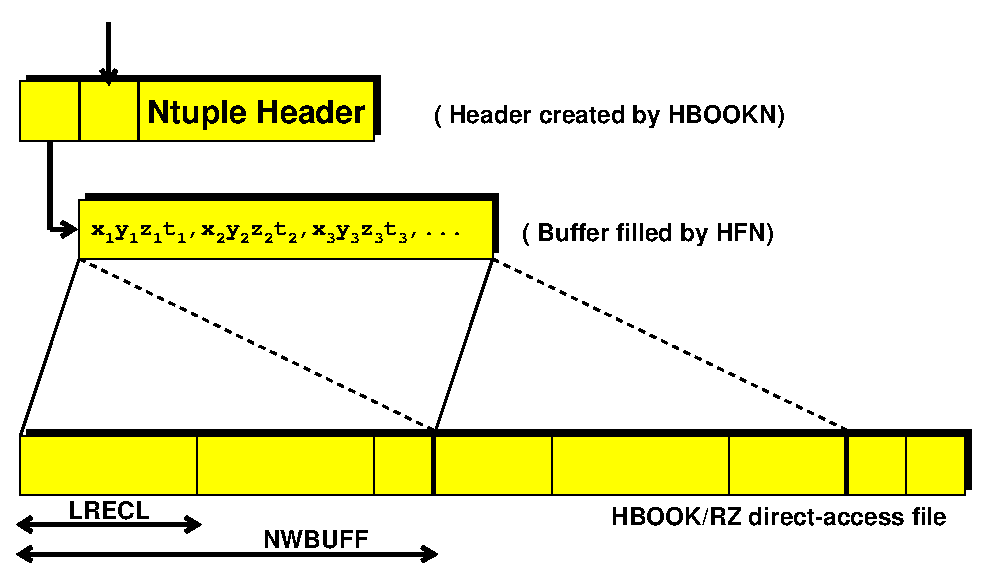
\epsfig{file=rwn.eps,width=.95\textwidth}}
\caption{Schematic structure of a RWN Ntuple}
\label{fig:rwn}
{\centering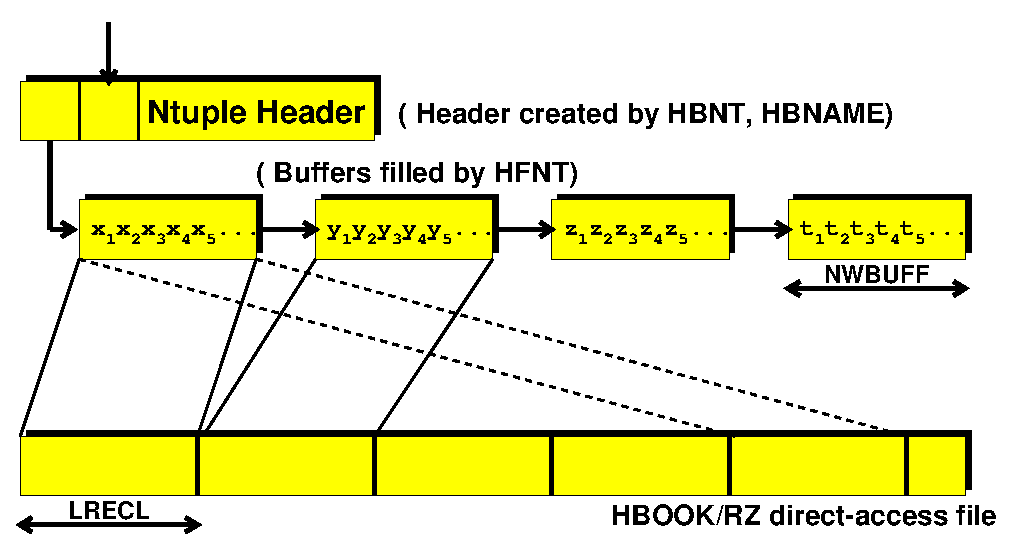
\epsfig{file=cwn.eps,width=.95\textwidth}}
\caption{Schematic structure of a CWN Ntuple}
\label{fig:cwn}
\newcommand{\III}{\(\sb{\mathtt{i}}\)}

\small

Figure~\ref{fig:cwn} shows the layout of a \CWN{} Ntuple.
The buffer size for each of the columns
\Lit{NWBUFF} was set equal to the record length \Rarg{LRECL}
(defined with routine \Rind{HROPEN}).
A \CWN{} requires a large value for the length of the common \Lit{/PAWC/},
\index{common {\tt/PAWC/}}\index{PAWC@{\tt/PAWC/} common}%
in any case larger than the number of columns
times the value \Lit{NWBUFF}, i.e. \Lit{NWPAWC>NWBUFF*NCOL}.
You can, however, expect important performance improvements by setting
the buffer size \Lit{NWBUFF} equal to a 
multiple of the record length \Rarg{LRECL} (via routine \Rind{HBSET}).

In both figures, \Lit{x\III}, \Lit{y\III}, \Lit{z\III}, 
\Lit{t\III}, etc. represent the columns of event \Lit{i}.

\end{figure}

\clearpage

\Filename{H2Row-Wise-Ntuples}
\section{Row-Wise-Ntuples (RWN)}
\label{sec:NtupleRWN}
\subsection{Booking a RWN}
\label{HNTUBOOK}
 
\Shubr{HBOOKN}{(ID,CHTITL,NVAR,CHRZPA,NWBUFF,CHTAGS)}
 
\Action Books a \RWN{} in memory or with
automatic overflow on an \Lit{RZ} file.
Only single precision floating point numbers (\Lit{REAL*4} on
32 bit machines) can be stored, no data compression is provided.

\begin{DLtt}{123456}
\item[{\rm\bf Input parameters:}]
\item[ID] Identifier of the Ntuple.
\item[CHTITL] Character
    variable containing the title associated with the Ntuple.
\item[NVAR] Number of variables per event (\Lit{NVAR\(\leq\)512})
\item[CHRZPA] Character variable containing the path
    name of a RZ file onto which the contents of the Ntuple
    can overflow.
    \begin{DLtt}{123456}
    \item[' '] {\bf Memory resident Ntuples:} \\
    \index{Ntuple!memory resident}%
        A bank of \Lit{NWBUFF} words is created.
        Further banks of the same size are added in a linear
        chain should additional space be required at filling time.
    \item['RZTOP'] {\bf Disk resident Ntuples:} (recommended) \\
    \index{Ntuple!disk resident}%
        A disk resident Ntuple is created if the \Lit{CHRZPA}
        argument specifies the top directory name of an existing RZ file
        that has already been opened with \Rind{HROPEN} or \Rind{HRFILE}.
        A bank of length \Lit{NWBUFF} is created, as in the case of 
        memory resident Ntuples. However, each time the bank becomes full
        it is automatically flushed to the RZ file, rather than
        creating additional banks in memory.
    \end{DLtt}
\item[NWBUFF]Number of words for the primary allocation for the Ntuple.
\item[CHTAGS] Character array of length \Lit{NVAR}, providing a short
    name (up to eight characters) tagging scheme for each variable.
\end{DLtt}
 
\begin{XMPt}{Example of the declaration of a memory resident RWN}
      CHARACTER*2 CHTAGS(5)
      DATA CHTAGS/'Px','Py','Pz','Q2','NU'/
 *
      CALL HBOOKN(10,'My first NTUPLE',5,' ',1000,CHTAGS)
\end{XMPt}
 
\subsection{Filling a RWN}
\label{HNTUFILL}

\Shubr{HFN}{(ID,X)}
 
\Action
Fills a \RWN{}.
 
\begin{DLtt}{123456}
\item[{\rm\bf Input parameters:}]
\item[ID] Identifier of the Ntuple.
\item[X] Array of dimension \Lit{NVAR} containing
the values for the current event.
\end{DLtt}
 
\subsection*{Memory resident Ntuples} 
\index{Ntuple!memory resident}

When a \RWN{} is booked, HBOOK reserves space in memory
in which to store the data, as specified by the \Rarg{NWBUFF}
argument of routine \Rind{HBOOKN}.
\index{memory}
As the \RWN{} is filled by a call to \Rind{HFN}, 
this space will be successively used until full. 
At that time, a new memory allocation will be made
and the process continues.

If this data is then written to disk, it appears as one
enormous logical record. 
In addition, it most cases the last block of data will 
not be completely filled thus wasting space.

If one tries to reprocess this \RWN{} at a later date,
e.g. with \PAW{}, there must be enough space in memory to
store the entire Ntuple. 
This often gives rise to problems
and so the following alternative method is recommended.

\subsection*{Circular buffer}
\index{circular buffer}

In an online environment you often want to have the last $N$ events
inside a buffer, so that the experiment can be monitored continuously.
To make it easier to handle this case, you can use routine \Rind{HFNOV},
which fills a circular buffer in memory with \RWN{} events, and when
the buffer is full, overwrites the oldest Ntuple.

\Shubr{HFNOV}{(ID,X)}
 
\Action
Fills a circular buffer with \RWN{}s.
 
\begin{DLtt}{123456}
\item[{\rm\bf Input parameters:}]
\item[ID] Identifier of the Ntuple.
\item[X] Array of dimension \Lit{NVAR} containing
the values for the current event.
\end{DLtt}

\subsection*{Disk resident Ntuples} 
\index{Ntuple!disk resident}

Prior to booking the \RWN{}, a new HBOOK RZ file is created
using \Rind{HROPEN}. 
The top directory name of this file is passed
to routine \Rind{HBOOKN} when the Ntuple is booked.

Filling proceeds as before but now, when the buffer in memory
is full, it is written to the HBOOK file and then reused
for the next elements of the Ntuple. 
This normally results in a more efficient 
utilisation of the memory,
both when the Ntuple is created and when it is reprocessed.

\begin{XMPt}{Recommended way of creating a RWN}
      PROGRAM TEST
      PARAMETER (NWPAWC = 15000)
      COMMON/PAWC/PAW(NWPAWC)
      CHARACTER*8 CHTAGS(5)
      DIMENSION EVENT(5)
      EQUIVALENCE (EVENT(1),X),(EVENT(2),Y),(EVENT(3),Z)
      EQUIVALENCE (EVENT(4),ENERGY),(EVENT(5),ELOSS)
      DATA CHTAGS/'X','Y','Z','Energy','Eloss'/
*
      CALL HLIMIT(NWPAWC)
      CALL HROPEN(1,'EXAMPLE','EXAMPLE.DAT','N',1024,ISTAT)
      IF(ISTAT.NE.0)GO TO 99
*
      CALL HBOOKN(10,'A Row-Wise-Ntuple',5,'//EXAMPLE',5000,CHTAGS)
      CALL HBOOK1(100,'Energy distribution',100,0.,100.,0.)
*
      DO 10 I=1,10000
         CALL RANNOR(X,Y)
         Z=SQRT(X*X+Y*Y)
         ENERGY=50. + 10.*X
         ELOSS=10.*ABS(Y)
         CALL HFN(10,EVENT)
         CALL HFILL(100,ENERGY,0.,1.)
 10   CONTINUE
*
      CALL HROUT(0,ICYCLE,' ')
      CALL HREND('EXAMPLE')
*
 99   CONTINUE
      END
\end{XMPt}

%\newpage%%%%%%%%%%%%%%%%%%%%%%%%%%%%%%%%%%%%%%%%%%%%%%%%%%%%%%%%%%

When the Ntuple is filled, routine \Rind{HFN} will
automatically write the buffer to the directory in the
RZ~file, which was specified in the call to \Rind{HBOOKN}
(the top directory \Lit{//EXAMPLE} in the example above).
If the current directory (CD)\index{current directory}\index{directory!current}
is different, \Rind{HFN} will save and
later automatically restore the CD.

The Ntuple created by the program shown above can be processed
by \PAW{} as follows.

\begin{XMPt}{Reading an RWN in a PAW session}
            PAW > Histo/file  1  example.dat
            PAW > Histo/plot 100
            PAW > Ntuple/plot 10.energy
            PAW > Ntuple/plot 10.eloss  energy<50
            PAW > Ntuple/plot 10.eloss%energy  x<2.and.sqrt(z)>1
\end{XMPt}

By default \Rind{HROPEN} creates a file that can be extended up to
32000 blocks, i.e. 128 Mbytes for a record length \Lit{LREC}
of 1024 words.
If one wishes to create very large Ntuples, one should
make two changes to the above procedure.

\begin{UL}
\item A large value should be used for the record length of the file,
      e.g. 8192 words (the maximum on most machines).
      {\bf N.B. the maximum record length on VMS systems is 8191 words.
      If RELATIVE access mode is used, the maximum is then 4095 words.}
      This remark does not apply to a \CWN, as described later.
\item Option \Lit{Q} on \Rind{HROPEN} should be used to override the default
      number of records allowed. 
\end{UL}

This can be achieved as by changing the previous call to \Rind{HROPEN}
as follows:

\begin{XMPt}{Writing very large Ntuple files}
              COMMON/QUEST/IQUEST(100)
              CALL HLIMIT(150000)
*
*     Create HBOOK file with the maximum record length (32756 bytes)
*     and maximum number of records (65000)
*
              IQUEST(10) = 65000
              CALL HROPEN(1,'EXAMPLE','EXAMPLE.DAT','NQ',8192,ISTAT)
              IF(ISTAT.NE.0)GO TO 99
\end{XMPt}
\index{IQUEST@{\tt IQUEST} communication vector}

\newpage%%%%%%%%%%%%%%%%%%%%%%%%%%%%%%%%%%%%%%%%%%%%%%%%%%%%%%%%%%

\Filename{H2More-general-Ntuples}
\section{More general Ntuples: Column-Wise-Ntuples (CWN)}
\label{sec:NtupleCWN}

A \CWN{} supports the storage of the following data types: floating
point numbers (\Lit{REAL*4} and \Lit{REAL*8}), integers, bit patterns
(unsigned integers), booleans and character strings.

\subsection*{Data Compression}

Floating point numbers, integers and bit patterns can be packed by
specifying a range of values or by explicitly specifying the number
of bits that should be used to store the data. Booleans are always
stored using one bit. Unused trailing array elements will not be
stored when an array depends on an index variable. In that case only
as many array elements will be stored as specified by the index
variable.

For example, the array definition \Lit{NHITS(NTRACK)} 
defines \Lit{NHITS} to depend on the index variable \Lit{NTRACK}. 
When \Lit{NTRACK} is 16, the elements \Lit{NHITS(1..16)} are stored, 
when \Lit{NTRACK} is 3, only elements \Lit{NHITS(1..3)} are stored, etc.

\subsection*{Storage Model}

Column wise storage allows direct access to any column in the Ntuple. 
Histogramming one column from a 300 column \CWN{} requires reading 
only 1/300 of the total data set. 
However, this storage scheme requires one memory buffer per column 
as opposed to only one buffer in total for an \RWN.
By default the buffer length is 1024 words, 
in which case a 100 column Ntuple requires 409600 bytes of buffer space. 
In general, performance increases with buffer size.
Therefore, one should tune the buffer size (using routine \Rind{HBSET}) 
as a function of the number of columns and the amount of available memory.
Highest efficiency is obtained when setting the buffer size equal to the
record length of the RZ HBOOK file (as specified in the call to
\Rind{HROPEN}). 
A further advantage of column wise storage is that a \CWN{}
can easily be extended with one or more new columns.

Columns are logically grouped into blocks (physically, however, all
columns are independent). 
Blocks allow users to extend a \CWN{} with private columns or to 
group relevant columns together.
New blocks can even be defined after a \CWN{} has been filled. 
The newly created blocks can be filled using routine \Rind{HFNTB}.
For example, a given experiment might define a number of standard
Ntuples. These would be booked in a section of the code that
would not normally be touched by an individual physicist. However,
with a \CWN{} a user may easily add one or more blocks of information
as required for their particular analysis.

Note that arrays are treated as a single column. 
This means that a \CWN{} will behave like a \RWN{},
with the addition of data typing and compression,
if only one array of \Lit{NVAR} elements is declared.
This is not recommended as one thereby loses
the direct column access capabilities of a \CWN{}.

\subsection*{Performance}

Accessing a relatively small number of the total number of
defined columns results in a huge increase in performance compared to
a \RWN{}.
However, reading a complete \CWN{} will take
slightly longer than reading a \RWN{} due to the overhead
introduced by the type checking and compression mechanisms and
because the data is not stored sequentially on disk.  
The performance increase with a \CWN{} will most clearly show up when 
using \PAW{}, where one typically histograms one
column with cuts on a few other columns.  
The advantages of having different data types and data compression generally
outweighs the performance penalty incurred when reading a complete \CWN{}.

\newpage%%%%%%%%%%%%%%%%%%%%%%%%%%%%%%%%%%%%%%%%%%%%%%%%%%%%%%%%%%

\subsection{Booking a CWN}
\label{HNTUBOOKT}

The booking is performed in two stages. 
Firstly, a call to \Rind{HBNT}
is made to declare the Ntuple identifier and title. 
Secondly, one or more
calls are made to \Rind{HBNAME} or \Rind{HBNAMC} to describe 
the variables that are to be stored in the Ntuple. 
Routine \Rind{HBNAMC} is used to define \Lit{CHARACTER} variables,
while all other variable types are defined with routine \Rind{HBNAME}.

\Shubr{HBNT}{(ID,CHTITL,CHOPT)}

\Action
Books a \CWN.
 
\begin{DLtt}{12345678}
\item[{\rm\bf Input parameters:}]
\item[ID]     Identifier of the Ntuple.
\item[CHTITL] Character variable specifying the title associated to the Ntuple.
\item[CHOPT]  Character variable specifying the desired options.
   \begin{DLtt}{123}
     \item[' '] for disk resident Ntuples (default).
     \item['D'] idem as \Lit{' '}.
     \item['M'] for memory resident Ntuples.
   \end{DLtt}
\end{DLtt}

The CWN{} will be stored in the current HBOOK directory.
The variables to be stored in the Ntuple will be specified
with routine \Rind{HBNAME} or \Rind{HBNAMC} described below.

When the \CWN{} will be filled with \Rind{HFNT}, the memory buffers associated 
with each column will be written to the file and directory corresponding 
to the current working directory when \Rind{HBNT} was called.
Remember that when routine \Rind{HROPEN} is called, the current
working directory is automatically set to the
top directory of that file.
It is therefore convenient to call \Rind{HBNT} immediately after \Rind{HROPEN}.
If this was not the case, routine \Rind{HCDIR} must be called prior to
\Rind{HBNT} to set the current working directory.
When the Ntuple has been filled (via calls to \Rind{HFNT})
the resident buffers in memory as well as the Ntuple header 
must be written to the file with a call to \Rind{HROUT}.
Before calling \Rind{HROUT}, the current working directory 
must be set to the current directory when \Rind{HBNT} was called.

\Shubr{HBSET}{(CHOPT,IVAL,IERR*)}

\Action
Set global Ntuple options.

\begin{DLtt}{123456}
\item[{\rm\bf Input parameters:}]
\item[CHOPT] Character variable specifying the parameter to set.
   \begin{DLtt}{1234567}
     \item['BSIZE'] Set the buffer size. For each variable (i.e.\ column)
                    a buffer of \Lit{BSIZE} words is created in memory.
                    The default for \Lit{BSIZE} is 1024.
   \end{DLtt}
\item[IVAL]   Value for the parameter specified with \Rarg{CHOPT}.
\item[{\rm\bf Output parameters:}]
\item[IERR]   Error return code (\Lit{=0} means no errors).
\end{DLtt}

If the total memory in \Lit{/PAWC/},
\index{common {\tt/PAWC/}}\index{PAWC@{\tt/PAWC/} common}%
allocated via \Rind{HLIMIT}
is not sufficient to accomodate all the column buffers of \Rarg{BSIZE} words,
then \Rind{HBNT} will automatically reduce the buffer size in such a way that all buffers can fit into
memory.
It is strongly recommended to allocate enough memory to \Lit{/PAWC/}
in such a way that each column buffer is at least equal to the block size of
the file.
A simple rule of thumb in the case of no data compression is to have 
\mbox{\Lit{NWPAWC>NCOL*LREC}}, where \Lit{NWPAWC}
is the total number of words allocated
by \Rind{HLIMIT}, \Lit{LREC} is the block size of the file in machine words
as given in the call to \Rind{HROPEN}  and \Lit{NCOL} is the number of columns.

\newpage%%%%%%%%%%%%%%%%%%%%%%%%%%%%%%%%%%%%%%%%%%%%%%%%%%%%%%%%%%

\subsection{Describing the columns of a CWN}
\label{HNTUDESC}

\Shubr{HBNAME}{(ID, CHBLOK, VARIABLE, CHFORM)}

\Shubr{HBNAMC}{(ID, CHBLOK, VARIABLE, CHFORM)}
\Action
Describe the variables to be stored in a \CWN{}
(non-character and character variables, respectively).
 
\begin{DLtt}{12345678}
\item[{\rm\bf Input parameters:}]
\item[ID]     Identifier of the Ntuple as in the call to \Rind{HBNT}.
\item[CHBLOK] Character variable of maximum length 8 characters 
              specifying the name by which the block
              of variables described by \Lit{CHFORM} is identified.
\item[VARIABLE] 
              The first variable that is described in \Lit{CHFORM}.
              Variables must be in common blocks but may not be
              in a ZEBRA bank.
              For example, given the common block \Lit{CEXAM} described
              below, one would call \Lit{HBNAME} with the argument \Lit{IEVENT}.
              In the case of character variables, the routine
              \Lit{HBNAMC} must be used. In all other cases one 
              should use \Lit{HBNAME}. 
\item[CHFORM] Can be either a character string describing the variables
              to be stored in block \Lit{CHBLOK} or:
   \begin{DLtt}{1234567}
     \item['\$CLEAR'] To clear the addresses of all variables in the Ntuple.
     \item['\$SET'] To set the addresses in which to write the values of
                    all variables in block \Lit{CHBLOK}.
   \end{DLtt}
             The last two forms are used before reading back the Ntuple data
             using \Rind{HGNT}, \Rind{HGNTB}, \Rind{HGNTV} or \Rind{HGNTF}.
             See also \Rind{HUWFUN}.
\end{DLtt}

With \Lit{CHFORM} the variables, their type, size and, possibly, range
(or packing bits) can all be specified at the same time. 
{\bf Note however that variable names should be unique, even when
they are in different blocks.}.
In the simplest
case \Lit{CHFORM} corresponds to the COMMON declaration. For example:
\begin{XMP}
       COMMON /CEXAM/ IEVENT, ISWIT(10), IFINIT(20), NEVENT, NRNDM(2)
\end{XMP}
can be described by the following \Lit{CHFORM}:
\begin{XMP}
       CHFORM = 'IEVENT, ISWIT(10), IFINIT(20), NEVENT, NRNDM(2)'
\end{XMP}
in this case the Fortran type conventions are followed and the default
sizes are taken, no packing is done. Note that to get a nice one-to-one
correspondance between the COMMON and the \Lit{CHFORM} statements
the dimension of the variables are specified in the COMMON and not
in a DIMENSION statement.

The default type and size of a variable can be overridden by
extending the variable name with \Lit{:<t>*<s>}:

\begin{tabular}{@{}>{\tt}cllcl}
\Lit{<t>} & type of variable & \Lit{<s>} values & default & routine      \\[1mm]
 R        & floating-point   & 4, 8             & 4       & \Rind{HBNAME}\\
 I        & integer          & 4, 8             & 4       & \Rind{HBNAME}\\
 U        & unsigned integer & 4, 8             & 4       & \Rind{HBNAME}\\
 L        & logical          & 4                & 4       & \Rind{HBNAME}\\
 C        & character        & \tt[4$\le$s$\le$32] (multiple of 4)
                                                & 4       & \Rind{HBNAMC}\\
\end{tabular}

\newpage%%%%%%%%%%%%%%%%%%%%%%%%%%%%%%%%%%%%%%%%%%%%%%%%%%%%%%%%%%

When the range of a type \Lit{U}, \Lit{I} or \Lit{R} variable is known, its
storage size (number of packing bits) may be added behind
the \Lit{:<t>*<s>} specification using \Lit{:<b>} for types \Lit{U}
and \Lit{I} and \Lit{:<b>:[<min>,<max>]} for type \Lit{R}. 
Floating-points are packed into an integer using:
\begin{XMP}
IPACK = ((R - <min>)/(<max> - <min>)*(2**<b> - 1) + 0.5
\end{XMP}

When \Lit{:<b>...} is not specified a variable is stored using the
number of bytes given by \Lit{<s>} or the default. 
In case the default type and size of a variable should be used, the
packing bits can be specified as \Lit{::<b>...}. 
\Lit{<b>} must be in the range \Lit{1}\(\le\)\Lit{b}\(\le\)\Lit{8*<s>}.
Automatic bit packing will happen, for type \Lit{U} and \Lit{I}, when a range
is specified like: \Lit{ICNT[-100,100]}. In this case \Lit{ICNT} will
be packed in 8 bits (7 bits for the integer part and 1 bit for the sign).
In case \Lit{CNT} is an integer ranging from -100 to 100 it could be
specified either like \Lit{CNT[-100,100]:I} or like \Lit{CNT:I::[-100,100]}.
Logical variables will always be stored in 1 bit.
All variables must be aligned on a word boundary and character variables
must have a length modulo 4. The maximum length of the variable name
is 32 characters.

Variable-length Ntuple rows and looping over array components
are also supported to optimize Ntuple storage and Ntuple plotting.
Variable row length can occur when arrays in the Ntuple
depend on an index variable.

\begin{XMPt}{Example of a variable row length CWN definition}
      PARAMETER (MAXTRK = 100, MAXHIT = 300)
      COMMON /CMTRK/ NTRACK, NHITS(MAXTRK), PX(MAXTRK), PY(MAXTRK),
     +               PZ(MAXTRK), XHITS(MAXHIT,MAXTRK), YHITS(MAXHIT,MAXTRK),
     +               ZHITS(MAXHIT,MAXTRK)
      CALL HBNAME(ID,'VARBLOK2',NTRACK, 
     +            'NTRACK[0,100], NHITS(NTRACK)[0,300],'//
     +            'PX(NTRACK), PY(NTRACK), PZ(NTRACK), XHITS(300,NTRACK),'//
     +            'YHITS(300,NTRACK), ZHITS(300,NTRACK)')
\end{XMPt}

In this example the number of elements to store in one Ntuple row
depends on the number of tracks, \Lit{NTRACK}.
The call to \Rind{HBNAME} declares \Lit{NTRACK} to be an
index variable and that the size of the Ntuple row depends on the value of 
this index variable.
The range of an index variable is specified using \Lit{[<l>,<u>]},
where \Lit{<l>} is the lower and \Lit{<u>} the upper limit of the arrays
using this index variable. In the above example the 
lower limit of \Lit{NTRACK} is 0 and the upper limit is 100 (\Lit{= MAXTRK}).
While filling a \CWN{} HBOOK can also easily test for
array out-of-bound errors since it knows the range of \Lit{NTRACK}.
Only the last dimension of a multi-dimensional array may be variable
and the index variable must be specified in the block where it is used.
Array lower bounds must, just like the lower range of the index variable,
be 0.

\Rind{HBNAME} may be called more than once per block as long as no data
has been stored in the block. 
New blocks can be added to an Ntuple at any time, even after filling has started,
whereas existing blocks may only be extended before filling has started.
\index{block}


\subsection*{Alternative way of booking a CWN}

\Shubr{HBOOKNC}{(ID,CHTITL,NVAR,BLOCK,TUPLE,CHTAGS)}

\Action Provides a way to define a \CWN{} similar to 
\Rind{HBOOKN} for a \RWN{}.

\begin{DLtt}{123456}
\item[{\rm\bf Input parameters:}]
\item[ID] Identifier of the CWN{}.
          If it does not already exist, it is created.
\item[CHTITL] Character variable specifying the name of the Ntuple
          (not used if it already exists).
\item[NVAR]  Number of variables per event (maximum 200).
\item[BLOCK] Name of the block inside the \CWN (default is \Lit{'Block1'}.
\item[TUPLE] Array of dimension \Lit{NVAR} that will contain values at filling
                 time.
\item[CHTAGS] Character array of length \Lit{NVAR}, providing a short
    name (up to eight characters) tagging scheme for each variable.
\end{DLtt}

\subsection{Filling a CWN}
\label{HNTUFILLT} 

\Shubr{HFNT}{(ID)}
 
\Action Fill a \CWN{}.
 
\begin{DLtt}{123456}
\item[{\rm\bf Input parameter:}]
\item[ID] Identifier of the CWN{}.
\end{DLtt}
\Rind[HROPEN]{}
\Rind[HBNT]{}
\Rind[HBNAME]{}
\Rind[HBNAMC]{}
\Rind[HFNT]{}
\Rind[HROUT]{}
\Rind[HREND]{}
\index{PAW}


\Shubr{HFNTB}{(ID,CHBLOK)}
 
\Action Fill the named block \Lit{CHBLOK} in a \CWN{}.
 
\begin{DLtt}{123456}
\item[{\rm\bf Input parameters:}]
\item[ID] Identifier of the Ntuple.
\item[CHBLOK]Character variable specifying the block that is to be filled.
\end{DLtt}

\Shubr{HPRNT}{(ID)}
 
\Action Print the  definition of the CWN{} \Lit{ID} as 
defined by the calls to \Rind{HBNAME} and/or \Rind{HBNAMC}.
 
\begin{DLtt}{123456}
\item[{\rm\bf Input parameter:}]
\item[ID] Identifier of the CWN{}.
\end{DLtt}

\subsection*{Recovery procedure}
\label{sec:Ntuple-recovery}

The Ntuple header, containing the essential
definitions associated with an Ntuple,
are now written to the output file when the first
buffer is written. 
If the job producing the Ntuple does not terminate in a clean way 
(i.e. the job crashs or you forgot to call \Rind{HROUT}), 
it is now possible to rebuild the Ntuple header from the 
information available in the file.
Note, however, that the events corresponding to the last 
Ntuple buffer in memory are lost.

\Shubr{HRECOV}{(ID,CHOPT)}

\Action Recover the information associated with a \CWN{}.
 
\begin{DLtt}{123456}
\item[{\rm\bf Input parameters:}]
\item[ID]    Identifier of the CWN{}.
\item[CHOPT] Character variable specifying the option desired.
             At present Not used at present; \Lit{' '}
             should be specified
\end{DLtt}

\newpage%%%%%%%%%%%%%%%%%%%%%%%%%%%%%%%%%%%%%%%%%%%%%%%%%%%%%more com

\begin{XMPt}{Example of saving contents of common variables in an Ntuple}
        COMMON/GCFLAG/IDEBUG,IDEMIN,IDEMAX,ITEST,IDRUN,IDEVT,IEORUN
       +        ,IEOTRI,IEVENT,ISWIT(10),IFINIT(20),NEVENT,NRNDM(2)

        COMMON/GCTRAK/VECT(7),GETOT,GEKIN,VOUT(7),NMEC,LMEC(MAXMEC)
       + ,NAMEC(MAXMEC),NSTEP ,MAXNST,DESTEP,DESTEL,SAFETY,SLENG
       + ,STEP  ,SNEXT ,SFIELD,TOFG  ,GEKRAT,UPWGHT,IGNEXT,INWVOL
       + ,ISTOP ,IGAUTO,IEKBIN, ILOSL, IMULL,INGOTO,NLDOWN,NLEVIN
       + ,NLVSAV,ISTORY

        COMMON/GCTMED/NUMED,NATMED(5),ISVOL,IFIELD,FIELDM,TMAXFD,DMAXMS
       +      ,DEEMAX,EPSIL,STMIN,CFIELD,PREC,IUPD,ISTPAR,NUMOLD

        CHARACTER*4 TYPE
        COMMON/CMCC/TYPE

*     The code to book and fill the Ntuple would look like this:
*
*   Initialisation phase.
*   The calls to HROPEN, HBNT and HBNAME may be placed in different 
*   initialisation routines. 
*   In this example example the Ntuple will be stored in directory //MYFILE.
*
        CALL HROPEN(1,'MYFILE','geant.ntup','N',1024,ISTAT)
        CALL HBNT(10,'Geant Ntuple',' ')
*
        CALL HBNAME(10, 'RUN',    IDRUN,  'IDRUN::16,IDEVT::16')
        CALL HBNAME(10, 'RUN',    IEORUN, 'IEORUN::16')
        CALL HBNAME(10, 'VECT',   VECT,   'VECT(6)')
        CALL HBNAME(10, 'GEKIN',  GEKIN,  'GEKIN')
        CALL HBNAME(10, 'INWVOL', INWVOL, 'INWVOL[1,7],ISTOP[1,7]')
        CALL HBNAME(10, 'NUMED',  NUMED,  'NUMED::10')
        CALL HBNAME(10, 'NSTEP',  NSTEP,  'NSTEP::16')
        CALL HBNAMC(10, 'TYPE',   TYPE,   'TYPE:C')
*
*    To fill the Ntuple, when the common blocks are filled just invoke
*    routine HFNT which knows the addresses and the number of variables.
*
        DO 10 I = 1, 1000000
           ...
           CALL HFNT(10)
10      CONTINUE
*
*                      At the end of the job, proceed as usual
*
        CALL HROUT(10, ICYCLE, ' ')
        CALL HREND('MYFILE')

\end{XMPt}

\newpage%%%%%%%%%%%%%%%%%%%%%%%%%%%%%%%%%%%%%%%%%%%%%%

\begin{changebar}
\subsection*{Disk resident Ntuples}

Histograms are never created directly on a disk file. 
They are always created in the current directory in memory 
(\Lit{//PAWC} or \Lit{//PAWC/subdir}).
Histograms are saved on the disk file with a call of type 
\Lit{CALL \Rind{HROUT}}
In case of disk-resident Ntuples, it is the same thing. 
The Ntuple header 
(data structure containing the column names) is always created
in the current directory in memory 
(\Lit{//PAWC} or \Lit{//PAWC/subdir}).
However, the call to \Rind{HBNT} remembers the current 
directory on disk (in the case below
the \Lit{CD} on disk is \Lit{//K0}). 
When you fill the Ntuple, \Rind{HFNT} fills a buffer in memory. 
When this buffer is full, \Rind{HFNT} knows what is the \Lit{CD} on disk.
The buffer is written into that directory. 
Note that your current directory on disk may be somewhere else. 
\Rind{HFNT} will temporarely change the \Lit{CD} to \Lit{//K0} 
and will reset the \Lit{CD} to what it was before calling \Rind{HFNT}.
At the end of your job, you have to save the header and the current buffer
in memory on the disk file. 
For that you have to:

\begin{UL}
\item[--] Change the directory in memory where you book the ntuple. 
          If you do not have subdirectories, 
          this operation is not necessary.
\item[--] Change the directory on disk where you specified it in 
          \Rind{HBNT}. 
          In the case below \Lit{//KO}.
\item[--] Issue a call to \Rind{HROUT} or \Rind{HREND}.
\end{UL}

\begin{XMPt}{Creating a disk resident Ntuple}
      call HCDIR('//PAWC',' ')
*--     HROPEN sets the directory to //K0, so no call to HCDIR is needed
      call HROPEN(50,'K0','~/mydir/K0.rz','N',1024,ISTAT)
      if (ISTAT.ne.0) write(6,*) 'Error in HROPEN'
      call HBNT(1000,'NTuple','D')
      call HLDIR('//PAWC','T') ! Now you can see the header in //PAWC
      call HLDIR('//K0','T')   ! OK, nothing yet on //K0
*--     HBNAME describes the Ntuple
      call HBNAME(1000,'Event',EvtNo,
     +            'RunNo:I,Evtno:I,NPos:I,NNeg:I,'//
     +            ....
....
        call HLDIR('//K0','T') ! Nothing yet on //K0
        call HCDIR('//K0',' ') ! Useless, HFNT remembers that buffers are written to //KO
        call HFNT(1000)
        call HLDIR(' ','T')    ! This will not show anything on //K0.
                               ! However if you call HLDIR(' ','TA') you will see all Ntuple 
                               ! extensions in the case you have many calls to HFNT. 
                               ! In this particular example everything is still in memory.
....
      call HCDIR('//K0',' ')   ! Useless, you are already here
      call HLDIR('//K0',' ')   ! same as call hldir(' ','T')
      call RZLDIR(' ',' ')
      call HROUT(0,icycle,' ')
*-*      If you call HLDIR(' ',' ') here you will see the header
*-*      If you call HLDIR(' ','A') here you will see the header and your Ntuple extensions
      call HREND('K0')
\end{XMPt}
\end{changebar}

\newpage%%%%%%%%%%%%%%%%%%%%%%%%%%%%%%%%%%%%%%%%%%%%%%

\Filename{H2Making-projection-of-a-RWN}
\section{Making projections of a RWN}
\label{HNTUPROJ} 

\Shubr{HPROJ1}{(ID,IDN,ISEL,FUN,IFROM,ITO,IVARX)}
 
\Action
Fill an existing one-dimensional histogram with data from a RWN.
 
\begin{DLtt}{123456}
\item[{\rm\bf Input parameters:}]
\item[ID]    Identifier of a 1-dimensional histogram, which
             must have been previously booked with \Rind{HBOOK1}.
\item[IDN]   Identifier of the RWN Ntuple.
\item[ISEL]  Selection flag
             \begin{DLtt}{1234}
                \item[0]   No selection criterion. All events between \Lit{IFROM} and
                           \Lit{ITO} are histogrammed with a weight of one.
                \item[<>0] The function \Lit{FUN} is called for each event
                           between \Lit{IFROM} and \Lit{ITP}, which are histogrammed
                           with as weight the value of \Lit{FUN}. of one.
             \end{DLtt}
\item[FUN]   User function, to be declared \Lit{EXTERNAL} in the calling
             routine. It has as parameters the array of variables \Lit{X} and the
             selection flag \Lit{ISEL}. If \Lit{FUN=0.},
             no filling takes place for that event.
\item[IFROM] Event number where the histogramming has to start.
\item[ITO]   Event number where the histogramming has to end.
\item[IVARX] Sequence number in the Ntuple of the variable to be
             histogrammed
\end{DLtt}

\begin{XMPt}{Example of the use of a one-dimensional Ntuple projection}
     PROGRAM MAIN
     EXTERNAL WFUNC
     CALL HPROJ1(10,20,1,WFUNC,0,0,4)
     .....

     FUNCTION WFUNC(X,ISEL)
     DIMENSION X(*)
     WFUNC=0.
     IF(ISEL.EQ.1)THEN
         IF(X(2)**2 +X(3)**2.LT.0.)WFUNC=1.
     ELSEIF(ISEL.EQ.2)THEN
         IF(X(2)**2 +X(3)**2.GT.5.)WFUNC=1.
     ELSE
         WFUNC=X(5)
     ENDIF
     END
\end{XMPt}

Note that in an interactive session with \PAW{},
the user function \Lit{FUN} can be defined
interactively using a Fortran-like syntax without recompilation
and relinking.
 
\Shubr{HPROJ2}{(ID,IDN,ISEL,FUN,IFROM,ITO,IVARX,IVARY)}
 
\Action
Same action as \Rind{HPROJ1}, but filling a previously
booked 2-dimensional histogram or a profile histogram.
Variable \Lit{X(IVARX)} will be projected onto the \Lit{X} axis and
\Lit{X(IVARY)} onto the \Lit{Y} axis for all entries in the Ntuple
between \Lit{IFROM} and \Lit{ITO} inclusive.
 
The number of entries in an Ntuple can be obtained by \Rind{HNOENT}.
 
\newpage%%%%%%%%%%%%%%%%%%%%%%%%%%%%%%%%%%%%%%%%%%%%%%%%%%%%%%%%%%%%%%%

\Filename{H2Get-information-about-an-Ntuple}
\section{Get information about an Ntuple}
 
\Shubr{HGIVEN}{(ID,CHTITL*,*NVAR*,CHTAG*,RLOW*,RHIGH*)}
 
\Action
Routine to provide information about an Ntuple.
 
\begin{DLtt}{123456}
\item[{\rm\bf Input parameters:}]
\item[ID] Identifier of the Ntuple.
\item[NVAR] Dimension of arrays \Lit{TAGS}, \Lit{RLOW}
and \Lit{RHIGH}.
\item[{\rm\bf Output parameters:}]
\item[CHTITL] Character
variable containing the title associated with the Ntuple.
\item[NVAR] The original contents is overwritten by the actual dimension of the Ntuple.
If \Lit{ID1} does not exist or is not an Ntuple \Lit{NVAR=0} is returned.
\item[CHTAG] Character array of dimension \Lit{NVAR}, which
contains the tag names of the Ntuple elements.
\item[RLOW] Array of dimension \Lit{NVAR}, which
contains the lowest value for each Ntuple element.
\item[RHIGH] Array of dimension \Lit{NVAR}, which
contains the highest value for each Ntuple element.
\end{DLtt}
 
\subsection{Retrieve the contents of a RWN into an array}
 
\Shubr{HGN}{(ID,*IDN*,IDNEVT,X*,IERROR*)}
 
\Action
Copy the contents of a \RWN{} event into an array.
 
\begin{DLtt}{123456}
\item[{\rm\bf Input parameters:}]
\item[ID]     Identifier of the Ntuple.
\item[IDN]    Must be initialized to zero before the first call to \Rind{HGN}.
\item[IDNEVT] Event number
\item[{\rm\bf Output parameters:}]
\item[IDN]    Internal HBOOK pointer
\item[X]      Array to contain variables for the event chosen.
\item[IERROR] Error return code.
\end{DLtt}

This routine returns in the vector \Lit{X} the contents of the 
row \Lit{IDNEVT} or Ntuple \Lit{ID}. 
The vector \Lit{X} must be of size \Lit{NVAR},
as specified in the call to \Rind{HBOOKN}.
If more than one row of the Ntuple is to be processed, it is more
efficient to call first \Rind{HGNPAR} and then \Rind{HGNF}.

\Shubr{HGNPAR}{(ID,CHROUT)}

\Action
Obtains the address and parameters of Ntuple ID.
\begin{DLtt}{123456}
\item[{\rm\bf Input parameters:}]
\item[ID]Identifier of the Ntuple.
\item[CHROUT]Character variable containing the name of the calling
subroutine (printed in case of errors).
\end{DLtt}

This routine sets some internal pointers and must be called before
the first call to \Rind{HGNF} for a given \RWN{}. When accessing
more than one row of an Ntuple it is more efficient to call
\Rind{HGNPAR} and then \Rind{HGNF} for each row that is required
than to call \Rind{HGN}.

\Shubr{HGNF}{(ID,IDNEVT,X*,IERROR*)}
 
\Action
Copy the contents of an Ntuple event into an array.
The routine \Rind{HGNPAR} must have been called
prior to the first call to \Rind{HGNF} for a given
Ntuple.
 
\begin{DLtt}{123456}
\item[{\rm\bf Input parameters:}]
\item[ID]Identifier of the Ntuple.
\item[IDNEVT]Event number
\item[{\rm\bf Output parameters:}]
\item[X] Array to contain variables for the event chosen.
\item[IERROR] Error return code.
\end{DLtt}

This routine returns in the vector \Lit{X} the contents of the 
row \Lit{IDNEVT} or Ntuple \Lit{ID}. 
The vector \Lit{X} must have be of size \Lit{NVAR},
as specified in the call to \Rind{HBOOKN}.

\begin{XMPt}{Example of access to RWN information}
\NODOC{\baselineskip=.95\baselineskip\relax}      PROGRAM TEST
      INTEGER    NWPAWC
      PARAMETER (NWPAWC=15000, MTUPLE=5)
      COMMON/PAWC/PAW(NWPAWC)
      CHARACTER*80 CHTITL
      CHARACTER*8 CHTAGS(MTUPLE),CHTAGZ(MTUPLE)
      DIMENSION EVENT(MTUPLE),RLOW(MTUPLE),RHIGH(MTUPLE)
      EQUIVALENCE (EVENT(1),X),(EVENT(2),Y),(EVENT(3),Z)
      EQUIVALENCE (EVENT(4),ENERGY),(EVENT(5),ELOSS)
      DATA CHTAGS/'X','Y','Z','Energy','Eloss'/
*-- Tell HBOOK how many words are in PAWC.
      CALL HLIMIT(NWPAWC)
*-- Book Ntuple 
      CALL HBOOKN(10,'A Row-Wise-Ntuple',5,' ',5000,CHTAGS)
*-- Fill the Ntuple 
      DO 10 I=1,1000
         CALL RANNOR(X,Y)
         Z=SQRT(X*X+Y*Y)
         ENERGY=50. + 10.*X
         ELOSS=10.*ABS(Y)
         CALL HFN(10,EVENT)
 10   CONTINUE
*--   Obtain the definitions of the Ntuple
      NVAR = MTUPLE
      CALL HGIVEN(10,CHTITL,NVAR,CHTAGZ,RLOW,RHIGH)
      PRINT *,'Definitions of Ntuple # ',10
      PRINT *,'   Title: ',CHTITL(1:LENOCC(CHTITL))
      PRINT *,'   Number of variables: ',NVAR
      DO 20 I=1,NVAR
         PRINT 9001,I,RLOW(I),RHIGH(I)
9001  FORMAT(' Min/Max values for column # ',I3,1X,F10.5,
     +       1X,F10.5)
 20   CONTINUE
*--   Get the contents of 'event' # 333
      CALL HGNPAR(10,'TEST')
      CALL HGNF(10,333,EVENT,IERR)
      PRINT *,IERR,EVENT
*--   Get the number of events in this Ntuple
      CALL HNOENT(10,NEVENT)
      PRINT *,NEVENT
 99   CONTINUE
      END
\end{XMPt}

\newpage%%%%%%%%%%%%%%%%%%%%%%%%%%%%%%%%%%%%%%%%%%%%%%%%%%%%%%%%%%

\subsection{Retrieve the contents of a CWN into a common block}
 
\Shubr{HGNT}{(ID,IDNEVT,IERR*)}
 
\Action

Retrieve information about a \CWN{} row.
 
\begin{DLtt}{123456}
\item[{\rm\bf Input parameters:}]
\item[ID] Identifier of the Ntuple.
\item[IDNEVT] Number of the event about which information is required.
\item[{\rm\bf Output parameter:}]
\item[IERR] Error return code (\Lit{=0} if event was found)
\end{DLtt}

The information is restored at the addresses specified by \Rind{HBNAME}
or \Rind{HBNAMC} (for \Lit{CHARACTER} data).
If the information is being retrieved by a program other than the
one that wrote the Ntuple then \Rind{HBNAME}
or \Rind{HBNAMC} must be called as appropriate (see below).
\begin{XMP}
      CALL HBNAME(ID,' ',0,'$CLEAR')
      CALL HBNAME(ID,CHBLOK,VARIABLE,'$SET')
\end{XMP}
\Rind[HBNAME]{}
\Rind[HBNAMC]{}
These calls are required as \Lit{HBOOK} must obtain the location
at which the requested information is to be returned which is
obviously not valid between programs.
The first call clears all the addresses stored by \Lit{HBOOK}
for the specified Ntuple and the second one sets the
addresses for the variables in block \Lit{CHBLOK} starting at variable
\Lit{VARIABLE}. The second call should be repeated for every block of
which data has to be retrieved. The routine \Rind{HUWFUN} will generate
these calls automatically in the skeleton user function.

\Shubr{HGNTB}{(ID,CHBLOK,IROW,IERR*)}
 
\Action

Retrieve information about a named block in an Ntuple row.
 
\begin{DLtt}{123456}
\item[{\rm\bf Input parameters:}]
\item[ID] Identifier of the Ntuple.
\item[CHBLOK]Character variable specifying the block that is to be
retrieved.
\item[IROW] Number of the row about which information is required.
\item[{\rm\bf Output parameter:}]
\item[IERR] Error return code (\Lit{=0} if row was found)
\end{DLtt}

The information is restored at the addresses specified by \Rind{HBNAME}
or \Rind{HBNAMC} (for \Lit{CHARACTER} data).

\Shubr{HGNTV}{(ID,CHVAR,NVAR,IROW,IERR*)}
 
\Action

Retrieve information about the named variables in an Ntuple row.
 
\begin{DLtt}{123456}
\item[{\rm\bf Input parameters:}]
\item[ID] Identifier of the Ntuple.
\item[CHVAR] Array of character variables specifying the variables
             that are to be retrieved.
\item[NVAR]  Number of character variables specified in \Lit{CHVAR}.
\item[IROW] Number of the row about which information is required.
\newpage%%%%%%%%%%%%%%%%%%%%%%%%%%%%%%%%%%%%%%%%%%%%%%%%%%%%%%%%%%%%%%%%
\item[{\rm\bf Output parameter:}]
\item[IERR] Error return code (\Lit{=0} if row was found)
\end{DLtt}

The information is restored at the addresses specified by \Rind{HBNAME}
or \Rind{HBNAMC} (for \Lit{CHARACTER} data).

\begin{changebar}
You should only call \Rind{HBNAME} for the blocks that 
contain variables you want to read using \Rind{HGNTV}. 
If you call \Rind{HBNAME} for all blocks you should
have a \Lit{PAWC} which is at least the same size as the one you used to
create the Ntuple. 
If not you will run out of memory.

Also changing the buffer size will not help because the buffer used for
reading will be the same size as the buffer used to write the Ntuple.

There is a special option in \Rind{HBNAME} with which you can tell
\Rind{HBNAME} to only set the address 
for a single variable in a block (this option
is used by PAW to reduce memory usage). 

To set the address for a single variable call 
\Rind{HBNAME} (or \Rind{HBNAMC}) as follows:
\begin{XMP}
      CALL HBNAME(ID, BLOCK, IADDR, '$SET:NTVAR')
\end{XMP}
This will tell \Rind{HGNTV} to restore the Ntuple 
variable \Lit{NTVAR} in address \Lit{IADDR}. 
Using this form of \Rind{HBNAME} will only reserve buffer space for
the variables you plan to read and not for all variables in the block.
However, you have to be careful that when you change the list 
of variable for
\Rind{HGNTV} to also add or remove the correct \Rind{HBNAME} calls.
\end{changebar}

\Shubr{HGNTF}{(ID,IROW,IERR*)}
 
\Action

Retrieve information about all variables specified in a previous
call to either \Rind{HGNT}, \Rind{HGNTB} or \Rind{HGNTV}, in an Ntuple row.
This routine is much faster than either \Rind{HGNT}, \Rind{HGNTB} or
\Rind{HGNTV}.
 
\begin{DLtt}{123456}
\item[{\rm\bf Input parameters:}]
\item[ID] Identifier of the Ntuple.
\item[IROW] Number of the row about which information is required.
\item[{\rm\bf Output parameter:}]
\item[IERR] Error return code (\Lit{=0} if row was found)
\end{DLtt}

The information is restored at the addresses specified by \Rind{HBNAME}
or \Rind{HBNAMC} (for \Lit{CHARACTER} data).

\newpage%%%%%%%%%%%%%%%%%%%%%%%%%%%%%%%%%%%%%%%%%%%%%%%%%%%%%%%%%%%%%

\subsection{Generate a user function}
\label{sec:userfunction}

HBOOK can automatically produce a skeleton user selection
function, which includes the Ntuple declaration via
the calls \Rind{HBNT}, \Rind{HBNAME} and \Rind{HBNAMC},
and can be used in a later run to access the elements of 
the Ntuple.
Two cases are available; one for use in batch and the other for use with
\PAW.
In the first case the common block names will be those
specifed by the user in the call to \Rind{HBNAME} or \Rind{HBNAMC}. 
For \PAW{}, these common names are
\Lit{/PAWCR4/}, \Lit{/PAWCR8/} and \Lit{/PAWCCH/} for storing
the ``single precision'' (\Lit{LOGICAL}, \Lit{INTEGER} and \Lit{REAL*4}),
``double precision'' (\Lit{REAL*8} and \Lit{COMPLEX}) and
\Lit{CHARACTER} data respectively.

\Shubr{HUWFUN}{(LUN,ID,CHFUN,ITRUNC,CHOPT)}
 
\Action

Write an user function or subroutine to access an Ntuple.
 
\begin{DLtt}{123456}
\item[{\rm\bf Input parameters:}]
\item[LUN] Logical unit used to write the user routine.
           \Lit{LUN} must be opened before this call.
\item[ID] Identifier of the Ntuple.
\item[CHFUN] Character variable specifying the routine name.
\item[ITRUNC] All variable names will be truncated to \Lit{ITRUNC}
              characters. \Lit{ITRUNC=0} is no truncation.
\item[CHOPT]  Character variable specifying the desired options.
   \begin{DLtt}{1234}
     \item['B'] Make an user subroutine for batch usage (i.e.
                with \Rind{HBNAME} and \Rind{HBNAMC} calls) (default).
     \item['P'] Make a \PAW{} selection function.
   \end{DLtt}
\end{DLtt}

A simple example of the two kinds of skeletons generated with
routine \Rind{HUWFUN} is given below. 
Another more complex example can be found on page \pageref{sec:staffskeleton},
where the code of a fully worked out subroutine based on such
a sketeton can also be studied.

In \PAW{}, the command \Lit{UWFUNC} generates a skeleton for the
\RWN{} or \CWN{} analysis function automatically.

\newpage %%%%%%%%%%%%%%%%%%%%%%%%%%%%%%%%%%%%%%%%%%%%%%%%%%%%%%%%%%%%

\begin{XMPt}{Example of an Ntuple definition and HUWFUN usage}
      COMMON /CVECT/ V1, V2, V3, V4, V5, V6, V7, V8, V9, V10,
     +               V11, V12, V13, V14, V15, V16, V17, V18, V19, V20
      ...
      ...
*
*-- book N-tuple 20
*
      CALL HBNT(20,'1 block 20 variable N-tuple', ' ')
      CALL HBNAME(20,'VECT',V1,'V1,V2,V3,V4,V5,V6,V7,V8,V9,V10,V11,
     +                          V12,V13,V14,V15,V16,V17,V18,V19,V20')
*
      ...
      OPEN(11,FILE='nt20.f',STATUS='UNKNOWN')
      OPEN(12,FILE='nt20p.f',STATUS='UNKNOWN')
      CALL HUWFUN(11, 20, 'NT20', 0, 'B')
      CALL HUWFUN(12, 20, 'NT20', 0, 'P')
      ...
\end{XMPt}
The \Rind{HUWFUN} output files \Lit{nt20.f} and \Lit{nt20p.f} look like:
\begin{XMPt}{File nt20.f}
      SUBROUTINE NT20
*********************************************************
*                                                       *
* This file was generated by HUWFUN.                    *
*                                                       *
*********************************************************
*
*     N-tuple Id:     20
*     N-tuple Title:  1 block 20 variable N-tuple
*     Creation:       11/06/92 18.46.10
*
*********************************************************
*
      REAL V1,V2,V3,V4,V5,V6,V7,V8,V9,V10,V11,V12,V13,V14,V15,V16,V17
     + ,V18,V19,V20
      COMMON /VECT/ V1,V2,V3,V4,V5,V6,V7,V8,V9,V10,V11,V12,V13,V14,V15
     + ,V16,V17,V18,V19,V20
*
      CALL HBNAME(20,' ',0,'$CLEAR')
      CALL HBNAME(20,'VECT',V1,'$SET')
*

*
*--   Enter user code here
*

*
      END
\end{XMPt}

\newpage%%%%%%%%%%%%%%%%%%%%%%%%%%%%%%%%%%%%%%%%%%%%%%%%%%%%%%%%%%%%%%

\begin{XMPt}{File nt20p.f}
      REAL FUNCTION NT20()
*********************************************************
*                                                       *
* This file was generated by HUWFUN.                    *
*                                                       *
*********************************************************
*
*     N-tuple Id:     20
*     N-tuple Title:  1 block 20 variable N-tuple
*     Creation:       11/06/92 18.46.10
*
*********************************************************
*
      COMMON /PAWIDN/ IDNEVT,VIDN1,VIDN2,VIDN3,VIDN(10)
*
      REAL V1,V2,V3,V4,V5,V6,V7,V8,V9,V10,V11,V12,V13,V14,V15,V16,V17
     + ,V18,V19,V20
      COMMON /PAWCR4/ V1,V2,V3,V4,V5,V6,V7,V8,V9,V10,V11,V12,V13,V14
     + ,V15,V16,V17,V18,V19,V20
*

*
*--   Enter user code here
*

      NT20 = 1.
*
      END
\end{XMPt}

\subsection{Optimizing event loops}

\PAW{} is able, before starting the loop over the events, to find out
which are the columns of the \CWN{} which are actually referenced
in any given query (command line selection expression or COMIS routine).
Only the columns which are referenced will be read from the file.

If you  analyse Ntuple data without \PAW{}, it is your own
responsibility to find out and specify which are the columns
referenced via the routines \Rind{HGNTV} or \Rind{HGNTB} (if all variables
in a block are needed).

This optimization can be very important.
Assume, for instance, that a
100 Mbyte file contains an Ntuple consisting of
300 columns, and that 3 columns are referenced.
Then without optimization
the complete 100 Mbyte file will have to be read, while, by specifying
the columns used, only 1 Mbyte will be input.

%\newpage%%%%%%%%%%%%%%%%%%%%%%%%%%%%%%%%%%%%%%%%%%%%%%%%%%%%%%%%%%
%
%\section{Using Ntuples with PAW}
%\index{PAW}
%
%In PAW, the \Ucom{NTUPLE/SCAN} command displays correctly each column
%taking into account the data types.
%
%In the selection formula of commands like \Ucom{NTUPLE/PLOT} it
%is possible to compare character variables and constants. 
%Boolean operations on bit-pattern data types are also supported.
%
%It is also possible to histogram
%all the components of an array in one single command, e.g.
%\begin{XMP}
%    PAW > \Ucom{Ntuple/plot 10.vect(1)}   generates 1 histogram (1000000),
%    PAW > \Ucom{Ntuple/plot 10.vect(4:6)} generates 3 histograms,
%    PAW > \Ucom{Ntuple/plot 10.vect(1:6)} generates 6 histograms, etc.
%\end{XMP}
%To get a histogram of the sum of the components of the array, we type:
%\begin{XMP}
%    PAW > \Ucom{Ntuple/plot 10.vect}      generates 1 histogram with the sum of
%                                   the 6 array components.
%\end{XMP}
%
%There are two ways of using CWN{} variables in PAW:
%
%\begin{itemize}
%\item If an explicit dimension has been specified for a variable with \Rind{HBNAME}, e.g.\\
%      \Lit{CALL HBNAME(10,'VBLOK',VAR,'VAR(50)'}\\
%      then a command like \Ucom{NTUPLE/PLOT 10.VAR} will generate 50 histograms,
%      one for each of the declared variable elements of \Lit{VAR}.
%\item If an implicit dimension is given for a variable, e.g. \\
%      \Lit{CALL HBNAME(10,'TBLOK',NTRACK,'NTRACK,PX(NTRACK),PY(NTRACK),PZ(NTRACK)'}\\
%      then PAW assumes that one wants to plot all instances of the given variables 
%      (\Lit{PX}, \Lit{PY} or \Lit{PZ}) in the same histogram, summing over all entries \Lit{NTRACK}. 
%      Thus the command \Ucom{NTUPLE/PL 10.PX} would add \Lit{NTRACK} entries into one 
%      histogram. Of course \Ucom{NTUPLE/PL 10.PX(1)} would only enter the value for the
%      first instance of variable \Lit{PX} into the histogram for each event.
%\end{itemize}
%
%For both type of Ntuples (\RWN{} and |CWN) the command \Ucom{UWFUNC} 
%generates the selection function with the
%correct declaration of the data types (see the discussion of 
%the generation of the user function \Rind{HUWFUN}
%on page \pageref{sec:userfunction}).
%
%
%\newpage%%%%%%%%%%%%%%%%%%%%%%%%%%%%%%%%%%%%%%%%%%%%%%%%%%%%%%%%%
%
%\Section{4cm}{Ntuple chains with PAW}
%
%With the current implementation of PAW, in order to process
%many files containing the same Ntuple \Lit{ID}, one has to merge all the
%files into one single bigger file. 
%From PAW version~2.1 onwards the following procedure is available using
%the new command \Ucom{NTUPLE/CHAIN}
%\begin{verbatim}
%    Ntuple/Chain Chain-name  Chain-elements-list
%\end{verbatim}
%where a \Lit{Chain-element} may be :
%
%\begin{tabular}{l@{\qquad}>{\tt}l}
%The name of a Ntuple file                &  RUN104.hist   \\
%The directory of an attached file        &  //LUN2        \\
%The name of a chain                                       \\
%\end{tabular}
%
%A chain may be a tree structure and
%the current directory may be set to a chain name.
%By default a new chain is created, but when the element name is
%preceded by the character \Lit{+}, the new element is inserted
%into an existing chain.
%Similarly, it is possible to remove an element from an
%existing chain with the character \Lit{-} preceeding the element name.
%
%The Current directory may be set to the \Lit{Chain-name} via:
%\begin{XMP}
%  PAW > \Ucom{Cdir Chain-name}
%\end{XMP}
%Then when typing the command :
%\begin{XMP}
%  PAW > \Ucom{Ntuple/plot idn.var}
%\end{XMP}
%the system will process sequentially all the elements of the chain.
%
%\begin{XMPt}{Example of a PAW session using chains}
%\Ucom{H/File 1 MAIN.hist}
%\Ucom{Nt/Chain BIG  RUN1.hist RUN2.hist ... RUN20.hist}
%\Ucom{Nt/Chain ALL  BIG  //LUN1}
%\Ucom{cd  //LUN1}
%\Ucom{Nt/Plot 10.x}
%\Ucom{cd  BIG}
%\Ucom{Nt/Plot 10.x}
%\Ucom{cd  ALL}
%\Ucom{Nt/Plot 10.x}
%\end{XMPt}

\newpage%%%%%%%%%%%%%%%%%%%%%%%%%%%%%%%%%%%%%%%%%%%%%%%%%%%%%%%%%%%%%%%%

\Filename{H2Ntuple-examples}
\section{Ntuple examples}

The first example shows the use of Row-Wise-Ntuples, containing
only floating point data.

\begin{XMPt}{Creating and using a \RWN{}}
      SUBROUTINE HEXAM7
*.==========>
*.           Example of N-tuples.
*..=========>
      DIMENSION X(3)
      CHARACTER*8 CHTAGS(3)
      DATA CHTAGS/'   X   ','   Y   ','   Z   '/
*.___________________________________________
*.
*             Reopen data base
*
      CALL HROPEN(1,'HEXAM7','hexam.dat','U',1024,ISTAT)
*
      CALL HBOOK1(10,'TEST1',100,-3.,3.,0.)
      CALL HBOOK2(20,'TEST2',20,-3.,3.,20,-3.,3.,250.)
      CALL HBOOKN(30,'N-TUPLE',3,'//HEXAM7,1000,CHTAGS)
*
      DO 10 I=1,10000
         CALL RANNOR(A,B)
         X(1)=A
         X(2)=B
         X(3)=A*A+B*B
         CALL HFN(30,X)
  10  CONTINUE
*
      CALL HROUT(30,ICYCLE,' ')
      CALL HPROJ1(10,30,0,0,1,999999,1)
      CALL HPROJ2(20,30,0,0,1,999999,1,2)
      CALL HPRINT(0)
*
      CALL HROUT(10,ICYCLE,' ')
      CALL HROUT(20,ICYCLE,' ')
*
      CALL HLDIR(' ',' ')
*
      CALL HREND('HEXAM7')
      CLOSE (1)
*
      END
\end{XMPt}
\newpage
\begin{Listing}
 TEST1                                                                           
 
 HBOOK     ID =        10                                        DATE  17/12/91              NO =  20
 
      250                                                        -   -  -
      240                                                      --I  -I- I
      230                                                  - - I I  I I-I
      220                                                 -I-I I I--I   I-   -
      210                                                -I  I-I         I---I
      200                                              --I                   I
      190                                           -- I                     I-
      180                                         --II-I                      I-
      170                                        -I                            I
      160                                        I                             I
      150                                       -I                             I
      140                                      -I                              I-- -
      130                                      I                                 I-I- -
      120                                    - I                                    I-I -
      110                                   -I-I                                      I-I
      100                                 --I                                           I
       90                                -I                                             I-
       80                               -I                                               I -
       70                             - I                                                I-I -
       60                            -I-I                                                  I-I
       50                        - --I                                                       I-- -
       40                       -I-I                                                           I-I-
       30                   -- -I                                                                 I----
       20          -    ----II-I                                                                      I------
       10       ---I----I                                                                                   I-------
 
 CHANNELS 100   0                                                                                                  1   
           10   0        1         2         3         4         5         6         7         8         9         0   
            1   1234567890123456789012345678901234567890123456789012345678901234567890123456789012345678901234567890   
 
 CONTENTS 100                               111111111111122222222222222222222211111111111                           
           10      1    1111221234344665789911044677997990122303341234324100018734232120186756443432222111111       
            1.  1591794631142995679730577637087033910061276900757760757337734725809812493999812692748547445127656864
 
 LOW-EDGE       ---------------------------------------------------                                                 
            1.  3222222222222222211111111111111111                                 111111111111111112222222222222222
            0   0988776554432211099887665543322100998776654433211000112334456677899001223345566788990112234455677889
            0   0482604826048260482604826048260482604826048260482606284062840628406284062840628406284062840628406284
 
 * ENTRIES =      10000      * ALL CHANNELS = 0.9979E+04      * UNDERFLOW = 0.1000E+02      * OVERFLOW = 0.1100E+02
 * BIN WID = 0.6000E-01      * MEAN VALUE   =-0.1499E-01      * R . M . S = 0.9921E+00

\newpage
\scriptsize

 TEST2                                                                           
 
 HBOOK     ID = 20                       DATE  17/12/91              NO =  21
 
 CHANNELS  10 U 0        1         2 O 
            1 N 12345678901234567890 V 
            ****************************
   OVE      *         ++22 3+  +       * OVE
     2.7    *     + ++233+3+6 ++ +     *  20
     2.4    *      + +396353325+3+ +   *  19
     2.1    *    ++2288EBCB89852 + 2   *  18
     1.8    *   +23+5B7HJIIKC8552++    *  17
     1.5    * + + 525CTJY*WQWUF864+2   *  16
     1.2    *    +78BRX******WMF8532   *  15
      .9    * 2 328DS**********KC72    *  14
      .6    * + 9+6IY**********RGA22 2 *  13
      .3    *   378LU**********VI563 2 *  12
            * + 43ARX**********TPC63 2 *  11
 -    .3    * + +3IQZ**********UFB53 3 *  10
 -    .6    * + 298PY**********SIB83 + *   9
 -    .9    *    65JS**********QKE55   *   8
 -   1.2    * + 4358MT********NN863  + *   7
 -   1.5    * + 3 3AIS*******QFF7+4+   *   6
 -   1.8    *     44ADKQZYX*YPG942++   *   5
 -   2.1    *   +4334BELLKCNE7F66+++   *   4
 -   2.4    * + ++ 327598C7943672+3    *   3
 -   2.7    *      + 23467382+2        *   2
 -   3      *      2 ++++332+42        *   1
   UND      *        ++2 +++++ 2       * UND
            ****************************
 LOW-EDGE       -----------         
            1.  3222111       111222
            0   07418529630369258147
  *                                                        I   11    I
  * ENTRIES =    10000                 PLOT       ---------I---------I---------
  * SATURATION  AT=          255                     10    I 9957    I   11
  * SCALE  .,+,2,3,.,., A,B,         STATISTICS   ---------I---------I---------
  * STEP = 1.00     * MINIMUM=0.000                        I   11    I

 ********************************************************
 * NTUPLE ID=   30  ENTRIES=  10000   N-TUPLE 
 ********************************************************
 *  Var numb  *   Name    *    Lower     *    Upper     *
 ********************************************************
 *      1     *    X      * -.359595E+01 * 0.396836E+01 *
 *      2     *    Y      * -.398909E+01 * 0.381000E+01 *
 *      3     *    Z      * 0.748417E-03 * 0.162475E+02 *
 ********************************************************

 ===> Directory : 
         30 (N)   N-TUPLE 
         10 (1)   TEST1   
         20 (2)   TEST2   
\end{Listing}

\newpage    

\subsection*{A more complex example - CERN personnel statistics}
\label{sec:ntuplestaff}
 
In order to explain the advantages of the Column-Wise-Ntuple format,
we consider a small data sample containing some characteristics of the CERN
staff as they were in 1988.
For each member of the staff there exists one entry in the file. Each
entry consists of 11 values, as described in the following table:

\begin{center}
\begin{tabular}{|>{\bf}l|l|}
\hline
\bf Variable Name & \bf Description and possible values                 \\
\hline
CATEGORY:& Professional category (integer between 100 and 600)          \\
         & {\bf 100-199}: Scientific staff                              \\
         & {\bf 200-299}: Engineering staff                             \\
         & {\bf 300-399}: Technical support staff                       \\
         & {\bf 400-499}: Crafts and trade support staff                \\
         & {\bf 500-529}: Supervisory administrative staff              \\
         & {\bf 530-559}: Intermediate level administrative staff       \\
         & {\bf 560-599}: Lower level administrative staff              \\
DIVISION:&Code for each division (Character variable)                   \\
         & \Lit{'AG', 'DD', 'DG', 'EF', 'EP', 'FI', 'LEP', 'PE',}       \\
         & \Lit{'PS', 'SPS', 'ST', 'TH', 'TIS'}                         \\
FLAG:    & A flag where the first four bits have the following 
           significance                                                 \\
         & Bit 1 = 0 means {\bf female} otherwise {\bf male}            \\
         & Bit 2 = 0 means {\bf resident} otherwise {\bf non-resident}  \\
         & Bit 3 = 0 means {\bf single} otherwise {\bf head of family}  \\
         & Bit 4 = 0 means {\bf fixed term contract} 
           otherwise {\bf indefinite duration contract}                 \\
AGE:     & {\bf Age} (in years) of staff member                         \\
SERVICE: & Number of {\bf years of service} that the 
           staff member has at CERN                                     \\
CHILDREN:& Number of {\bf dependent children}                           \\
GRADE:   & Staff member 's position in {\bf Grade} scale 
           (integer between 3 and 14)                                   \\
STEP:    & Staff member 's position (step) {\bf inside} given grade
           (integer between 0 and 15)                                   \\
NATION:  & Code for staff member's {\bf nationality} (character variable)\\
         & \Lit{'AT', 'BE', 'CH', 'DE', 'DK', 'ES', 'FR', 'GB',}        \\
         & \Lit{'GR', 'IT', 'NL', 'NO', 'PT', 'SE', 'ZZ'}               \\
HRWEEK:  & Number of contractual {\bf hours worked per week} 
           (between 20 and 44)                                          \\
COST:    & {\bf Cost} of the staff member to CERN (in CHF)              \\
\hline
\end{tabular}
\end{center}
            
Note how the constraints on the various variables shown in the table are
expressed in the job when creating the Ntuple.

On the next pages we show first the creation run,
together with its output and the automatically generated analysis
skeleton, and then the analysis program created based on the skeleton.

\newpage

\begin{XMPt}{Creating the Ntuple}
      PROGRAM CERN

      PARAMETER (NWPAWC = 30000)
      PARAMETER (LRECL  = 1024)

      COMMON /PAWC/ IPAW(NWPAWC)

      REAL    RDATA(11)
      INTEGER CATEGORY, FLAG, AGE, SERVICE, CHILDREN, GRADE, STEP,
     +        HRWEEK, COST
      CHARACTER*4   DIVISION, NATION
      COMMON /CERN/ CATEGORY, FLAG, AGE, SERVICE, CHILDREN, GRADE,
     +              STEP, HRWEEK, COST
      COMMON /CERNC/ DIVISION, NATION

      CHARACTER*4 DIVS(13), NATS(15)
      DATA DIVS /'AG', 'DD', 'DG', 'EF', 'EP', 'FI', 'LEP', 'PE',
     +           'PS', 'SPS', 'ST', 'TH', 'TIS'/
      DATA NATS /'AT', 'BE', 'CH', 'DE', 'DK', 'ES', 'FR', 'GB',
     +           'GR', 'IT', 'NL', 'NO', 'PT', 'SE', 'ZZ'/

      CALL HLIMIT(NWPAWC)

*
*-- open a new RZ file
*
      CALL HROPEN(1,'MYFILE','cern.hbook','N',LRECL,ISTAT)

*
*-- book Ntuple
*
      CALL HBNT(10,'CERN Population',' ')

*
*-- define Ntuple (1 block with 11 columns)
*
      CALL HBNAME(10, 'CERN', CATEGORY, 'CATEGORY[100,600]:I,
     +            FLAG:U:4, AGE[1,100]:I, SERVICE[0,60]:I,
     +            CHILDREN[0,10]:I, GRADE[3,14]:I, STEP[0,15]:I,
     +            HRWEEK[20,44]:I, COST:I')
      CALL HBNAMC(10, 'CERN', DIVISION, 'DIVISION:C, NATION:C')

*
*-- open data file with staff information
*
      OPEN(2,FILE='aptuple.dat', STATUS='OLD')
\newpage
*
*-- read data and store in Ntuple
*
10    READ(2, '(10F4.0, F7.0)', END=20) RDATA
*
      CATEGORY = RDATA(1)
      DIVISION = DIVS(INT(RDATA(2)))
      FLAG     = RDATA(3)
      AGE      = RDATA(4)
      SERVICE  = RDATA(5)
      CHILDREN = RDATA(6)
      GRADE    = RDATA(7)
      STEP     = RDATA(8)
      NATION   = NATS(INT(RDATA(9)))
      HRWEEK   = RDATA(10)
      COST     = RDATA(11)
      CALL HFNT(10)
      GOTO 10

*
*-- read data of person #100
*
20    I = 100
      CALL HGNT(10, I, IER)
      IF (IER .NE. 0) THEN
         PRINT *, 'Error reading row ',I
      ENDIF
      PRINT *,'Person 100',' ',CATEGORY,' ',DIVISION,' ',AGE,' ',NATION

*
*-- print Ntuple definition
*
      CALL HPRNT(10)

*
*-- write batch version of analysis routine to file staff.f
*
      OPEN(3, FILE='staff.f', STATUS='UNKNOWN')
      CALL HUWFUN(3, 10, 'STAFF', 0, 'B')

*
*-- write Ntuple buffer to disk and close RZ file
*
      CALL HROUT(10, ICYCLE, ' ')
      CALL HREND('MYFILE')
*
      END
\end{XMPt}
\index{PAW}

\newpage

\begin{XMPt}{Output generated by running the above program}        

 ***** ERROR in HFNT : HRWEEK: Value out of range, event     2668 : ID=      10 
 ***** ERROR in HFNT : HRWEEK: Value out of range, event     2673 : ID=      10 
 ***** ERROR in HFNT : HRWEEK: Value out of range, event     2710 : ID=      10 
 ***** ERROR in HFNT : HRWEEK: Value out of range, event     2711 : ID=      10 
 ***** ERROR in HFNT : HRWEEK: Value out of range, event     2833 : ID=      10 
 Person 100 415 PS    55 FR  


 ******************************************************************
 * Ntuple ID = 10     Entries = 3354      CERN Population         *
 ******************************************************************
 * Var numb * Type * Packing *    Range     *  Block   *  Name    *
 ******************************************************************
 *      1   * I*4  *    11   * [100,600]    * CERN     * CATEGORY *
 *      2   * U*4  *    4    *              * CERN     * FLAG     *
 *      3   * I*4  *    8    * [1,100]      * CERN     * AGE      *
 *      4   * I*4  *    7    * [0,60]       * CERN     * SERVICE  *
 *      5   * I*4  *    5    * [0,10]       * CERN     * CHILDREN *
 *      6   * I*4  *    5    * [3,14]       * CERN     * GRADE    *
 *      7   * I*4  *    5    * [0,15]       * CERN     * STEP     *
 *      8   * I*4  *    7    * [20,44]      * CERN     * HRWEEK   *
 *      9   * I*4  *         *              * CERN     * COST     *
 *     10   * C*4  *         *              * CERN     * DIVISION *
 *     11   * C*4  *         *              * CERN     * NATION   *
 ******************************************************************
 *  Block   * Unpacked Bytes * Packed Bytes *   Packing Factor    *
 ******************************************************************
 * CERN     *    44          *    19        *    2.316            *
 * Total    *    44          *    19        *    2.316            *
 ******************************************************************
 * Number of blocks = 1     Number of columns = 11                *
 ******************************************************************
\label{lis:Ntupletabcreation}
\end{XMPt}

\bigskip

Note the \Rind{HFNT} error messages, which report that out-of-range
data were read in the input file.
This is an example of the error checking performed by
the \CWN{} routines.

\newpage

\begin{XMPt}{Analysis skeleton generated for above example}
      SUBROUTINE STAFF
*********************************************************
*                                                       *
* This file was generated by HUWFUN.                    *
*                                                       *
*********************************************************
*
*     N-tuple Id:     10   
*     N-tuple Title:  CERN Population
*     Creation:       12/06/92 11.46.34
*
*********************************************************
*
      INTEGER CATEGORY,FLAG,AGE,SERVICE,CHILDREN,GRADE,STEP,HRWEEK,COST
      CHARACTER DIVISION*4,NATION*4
      COMMON /CERN/ CATEGORY,FLAG,AGE,SERVICE,CHILDREN,GRADE,STEP,HRWEEK
     + ,COST
      COMMON /CERN1/ DIVISION,NATION
*
      CALL HBNAME(10,' ',0,'$CLEAR')
      CALL HBNAME(10,'CERN',CATEGORY,'$SET')
      CALL HBNAMC(10,'CERN',DIVISION,'$SET')
*
*--   Enter user code here
*

*
      END
\end{XMPt}

\bigskip

\label{sec:staffskeleton}
This skeleton is used in the example below to prepare a
job for analysing the Ntuple data sample.

\newpage

\begin{XMPt}{Example of Fortran code based on skeleton}
      PROGRAM NEWNTUP

      PARAMETER (NWPAWC = 30000)
      PARAMETER (LRECL  = 1024)

      COMMON /PAWC/ IPAW(NWPAWC)

      CALL HLIMIT(NWPAWC)
      CALL HROPEN(1,'MYFILE','cern.hbook',' ',LRECL,ISTAT)
      CALL HRIN(10,9999,0)
      CALL STAFF
      CALL HREND('MYFILE')
 
      END
      SUBROUTINE STAFF
*********************************************************
*                                                       *
* This file was generated by HUWFUN.                    *
*                                                       *
*********************************************************
*
*     N-tuple Id:     10   
*     N-tuple Title:  CERN Population
*     Creation:       12/06/92 11.46.34
*
*********************************************************
*
      INTEGER CATEGORY,FLAG,AGE,SERVICE,CHILDREN,GRADE,STEP,HRWEEK,COST         
      COMMON /CERN/ CATEGORY,FLAG,AGE,SERVICE,CHILDREN,GRADE,STEP,HRWEEK        
     + ,COST                        

      CHARACTER DIVISION*4,NATION*4                                             
      COMMON /CERN1/ DIVISION,NATION
*
      CHARACTER*8 VAR(4)
*
      CALL HBNAME(10,' ',0,'$CLEAR')         ! Clear addresses in Ntuple
      CALL HBNAME(10,'CERN',CATEGORY,'$SET') ! Set addresses for variables CATEGORY...
      CALL HBNAMC(10,'CERN',DIVISION,'$SET') ! Set addresses for variables DIVISION...
*
*--   Enter user code here
*
*-- book the histograms
*
      CALL HBOOK1(101, 'Staff Age', 45, 20., 65., 0.)
      CALL HBOOK1(102, 'Number of years at CERN', 35, 0., 35., 0.)
      CALL HBOOK2(103, 'Grade vs. Step', 12, 3., 15., 16, 0., 16., 0.)
      CALL HBIGBI(101,2)
      CALL HBIGBI(102,2)
*
*-- get number of entries
*
      CALL HNOENT(10, NLOOP)
*
*-- read only the four desired columns
*
      VAR(1) = 'AGE'
      VAR(2) = 'SERVICE'
      VAR(3) = 'GRADE'
      VAR(4) = 'STEP'
      CALL HGNTV(10, VAR, 4, 1, IER)
      DO 10 I = 1, NLOOP
         IF (I.NE.1) CALL HGNTF(10, I, IER)
         IF (IER .NE. 0) THEN
            PRINT *, 'Error reading row ', I
         ENDIF
         CALL HFILL(101, FLOAT(AGE), 0., 1.)
         CALL HFILL(102, FLOAT(SERVICE), 0., 1.)
         CALL HFILL(103, FLOAT(GRADE), FLOAT(STEP), 1.)
         
10    CONTINUE
*
      CALL HISTDO
*
      END
\end{XMPt}

The summary table about the Ntuple shown below, as obtained by running
the program above on the CERN Ntuple, should be compared
with the table obtained during the creation run, as shown
on page~\pageref{lis:Ntupletabcreation}.

\begin{Listing}
 .............................................................................................................................
 .                                                                                                                           .
 .   HBOOK   HBOOK  CERN            VERSION   4.17       HISTOGRAM AND PLOT INDEX                             09/03/93       .
 .                                                                                                                           .
 .............................................................................................................................
 .                                                                                                                           .
 .  NO                     TITLE                      ID  B/C  ENTRIES DIM   NCHA     LOWER       UPPER       ADDRESS LENGTH .
 .                                                                                                                           .
 .............................................................................................................................
 .                                                                                                                           .
 .                                                                                                                           .
 .   1  CERN Population                               10               N                                        27174     37 .
 .                                                                                                                           .
 .                                                                                                                           .
 .   2  Staff Age                                    101  32     3354  1  X    45    .200E+02    .650E+02       26527     90 .
 .                                                                                                                           .
 .                                                                                                                           .
 .   3  Number of years at CERN                      102  32     3354  1  X    35    .000E+00    .350E+02       26432     83 .
 .                                                                                                                           .
 .                                                                                                                           .
 .   4  Grade vs. Step                               103  32     3354  2  X    12    .300E+01    .150E+02       26347    298 .
 .                                                                        Y    16    .000E+00    .160E+02       26074    264 .
 .                                                                                                                           .
 .............................................................................................................................

 MEMORY UTILISATION

      MAXIMUM TOTAL SIZE OF COMMON /PAWC/            30000

 ******************************************************************
 * Ntuple ID = 10     Entries = 3354      CERN Population         *
 ******************************************************************
 * Var numb * Type * Packing *    Range     *  Block   *  Name    *
 ******************************************************************
 *      1   * I*4  *    11   * [100,600]    * CERN     * CATEGORY *
 *      2   * U*4  *    4    *              * CERN     * FLAG     *
 *      3   * I*4  *    8    * [1,100]      * CERN     * AGE      *
 *      4   * I*4  *    7    * [0,60]       * CERN     * SERVICE  *
 *      5   * I*4  *    5    * [0,10]       * CERN     * CHILDREN *
 *      6   * I*4  *    5    * [3,14]       * CERN     * GRADE    *
 *      7   * I*4  *    5    * [0,15]       * CERN     * STEP     *
 *      8   * I*4  *    7    * [20,44]      * CERN     * HRWEEK   *
 *      9   * I*4  *         *              * CERN     * COST     *
 *     10   * C*4  *         *              * CERN     * DIVISION *
 *     11   * C*4  *         *              * CERN     * NATION   *
 ******************************************************************
 *  Block   * Unpacked Bytes * Packed Bytes *   Packing Factor    *
 ******************************************************************
 * CERN     *    44          *    19        *    2.316            *
 * Total    *    44          *    19        *    2.316            *
 ******************************************************************
 * Blocks = 1            Variables = 11           Columns = 11    *
 ******************************************************************
\newpage
 Staff Age                                                                       
 
 HBOOK     ID =       101                                        DATE  09/03/93              NO =     1
 
      180                                                                   --
      176                                                                   II
      172                                                                   II--
      168                                                               --  I  I
      164                                                               II  I  I--
      160                                                           --  II  I    I
      156                                                           II  II--I    I
      152                                                           II--I        I--
      148                                                           I              I
      144                                                           I              I
      140                                                           I              I
      136                                                           I              I
      132                                                           I              I    --
      128                                                         --I              I    II
      124                                                         I                I  --II
      120                                                         I                I--I  I
      116                                                   --  --I                      I
      112                                                   II  I                        I--
      108                                                   II  I                          I
      104                                                   II  I                          I
      100                                                 --II  I                          I
       96                                                 I  I--I                          I
       92                                                 I                                I----
       88                                                 I                                    I
       84                                                 I                                    I
       80                                               --I                                    I
       76                                               I                                      I
       72                                               I                                      I
       68                                               I                                      I
       64                                           ----I                                      I
       60                                           I                                          I
       56                                           I                                          I
       52                           --              I                                          I  --
       48                           II--    --  ----I                                          I  II
       44                           I  I  --II  I                                              I--II
       40                       --  I  I--I  I  I                                                  I
       36                       II--I        I--I                                                  I
       32                       I                                                                  I--
       28                       I                                                                    I--
       24                       I                                                                      I
       20                   ----I                                                                      I
       16                 --I                                                                          I
       12                 I                                                                            I--
        8             ----I                                                                              I
        4         ----I                                                                                  I
 
 CHANNELS  10    0                 1                   2                   3                   4             
            1    1 2 3 4 5 6 7 8 9 0 1 2 3 4 5 6 7 8 9 0 1 2 3 4 5 6 7 8 9 0 1 2 3 4 5 6 7 8 9 0 1 2 3 4 5   
 
 CONTENTS 100                                              1 1   1 1 1 1 1 1 1 1 1 1 1 1 1 1              
           10              1 1 1 3 3 4 4 3 4 4 3 4 4 6 6 7 0 1 9 1 2 5 5 6 5 7 7 6 5 1 2 3 1 9 8 4 5 2 2 1
            1.     1 1 7 6 5 8 8 8 3 9 5 9 2 5 3 7 6 4 4 9 0 4 3 3 8 8 1 8 4 9 2 2 2 7 2 0 2 2 9 1 1 9 5 2
 
 LOW-EDGE  10   2 2 2 2 2 2 2 2 2 2 3 3 3 3 3 3 3 3 3 3 4 4 4 4 4 4 4 4 4 4 5 5 5 5 5 5 5 5 5 5 6 6 6 6 6 
            1.  0 1 2 3 4 5 6 7 8 9 0 1 2 3 4 5 6 7 8 9 0 1 2 3 4 5 6 7 8 9 0 1 2 3 4 5 6 7 8 9 0 1 2 3 4 
 
 * ENTRIES =       3354      * ALL CHANNELS =  .3354E+04      * UNDERFLOW =  .0000E+00      * OVERFLOW =  .0000E+00
 * BIN WID =  .1000E+01      * MEAN VALUE   =  .4765E+02      * R . M . S =  .8643E+01
\newpage
 Number of years at CERN                                                         
 
 HBOOK     ID =       102                                        DATE  09/03/93              NO =     2
 
      200                                                 --
      195                                             --  II--
      190                                             II  I  I
      185                                             II  I  I
      180                                     --      II--I  I
      175                                     II      I      I
      170                                     II      I      I
      165                                     II  --  I      I--
      160                                     II  II  I        I
      155                                     II  II  I        I    --
      150                                     II  II  I        I--  II
      145                                     II  II  I          I  II
      140                                     II--II  I          I--II
      135                                     I    I  I              I
      130                                     I    I--I              I  --
      125                                     I                      I  II
      120                                   --I                      I--II
      115                                   I                            I
      110                 --                I                            I--
      105                 II                I                              I
      100                 II                I                              I
       95                 II                I                              I
       90                 II    --          I                              I
       85                 II    II          I                              I
       80                 II    II          I                              I
       75                 II    II          I                              I      --
       70                 II    II          I                              I      II
       65         --      II    II          I                              I      II
       60         II      II    II          I                              I      II
       55         II    --II    II    --    I                              I----  II
       50         II    I  I    II    II    I                                  I--II
       45       --II----I  I    II  --II    I                                      I
       40       I          I  --II  I  I    I                                      I
       35       I          I  I  I  I  I  --I                                      I
       30       I          I  I  I  I  I  I                                        I
       25       I          I--I  I--I  I  I                                        I
       20       I                      I  I                                        I
       15       I                      I  I                                        I--
       10       I                      I--I                                          I
 
 CHANNELS  10    0                 1                   2                   3             
            1    1 2 3 4 5 6 7 8 9 0 1 2 3 4 5 6 7 8 9 0 1 2 3 4 5 6 7 8 9 0 1 2 3 4 5   
 
 CONTENTS 100              1                 1 1 1 1 1 1 1 1 1 1 1 1 1 1 1 1          
           10    4 6 4 4 5 0 2 4 8 2 4 5   3 1 7 3 6 2 9 7 9 9 6 4 3 5 2 2 1 5 5 4 7 1
            1.   3 5 2 1 4 9 1 0 9 3 5 5 7 2 8 8 6 5 9 5 7 8 2 4 6 7 2 0 9 0 2 2 7 2 4
 
 LOW-EDGE  10                       1 1 1 1 1 1 1 1 1 1 2 2 2 2 2 2 2 2 2 2 3 3 3 3 3 
            1.    1 2 3 4 5 6 7 8 9 0 1 2 3 4 5 6 7 8 9 0 1 2 3 4 5 6 7 8 9 0 1 2 3 4 
 
 * ENTRIES =       3354      * ALL CHANNELS =  .3349E+04      * UNDERFLOW =  .0000E+00      * OVERFLOW =  .5000E+01
 * BIN WID =  .1000E+01      * MEAN VALUE   =  .1943E+02      * R . M . S =  .8124E+01

 Grade vs. Step                                                                  
 
 HBOOK     ID =       103                                        DATE  09/03/93              NO =     3
 
 CHANNELS  10 U 0        1   O 
            1 N 123456789012 V 
            ********************
   OVE      *                  * OVE
    15      *   4*             *  16
    14      *    7             *  15
    13      *   22********     *  14
    12      *    +J*YFB23G     *  13
    11      *    39**QJ6H8     *  12
    10      *    3C*YTL6JE*    *  11
     9      *    36E**N9HD3    *  10
     8      *     2K**VEN85    *   9
     7      *   +38D***NRB25   *   8
     6      *    2GQ***TD8     *   7
     5      *    3S9***UM7+    *   6
     4      *    5I9P*QKG44    *   5
     3      *    298WW*QK72    *   4
     2      *    +9J*S*NK5 +   *   3
     1      *     7EJMYQM6+    *   2
            *    32A9GMNM2     *   1
   UND      *                  * UND
            ********************
 LOW-EDGE  10          11111
            1.  345678901234
 
  *                                                          I         I
  * ENTRIES =     3354                   PLOT       ---------I---------I---------
  * SATURATION  AT=     INFINITY                             I 3354    I
  * SCALE  .,+,2,3,.,., A,B,           STATISTICS   ---------I---------I---------
  * STEP = 1.00     * MINIMUM=0.000E+00                      I         I
\end{Listing}
\index{Ntuple|)}

% Local Variables: 
% mode: latex
% TeX-master: "hboomain"
% End: 

%%%%%%%%%%%%%%%%%%%%%%%%%%%%%%%%%%%%%%%%%%%%%%%%%%%%%%%%%%%%%%%%%%%
%                                                                 %
%   HBOOK User Guide -- LaTeX Source                              %
%                                                                 %
%   Chapter 4                                                     %
%                                                                 %
%   The following external EPS files are referenced:              %
%                                                                 %
%   Editor: Michel Goossens / CN-AS                               %
%   Last Mod.: 10 Sep 1993 20:10 m.g.                             %
%                                                                 %
%%%%%%%%%%%%%%%%%%%%%%%%%%%%%%%%%%%%%%%%%%%%%%%%%%%%%%%%%%%%%%%%%%%
 
\Filename{H1Advanced-features-for-booking-and-editing-operations}
\chapter{Advanced features for booking and editing operations}
\label{HEDITING}
 
\Filename{H2Overview-of-booking-options}
\section{Overview of booking options}

\Subsection{4cm}{\label{HNONEQUI}Histograms with non-equidistant bins}
 
\Shubr{HBOOKB}{(ID,CHTITL,NCX,XBINS,VMX)}
 
\Action As \Rind{HBOOK1}, but instead of giving the lower and upper limits,
        an array \Lit{XBINS} of \Lit{NCX+1} elements is provided.
 
\begin{DLtt}{1234567890123}
\item[XBINS(1)] contains the lower edge of the first bin.
\item[XBINS(2)] contains the lower edge of the second bin.
\item[\quad\ldots] and so on.
\item[XBINS(NCX+1)] contains the upper edge of the last bin.
\end{DLtt}
 
\Subsection{4cm}{\label{HPROFHIS}Profile histograms}
 
\Shubr{HBPROF}{(ID,CHTITL,NCX,XLOW,XUP,YMIN,YMAX,CHOPT)}
\index{profile histogram}
\index{histogram!profile}
 
\Action Create a profile histogram.
Profile histograms are used to display the mean value of Y and
its RMS for each bin in X. Profile histograms are in many cases
an elegant replacement of two-dimensional histograms : the inter-relation
of two measured quantities X and Y can always be visualized
by a two-dimensional histogram or scatter-plot; its representation
on the line-printer is not particularly satisfactory, except
for sparse data. 
If $Y$ is an unknown (but single-valued) approximate
function of $X$, this function is displayed by a profile histogram
with much better precision than by a scatter-plot.
 
The following formulae show the cumulated contents (capital letters)
and the values displayed by the printing or plotting routines
(small letters) of the elements for bin \Lit{J}.
 
\newcommand{\J}{\mathtt{J}}
\[
\begin{array}{r@{\quad=\quad}l@{\qquad\qquad}r@{\quad=\quad}l}
H(\J) &  \sum Y                        &
E(\J) &  \sum {Y^{2}}                  \\
l(\J) &  \sum l                        &
L(\J) &  \sum l                        \\
h(\J) & H(\J)/L(\J)                      &
s(\J) & \sqrt{E(\J)/L(\J)-h(\J)**2}       \\
e(\J) & s(\J)  /  \sqrt {L(\J)}
\end{array}
\]
 
The first five parameters are similar to \Rind{HBOOK1}.
Only the values of Y between \Lit{YMIN} and \Lit{YMAX} will be considered.
To fill a profile histogram,
one must use \Lit{CALL \Rind{HFILL} (ID,X,Y,1.)}.
 
$H(\J)$ is printed as the channel contents.
The errors displayed are $s(\J)$ if \Lit{CHOPT='S'} (spread option),
or $e(\J)$ if \Lit{CHOPT=' '} (error on mean).

\Subsection{4cm}{\label{HROUNDIN}Rounding}

\Shubr{HBINSZ}{('YES'/'NO')}

\Action Round the bin size for bookings of subsequent histograms
to a reasonable value, i.e.:\\
\Lit{1.,1.5,2.,2.5,4.,5.} times an integer power of 10.
\Rind{HBINSZ} controls a switch that, when on, rounds the binsize, still
respecting the number of bins. The switch is
initially off.

\begin{DLtt}{1234567}
\item[{\rm\bf Input parameters:}]
\item['YES'] enable the 'reasonable rounding' feature.
\item['NO'] disable the 'reasonable rounding' feature.
\end{DLtt}

\Subsection{4cm}{\label{HPROSLBA}Projections, Slices, Bands}

\Shubr{HBPRO}{(ID,VMX)}

\Action Books the projections of a 2-dimensional histogram
as two 1-dimensional histograms.

\begin{DLtt}{1234567}
\item[{\rm\bf Input parameters:}]
\item[ID] identifier of an existing 2-dimensional histogram\\
          \Lit{ID=0} means book projections for all existing 2-dimensional
          histograms.
\item[VMX] upper limit of single channel content.
\end{DLtt}
\Remark
\begin{UL}
\item if \Lit{ID} does not exist, or is a 1-dimensional histogram,
      the call does nothing
\item see \Rind{HBOOK1} for details about \Lit{VMX}
\item booking of projections can be executed only after the
      2-dimensional histogram with identifier \Lit{ID} has been booked.
\end{UL}

\Shubrii{HBPROX}{(ID,VMX)}{HBPROY}{(ID,VMX)}
\Action Books projection onto X or Y only.
See \Rind{HBPRO} for more details.
\medskip

\Shubr{HBANDX}{(ID,YMI,YMA,VMX)}

\Action Books a projection onto X, restricted to the Y interval
(\Lit{YMI,YMA}).

\begin{DLtt}{1234567}
\item[{\rm\bf Input parameters:}]
\item[ID] identifier of an existing 2-dimensional histogram
\item[YMI] lower limit of Y interval
\item[YMA] upper limit of Y interval
\item[VMX] maximum value to be stored in 1 channel.
\end{DLtt}
 
The same remarks as for \Rind{HBPRO} apply.
\medskip

\Shubr{HBANDY}{(ID,XMI,XMA,VMX)}

\Action As \Rind{HBANDX} but the projection is onto Y.
\medskip

\Shubr{HBSLIX}{(ID,NSLI,VMX)}

\Action Books slices along Y of 2-dimensional histograms as
\Lit{NSLI} 1-dimensional histograms.\\
Each slice is a projection onto X restricted to an interval
along the Y axis.

\begin{DLtt}{1234567}
\item[{\rm\bf Input parameters:}]
\item[ID]   identifier of an existing 2-dimensional histogram
\item[NSLI] number of slices
\item[VMX]  maximum value to be stored in 1 channel.
\end{DLtt}
 
The same remarks as for \Rind{HBPRO} apply.
\medskip

\Shubr{HBSLIY}{(ID,NSLI,VMX)}

\Action As \Rind{HBSLIX} but slices are projected onto Y.

\Subsection{4cm}{\label{HSTATIS1}Statistics}
Mean value and standard deviation of 1-dimensional histograms
are calculated at editing time, using the channel contents. 
If a more accurate calculation is desired, or if more 
statistical information is needed, the
following option will provide it :
\Lit{CALL HIDOPT (ID,'STAT')}\Iind{STAT}
\medskip

\Shubr{HBARX}{(ID)}

\Action Store the errors for 1-dimensional histograms, X-projections, 
etc., in memory and superimpose them on the plot during output.
This routine must be called after booking {\bf but before filling}.

\begin{DLtt}{12}
\item[{\rm\bf Input parameters:}]
\item[ID] identifier of an existing histogram.
          \Lit{ID=0} means all histograms already booked.
\end{DLtt}

If \Lit{ID} corresponds to a 2-dimensional histogram,
\Rind{HBARX} acts on all X projections, slices, bands.
%  ==========================================================

\NODOC{\begin{minipage}{.49\textwidth}}
\[\mbox{Error}(i) = \sqrt{\sum_{j=1}^{{n^{i}}}\, W_{{ji}}^{2}} \]
\NODOC{\end{minipage} \hfill
\begin{minipage}{.49\textwidth}}
where :\qquad\begin{tabular}[t]{r@{\quad}l}
               $i$        & bin number                     \\
               $n^i$      & number of entries in bin $i$   \\
               $W_{j\,i}$ & weight of event $j$ in bin $i$ \\
              \end{tabular}
\NODOC{\end{minipage}}

It is clear that the sum of the squares of weights in each
bin must also be stored to perform this calculation. However
when filling with weight always equal to 1, errors can be
calculated from bin contents only, and \Rind{HBARX}, \Rind{HBARY}
need not be called. 
The superimposition of error bars can be selected at output time, using
\Lit{HIDOPT(ID,'ERRO')}\Iind{ERRO}
In both cases the values of errors can be printed under the contents,
via the editing option \Lit{HIDOPT(ID,'PERR')}\Iind{PERR}
The entry \Rind{HPAKE} permits user-defined error bar setting.
\medskip

\Shubr{HBARY}{(ID)}
\Action As \Rind{HBARX}, it is used to act on Y
projections of 2-dimensional histograms.
 
\Subsection{4cm}{\label{HFUNCREP}Function Representation}
 
\Shubr{HBFUN1}{(ID,CHTITL,NX,XMI,XMA,FUN)}
 
\Action Books 1-dimensional histogram and fills it with the values of the
external function \Lit{FUN(X)} computed at the centre of each bin.
One computer word per channel is used.
 
The first five parameters are as for \Rind{HBOOK1}.
 
\begin{DLtt}{1234567}
\item[{\rm\bf Input parameters:}]
\item[ID] histogram identifier, integer non zero
\item[CHTITL] histogram title (character variable or constant up to 80
              characters)
\item[NX] number of channels
\item[XMI] lower edge of first channel
\item[XMA] upper edge of last channel
\item[FUN] real function of one variable, to be declared
           \Lit{EXTERNAL} in the calling subroutine, and to be
           supplied by the user.
\end{DLtt}
 
\Shubr{HBFUN2}{(ID,CHTITL,NX,XMI,XMA,NY,YMI,YMA,FUN)}

\Action Books a 2-dimensional
histogram and fills it with the values of the external
function \Lit{FUN(X,Y)}, computed at the centre of each bin.
One computer word per channel is used.
 
The first eight parameters are as for \Rind{HBOOK2}.

\begin{DLtt}{1234567}
\item[{\rm\bf Input parameters:}]
\item[ID] histogram identifier, integer
\item[CHTITL] histogram title  (character variable or constant up to 80
          characters)
\item[NX] number of channels in X
\item[XMI] lower edge of first X channel
\item[XMA] upper edge of last X channel
\item[NY] number of channels in Y
\item[YMI] lower edge of first Y channel
\item[YMA] upper edge of last Y channel
\item[FUN] real function of two variables, to be declared
\Lit{EXTERNAL} in the calling subroutine, and to be supplied by the user.
\end{DLtt}

\Shubr{HFUNC}{(ID,FUN)}

\Action Samples the function \Lit{FUN}, which must have been declared
\Lit{EXTERNAL},
at the centre of the bins of a histogram. The function will be
superimposed onto the histogram at editing time and its values optionally
printed out (see \Lit{HIDOPT(ID,'PFUN')}\Iind{PFUN}
\begin{DLtt}{1234567}
\item[{\rm\bf Input parameters:}]
\item[ID] identifier of an existing 1-dimensional histogram.\\
          \Lit{ID=0} signals that the function should be calculated
          for all existing 1-dimensional histograms.
\item[FUN] External real function, e.g. \Lit{REAL FUNCTION FUN(X)}.\\
          The function parameter \Lit{X}
          will be the central value of a histogram bin. 
          The user must return
          the corresponding function at that point as a value in \Lit{FUN}.
\end{DLtt}

\Remark
\begin{UL}
\item Not existing for 2-dimensional histograms.
\item Function \Lit{FUN}
      cannot contain any call to an entry of the HBOOK package.
\item \Rind{HFUNC}
      can be called several times for the same histogram identifier \Lit{ID}.
      If the latter case, the values of the old function will be
      overwritten by the new one.
\item The chi-squared $\chi^2$, as defined below,
      will be printed along with the statistical
      information at the bottom of the histogram.
\end{UL}
%  ==========================================================
\NODOC{\begin{minipage}{.43\textwidth}}
\[
\chi^{2} = \sum_{i=1}^{n_{ch}}\, 
             \frac{(C(i)-F(i))^2}{\sum_{j=1}^{n^{i}}\, W_{ji}\,^2}
\]
\NODOC{\end{minipage} \hfill
\begin{minipage}{.55\textwidth}}
with:\quad
\begin{tabular}[t]{@{}r@{\quad}l}
$n_{ch}$  & number of channels of histogram                \\
$C(i)$    & contents of channel $i$                        \\
$F(i)$    & value of function at centre of channel $i$     \\
$n^{i}$   & number of entries in channel $i$i              \\
$W_{ji}$  & weight of event $j$ in channel $i$, i.e.       \\
          & square root of contents $C(i)$ or              \\
          & as given by \Rind{HBARX}/\Rind{HPAKE}          \\
\end{tabular}
\NODOC{\end{minipage}}

\newpage%%%%%%%%%%%%%%%%%%%%%%%%%%%%%%%%%%%%%%%%%%%%%%%%%%%%%%%%%%

\subsection{Reserve array in memory}

\Shubr{HARRAY}{(ID,NWORDS,LOC*)}

\Action Reserves an array in the memory storage area managed by HBOOK.

\begin{DLtt}{1234567}
\item[{\rm\bf Input parameters:}]
\item[ID] identifier of the array (pseudo-histogram)
\item[NWORDS] length of the array.
\item[{\rm\bf Output Parameters}]
\item[LOC] Address minus one in the internal \HBOOK{}
           common block \Lit{/PAWC/}
           of the 1st element of the array, i.e.
\index{common {\tt/PAWC/}}\index{PAWC@{\tt/PAWC/} common}
\begin{verbatim}
      COMMON/PAWC/NWPAW,IXPAWC,IHDIV,IXHIGZ,IXKU,FENC(5),LMAIN,HCV(9989)
      DIMENSION IQ(2),Q(2),LQ(8000)
      EQUIVALENCE (LQ(1),LMAIN),(IQ(1),LQ(9)),(Q(1),IQ(1))

      IADDR = Q(LOC+1)
\end{verbatim}
\end{DLtt}

\Remark
At any time the address of preudo-histogram \Lit{ID} can
be obtained with \Lit{\Rind{HLOCAT}(ID,LOC)}

\newpage%%%%%%%%%%%%%%%%%%%%%%%%%%%%%%%%%%%%%%%%%%%%%%%%%%%%%%%%%%

\subsection{Axis labels and histograms}

A set of routines, \Rind{HLABEL}, \Rind{HFC1} and \Rind{HFC2},
allows one to associate labels with histogram channels.
This association can be made before or after a histogram is filled, but 
it has the advantage that the label information get stored in the
histogram data structure, so that it is available for all future plots in
an automatic way in the HPLOT and PAW packages.
\index{PAW}\index{HPLOT}
Printing histograms with associated alphanumeric
labels is not implemented in the
line-printer oriented routines of HBOOK.

\Shubr{HLABEL}{(ID,NLAB,*CLAB*,CHOPT)}

\Action 
Associates alphanumeric labels with a histogram.
This routine can be called for a histogram after it has been filled,
and then the labels specified will be shown on the respective axes.
The routine can also be called before a histogram is filled ,
and in this case, when filling, a certain order can be imposed.
By default the entries will be automatically ordered.

\begin{DLtt}{123456}
\item[{\rm\bf Input parameters:}]
\item[ID]     Histogram identifier.
\item[NLAB]   Number of labels.
\item[CHOPT]  Character variable specifying the option desired.
              \begin{DLtt}{123}
                \item[' '] As \Lit{'N'} below.
                \item['N'] Add \Lit{NLAB} new labels read in \Lit{CLAB}
                           to histogram \Lit{ID}.
                \item['R'] Read \Lit{NLAB} labels into in \Lit{CLAB}
                           from histogram \Lit{ID}.
                \item['X'] X-axis is being treated (default).
                \item['Y'] Y-axis is being treated.
                \item['Z'] Z-axis is being treated.
                \item['S'] Sorting order of the labels:
                           \begin{DLtt}{123}
                             \item['S']  default, as \Ropt{SA};
                             \item['SA'] alphabetically;
                             \item['SE'] reverse alphabetical order;
                             \item['SD'] by increasing channel contents
                                         (after filling);
                             \item['SV'] by decreasing channel contents
                                         (after filling).
                           \end{DLtt}
                \item['T'] Modify (replace) \Lit{NLAB} existing labels read from 
                           \Lit{CLAB} in histogram \Lit{ID}.
              \end{DLtt}
\item[{\rm\bf Input/Output parameter:}]
\item[*CLAB*] Character variable array with
              \Lit{NLAB} elements (input and output).
\end{DLtt}

Notes:
\begin{UL}
\item For one-dimensional histograms \Rind{HLABEL} can be called at any time.
\item For two-dimensional histograms one {\bf must} call \Rind{HLABEL}
      with option \Lit{'N'} for each axis between the call to \Rind{HBOOK2}
      and the first call to \Rind{HFC2}.
\end{UL}

\newpage%%%%%%%%%%%%%%%%%%%%%%%%%%%%%%%%%%%%%%%%%%%%%%%%%%

\Filename{H2Filling-Operations}
\Section{4cm}{Filling Operations}
\label{HOTHFILL}

It is possible to speed up the filling process with the loss 
of some protection,
and to globally transfer an array or a matrix to a histogram.

\Subsection{4cm}{Fast Filling Entries}
\label{HFASTFIL}
 
If the program that is using HBOOK fills many histograms several
times a substantial fraction of time can be spent by \Rind{HFILL}
in searching for the histogram it has to fill, deciding which type
of histogram
it is and unpacking and packing bits if more than one channel is to
be stored in one computer word.
To reduce the overall filling time, there are several actions
that can be taken
 
\begin{UL}
\item Bypass part of the logic that finds out the characteristics
of the histogram to fill. This can be achieved by using,
instead of \Rind{HFILL}
the special filling entries described in this section.
\item Avoid packing more than one channel in a computer word.
\end{UL}
 
For these reasons it is recommended to use always \Rind{HFILL}
at the development stage, and replace it later with
\Rind{HF1}, \Rind{HF2}, etc. only when a rather 
stable program is going to be used extensively.
 
Calls to \Rind{HFILL} and \Rind{HF1} or \Rind{HF2}
cannot be mixed on the same \Lit{ID}.
\medskip
 
\Shubr{HF1}{(ID,X,WEIGHT)}
 
\Action Analogous to \Rind{HFILL} on a 1-dimensional histogram
but \Rind{HBARX} and \Lit{HIDOPT(ID,'STAT')}\Iind{STAT} are ignored.
 
\begin{DLtt}{1234567}
\item[{\rm\bf Input parameters:}]
\item[ID] histogram identifier
\item[X] value of the abscissa
\item[WEIGHT] event weight
\end{DLtt}
 
\Shubr{HF1E}{(ID,X,WEIGHT,ERRORS)}
 
\Action Analogous to \Rind{HF1}, but also the errors are accumulated.
 
\begin{DLtt}{1234567}
\item[{\rm\bf Input parameters:}]
\item[ID] histogram identifier.
\item[X] value of the abscissa.
\item[WEIGHT] the content is incremented by \Lit{WEIGHT}.
\item[ERROR] the error is incremented by \Lit{ERROR**2}.
\end{DLtt}
 

===>  HF1E Fills a 1-D histogram

      SUBROUTINE HF1E(ID,X,W,E)

      - ID : Histogram identifier.
      - X  : Value of the abscissa
      - W  : Content is incremented by W
      - E  : Errors is incremented by E**2


\Shubr{HF2}{(ID,X,Y,WEIGHT)}
 
\Action 
Analogous to \Rind{HFILL}
on a 2-dimensional histogram except that projections,
bands, slices are not filled. 
\Rind{HBARY} is ignored as well.
 
\begin{DLtt}{1234567}
\item[{\rm\bf Input parameters:}]
\item[ID] histogram identifier
\item[X] value of the abscissa
\item[Y] value of the ordinate
\item[WEIGHT] event weight
\end{DLtt}
 
\Shubr{HFF1}{(ID,*NID*,X,WEIGHT)}
 
\Action 
Analogous to \Rind{HF1} with the same restrictions.
 
\begin{DLtt}{1234567}
\item[{\rm\bf Input parameters:}]
\item[ID]     histogram identifier
\item[NID]    is a histogram-specific variable that has to
              be provided by the user.\\
              Before the first call, \Lit{NID} must be initialized to 0.\\
              In subsequent calls to \Rind{HFF1} the constant
              \Lit{NID} must then be used in order
              to skip the calculation of the histogram address.
\item[X]      value of the abscissa
\item[WEIGHT] event weight
\item[{\rm\bf Output parameter:}]
\item[NID]    After the first call to \Rind{HFF1},
              \Lit{NID} will contain the current address
              of histogram \Lit{ID}.
\end{DLtt}
 
\Shubr{HFF2}{(ID,NID,X,Y,W)}
 
\Action Analogous to \Rind{HF2} with the use of the parameter
\Lit{NID} as explained for \Rind{HFF1}
 
\Shubr{HFPAK1}{(ID,NID,V,N)}
 
\index{histogram!packing}
\index{packing}
\index{floating number}
 
\Action Fill an histogram using the contents of a vector.
 
\begin{DLtt}{1234567}
\item[{\rm\bf Input parameters:}]
\item[ID] histogram identifier
\item[V] array containing the values to be entered into the histogram.
\item[N] length (dimension) of the array \Lit{V}
\item[{\rm\bf Input/output parameter:}]
\item[*NID*] address of histogram (see \Rind{HFF1})
\end{DLtt}
 
This subroutine has the same effect as
 
\begin{verbatim}
   DO 10 I=1,N
10 CALL HFF1(ID,NID,V(I),1.)
\end{verbatim}
 
where the array \Lit{V} of \Lit{N} words must have been filled
previously by the user.
\medskip
 
\Shubr{HIPAK1}{(ID,NID,IV,N)}
 
\index{histogram!packing}
\index{packing}
\index{integer number}
 
\Action 
Analogous to \Rind{HFPAK1}, except that the user vector contains now
integers instead of real numbers.
 
\Subsection{4cm}{\label{HGLOBFIL}Global Filling}
 
A vector or matrix can be transferred into a histogram with a single call.
 
\Shubr{HPAK}{(ID,CONTEN)}
 
\index{histogram!packing}
\index{packing}
\index{array}
 
\Action 
Transfer the contents of an array as channel contents into an
histogram. The original contents of the histogram are overwritten.
 
\begin{DLtt}{1234567}
\item[{\rm\bf Input parameters:}]
\item[ID] an existing histogram identifier
\item[CONTEN] a user array, suitably dimensioned
\end{DLtt}
 
\Remark
 
\begin{UL}
\item In the case of a {\bf 1-dimensional} histogram, the dimension
      of the array must at least be equal to the number of
      histogram channels (\Lit{NCHAN}), i.e.
      \Lit{DIMENSION CONTEN(NX)} with \Lit{NX}$>$\Lit{NCHAN}
\item In the case of a {\bf 2-dimensional} histogram, the dimensions
      of the array must exactly be equal to the number of
      histogram channels (\Lit{NCHANX} and \Lit{NCHANY}), \\
      i.e. \Lit{DIMENSION CONTEN(NX,NY)} with \Lit{NX=NCHAN} and 
      \Lit{NY=NCHANY}\\
      Projections and slices, if present for the given histogram,
      are {\bf not} filled.
\index{projection}
\index{slice}
\end{UL}
 
\Shubr{HPAKAD}{(ID,CONTEN)}
 
\index{histogram!packing}
\index{packing}
\index{array}
 
\Action 
Similar to \Rind{HPAK}, but instead of overwriting the
channel contents, the array values are {\bf added} to the
respective channel contents.
 
\Shubr{HPAKE}{(ID,ERRORS)}
 
\index{histogram!packing}
\index{packing}
\index{error}
 
\Action 
Store the contents of an array 
as the errors for the bins of the 1-dimensional histogram for
which the option \Rind{HBARX} has been invoked.
 
\begin{DLtt}{1234567}
\item[{\rm\bf Input parameters:}]
\item[ID] histogram identifier
\item[ERRORS] user array containing the errors to be assigned to the
       histogram bin contents. Its dimension should be at least equal to
       the number of channels in histogram \Lit{ID}.
\end{DLtt}
 
\Remark
 
If the \Rind{HBARX} option was not set for the given histogram, then
it is activited by a call to \Rind{HPAKE}.

\newpage%%%%%%%%%%%%%%%%%%%%%%%%%%%%%%%%%%%%%%%%%%%%%%%%%%%%%%

\subsection{Filling histograms using character variables}

Routines for which, using routine \Rind{HLABEL}, alphanumeric 
labels were associated with the histogram channels, 
are filled with the routines \Rind{HFC1} and \Rind{HFC2}.
These allow, on top of by bin number, 
to fill an histogram by specifying a alphanumeric channel identifier.

\Shubr{HFC1}{(ID,IBIN,CLAB,W,CHOPT)}

\Action Fills a channel in a one-dimensional histogram.

\begin{DLtt}{12345}
\item[ID]     One-dimensional histogram identifier.
\item[IBIN]   Number of the bin to be filled (if $\ne0$).
\item[CLAB]   Character variable containing the label 
              describing the bin (if \Lit{IBIN=0}).
\item[CHOPT]  Character variable specifying the option desired.
              \begin{DLtt}{12}
                \item[' '] default, as \Ropt{S};
                \item['N'] filling order, i.e. the order of the labels on the
                           plot is given by the sequence in which they are
                           presented in the successive calls to the routine
                           (this method can be very time consuming since all
                           channels must be scanned at each call);
                \item['S'] automatic sort;
                \item['U'] if the channel does not exist 
                           then the underflow channel is incremented
                           (by default a new channel is created for each new label).
                \end{DLtt}
\end{DLtt}

\Remarks
\begin{UL}
\item If \Lit{IBIN\(\ne\)0}, then the channel \Lit{IBIN}
      is filled; \Lit{CLAB} may then be undefined.
\item When a label is encountered, which is not yet known, then for options \Lit{'N'} 
      and \Lit{'S'} a new channel is added dynamically, while for option 
      \Ropt{U} the underflow channel is incremented.
\item Routine \Rind{HLABEL} can be called  before or after \Lit{HFC1}.
\end{UL}

\Shubr{HFC2}{(ID,IBINX,CLABX,IBINY,CLABY,W,CHOPT)}

\Action Fills for a two-dimensional histogram the channel identified
by position \Rarg{IBINX} or label \Rarg{CLABX} and
position \Rarg{IBINY} or label \Rarg{CLABY} with weight \Rarg{W}.

\begin{DLtt}{12345}
\item[ID]     Two-dimensional histogram identifier.
\item[IBINX]  Number of the X-bin to be filled (if $\ne0$).
\item[CLABX]  Character variable containing the label 
              describing the X-bin (if \Rarg{IBINX=0}).
\item[IBINY]  Number of the Y-bin to be filled (if $\ne0$).
\item[CLABY]  Character variable containing the label 
              describing the Y-bin (if \Rarg{IBINY=0}).
\item[W]      Weight of the event to be entered into the histogram.
\item[CHOPT]  Character variable specifying the option desired.
              \begin{DLtt}{123}
                \item[' '] default, as \Ropt{S};
                \item['N'] filling order (see \Rind{HFC1};
                \item[S]   automatic sort (default)
                \item['U'] if the channel does not exist 
                           then the underflow channel is incremented
                           (by default a new channel is created for each new label).
                \end{DLtt}
\end{DLtt}

\newpage%%%%%%%%%%%%%%%%%%%%%%%%%%%%%%%%%%%%%%%%%%%%%%%%%%

\Remarks
\begin{UL}
\item For efficiency reasons, routine \Rind{HLABEL} must be called  
      {\bf before} \Rind{HFC2}.
\item If \Lit{IBINX\(\ne\)0}, then the channel described by \Rarg{IBINX}
      is filled; \Lit{CLABX} may then be undefined.  
\item If \Lit{IBINY\(\ne\)0}, then the channel described by \Lit{IBINY}
      is filled; \Lit{CLABY} may then be undefined.  
\item If the channel described by \Lit{IBINX} or \Lit{CLABX} does not exist,
      the underflow channel is incremented. Idem for \Lit{IBINY} and \Lit{CLABY}.
\end{UL} 

The example below shows different uses of the label routines.
The input data are the same as those used for building the Ntuple
on page~\pageref{sec:ntuplestaff}.
Three histograms are booked. For the first one (\Lit{11}), the number
of channels (\Lit{13}) is given explicitly, and a call to \Rind{HLABEL}
declares all the labels for that histogram.
Then a second histogram (\Lit{12}) is booked with one pre-declared channel.
In fact this latter histogram will be filled with \Rind{HFC1}, in a way
completely identical to histogram \Lit{11}, 
but channels will be dynamically added as new labels are encountered.
We also create a 2-D histogram (\Lit{21}), where for the y-axis we
again pre-declare labels and we fill it with a call to \Rind{HFC2}.
After the loop, where the histograms are filled, we tell HBOOK to
order the labels in the second histogram (\Lit{12}) according to
decreasing bin contents.
This shows that it is not necessary, in the 1-D case, to
pre-declare the labels of a histogram, but that they can be
added to a histogram ``on the fly'', i.e. while filling.
The sorting order can be specified after the histogram is filled.
As stated earlier, labels are only printed on graphical output devices,
so that one must use HPLOT/HIGZ to see the effect of the label routines.
The calls to the HPLOT/HIGZ routines, used to generate the PostScript
picture shown in Fig.~\ref{fig:HLABEL}, are described in the HIGZ/HPLOT
manual.

\newpage

\begin{XMPt}{Example of the use of the histogram label routines}
\NODOC{\baselineskip.95\baselineskip\relax}      PROGRAM CERN

      PARAMETER (NWPAWC = 30000)
      COMMON /PAWC/ IPAW(NWPAWC)
      REAL        RDATA(11)
      CHARACTER*4 CHDIV,CHDIVS(13), CHNAT,CHNATS(15)

      DATA CHDIVS /'AG', 'DD', 'DG', 'EF', 'EP', 'FI', 'LEP', 'PE',
     +           'PS', 'SPS', 'ST', 'TH', 'TIS'/
      DATA CHNATS /'AT', 'BE', 'CH', 'DE', 'DK', 'ES', 'FR', 'GB',
     +           'GR', 'IT', 'NL', 'NO', 'PT', 'SE', 'ZZ'/

      CALL HLIMIT(NWPAWC)
*
      OPEN(11,FILE='aptuple.dat', STATUS='OLD')
      OPEN(12,file='hlabexa.ps',form='formatted',status='unknown')

      CALL HBOOK1(11,'Example HLABEL explicit list',13,1.,14.,0.)
      CALL HBOOK1(12,'Example HLABEL implicit list',1 ,0.,1. ,0.)
      CALL HBOOK2(21,'Example HLABEL 2-D',13,2.,15.,13,1.,14.,0.)
*
      CALL HLABEL(11,13,CHDIVS,'N')
      CALL HLABEL(21,13,CHDIVS,'NY')
*
*-- Loop over input data
*
      DO 10 IEVENT = 1, 99999
         READ(11, '(10F4.0, F7.0)', END=20) RDATA
         CHDIV    = CHDIVS(INT(RDATA(2)))
         IGRADE   = RDATA(7)
         CALL HFC1(11,0,CHDIV,1.,' ')
         CALL HFC1(12,0,CHDIV,1.,' ')
         CALL HFC2(21,IGRADE,' ',0,CHDIV,1.,' ')
   10 CONTINUE
      
   20 CALL HLABEL(12,0,' ','SV')  
*
*-- Call the HPLOT/HIGZ routines to print the histos showing the labels
*
      CALL HPLINT(0)
      CALL HPLCAP(-12)
      CALL HPLSET('VSIZ',0.20)
      CALL HPLSET('NDVX',-13.05)
      CALL HPLSET('HCOL',1105)
      CALL HPLSET('BCOL',1.5)
      CALL HPLSET('*FON',-60.)
      CALL HPLOPT('NBOX',1)
      CALL HPLZON(2,2,1,' ')
      CALL HPLOT(11,' ',' ',0)
      CALL HPLOT(12,' ',' ',0)
      CALL HPLZON(1,2,2,'S')  
      CALL HPLOPT('GRID',1)
      CALL HPLOT(21,'BOX',' ',0)
      CALL HPLEND
*
      END
\end{XMPt}

%\subsubsection*{Operations on histogram labels}
%
%\begin{XMP}
%\begin{Bcommand}
%LOGICAL FUNCTION HLABEQ (ID,CHOPT)
%\end{Bcommand}
%\end{XMP}
%
%Varifies whether a histogram has labels.
%
%\begin{DLtt}{12345}
%\item[ID]     Histogram identifier.
%\item[CHOPT]  Character variable specifying the option desired.
%              \begin{DLtt}{123}
%                \item[' '] return \Lit{.true.} if histogram \Lit{ID}
%                    has labels, else return \Lit{.false.};
%               \item['X'] return \Lit{.true.} if X axis
%                    has labels, else return \Lit{.false.};
%               \item['Y'] return \Lit{.true.} if Y axis
%                    has labels, else return \Lit{.false.};
%              \end{DLtt}
%\end{DLtt}
%
%\begin{XMP}
%\begin{Bcommand}
%INTEGER FUNCTION HLABNB (ID,CHOPT)
%\end{Bcommand}
%\end{XMP}
%
%Returns the number of labels for the axes of
%a histogram.
%
%\begin{DLtt}{12345}
%\item[ID]     Histogram identifier.
%\item[CHOPT]  Character variable specifying the option desired.
%              \begin{DLtt}{123}
%                \item[' '] like \Lit{'X'} below;
%               \item['X'] return the number of labels for the X axis;
%               \item['Y'] return the number of labels for the Y axis;
%              \end{DLtt}
%\end{DLtt}
%
%\begin{XMP}
%\begin{Bcommand}
%CALL HLGNXT (ID,IBIN,CLAB*,CHOPT)
%\end{Bcommand}
%\end{XMP}
%
%Get channel label from channel number.
%
%\begin{DLtt}{12345}
%\item[ID]     Histogram identifier.
%\item[IBIN]   Number of the channel.
%\item[CLAB*]  Character variable (CHARACTER*16) containing the label 
%              corresponding to channel \Lit{IBIN} (output variable).
%\item[CHOPT]  Character variable specifying the axis desired.
%              \begin{DLtt}{123}
%               \item[' '] As \Lit{'X'} below;
%               \item['X'] Get label of X axis;
%               \item['Y'] Get label of Y axis;
%               \item['Z'] Get label of Z axis.
%              \end{DLtt}
%\end{DLtt}
%
%\begin{XMP}
%\begin{Bcommand}
%CALL HLPOS (ID,CHLAB,IBIN*,CLAB,CHOPT)
%\end{Bcommand}
%\end{XMP}
%
%Get channel number from channel label.
%
%\begin{DLtt}{12345}
%\item[ID]     Histogram identifier.
%\item[CLAB]   Character variable (CHARACTER*16) specifying the label 
%              one is looking for.
%\item[IBIN*]  Number of the channel (output variable).
%              If no channel has label \Lit{CLAB} a value \Lit{IBIN=-1}
%              is returned.
%\item[CHOPT]  Character variable specifying the axis desired.
%              \begin{DLtt}{123}
%               \item[' '] As \Lit{'X'} below;
%               \item['X'] Get label of X axis;
%               \item['Y'] Get label of Y axis;
%               \item['Z'] Get label of Z axis.
%              \end{DLtt}
%\end{DLtt}
%
%*     Changes in HSCR to delete ntuples
%      SUBROUTINE HSCR(IDD,ICYCLE,CHOPT)
%*.==========>
%*.           To scratch histogram ID from current directory
%*.           /PAWC/ or RZ file. IDD =0 means all histograms.
%*.           ICYCLE is the cycle number in case of a RZ file.
%*..=========>
%*
%*     New routine HDDIR to delete directories (memory or RZ)
%      SUBROUTINE HDDIR(CHDIR)
%*.==========>
%*.            Delete sub-directory CHDIR from /PAWC/  or RZ file.
%*.            The current directory must be the mother directory of CHDIR
%*..=========>
%*
%
%
\begin{figure}[btp]
\epsfig{file=hlabel.eps,width=\textwidth}
\caption{Example of the use of \protect\Rind{HLABEL}}
\label{fig:HLABEL}

\begin{UL}
\item The top left picture shows the contents of the histogram ordered
      alphabetically by label.
\item The top right picture shows the same histogram, but with the 
      bins ordered by decreasing contents, irrespective of their label.
\item The lower picture shows a two-dimensional histogram,
      where the ordinate (Y-axis) ordered alphabetically.
\end{UL}
\end{figure}


\clearpage%%%%%%%%%%%%%%%%%%%%%%%%%%%%%%%%%%%%%%%%%%%%%%%%%%%%%%%

\begin{XMPt}{Example of booking options}
      SUBROUTINE HEXAM2
*.==========>
*.           TEST OF SOME BOOKING OPTIONS USING HBOOK RANDOM
*.           NUMBER GENERATORS.
*..=========> ( R.Brun )
      COMMON/HDEXF/C1,C2,XM1,XM2,XS1,XS2
      DOUBLE PRECISION C1,C2,XM1,XM2,XS1,XS2
      EXTERNAL HTFUN1,HTFUN2
*.___________________________________________
*.
*             Booking
*
      C1=1.
      C2=0.5
      XM1=0.3
      XM2=0.7
      XS1=0.07
      XS2=0.12
*
      CALL HBFUN1(100,'TEST OF HRNDM1',100,0.,1.,HTFUN1)
      CALL HIDOPT(100,'STAR')
      CALL HCOPY(100,10,' ')
*
      CALL HBOOK1(110,  'THIS HISTOGRAM IS FILLED ACCORDING TO THE FUNCT
     +ION HTFUN1'
     +  ,100,0.,1.,1000.)
*
      CALL HBFUN2(200,'TEST OF HRNDM2',100,0.,1.,40,0.,1.,HTFUN2)
      CALL HSCALE(200,0.)
      CALL HCOPY(200,20,' ')
*
      CALL HBOOK2(210,'HIST FILLED WITH HFILL AND HRNDM2' ,100,0.,1.,
     +  40,0.,1.,30.)
*
*             Filling
*
      DO 10 I=1,5000
         X=HRNDM1(100)
         CALL HFILL(110,X,0.,1.)
         CALL HRNDM2(200,X,Y)
         CALL HFILL(210,X,Y,1.)
  10  CONTINUE
*
*             Save all histograms on file 'hexam.dat'
*
      CALL HRPUT(0,'hexam.dat','N')
*
      CALL HDELET(100)
      CALL HDELET(200)
*
*             Printing
*
      CALL HPRINT(0)
      END
      FUNCTION HTFUN1(X)
      DOUBLE PRECISION HDFUN1
      HTFUN1=HDFUN1(X)
      END
      FUNCTION HTFUN2(X,Y)
      HTFUN2=HTFUN1(X)*HTFUN1(Y)
      END
      DOUBLE PRECISION FUNCTION HDFUN1(X)
      COMMON/HDEXF/C1,C2,XM1,XM2,XS1,XS2
      DOUBLE PRECISION C1,C2,XM1,XM2,XS1,XS2,A1,A2,X1,X2
*
      A1=-0.5*((X-XM1)/XS1)**2
      A2=-0.5*((X-XM2)/XS2)**2
      IF(A1.LT.-20.)THEN
         X1=0.
      ELSEIF(A1.GT.20.)THEN
         X1=1.E5
      ELSE
         X1=C1*EXP(A1)
      ENDIF
      IF(A2.LT.-20.)THEN
         X2=0.
      ELSEIF(A2.GT.20.)THEN
         X2=1.E5
      ELSE
         X2=C2*EXP(A2)
      ENDIF
      HDFUN1=X1+X2
      END
\end{XMPt}
\newpage
\begin{Listing}
 TEST OF HRNDM1                                                                  
 
 HBOOK     ID =        10                                        DATE  17/12/91              NO =   4
 
       10                                   ****
        9.75
        9.5                                *    *
        9.25
        9                                 *      *
        8.75
        8.5
        8.25                             *        *
        8
        7.75
        7.5                             *          *
        7.25
        7
        6.75                           *            *
        6.5
        6.25
        6                                            *
        5.75                          *
        5.5
        5.25
        5                            *                *                           ********
        4.75                                                                    **        **
        4.5                                                                    *            *
        4.25                                           *                      *              *
        4                           *                                        *                *
        3.75                                                                *                  *
        3.5                                             *                  *                    *
        3.25                       *                                      *                      *
        3                                                *               *                        *
        2.75                      *                                     *                          *
        2.5                                               *            *                            *
        2.25                     *                                    *                              *
        2                                                  *        **                                *
        1.75                    *                           *      *                                   **
        1.5                                                  ******                                      *
        1.25                   *                                                                          **
        1                     *                                                                             *
         .75                 *                                                                               ***
         .5                **                                                                                   ***
         .25    ***********                                                                                        *
 
 CHANNELS 100   0                                                                                                  1   
           10   0        1         2         3         4         5         6         7         8         9         0   
            1   1234567890123456789012345678901234567890123456789012345678901234567890123456789012345678901234567890   
 
 CONTENTS   1.                 11223345678899999988765443221111111111122223333444444444444444433332222111111        
 *10**  1   0   0000000001234681505297653183799848145791483964333346791469146813567899998765318641964197531087654322
            0   0000123583003267539488304339899027929647999998500671879261615911069969969960119505050742236063223694
            0   1247315797649110704725408821516203649039012333618823383230115137101215512101720499659126352424226173
            0   4557197143534774472257850306737109143583172717457650550628417019558717717855896970455185631419095996
 
 LOW-EDGE   1.            111111111122222222223333333333444444444455555555556666666666777777777788888888889999999999
 *10**  1   0   0123456789012345678901234567890123456789012345678901234567890123456789012345678901234567890123456789
 
 * ENTRIES =        100      * ALL CHANNELS = 0.3249E+02      * UNDERFLOW = 0.0000E+00      * OVERFLOW = 0.0000E+00
 * BIN WID = 0.1000E-01      * MEAN VALUE   = 0.4830E+00      * R . M . S = 0.2198E+00
 
\newpage
 THIS HISTOGRAM IS FILLED ACCORDING TO THE FUNCTION HTFUN1                       
 
 HBOOK     ID =       110                                        DATE  17/12/91              NO =   5
 
      172                                    -
      168                                    I
      164                                    I
      160                                   -I
      156                                   II -
      152                                   II-I
      148                                   I  I-
      144                                 --I   I
      140                                 I     I-
      136                                 I      I
      132                                 I      I
      128                                 I      I-
      124                                -I       I
      120                               -I        I
      116                               I         I
      112                               I         I
      108                               I         I
      104                              -I         I-
      100                              I           I
       96                              I           I -
       92                              I           I-I
       88                             -I             I
       84                             I              I -                              - -
       80                             I              I I                        -     I I  -
       76                             I              I I                        I--  -I I  I
       72                             I              I I-                       I I- II I  I -
       68                             I              I-II                    -  I  I-II-I--I-I
       64                             I                 I                  --I  I            I-
       60                           - I                 I                  I I -I             I
       56                           I-I                 I                  I I-I              I -
       52                           I                   I-               --I                  I-I
       48                          -I                    I-              I                      I
       44                          I                      I             -I                      I-  -
       40                          I                      I-           -I                        I  I
       36                          I                       I           I                         I--I-
       32                          I                       I    -     -I                             I
       28                         -I                       I- - I -  -I                              I- -
       24                       --I                         I-I I I- I                                I I--
       20                      -I                             I I-II-I                                I-I I -
       16                      I                              I-I                                         I-I
       12                     -I                                                                            I--
        8                 - --I                                                                               I----
        4            -----I-I                                                                                     I-
 
 CHANNELS 100   0                                                                                                  1   
           10   0        1         2         3         4         5         6         7         8         9         0   
            1   1234567890123456789012345678901234567890123456789012345678901234567890123456789012345678901234567890   
 
 CONTENTS 100                          1111111111111                                                                
           10                 112224658012445755432099687543222121221233455666557776678686676664543343222221111     
            1.       21124626818147606828212710478511552225771649871850922032539736953183588893942434650812591167574
 
 LOW-EDGE   1.            111111111122222222223333333333444444444455555555556666666666777777777788888888889999999999
 *10**  1   0   0123456789012345678901234567890123456789012345678901234567890123456789012345678901234567890123456789
 
 * ENTRIES =       5000      * ALL CHANNELS = 0.5000E+04      * UNDERFLOW = 0.0000E+00      * OVERFLOW = 0.0000E+00
 * BIN WID = 0.1000E-01      * MEAN VALUE   = 0.4834E+00      * R . M . S = 0.2184E+00
\newpage
 TEST OF HRNDM2                                                                  
 
 HBOOK     ID =        20                                        DATE  17/12/91              NO =   6
 
 CHANNELS 100 U 0                                                                                                  1 O 
           10 N 0        1         2         3         4         5         6         7         8         9         0 V 
            1 D 1234567890123456789012345678901234567890123456789012345678901234567890123456789012345678901234567890 E 
            ************************************************************************************************************
   OVE      *                                                                                                          * OVE
      .975  *             ..........................................................................................   *  40
      .95   *           ..................++++++++..................................................................   *  39
      .925  *          ................+++++++++++++++..............................................................   *  38
      .9    *          .............+++++2222222222+++++.....................++++++++++++++++++.....................   *  37
      .875  *         .............+++2223333333333222++++...............++++++++++++++++++++++++++.................   *  36
      .85   *        ............++++2233444444444433222+++...........++++++++2222222222222222++++++++..............   *  35
      .825  *        ...........+++2233445566666655443322++++......+++++++222222233333333332222222++++++............   *  34
      .8    *       ............++223345567778877765543322++++++++++++++2222233333333443333333322222++++++..........   *  33
      .775  *       ...........+++2334567788999998776544322+++++++++++22223333344444444444444333332222+++++.........   *  32
      .75   *       ...........++2234567889AAAAAA98876543322+++++++++2222333344445555555555444433332222+++++........   *  31
      .725  *       ..........+++233456789ABBBBBBA98765443222+++++++222233344445555555555555544443332222+++++.......   *  30
      .7    *       ..........+++23445789AABCCCCBBA9876543222++++++2222333344455555666666555554443332222+++++.......   *  29
      .675  *       ..........+++23445789AABCCCCBBA9876543222++++++2222333344455555666666555554443332222+++++.......   *  28
      .65   *       ..........+++233456789ABBBBBBA98765443222+++++++222233344445555555555555544443332222+++++.......   *  27
      .625  *       ...........++2234567889AAAAAA98876543322+++++++++2222333344445555555555444433332222+++++........   *  26
      .6    *       ...........+++2334567789999998776544322+++++++++++22223333344444444444444333332222+++++.........   *  25
      .575  *       ............++223345567778877765543322++++++++++++++2222233333333443333333322222++++++..........   *  24
      .55   *        ...........+++2233445566666655443322++++......+++++++222222233333333332222222++++++............   *  23
      .525  *        ............+++22233444455444433222++++.........+++++++++2222222222222222++++++++..............   *  22
      .5    *         ............++++2223333333333222++++..............++++++++++++++++++++++++++++................   *  21
      .475  *         .............++++22223333332222++++.................++++++++++++++++++++++++..................   *  20
      .45   *         .............++++22233333333222++++................++++++++++++++++++++++++++.................   *  19
      .425  *        .............+++223334444444433322++++...........+++++++++22222222222222+++++++++..............   *  18
      .4    *        ...........+++23344566777777665543322+++++..+++++++2222223333333333333333222222++++++..........   *  17
      .375  *       ..........+++233456789ABBBBBBA98765443222+++++++222233344445555555555555544443332222+++++.......   *  16
      .35   *      ..........+++2345689BCDFFGHHGGFDCB98754432222222233344455667777888888887777665544433222+++++.....   *  15
      .325  *      ..........++234578ACEGHJKLLLLKJHGECA97654332222333445566778899AAAAAAAAAA99887766554433222++++....   *  14
      .3    *     ..........++2235689BDGIKLNOOOONLKIGECA8754433333334455677899AABBBCCCCCCBBBAA998776554433222++++...   *  13
      .275  *     ..........++2235689BDGIKLNOOOONLKIGECA8754433333334455677899AABBBCCCCCCBBBAA998776554433222++++...   *  12
      .25   *      ..........++234578ACEFHJKLLLLKJHGECA97654332222333445566778899AAAAAAAAAA99887766554433222++++....   *  11
      .225  *      ..........+++2345689ACDEFGGGGFEDCB98754432222222223344455666777888888887776665544433222+++++.....   *  10
      .2    *       ...........++223456789AABBBBAA9876543322++++++++22223333444455555555555544443333222+++++........   *   9
      .175  *        ...........+++2233455666666665543322+++++....+++++++2222222333333333333222222+++++++...........   *   8
      .15   *         .............+++2222333333332222++++...............++++++++++++++++++++++++++.................   *   7
      .125  *           ...............++++++++++++++...............................................................   *   6
      .1    *             ..........................................................................................   *   5
      .075  *               .....................................................................................      *   4
      .05   *                   ..........................................................................             *   3
      .025  *                        ..................                          ..........                            *   2
            *                                                                                                          *   1
   UND      *                                                                                                          * UND
            ************************************************************************************************************
 LOW-EDGE   0   0000000000111111111122222222223333333333444444444455555555556666666666777777777788888888889999999999
            0   0123456789012345678901234567890123456789012345678901234567890123456789012345678901234567890123456789
 
  *                                                          I         I
  * ENTRIES =     4000                   PLOT       ---------I---------I---------
  * SATURATION  AT=     INFINITY                             I  422.327I
  * SCALE  .,+,2,3,.,., A,B,           STATISTICS   ---------I---------I---------
  * STEP =0.400E-01 * MINIMUM=0.000                          I         I
 
\newpage
 HIST FILLED WITH HFILL AND HRNDM2                                               
 
 HBOOK     ID =       210                                        DATE  17/12/91              NO =   7
 
 CHANNELS 100 U 0                                                                                                  1 O 
           10 N 0        1         2         3         4         5         6         7         8         9         0 V 
            1 D 1234567890123456789012345678901234567890123456789012345678901234567890123456789012345678901234567890 E 
            ************************************************************************************************************
   OVE      *                                                                                                          * OVE
      .975  *                       +         +    +                         +          +     + +     + +  +           *  40
      .95   *                           +  +22+ +++     +  +            2 + 2              +   +     2                 *  39
      .925  *                       2 +  2+ +   + +++ ++     +               +    + +      +  ++     +                 *  38
      .9    *                 +       ++2222 +3  3    +2      + +       + + + +4   +++2 2     ++ +   +  +              *  37
      .875  *                  ++ + +2+ 22 2222+++4 +322  2  +     ++2   ++ +3 2+2    +++    3+ ++ ++   +        +     *  36
      .85   *                 ++   2 +2 23 +33 82++  + +       +      3++ +   +3+ 3+2+3+ +   +      +     ++           *  35
      .825  *                + +  +23++ 227+34724 + 3++++2+++ + +  + 3  +   2++ 32+2+ ++22 +6 +2  22+2     +     +     *  34
      .8    *              +  +2+  +4 +2 + 235565622435+3++    ++ +++2 +2+22243 33++2332+24 3++3+ + 2  +     2         *  33
      .775  *           +     +++2+33222223545235+33333 33 +++  2  +  ++2+544 2+3 732+332+3422 4  +++ ++ ++  + 2+      *  32
      .75   *                    2 +53 4525556865446523 ++223  ++3+23 +2+ 3223+4+3++524 3++ 423243+2 2 ++ +       +    *  31
      .725  *                   + 33+63224226465624664 233++  23 23+ + 23 233++52++5+7++34+33232  ++3+++ +  2 +        *  30
      .7    *             +      +23+85+2478547767234432 2 22++ +++2+++4  34+ +24333+247   3+342+2 +++5 3   ++         *  29
      .675  *               +++ 2++25232+545975576+47A4++32+2++ 2+ 2  ++52 + +24533544223 +65323+2+ 2  +2+  +22+       *  28
      .65   *             +++  2+23++2287533442548B324+++ 2+22++++  2+ 2   3 32+242423 5 +4363+++3  22+ 2  3      +    *  27
      .625  *              + +2  423 255285447559545334 2+3+ + +    + ++22+ 233434+34 3+332+ 2+2+2 2+++2+2+++  + +     *  26
      .6    *                     ++322 6363354545424255++ + +++ 2+ 3++++ ++2+33+2228433+4+32+ +2 2   +  2    ++ + +   *  25
      .575  *              + +  ++ ++3222236+272342322 2  +       + 2++  + 3 +4 + 2+2+3+2+3+ 3+ 22+  +  +  2++         *  24
      .55   *                    +2+3++3+6  665+22+ +5+  ++  3++ 2 ++2+ 3   +2 2 2+ 3+  222++ 2 2    2      +          *  23
      .525  *               ++ +3 + +2+4  35+2+22+22+ 2++ +          +  +2  +   ++2+3222+   +2 + + 2  2  +     +       *  22
      .5    *                       + 2 3+ 3332++22  +2+ + ++ +  +   ++    23+  2+2+ 2+ ++2 3 + +              +   +   *  21
      .475  *                    +  ++2 3 +3  2   2+2 +2 ++  +     +    +2 +    +  +   23   2       23 +       +       *  20
      .45   *                  + 2 + +35+2 2++22+++23     2          +    +  3 2  + 2 +++2 2  +  2    +                *  19
      .425  *                   +   3 +32+  233+++++++3++  + 2+    + 3 +2+++ + +   ++ + ++2+ +  2++  +                 *  18
      .4    *                    ++2  435263522594 4 +324  + ++++   ++   +3+3+  332 4+22522 + 5+ ++++2    +       +    *  17
      .375  *             ++  ++3+4+2+4578359944+84B53+463+ + +2+ 2222 2423 4 23+5 +65+2+2 2++232 2 +3  ++++   + +     *  16
      .35   *             2  ++  24223763662898869673+234+2++3++2++ 242324 5353935752246553345 ++52+++5232  2+   +     *  15
      .325  *            + + +++224244796897BAGA8B96944546+32  +2   34224422+569642273485454575A3525+  3+42++ +2 +     *  14
      .3    *              + 3+ +6244456768EGABBGBB79A 46245 32+4+4622344424+676772+359C+355286244243332+5 ++++++ +    *  13
      .275  *            +    +32+3463568EACACCBFB7587557+7532  +3 +54 4533423262597856637+73533A37++432 2++ + + +     *  12
      .25   *             ++++2+ 2433654EE686EA863DA57667+  2 2 22 2+22552++25376356364453476246355535233+  +2 +2+     *  11
      .225  *                 +  52425363599874645A66836+2+ 23 ++322+3+22+5262 63643382436242+32+233+232    + +  2     *  10
      .2    *                   + ++ 44625892363A484243+32 +2           3+2 32 54+444++++76254+332 +   +++ + + +  +    *   9
      .175  *               +     2+  2 23332334432352+5++22  +      +2+ +   2++2 5+ ++424+ +3+  3+  +  ++  + +        *   8
      .15   *            +        +  + 2 22+ 22+2++22+2+ 2      +++   +        23 +2+2+ ++2+    +++ 2+      ++ ++      *   7
      .125  *                 +   + +     + 2+  + +  +                     + +++   2      +   ++              +        *   6
      .1    *                                         + +             +       +    +                + +            +   *   5
      .075  *                    +    +     +                                      +                                   *   4
      .05   *                                                                    +                                     *   3
      .025  *                                                                                                          *   2
            *                                                                                                          *   1
   UND      *                                                                                                          * UND
            ************************************************************************************************************
 LOW-EDGE   0   0000000000111111111122222222223333333333444444444455555555556666666666777777777788888888889999999999
            0   0123456789012345678901234567890123456789012345678901234567890123456789012345678901234567890123456789
 
  *                                                          I         I
  * ENTRIES =     5000                   PLOT       ---------I---------I---------
  * SATURATION  AT=           31                             I 5000    I
  * SCALE  .,+,2,3,.,., A,B,           STATISTICS   ---------I---------I---------
  * STEP = 1.00     * MINIMUM=0.000                          I         I
\end{Listing}
\newpage
\begin{XMPt}{More booking examples}
      SUBROUTINE HEXAM3
*.==========>
*.           MORE BOOKING OPTIONS
*..=========> ( R.Brun )
*
*             Get all histograms saved in example 2
*
      CALL HROPEN(1,'HEXAM','hexam.dat','U',1024,ISTAT)
      CALL HRIN(0,9999,0)
      CALL HMDIR('HEXAM3','S')
*
*             Print an index of all histograms that are now in memory
*
      CALL HINDEX
*
*             Reset hist 110 and 210.  adds more options
*
      CALL HRESET(110,' ')
      CALL HRESET(210,' ')
      CALL HIDOPT(110,'STAT')
      CALL HBARX(210)
      CALL HBPROX(210,0.)
      CALL HBSLIX(210,3,1000.)
      CALL HBANDY(210,0.1,0.5,0.)
      CALL HIDOPT(0,'1EVL')
*
*             New filling
*
      DO 10 I=1,2000
         CALL HFILL(110,HRNDM1(10),0.,1.)
         CALL HRNDM2(20,X,Y)
         CALL HFILL(210,X,Y,1.)
  10  CONTINUE
*
*             Print new contents using specialized printing routines
*             Same result could be obtained using HISTDO/HPRINT(0)/HPHS.
*
      CALL HPHIST(110,'HIST',1)
      CALL HPSCAT(210)
      CALL HPHIST(210,'PROX',1)
      CALL HPHIST(210,'BANY',1)
      CALL HPHIST(210,'SLIX',0)
*
*             Save all histograms in new directory HEXAM3
*
      CALL HROUT(0,ICYCLE,' ')
      CALL HREND('HEXAM')
      CLOSE (1)
*
      END
\end{XMPt}
\newpage
\begin{Listing}
 .............................................................................................................................
 .                                                                                                                           .
 .   HBOOK   HBOOK  CERN            VERSION   4.13       HISTOGRAM AND PLOT INDEX                             17/12/91       .
 .                                                                                                                           .
 .............................................................................................................................
 .                                                                                                                           .
 .  NO                     TITLE                      ID  B/C  ENTRIES DIM   NCHA     LOWER       UPPER       ADDRESS LENGTH .
 .                                                                                                                           .
 .............................................................................................................................
 .                                                                                                                           .
 .                                                                                                                           .
 .   1  TEST OF HRNDM1                               100  32       -1  1  X   100   0.000E+00   0.100E+01       64912    146 .
 .                                                                                                                           .
 .                                                                                                                           .
 .   2  TEST OF HRNDM1                                10  32      100  1  X   100   0.000E+00   0.100E+01       64764    146 .
 .                                                                                                                           .
 .                                                                                                                           .
 .   3  THIS HISTOGRAM IS FILLED ACCORDING TO TH     110  10     5000  1  X   100   0.000E+00   0.100E+01       64605     89 .
 .      E FUNCTION HTFUN1                                                                                                    .
 .                                                                                                                           .
 .   4  TEST OF HRNDM2                               200  32       -1  2  X   100   0.000E+00   0.100E+01       64523   4328 .
 .                                                                        Y    40   0.000E+00   0.100E+01       60218   4296 .
 .                                                                                                                           .
 .   5  TEST OF HRNDM2                                20  32     4000  2  X   100   0.000E+00   0.100E+01       60193   4328 .
 .                                                                        Y    40   0.000E+00   0.100E+01       55888   4296 .
 .                                                                                                                           .
 .   6  HIST FILLED WITH HFILL AND HRNDM2            210   5     5000  2  X   100   0.000E+00   0.100E+01       55858    763 .
 .                                                                        Y    40   0.000E+00   0.100E+01       55123    726 .
 .                                                                                                                           .
 .............................................................................................................................

 MEMORY UTILISATION

      MAXIMUM TOTAL SIZE OF COMMON /PAWC/            80000
 
 THIS HISTOGRAM IS FILLED ACCORDING TO THE FUNCTION HTFUN1                       
 
 HBOOK     ID =       110                                        DATE  17/12/91              NO =   1
 
       68                                  -
       66                                  I  --
       64                                  I  II
       62                                  I -II
       60                                  I I I
       58                                  I I I-
       56                                 -I-I  I
       54                                 I     I
       52                                 I     I
       50                                 I     I
       48                               --I     I
       46                               I       I
       44                               I       I--- -
       42                               I          I I
       40                               I          I I                                -
       38                              -I          I I                          -     I
       36                              I           I I                          I    -I-   -
       34                              I           I-I-                        -I   -I I   I
       32                            - I              I                        II  -I  I  -I
       30                            I I              I                        II  I   I  II
       28                            I I              I-                      -II  I   I  II   -
       26                            I I               I                     -I I  I   I- II  -I
       24                            I I               I                     I  I- I    I II -II -
       22                           -I-I               I                     I   I-I    I II-I I I-
       20                           I                  I                - - -I          I-I    I-II-
       18                         - I                  I -              I I I                      I -
       16                        -I I                  I-I  -       -  -I I-I                      I I
       14                       -II I                    I- I       I -II I                        I-I
       12                       I I-I                     I I  -   -I I I-I                          I--
       10                       I                         I-I- I   II I                                I- - -
        8                       I                            I-I  -II-I                                 I-I-I-
        6                     - I                              I--I                                          I
        4                   - I-I                                                                            I-
        2             -  -- I-I                                                                               I--
 
 CHANNELS 100   0                                                                                                  1   
           10   0        1         2         3         4         5         6         7         8         9         0   
            1   1234567890123456789012345678901234567890123456789012345678901234567890123456789012345678901234567890   
 
 CONTENTS  10                   111123234456566654443432111 1  1   11 11211112233223333322332222122111111           
            1.        1  11 3154368221187867616584443348583959815682574502969683732245966025146893294712079898422   
 
 LOW-EDGE   1.            111111111122222222223333333333444444444455555555556666666666777777777788888888889999999999
 *10**  1   0   0123456789012345678901234567890123456789012345678901234567890123456789012345678901234567890123456789
 
 * ENTRIES =       2000      * ALL CHANNELS = 0.2000E+04      * UNDERFLOW = 0.0000E+00      * OVERFLOW = 0.0000E+00
 * BIN WID = 0.1000E-01      * MEAN VALUE   = 0.4911E+00      * R . M . S = 0.2207E+00      * NEQUIVAL = 0.2000E+04
\newpage
 HIST FILLED WITH HFILL AND HRNDM2                                               
 
 HBOOK     ID =       210                                        DATE  17/12/91              NO =   2
 
 CHANNELS 100 U 0                                                                                                  1 O 
           10 N 0        1         2         3         4         5         6         7         8         9         0 V 
            1 D 1234567890123456789012345678901234567890123456789012345678901234567890123456789012345678901234567890 E 
            ************************************************************************************************************
   OVE      *                                                                                                          * OVE
      .975  *                           +        +                          ++    +                                    *  40
      .95   *                           2+      +   +                                 +                                *  39
      .925  *                               +   + +  ++            +        +2+      +                                 *  38
      .9    *                         +      2 ++     +  +                      2 + +     +                   +        *  37
      .875  *                       +    2+++3 2 +2     +             +           +2   + +   +       2                 *  36
      .85   *                      +    +4+ 2++++++++2  + +    +  ++    +  + +  +          2        +             +    *  35
      .825  *               ++         +++4 +2 +4+ +     +  ++   +    +     ++    2+ ++++ +  ++   2            +  +    *  34
      .8    *                    ++   3  2223223+2++3+   2  + +    ++    + 2   +  +2 +2++2    ++  +   +                *  33
      .775  *                 +   + +3 + 2+2 +2+53+ + 2++  + +   +     +++ +2  2     42 + + +      3 +    2            *  32
      .75   *               +     +  22   +3+3 2+32+3 +      +  + + 2 + +2+  2 +++23  3+2+   +       + +               *  31
      .725  *                  +    +  + 43 325+3+ 2+   ++ +  + + +      +++   ++  2+522 3+  + ++  +++  +    +         *  30
      .7    *             + +  +++ ++4++2++2  +2++552  2 ++ +        2  +22    ++2 +32++  ++23  ++  +    2     +       *  29
      .675  *                    +  342223526+24+ +++++++2  +            + + 2+++ 3++2++3+2+  + +3+ +  +2        +     *  28
      .65   *                ++     2223+233+342 2++ 22+     +  ++2 + +++2++   +6 2 +2   ++++ 2++ + ++    + + +        *  27
      .625  *                + ++  ++++2+3++42+2 2+5++2+  + + +     +   +2+ + 2+  22 4+3+2 + + 2 ++ 2 ++ +             *  26
      .6    *                   +  ++ 3+2+32+2 2 2 2 2+ +  +  +     +   +22 ++  + +2  + 2 2 +22 +  ++3                 *  25
      .575  *              +     +  +  +  +++2 2 ++2+2+             +    +   2 +22+   2 2+ 2    + +    ++ +            *  24
      .55   *                   ++    2+ 2+ +2 3   ++               2  +    2 2 +   +3   ++2+ +        ++              *  23
      .525  *                      +  ++ ++2++2+2   +            +      + +  +  +    +  + + +  +   +        +          *  22
      .5    *                      2+ ++ + +++   ++++ ++        +                2 2  ++                       ++      *  21
      .475  *                    ++     + +   +     + +2  +         +       ++    ++ +    + 2 +             +          *  20
      .45   *                       +  +        ++ +                +    +         + +   + +    2   +        +         *  19
      .425  *                    2+ ++  +++++++ 3 +    + +     +    + +    ++     + ++ +++          + +  ++    +       *  18
      .4    *               +   +++2+ ++ 2 3 + 242 23+ 3+++ +  ++    2  +3+ 2+   +    ++ 2+3  3     2  ++ +            *  17
      .375  *                 + ++ ++3+   2232 +42++322++  2    ++   3 + 2  +2+22    +++++2+++4+++   ++2+              *  16
      .35   *                 2  3++ 3232 +2+2633+4 +32 +32   +  ++   +   2++  2+++3+2+2 + 3+45 +2 + + 2++   +         *  15
      .325  *                 +    22+322234+443 555+4252 +3 ++++ 2 ++++33+2+ 2+ 42222+2 +4 532+  33  2 +    +     +   *  14
      .3    *                 +++ +42243+46334+475443334++++ +2 +    +2 2+ ++2+ 2 44++2332++2+2+++  22   +2+  + +      *  13
      .275  *                   ++3  6+255325823646443+2+3+2   2+   23 ++22++ 3+334452 22442 22+ 2+2+2 2 2+++ +        *  12
      .25   *               +   3+22+2+2+95+446335++422++     2    +2 ++++ 2++2223422++242++53++22+++        +         *  11
      .225  *                +  ++ + 22++235347344+45  2 ++  +     + 22+++ 23 33+++++23++++ +3 23++++ +22  +           *  10
      .2    *                      2+ 222++2+4 2++3+ ++ ++++ 22++ + +  + 2 2 222+2+ ++ 2 4+2   + ++ +  ++ +            *   9
      .175  *                    +   +3 +   4++3+ ++  +++    +     +   +  +    +  +    +++   ++++   +3   + +           *   8
      .15   *                     ++    ++ ++++2    + ++  +          ++  + +     + +   + +    ++ 22  +                 *   7
      .125  *                  +   ++ +  2++++  2   +                           +   +         +                        *   6
      .1    *                                       +  +              +                  +                             *   5
      .075  *                               +  +      +                                                                *   4
      .05   *                                                                                                          *   3
      .025  *                                                                                                          *   2
            *                                                                                                          *   1
   UND      *                                                                                                          * UND
            ************************************************************************************************************
 LOW-EDGE   0   0000000000111111111122222222223333333333444444444455555555556666666666777777777788888888889999999999
            0   0123456789012345678901234567890123456789012345678901234567890123456789012345678901234567890123456789
 
  *                                                          I         I
  * ENTRIES =     2000                   PLOT       ---------I---------I---------
  * SATURATION  AT=           31                             I 2000    I
  * SCALE  .,+,2,3,.,., A,B,           STATISTICS   ---------I---------I---------
  * STEP = 1.00     * MINIMUM=0.000                          I         I
\newpage 
 HIST FILLED WITH HFILL AND HRNDM2                                               
 
 HBOOK     ID =       210             PROJECTION X               DATE  17/12/91              NO =   3
 
       76                                    I
       74                                    I
       72                                    I
       70                                    I  I
       68                                I   0 II
       66                                I  II II
       64                                II II II
       62                                II II I0
       60                                0I II 0II
       58                                II 0 IIII
       56                                I0II IIII I
       54                                IIII IIII II
       52                                IIII I  0III
       50                                 I0I 0  IIII
       48                             I    I  I  II0I                                I
       46                             I    I  I  I0I0                                I
       44                            II    I  I   III                             II I
       42                            II    I      III                             II 0   I
       40                            I0I          I I                             II I   I
       38                            0III            I I                 I      I 00 I I I    I
       36                            IIII            III                 I      I II I I 0    I
       34                            II0I            III                 I      I II  IIIII  II
       32                            I I0            0I0                 0      0 II  I0III  I0
       30                          II  II            I0I                 I     II     IIIIIIIII
       28                          II  II            III                 I  II III  I 0I0 0II0I
       26                          II   I            III                   IIIIIII  I III IIIII
       24                          00                    I          I      IIII0 0  0 I I I00I      II
       22                        I II                    I          I   I  I00II I  I   I  II   II  II
       20                        I II                   I0          II  I I0II0I I  I      II  IIII 00 I
       18                        0I                     III         0II 0 IIIII                I00IIII I
       16                       III                     0III  I     I0I I 0I  I                0II0III 0I
       14                       II0                     I 0I II I   II0II I                    IIII0   II I
       12                       0 I                     I I0 I0 I I  III  I                    I  II   I0II
       10                     I I                         III0II0I0I   0                              I I00
        8                   I 0I                            II 0IIII   I                              0  II  I
        6                   0II0                            0  I 0I0                                  I  I II0II
        4                   I0 I                            I    I I                                       00I00I I
        2                 00 I                                                                             II II0000
 
 CHANNELS 100   0                                                                                                  1   
           10   0        1         2         3         4         5         6         7         8         9         0   
            1   1234567890123456789012345678901234567890123456789012345678901234567890123456789012345678901234567890   
 
 CONTENTS  10                   1112234335545656654443331111 11 1   1111131222223233242323222231111111 11 1         
            1.            115475274447031969770012586101693260270696854072602204137731817684481677649975290445442121
 
 LOW-EDGE   1.            111111111122222222223333333333444444444455555555556666666666777777777788888888889999999999
 *10**  1   0   0123456789012345678901234567890123456789012345678901234567890123456789012345678901234567890123456789
 
 * ENTRIES =       2000      * ALL CHANNELS = 0.2000E+04      * UNDERFLOW = 0.0000E+00      * OVERFLOW = 0.0000E+00
 * BIN WID = 0.1000E-01      * MEAN VALUE   = 0.4847E+00      * R . M . S = 0.2204E+00
\newpage
 HIST FILLED WITH HFILL AND HRNDM2                                               
 
 HBOOK     ID =       210             BAND Y                     DATE  17/12/91              NO =   4
 
 BAND Y      NO =   1     XMIN=  0.1000E+00  XMAX=  0.5000E+00
 
       88                  --
       84                  II
       80                  II
       76                  II
       72                 -II-
       68                 I  I
       64                 I  I
       60                -I  I
       56                I   I-
       52                I    I
       48                I    I            -
       44                I    I           -I-
       40               -I    I--        -I I
       36               I       I        I  I- --
       32               I       I       -I   I-II
       28               I       I       I       I
       24              -I       I       I       I--
       20              I        I-     -I         I
       16            --I         I  ---I          I-
       12            I           I -I              I
        8            I           I-I               I---
        4          --I                                I-
 
 CHANNELS  10   0        1         2         3         4   
            1   1234567890123456789012345678901234567890   
 
 CONTENTS  10        1123678875431 11111344443233221    
            1.     3234280076140895066690028139343257552
 
 LOW-EDGE   1.      111122223333444455556666777788889999
 *10**  1   0   0257025702570257025702570257025702570257
            0   0505050505050505050505050505050505050505
 
 * ENTRIES =       1108      * ALL CHANNELS = 0.1108E+04      * UNDERFLOW = 0.0000E+00      * OVERFLOW = 0.0000E+00
 * BIN WID = 0.2500E-01      * MEAN VALUE   = 0.4800E+00      * R . M . S = 0.2231E+00
 
 HIST FILLED WITH HFILL AND HRNDM2                                               
 
 HBOOK     ID =       210             SLICE X                    DATE  17/12/91              NO =   5
 
 SLICE X     NO =   1     YMIN=  0.0000E+00  YMAX=  0.3333E+00
 
       34                                    I
       33                                    I
       32                                    I
       31                                    I
       30                                I   I
       29                                I   I  I
       28                                I  I0  I
       27                                I  II II
       26                                I  II III
       25                                0I II III
       24                                II II I0I  I
       23                                II 0IIIIII I
       22                                II I I0IIIII
       21                                II I III0III
       20                                I0II IIIIIII                             I      I
       19                             I   III II III0                             I      I
       18                            II   II  0I I0II                             I    I I
       17                            II I II  I  II0I  I                      I   I    I I
       16                            IIII I0  I   III II                      I   0II  I 0
       15                          I I0II  I  I   III II                   I  I   III  III   I
       14                          I 0III  I  I   II  II                 I I  I IIIII  0II   I
       13                          I III0  I       I  I0                 I I  0 IIIII  III   I
       12                          I II0I  I         I0I                 I I  IIIII00  IIII IIII I
       11                          0 I II            III                 I 0  IIII III I0 I I0II I   I
       10                         III  II            III             II  0 I  II00 III  I I IIIIIII II
        9                       I III  I             0I  II  II     III II II  0II IIII I 0I0I00I0I II
        8                       I III                I  IIII II     IIIIII III III   0I I IIIIIIIII I0 I
        7                       I 0 0                I  IIII II     I00III  II III   II   III II0I0 0I I
        6                       0II I                I  I00I 00 I   0III0   0I I     I0   I0I IIIIIIII I III
        5                       III I                   0II0 IIII  IIII0I I I0        I    I    I III  0IIII
        4                     III0                      IIII III0 III  II I II        I    I       0  III000  I
        3                     II I                      I  I   0I I0   I  0  I                     I  II0III  I
        2                   II00 I                             II 0I      I                        I  0 IIIIII0 I
        1                   00II                                  I                                   I     00I 0
 
 CHANNELS 100   0                                                                                                  1   
           10   0        1         2         3         4         5         6         7         8         9         0   
            1   1234567890123456789012345678901234567890123456789012345678901234567890123456789012345678901234567890   
 
 CONTENTS  10                      1 1111221221222111 11                 1 1  1 11111  111   1                      
            1.              11226471745235063882418799235665 6634 236775603165390062286416969199797478253444112 1   
 
 LOW-EDGE   1.            111111111122222222223333333333444444444455555555556666666666777777777788888888889999999999
 *10**  1   0   0123456789012345678901234567890123456789012345678901234567890123456789012345678901234567890123456789
 
 * ENTRIES =        751      * ALL CHANNELS = 0.7510E+03      * UNDERFLOW = 0.0000E+00      * OVERFLOW = 0.0000E+00
 * BIN WID = 0.1000E-01      * MEAN VALUE   = 0.4820E+00      * R . M . S = 0.2188E+00
\newpage
 HIST FILLED WITH HFILL AND HRNDM2                                               
 
 HBOOK     ID =       210             SLICE X                    DATE  17/12/91              NO =   6
 
 SLICE X     NO =   2     YMIN=  0.3333E+00  YMAX=  0.6667E+00
 
       25                                  I I
       24                                  I I I   I                                          I
       23                                  I III   I                                          I
       22                                  I IIIII I I                                        I
       21                                  I IIIII I I                                        I
       20                                 I0 0IIII I I                                        I
       19                             II  IIIII0II 0 I                               I        0
       18                             II  IIII0III III                               I     I  I
       17                             II IIIIIII00III0 I                 I         I I     I  I
       16                             II I0IIIIIIIIIII I                 I      I  I I    II  I
       15                          I  00 II 0 IIIIIIIIII                 I  I   I  I 0   IIII I
       14                        I IIIII II I I III 0III                 I  I   IIII I   II0II
       13                        I IIIII 0I I   II0 III0                 0  I   III0 I   IIIII
       12                        I IIIIIIII I     I I II            I    I  I   0III III I0III
       11                        I 0II  II        I I 0I            I    II 0I IIIII  III0II0I      I  I
       10                        0 I00  II        I   II            I   III II II00I  IIIII I0      I  I
        9                        I III  0             I I           0I  I I II IIII   00III II  I  III II
        8                       II III  I             I IIII        II  I 0 I0I0 II I II0I  II  I II0I 0I
        7                       II  II  I               IIII        II  0 I  III II I III    I  I IIII II
        6                     I I I     I               0III  I  II I0 II I  III    I III      I0II0I0II0 I
        5                     I 0 I                     I000  IIIII  IIII     0     0          III0I II III  I
        4                    I0 I 0                     IIIII 0II00  II0   I  I     I          0I0II I0 II0 II I
        3                    II I I                      IIII I00II   0I   I  I     I          I II   I  0I I0 I
        2                  II0II  I                         0IIIIII   II   0                   I I    I  II 0I 0I  I
        1                  00I 0                            I0             I                                I  I0  0
 
 CHANNELS 100   0                                                                                                  1   
           10   0        1         2         3         4         5         6         7         8         9         0   
            1   1234567890123456789012345678901234567890123456789012345678901234567890123456789012345678901234567890   
 
 CONTENTS  10                    1 11111 112121111111111                 1  1   1111 1   111111                     
            1.             1124150410055936050897739471365552143344 963473821858200355998124109464568648634 23 21  1
 
 LOW-EDGE   1.            111111111122222222223333333333444444444455555555556666666666777777777788888888889999999999
 *10**  1   0   0123456789012345678901234567890123456789012345678901234567890123456789012345678901234567890123456789
 
 * ENTRIES =        707      * ALL CHANNELS = 0.7070E+03      * UNDERFLOW = 0.0000E+00      * OVERFLOW = 0.0000E+00
 * BIN WID = 0.1000E-01      * MEAN VALUE   = 0.4943E+00      * R . M . S = 0.2244E+00
 
 HIST FILLED WITH HFILL AND HRNDM2                                               
 
 HBOOK     ID =       210             SLICE X                    DATE  17/12/91              NO =   7
 
 SLICE X     NO =   3     YMIN=  0.6667E+00  YMAX=  0.1000E+01
 
       26                                I
       25                                II     I
       24                                II II II
       23                                II II II                                    I
       22                                II II II                                    I
       21                                0I II II                                    I
       20                                I0 II I0                                    I
       19                                II 00 0I                                    I
       18                                II IIIIIII                                  0
       17                            I   IIIIIIIIII I                                II
       16                            I    IIIIIIIIIII                              I II
       15                            I     IIIII IIII                             II II
       14                            II    I  0  00II                             II II
       13                            0I    0  I  III0                             II  0
       12                            II I  I  I  II0I                    I   I  I I0  I  I
       11                            II I  I  I  IIII    I               I   I  I 0I  IIII
       10                           II0 I  I       II I  I               I I I II II  IIIII  I
        9                           I II0          I  I  I               0 I 0 I0 III  II0I  I
        8                           I III            IIII0               IIIII II I I  00II  I       I
        7                           0 III            I0III               II0II 0I   I  III0  0       I
        6                           I  0I            IIIII  I         I IIIIII II   0  IIIIIII  IIIIII
        5                   I    II I  I             0I00   II  I III I I 0I0  I I  I     IIIIIIIIIII0  I
        4                   I  I III   I             I II II0II IIIIII0 0 I I I  I  I      00 II00000I IIII   II  I
        3                   0  I 00I                 I II III0I 0I000II I I I I  0         II 00IIIIII I0II   II  I
        2                 I III0III0                      00II0II0III0III     0  I         II IIIIIII I0I00 II00 I0
        1                 0  00I0  I                      II  I0 I   I 0      I                       0I II 00II 0I
 
 CHANNELS 100   0                                                                                                  1   
           10   0        1         2         3         4         5         6         7         8         9         0   
            1   1234567890123456789012345678901234567890123456789012345678901234567890123456789012345678901234567890   
 
 CONTENTS  10                        11  221111121111                             11 11                             
            1.            1 3112133273069103994904423575582243213233324149575927931268388974473344444512322 1122 12 
 
 LOW-EDGE   1.            111111111122222222223333333333444444444455555555556666666666777777777788888888889999999999
 *10**  1   0   0123456789012345678901234567890123456789012345678901234567890123456789012345678901234567890123456789
 
 * ENTRIES =        542      * ALL CHANNELS = 0.5420E+03      * UNDERFLOW = 0.0000E+00      * OVERFLOW = 0.0000E+00
 * BIN WID = 0.1000E-01      * MEAN VALUE   = 0.4760E+00      * R . M . S = 0.2167E+00
\end{Listing}
\newpage

\Filename{H2Editing-Operations}
\Section{8cm}{Editing operations}
Histograms are output on the line printer by calling
\Rind{HISTDO} or \Rind{HPRINT},
according to the following specifications:
 
\subsection*{One-dimensional histograms}
 
One histogram per page is printed, writing the global title, date,
title, drawing the contour of the histogram in the range between the
minimum and the maximum content, with the contents scale adjusted
to fit on one page,
followed by channel number, contents, and low edge of each channel,
plus some statistics about the histogram itself (entries, mean value,
standard deviation and so on).
If the number of channels is greater than 100,
the histogram is printed on several pages.
 
\subsection*{Two-dimensional histograms}
 
\par They can use more than one page, according to the number of channels
in X and Y, and in X and Y both channel number and lower edge of each
channel are printed.
 
The plot statistics reported at the bottom consists of a table
of 9 numbers, corresponding
to the total contents in each of the following classes:
 
\NODOC{\begin{minipage}{.44\textwidth}}
\def\Rule{\rule[1.5ex]{0cm}{6ex}}
\begin{center}
\begin{tabular}{@{\qquad}>{\tt}c|@{\qquad}>{\tt}c@{\qquad}|>{\tt}c@{\qquad}}
      N1  &   N2   &  N3 \\ \hline
      N4  &   N5   &  N6 \\ \hline
      N7  &   N8   &  N9 
\end{tabular}
\end{center}
\NODOC{\end{minipage}\hfill
\begin{minipage}{.55\textwidth}}
\begin{tabular}{>{\tt}l@{\quad=\quad}l@{\quad,\quad}l}
 N1   & underflow X      & overflow Y     \\
 N2   & X inside range   & overflow Y     \\
 N3   & overflow X       & overflow Y     \\
 N4   & underflow X      & Y inside range \\
 N5   & X inside range   & Y inside range \\
 N6   & overflow X       & Y inside range \\
 N7   & underflow X      & underflow Y    \\
 N8   & X inside range   & underflow Y    \\
 N9   & overflow X       & underflow Y    \\
\end{tabular}
\NODOC{\end{minipage}}
 
Any of these numbers can in fact be smaller than the real sum
of the contents, in the case of saturation of a cell.
 
For information on how to suppress the plot statistics, see
\Lit{HIDOPT(ID,'NPST')}\Iind{NPST}
 
All projections, bands and slices follow the plot they refer
to as
1-dimensional histograms in the order in which they were booked.
 
Histograms are printed with the channels oriented along computer
printer output columns, so if they extend to more than 100 channels
they will be chopped into pieces of 100 channels each and printed one after
the other on separate pages. The same is true for 2-dimensional histograms,
the limit for tables being related to the maximum value that has to
be stored in each channel (see remarks about \Rind{HTABLE}).
 
Using the entries described in this chapter, it is possible to modify
the standard output format, adding or suppressing some information,
choosing a different printed presentation, and modifying the mapping
of histograms onto computer output pages.
 
One-dimensional histograms can also be printed with channels oriented
along rows instead of columns, to avoid chopping up those having
more than 100 channels.
 
All editing entries must be executed
{\bf before} calling \Rind{HISTDO} or \Rind{HPRINT}.
Some of them can be executed any time after
the booking, others require that the histogram is already full, so
it is good practice to group them
(perhaps in one single subroutine) and execute them
just before printing.
 
\Subsection{4cm}{\label{HINGENTI}Index and General Title}
 
It is sometimes convenient to print just the index of plots without
printing all the plots themselves.
 
\Shubr{HINDEX}{ }
 
\Action Prints the index.
 
\Remark
Routine \Rind{HISTDO} generates the index automatically.
 
\Shubr{HTITLE}{(CHGTIT)}
 
\Action Defines
a general title to be printed as the header line of each histogram.
 
\begin{DLtt}{1234567}
\item[{\rm\bf Input parameter:}]
\item[CHGTIT] general title (character variable of up to 80 characters).
\end{DLtt}
 
\Remark
 
\begin{UL}
\item See \Rind{HBOOK1} about passing the title
\item A call to this routine
does not destroy any given individual histogram titles.
\end{UL}
 
\Subsection{4cm}{\label{HWHATPRI}What to Print (1-dimensional histogram)}
 
Each 1-dimensional histogram output consists of several parts, some
compulsory and some optional, as follows:
\begin{center}
\begin{tabular}{|l@{\qquad}l|}
\hline
general title                              & compulsory (if defined)\\
identifier, date and title                 & compulsory             \\
the histogram itself                       & default = yes          \\
channel numbers                            & default = yes          \\
channel contents                           & default = yes          \\
error values                               & default = no           \\
value of the superimposed function (if any)& default = no           \\
integrated contents                        & default = no           \\
low edge of channels                       & default = yes          \\
statistical information                    & default = yes          \\
\hline
\end{tabular}
\end{center}
 
Routine \Rind{HIDOPT} can be used to change the above defaults.
 
\Shubr{HIDOPT}{(ID,CHOPT)}
 
\Action Select an option for a given histogram.
 
\begin{DLtt}{MMMMMM}
\item[{\rm\bf Input parameters:}]
\item[ID]     Histogram identifier.
              If \Lit{ID=0} the option is set for all histograms.
\item[CHOPT]  Character variable specifying the option chosen 
              (see table \ref{THIDOPT}.)
\end{DLtt}

\begin{Tabhere}
\begin{center}
\NODOC{\small\baselineskip.92\baselineskip}
\begin{tabular}{|>{\tt}l|p{10cm}|}
\hline {\rm\bf Option}&{\bf Action}\\ \hline
SETD*&Set all options to the default values \\
SHOW &Print all the options currently set \\
BLAC &1 Dim histogram printed with X characters (see HPCHAR) \\
CONT*&1 Dim histogram is printed with the contour option \\
STAR &1 Dim histogram is printed with a * at the Y value (see HPCHAR) \\
SCAT*&Print a 2 Dim histogram as a scatter-plot \\
TABL &Print a 2 Dim histogram as a table \\
PROS*&Plot errors as the Spread of each bin in Y for profile histograms \\
PROE &Plot errors as the mean of each bin in Y for profile histograms \\
STAT &Mean value and RMS computed at filling time (double precision) \\
NSTA*&Mean value and RMS computed from bin contents only \\
ERRO &Errors bars printed as SQRT(contents) \\
NERR*&Do not print print error bars \\
INTE &Print the values of integrated contents bin by bin\\
NINT*&Do not print integrated contents \\
LOGY &1 Dim histogram is printed in Log scale in Y \\
LINY*&1 Dim histogram is printed in linear scale in Y \\
PCHA*&Print channel numbers \\
NPCH &Do not print channel numbers \\
PCON*&Print bin contents \\
NPCO &Do not print bin contents \\
PLOW*&Print values of low edge of the bins \\
NPLO &Do not print the low edge \\
PERR &Print the values of the errors for each bin \\
NPER*&Do not print the values of the errors \\
PFUN &Print the values of the associated function bin by bin \\
NPFU*&Do not print the values of the associated function \\
PHIS*&Print the histogram profile \\
NPHI &Do not print the histogram profile \\
PSTA*&Print the values of statistics (entries,mean,RMS,etc.) \\
NPST &Do not print values of statistics \\
ROTA &Print histogram rotated by 90 degrees \\
NROT*&Print histogram vertically \\
1EVL &Force an integer value for the steps in the Y axis \\
AEVL*&Steps for the Y axis are automatically computed \\
2PAG &Histogram is printed over two pages \\
1PAG*&Histogram is printed in one single page \\ \hline
\multicolumn{2}{l}{A star \Lit{'*'} indicates that the option is the default setting.}
\end{tabular}
\end{center}
\caption[Available HBOOK options]{List of available HBOOK options,
which can be set by \protect\Rind{HIDOPT}}
\label{THIDOPT}
\end{Tabhere}
\clearpage

\Shubr{HSTAF}{(CHOPT)}

If \Lit{CHOPT='YES'} statistics are computed at filling time.
All the histograms created (via \Rind{HBOOK1} or \Rind{HBOOK2}) after a 
\Lit{CALL HSTAF('YES')}, will have the \Lit{IDOPT} option 
\Lit{'STAT'}\Iind{STAT} automatically activated. 
This is very useful when histograms are created in an
indirect way like in the command \Lit{NT/PLOT}. 
The way to activate this option in \PAW{} is: 
\begin{XMP}
PAW > \Ucom{OPTION HSTA}      
PAW > \Ucom{NT/PLOT 10.x IDH=100}
\end{XMP}

\Subsection{4cm}{\label{HGRAFCHO}Graphic Choices (1-dimensional histogram)}
 
A histogram is normally represented by drawing its contour, with a
channel being represented by one character along the printed line at a
displacement corresponding to the bin contents, but alternative graphic
presentations are available.
If some contents are negative a dotted line is drawn at \Lit{Y=0}.
 
\Shubr{HPCHAR}{(CHOPT,CHAR)}
 
\Action
Selects a printing character different from the default for
histograms that are
not drawn contour only, or for superimposed functions.
 
\begin{DLtt}{123456}
\item[{\rm\bf Input parameters:}]
\item[CHOPT] Printing option for which the character
applies. It can be:
\begin{DLtt}{1234567}
\item['BLAC'] when \Lit{HIDOPT(ID,'BLAC')}\Iind{BLAC} is called
\item['FUNC'] when \Rind{HBFUN1}, \Rind{HFUNC} or
\Lit{HIDOPT(ID,'STAR')}\Iind{STAR} have been called.
\item['STAR'] when \Rind{HBFUN1}, \Rind{HFUNC} or
\Lit{HIDOPT(ID,'STAR')}\Iind{STAR} have been called.
\end{DLtt}
\item[CHAR] Character chosen.
\end{DLtt}
 
\Example
\begin{XMP}
CALL HPCHAR ('STAR','.')
\end{XMP}
Replaces the asterisk with a dot
in all histograms with the \Lit{HIDOPT(ID,'STAR')}\Iind{STAR}
option selected.
 
\Shubr{HBIGBI}{(ID,NCOL)}
 
\Action
For a given 1-dimensional histogram
prints one channel over a certain number of columns.
 
\begin{DLtt}{1234567}
\item[{\rm\bf Input parameters:}]
\item[ID] Histogram identifier
\item[NCOL] Number of columns to be used per bin.\\
\Lit{NCOL=0} meams use the full width of the page.
\end{DLtt}
 
\Remark
 
\begin{UL}
\item \Rind{HBIGBI}
will be applied to histograms output across the page
only, i.e. if \Lit{NCHAN*NCOL}\(\leq\)\Lit{100}.\\
If this relation is not fulfilled, then the value of \Lit{NCOL}
will be reduced till it obeys the inequality.
No restrictions if the histogram is
printed down the page (\Lit{HIDOPT(ID,'ROTA')}\Iind{STAR}).
\item
If the histogram is
2-dimensional, the ``bigbin'' option is selected on all its
projections, etc.
\item
It can be redefined at any time.
\end{UL}
 
\Subsection{4cm}{\label{HSCALNOR}Scale Definition and Normalization}
 
Note that, whenever a multiplication by
a power of ten appears in the output, it means
that the quantity it refers to has been
multiplied by that {\bf factor} before being printed.
 
The scaling of the contents while
outputing a 1-dimensional histogram is chosen by
default to be linear and to span the interval between the minimum
and the maximum of the contents of the channels.
 
The options described below allow:
 
\begin{UL}
\item the choice of a logarithmic contents scale
\item the definition of the limits of the scale
\item the choice of the minimum step of the scale to be an integer
\item the choice of the same scale for
several histograms so that they can be compared more easily
\item the normalisation of the total contents to a given value
\end{UL}
 
If the identifier corresponds to a 2-dimensional histogram,
they act on projections, slices, bands if any.
 
\Shubrii{HMAXIM}{(ID,FMAX)}{HMINIM}{(ID,FMIN)}
 
\Action
The scale limits for a histogram are not calculated
automatically, but they as {\bf set} to the specified values.
The histogram contents are left intact.
 
\begin{DLtt}{12345678901}
\item[{\rm\bf Input parameters:}]
\item[ID] Histogram identifier.\\
\Lit{ID=0} Meams apply limit to {\bf all} existing histograms.
\item[FMAX(FMIN)] Maximum (minimum)
for contents scale of given histogram.\\
When \Lit{FMAX}\(\leq\)\Lit{FMIN} then the maximum and minimum values of the
scale are computed automatically.
\end{DLtt}
 
These routines can be called as often as desired for a given histogram.
 
\Shubr{HCOMPA}{(IDVECT,N)}
 
\Action
Compare the contents of all histograms whose identifiers are
contained in array \Lit{IDVECT} and assign them
the same vertical scale.
The comparison is made on the basis of the contents at the
time routine is called.
 
\begin{DLtt}{1234567}
\item[{\rm\bf Input parameters:}]
\item[IDVECT] Array of \Lit{N} elements that contain the identifiers
of the histograms to be compared
The array must be dimensioned in the calling program
to a length larger or equal to \Lit{N}.
\item[N] Number of histograms to be compared\\
\Lit{N=0} Means compare all existing 1-dimensional histograms.
\end{DLtt}
 
\Remark
 
This routine can be called as often as desired to recompute the
histogram scales.
 
\Shubr{HNORMA}{(ID,XNORM)}
 
\Action
Normalizes the total contents of a 1-dimensional histogram
when printing it. Original contents are left intact.
 
\begin{DLtt}{1234567}
\item[{\rm\bf Input parameters:}]
\item[ID] Histogram identifier\\
\Lit{ID=0} Meams apply normalization factor
to {\bf all} existing histograms
\item[XNORM] Normalization factor to be applied to histogram
when printing. \\
\Lit{XNORM=0} is illegal.
\end{DLtt}
 
\Remark
 
\begin{UL}
\item If a function is superimposed,
it is not affected by the normalization
\item The histogram can have error bars
\item The normalization factor can be redefined at any time.
\end{UL}
 
\Shubr{HSCALE}{(ID,FACTOR)}
 
\Action
The contents scale for a scatter plot is multiplied by a given factor.
 
\begin{DLtt}{1234567}
\item[{\rm\bf Input parameters:}]
\item[ID] Histogram identifier\\
\Lit{ID=0} Means apply scaling factor to
to {\bf all} existing 2-dimensional histograms.
\item[FACTOR] Scaling factor to be applied to the contents scale.\\
\Lit{FACTOR=0} means automatic scaling. The range
will be from the minimum to the maximum of the actual contents.
\end{DLtt}
 
In a scatter-plot the contents scale starts at \Lit{0.}
and increases in steps of \Lit{1}.
The content of each channel is represented by one character,
using the following scheme:
 
\begin{center}
\begin{tabular}{|>{\tt}r@{\qquad}>{\tt}l@{\qquad}>{$}l<{$}|}
\hline
\multicolumn{1}{|c}{\bf Value}                    &
\multicolumn{1}{c}{\bf Character}                 &
\multicolumn{1}{c|}{\bf Range}                    \\
               & .        & 0 < x < 1             \\
1              & +        & 1 \leq x < 2          \\
2              & 2        & 2 \leq x < 3          \\
3              & 3        & 3 \leq x < 4          \\
$\vdots$       & $\vdots$ & \vdots                \\
9              & 9        & 9 \leq x < 10         \\
10             & A        & 10 \leq x < 11        \\
11             & B        & 11 \leq x < 12        \\
12             & C        & 12 \leq x < 13        \\
$\vdots$       & $\vdots$ & \vdots                \\
\rm overflow   & *        & \mbox{\Lit{VMX}}\leq x\\
\hline
\end{tabular}
\end{center}
 
\Remark
 
\begin{UL}
\item The call has no effect on the projection of histogram \Lit{ID}.
\item The scale can be redefined several times.
\end{UL}
 
\Subsection{4cm}{\label{HPAGECON}Page Control}
 
Plots are output
on the line printer file, each of them starting at the beginning
of a new page. The page size is an installation default. One dimensional
histograms take one page, and are printed across the page.
 
All those defaults can be overwritten as follows.
 
\Shubr{HSQUEZ}{('YES'/'NO')}
 
\Action Suppres / reestablish page eject.
 
\Shubr{HPAGSZ}{(NLINES)}
 
\Action Changes the number of lines per page.
 
\begin{DLtt}{1234567}
\item[{\rm\bf Input parameter:}]
\item[NLINES] Number of lines per page. The initial value of
this parameter is system dependent (generally 56).
\end{DLtt}
 
\Subsection{4cm}{\label{HSELEDIT}Selective Editing}
 
Editing routines that draw histograms use a
considerable amount of core, due to the complexity of the tasks they
have to perform.
 
If the editing is performed by \Rind{HISTDO} or \Rind{HPRINT},
all the routines that deal with 1-dimensional histograms, rotated
1-dimensional histograms, 2-dimensional histograms,
get loaded even if not
used (e.g. even in the case where only 1-dimensional
in standard format are required).
 
In such cases, selective editing options for different classes
can be used to replace \Rind{HISTDO} or \Rind{HPRINT}.
 
\Shubr{HPHIST}{(ID,CHOICE,NUM)}
 
\Action
Edits 1-dimensional histogram or projection, slice or band of a
2-dimensional histogram on the line printer, in the standard representation.
 
\begin{DLtt}{1234567}
\item[{\rm\bf Input parameters:}]
\item[ID] Histogram identifier. \Lit{ID=0} means edit all existing histograms.
\item[CHOICE] Character variable that selects subhistograms
(irrelevant for the one-dimensional case).
See routine \Rind{HUNPAK} for possible values.\\
\Lit{CHOICE=' '} is equivalent to \Lit{CHOICE='HIST'}
\item[NUM] Serial order of the slice or band.
\Lit{NUM=0} is the same as \Lit{NUM=1}
\end{DLtt}
 
Routine \Lit{HPHIST} ignores the option
\Lit{HIDOPT(ID,'ROTA')}\Iind{ROTA}
 
\Shubr{HPROT}{(ID,CHOICE,NUM)}
 
\Action
Analogous to \Rind{HPHIST}, but with a presentation down the page.
Parameters, special values and remarks are the same as for \Rind{HPHIST}.
 
\Shubr{HPSCAT}{(ID)}
 
\Action
Edits a 2-dimensional histogram as a scatter-plot.
 
\begin{DLtt}{1234567}
\item[{\rm\bf Input parameter:}]
\item[ID] Histogram identifier (2-dimensional).     \\
\Lit{ID=0} means to edit all histograms.
\end{DLtt}
 
\Remark
 
\begin{UL}
\item The 2-dimensional histogram with identifier \Lit{ID}
might have been booked as a table and will be output
as a scatter-plot
\item Projections are not printed, see \Rind{HPHS}.
\end{UL}
 
\Shubr{HPTAB}{(ID)}
 
\Action
Edits a 2-dimensional histogram as a table.
 
\begin{DLtt}{1234567}
\item[{\rm\bf Input parameter:}]
\item[ID] Histogram identifier (2-dimensional).     \\
\Lit{ID=0} means to edit all histograms.
\end{DLtt}
 
\Remark
 
\begin{UL}
\item The 2-dimensional histogram with identifier \Lit{ID}
might have been booked as a scatterplot but it
will be output as a table.
\end{UL}
 
The following two routines can be used to save space when the program
does not print tables and rotated 1-dimensional histograms.
 
\Shubr{HPHS}{(ID)}
 
\Action
Analogous to
\Rind{HPRINT}, but ignore tables and \Lit{HIDOPT(ID,'ROTA')}\Iind{ROTA}.
 
\Shubr{HPHST}{(ID)}
 
\Action
Analogous to
\Rind{HPRINT}, but ignore \Lit{HIDOPT(ID,'ROTA')}\Iind{ROTA}.
 
\Subsection{4cm}{\label{HERRECOV}Printing after System Error Recovery}
 
The operating systems of some computers define CP time limits
for job execution,
and abort the job with a system error when this occurs.
In most of the cases, users recover from the time limit error transfering
control to a summary subroutine that will eventually edit the histograms,
calling, e.g. \Rind{HISTDO}.
This can be inconvenient if the time limit condition
has been reached in \Rind{HISTDO} or other printing routines,
because the printing will restart from the beginning.
To avoid this, \Lit{HBOOK} can be instructed to
start printing just where it stopped before.
 
\Shubr{HPONCE}{ }
 
\Action
In case of system error recovery during histogram editing, a possible
recovery editing will start where the original printing stopped.
 
\Remark
 
If \Rind{HPONCE} has been called before printing, then a histogram
that has been output completely will no longer be printed.

\newpage%%%%%%%%%%%%%%%%%%%%%%%%%%%%%%%%%%%%%%%%%%%%%%%

\subsection{Changing Logical unit numbers for output and message files}
\label{HCUNILOG} 

The output file, containing the histograms, is by default the line
printer file, where also error messages will be written.
 
The names of the result and error files can be redefined using:
 
\Shubrii{HOUTPU}{(LOUT)}{HERMES}{(LERR)}
 
\Action
Replaces the logical unit value of the file
containing the results (\Rind{HOUTPU}) or the
error message (\Rind{HERMES}).
 
\begin{DLtt}{123456}
\item[{\rm\bf Input parameters:}]
\item[LOUT] logical unit number of the file with the printed output
\item[LERR] logical unit number of the file with error messages
\end{DLtt}
 
\begin{XMPt}{Example of printing options}
      SUBROUTINE HEXAM4
*.==========>
*.           TEST PRINTING OPTIONS
*..=========> ( R.Brun )
      DATA XMIN,XMAX/0.,1./
*.___________________________________________
*
*             Get hist 110 from data base
*
      CALL HRGET(110,'hexam.dat',' ')
*
*             Book 2 new histograms
*
      CALL HBOOK1(1000,'TEST OF PRINTING OPTIONS',40,1.,41.,0.)
      CALL HBOOK1(2000,'TEST OF BIG BIN',20,XMIN,XMAX,0.)
      CALL HIDOPT(1000,'ERRO')
*
*             Fills new IDs
*
      DO 10 I=1,40
         J=2*I-1
         W=HI(110,J)+HI(110,J+1)
         CALL HFILL(1000,FLOAT(I),0.,W)
  10  CONTINUE
*
      DO 20 I=1,20
         J=5*I
         W=SQRT(HI(110,J))
         CALL HIX(2000,I,X)
         CALL HF1(2000,X,W)
  20  CONTINUE
*
*             Set various printing options
*
      CALL HIDOPT(110,'BLAC')
      CALL HIDOPT(110,'NPLO')
      CALL HIDOPT(110,'NPST')
      CALL HPHIST(110,'HIST',1)
      CALL HMAXIM(110,100.)
      CALL HIDOPT(110,'1EVL')
      CALL HIDOPT(110,'NPCH')
      CALL HPHIST(110,'HIST',1)
*
      CALL HIDOPT(1000,'NPCH')
      CALL HIDOPT(1000,'NPCO')
      CALL HPROT(1000,'HIST',1)
      CALL HIDOPT(1000,'LOGY')
      CALL HPRINT(1000)
      CALL HIDOPT(1000,'INTE')
      CALL HIDOPT(1000,'PERR')
      CALL HIDOPT(1000,'ROTA')
      CALL HPRINT(1000)
*
      CALL HBIGBI(2000,5)
      CALL HIDOPT(2000,'NPCO')
      CALL HIDOPT(2000,'NPLO')
      CALL HPRINT(2000)
*
      END
\end{XMPt}
\bigskip
\begin{Listing}
 THIS HISTOGRAM IS FILLED ACCORDING TO THE FUNCTION HTFUN1                       
 
 HBOOK     ID =       110                                        DATE  17/12/91              NO =   8
 
      172                                    7
      168                                    X
      164                                    X
      160                                   2X
      156                                   XX 5
      152                                   XX5X
      148                                   XXXX7
      144                                 25XXXXX
      140                                 XXXXXXX5
      136                                 XXXXXXXX
      132                                 XXXXXXXX
      128                                 XXXXXXXX2
      124                                5XXXXXXXXX
      120                               5XXXXXXXXXX
      116                               XXXXXXXXXXX
      112                               XXXXXXXXXXX
      108                               XXXXXXXXXXX
      104                              5XXXXXXXXXXX2
      100                              XXXXXXXXXXXXX
       96                              XXXXXXXXXXXXX 7
       92                              XXXXXXXXXXXXX7X
       88                             XXXXXXXXXXXXXXXX
       84                             XXXXXXXXXXXXXXXX 5                              2 7
       80                             XXXXXXXXXXXXXXXX X                        2     X X  5
       76                             XXXXXXXXXXXXXXXX X                        X2X  2X X  X
       72                             XXXXXXXXXXXXXXXX XX                       XXX2 XX X  X 2
       68                             XXXXXXXXXXXXXXXX2XX                    2  XXXX2XXXX2XXXX
       64                             XXXXXXXXXXXXXXXXXXX                  75X  XXXXXXXXXXXXXX7
       60                           X XXXXXXXXXXXXXXXXXXX                  XXX 7XXXXXXXXXXXXXXX
       56                           XXXXXXXXXXXXXXXXXXXXX                  XXX2XXXXXXXXXXXXXXXX 5
       52                           XXXXXXXXXXXXXXXXXXXXXX               X5XXXXXXXXXXXXXXXXXXXX2X
       48                          5XXXXXXXXXXXXXXXXXXXXXX2              XXXXXXXXXXXXXXXXXXXXXXXX
       44                          XXXXXXXXXXXXXXXXXXXXXXXX             5XXXXXXXXXXXXXXXXXXXXXXXX5  X
       40                          XXXXXXXXXXXXXXXXXXXXXXXX2           7XXXXXXXXXXXXXXXXXXXXXXXXXX  X
       36                          XXXXXXXXXXXXXXXXXXXXXXXXX           XXXXXXXXXXXXXXXXXXXXXXXXXXX52XX
       32                          XXXXXXXXXXXXXXXXXXXXXXXXX    2     5XXXXXXXXXXXXXXXXXXXXXXXXXXXXXXX
       28                         7XXXXXXXXXXXXXXXXXXXXXXXXX7 5 X 7  2XXXXXXXXXXXXXXXXXXXXXXXXXXXXXXXX2 X
       24                       2XXXXXXXXXXXXXXXXXXXXXXXXXXXX2X X X2 XXXXXXXXXXXXXXXXXXXXXXXXXXXXXXXXXX X25
       20                      5XXXXXXXXXXXXXXXXXXXXXXXXXXXXXXX X5XX5XXXXXXXXXXXXXXXXXXXXXXXXXXXXXXXXXXXXXX 7
       16                      XXXXXXXXXXXXXXXXXXXXXXXXXXXXXXXX5XXXXXXXXXXXXXXXXXXXXXXXXXXXXXXXXXXXXXXXXXXX7X
       12                     7XXXXXXXXXXXXXXXXXXXXXXXXXXXXXXXXXXXXXXXXXXXXXXXXXXXXXXXXXXXXXXXXXXXXXXXXXXXXXX77
        8                 5 5XXXXXXXXXXXXXXXXXXXXXXXXXXXXXXXXXXXXXXXXXXXXXXXXXXXXXXXXXXXXXXXXXXXXXXXXXXXXXXXXXX5727
        4            5225XX5XXXXXXXXXXXXXXXXXXXXXXXXXXXXXXXXXXXXXXXXXXXXXXXXXXXXXXXXXXXXXXXXXXXXXXXXXXXXXXXXXXXXXXXX
 
 CHANNELS 100   0                                                                                                  1   
           10   0        1         2         3         4         5         6         7         8         9         0   
            1   1234567890123456789012345678901234567890123456789012345678901234567890123456789012345678901234567890   
 
 CONTENTS 100                          1111111111111                                                                
           10                 112224658012445755432099687543222121221233455666557776678686676664543343222221111     
            1.       21124626818147606828212710478511552225771649871850922032539736953183588893942434650812591167574
\newpage
 THIS HISTOGRAM IS FILLED ACCORDING TO THE FUNCTION HTFUN1                       
 
 HBOOK     ID =       110                                        DATE  17/12/91              NO =   9
 
      100                              XXXXXXXXXXXXX
       96                              XXXXXXXXXXXXX 7
       92                              XXXXXXXXXXXXX7X
       88                             XXXXXXXXXXXXXXXX
       84                             XXXXXXXXXXXXXXXX 5                              2 7
       80                             XXXXXXXXXXXXXXXX X                        2     X X  5
       76                             XXXXXXXXXXXXXXXX X                        X2X  2X X  X
       72                             XXXXXXXXXXXXXXXX XX                       XXX2 XX X  X 2
       68                             XXXXXXXXXXXXXXXX2XX                    2  XXXX2XXXX2XXXX
       64                             XXXXXXXXXXXXXXXXXXX                  75X  XXXXXXXXXXXXXX7
       60                           X XXXXXXXXXXXXXXXXXXX                  XXX 7XXXXXXXXXXXXXXX
       56                           XXXXXXXXXXXXXXXXXXXXX                  XXX2XXXXXXXXXXXXXXXX 5
       52                           XXXXXXXXXXXXXXXXXXXXXX               X5XXXXXXXXXXXXXXXXXXXX2X
       48                          5XXXXXXXXXXXXXXXXXXXXXX2              XXXXXXXXXXXXXXXXXXXXXXXX
       44                          XXXXXXXXXXXXXXXXXXXXXXXX             5XXXXXXXXXXXXXXXXXXXXXXXX5  X
       40                          XXXXXXXXXXXXXXXXXXXXXXXX2           7XXXXXXXXXXXXXXXXXXXXXXXXXX  X
       36                          XXXXXXXXXXXXXXXXXXXXXXXXX           XXXXXXXXXXXXXXXXXXXXXXXXXXX52XX
       32                          XXXXXXXXXXXXXXXXXXXXXXXXX    2     5XXXXXXXXXXXXXXXXXXXXXXXXXXXXXXX
       28                         7XXXXXXXXXXXXXXXXXXXXXXXXX7 5 X 7  2XXXXXXXXXXXXXXXXXXXXXXXXXXXXXXXX2 X
       24                       2XXXXXXXXXXXXXXXXXXXXXXXXXXXX2X X X2 XXXXXXXXXXXXXXXXXXXXXXXXXXXXXXXXXX X25
       20                      5XXXXXXXXXXXXXXXXXXXXXXXXXXXXXXX X5XX5XXXXXXXXXXXXXXXXXXXXXXXXXXXXXXXXXXXXXX 7
       16                      XXXXXXXXXXXXXXXXXXXXXXXXXXXXXXXX5XXXXXXXXXXXXXXXXXXXXXXXXXXXXXXXXXXXXXXXXXXX7X
       12                     7XXXXXXXXXXXXXXXXXXXXXXXXXXXXXXXXXXXXXXXXXXXXXXXXXXXXXXXXXXXXXXXXXXXXXXXXXXXXXX77
        8                 5 5XXXXXXXXXXXXXXXXXXXXXXXXXXXXXXXXXXXXXXXXXXXXXXXXXXXXXXXXXXXXXXXXXXXXXXXXXXXXXXXXXX5727
        4            5225XX5XXXXXXXXXXXXXXXXXXXXXXXXXXXXXXXXXXXXXXXXXXXXXXXXXXXXXXXXXXXXXXXXXXXXXXXXXXXXXXXXXXXXXXXX
 
 CONTENTS 100                          1111111111111                                                                
           10                 112224658012445755432099687543222121221233455666557776678686676664543343222221111     
            1.       21124626818147606828212710478511552225771649871850922032539736953183588893942434650812591167574
 
 TEST OF PRINTING OPTIONS                                                        
 
 HBOOK     ID =      1000                                        DATE  17/12/91              NO =  10
 
     100                               1   1   1   1   1   1   2   2   2   2   2   2   3   3   3
      10       1   3   4   6   8   9   1   2   4   6   7   9   0   2   4   5   7   8   0   2   3
       1.      6   2   8   4   0   6   2   8   4   0   6   2   8   4   0   6   2   8   4   0   6
 
  LOW EDGE I---I---I---I---I---I---I---I---I---I---I---I---I---I---I---I---I---I---I---I---I---I---
     2
     2
     3      O
     4      O
     5      IOI
     6       OI
     7        IOI
     8           IO-I
     9               IO-I
    10                      I-O-I
    11                                I-O--I
    12                                                  I--O--I
    13                                                              I--O---I
    14                                                                        I---O---I
    15                                                                                   I---O---I
    16                                                                             I---O----I
    17                                                                         I---O---I
    18                                                          I---O---I
    19                                                 I--O--I
    20                                       I--O--I
    21                                  I-O--I
    22                        I-O-I
    23                IO-I
    24              IO-I
    25                IO-I
    26                IO-I
    27               IO-I
    28                     I-O-I
    29                           I-O-I
    30                               I-O--I
    31                                  I--O--I
    32                               I-O--I
    33                                        I--O--I
    34                                       I--O--I
    35                                     I--O--I
    36                                        I--O--I
    37                                       I--O---I
    38                                       I--O--I
    39                                     I--O--I
    40                               I-O--I
  LOW EDGE I---I---I---I---I---I---I---I---I---I---I---I---I---I---I---I---I---I---I---I---I---I---
 
     100                               1   1   1   1   1   1   2   2   2   2   2   2   3   3   3
      10       1   3   4   6   8   9   1   2   4   6   7   9   0   2   4   5   7   8   0   2   3
       1.      6   2   8   4   0   6   2   8   4   0   6   2   8   4   0   6   2   8   4   0   6
 
 * ENTRIES =         40      * ALL CHANNELS = 0.4556E+04      * UNDERFLOW = 0.0000E+00      * OVERFLOW = 0.0000E+00
 * BIN WID = 0.1000E+01      * MEAN VALUE   = 0.2331E+02      * R . M . S = 0.9558E+01
\newpage
 TEST OF PRINTING OPTIONS                                                        
 
 HBOOK     ID =      1000                                        DATE  17/12/91              NO =  11
 
      354.814                 0I
      316.228                0I00
      281.838               II  I
      251.189               0    0
      223.872              I     II
      199.526              0      0
      177.828              I      II            I  II
      158.489                      0            00I000I
      141.254             I        II         0 II0III0
      125.893             0         0        0II      II
      112.202             I                 II 0       0
      100                            I      0
       89.125            I           0      I
       79.433            0           I     I
       70.795            I                 0
       63.096                              I
       56.234           I             I II
       50.119           0             0I00I
       44.668           I             I0II0
       39.811           I              I  I
       35.481          I               I
       31.623          0
       28.184          I
       25.119          I
       22.387
       19.953
       17.783         I
       15.849         I
       14.125         0
       12.589         I
       11.22         II
       10            I
        8.913       I0
        7.943       II
        7.079       II
        6.31        0I
        5.623       II
        5.012       I
        4.467       I
        3.981       I
        3.548     II
        3.162     II
        2.818     II
        2.512     II
        2.239     00
 
 LOW-EDGE  10            1111111111222222222233333333334
            1.  1234567890123456789012345678901234567890
 
 * ENTRIES =         40      * ALL CHANNELS = 0.4556E+04      * UNDERFLOW = 0.0000E+00      * OVERFLOW = 0.0000E+00
 * BIN WID = 0.1000E+01      * MEAN VALUE   = 0.2331E+02      * R . M . S = 0.9558E+01
 
\newpage

 TEST OF PRINTING OPTIONS                                                        
 
 HBOOK     ID =      1000                                        DATE  17/12/91              NO =  12
 
                         100                                                                       1   1   1   1   2   3
                          10                               1   1   1   1   2   3   3   5   6   7   0   2   5   9   5   1
                           1.  2   2   3   3   5   6   7   0   2   5   9   5   1   9   0   3   9   0   5   8   9   1   6
                           0   0   5   1   9   0   3   9   0   5   8   9   1   6   8   1   1   4   0   8   4   5   1   2
                           0   0   1   6   8   1   1   4   0   9   5   5   2   2   1   2   0   3   0   9   9   3   9   3
 
  LOW EDGE  INTEGRAT   ERRORS  I---I---I---I---I---I---I---I---I---I---I---I---I---I---I---I---I---I---I---I---I---I---I--
     2
     2
     3         2         1.414 O--------I
     4         4         1.414 O--------I
     5        10         2.449           I--------O-----I
     6        18         2.828                 I-------O----I
     7        32         3.742                             I----O---I
     8        61         5.385                                           I---O--I
     9       106         6.708                                                    I--O-I
    10       179         8.544                                                             I-O-I
    11       295        10.77                                                                      I-O-I
    12       485        13.784                                                                              I-OI
    13       725        15.492                                                                                   IOI
    14      1008        16.823                                                                                      IOI
    15      1336        18.111                                                                                        IOI
    16      1640        17.436                                                                                       IOI
    17      1925        16.882                                                                                      IOI
    18      2151        15.033                                                                                 I-OI
    19      2337        13.638                                                                              IO-I
    20      2484        12.124                                                                          IO-I
    21      2608        11.136                                                                       IO-I
    22      2690         9.055                                                               I-O-I
    23      2738         6.928                                                     I--O-I
    24      2778         6.325                                                  I--O-I
    25      2825         6.856                                                     I-O--I
    26      2873         6.928                                                     I--O-I
    27      2916         6.557                                                   I--O-I
    28      2985         8.307                                                            I-O-I
    29      3079         9.695                                                                  IO-I
    30      3192        10.63                                                                      I-OI
    31      3319        11.269                                                                       I-OI
    32      3431        10.583                                                                     IO-I
    33      3581        12.247                                                                          I-OI
    34      3726        12.042                                                                         I-OI
    35      3864        11.747                                                                         IO-I
    36      4013        12.207                                                                          IO-I
    37      4161        12.166                                                                          IO-I
    38      4307        12.083                                                                          IOI
    39      4444        11.705                                                                        I-OI
    40      4556        10.583                                                                     IO-I
  LOW EDGE  INTEGRAT   ERRORS  I---I---I---I---I---I---I---I---I---I---I---I---I---I---I---I---I---I---I---I---I---I---I--
 
                         100                                                                       1   1   1   1   2   3
                          10                               1   1   1   1   2   3   3   5   6   7   0   2   5   9   5   1
                           1.  2   2   3   3   5   6   7   0   2   5   9   5   1   9   0   3   9   0   5   8   9   1   6
                           0   0   5   1   9   0   3   9   0   5   8   9   1   6   8   1   1   4   0   8   4   5   1   2
                           0   0   1   6   8   1   1   4   0   9   5   5   2   2   1   2   0   3   0   9   9   3   9   3
 
 * ENTRIES =         40      * ALL CHANNELS = 0.4556E+04      * UNDERFLOW = 0.0000E+00      * OVERFLOW = 0.0000E+00
 * BIN WID = 0.1000E+01      * MEAN VALUE   = 0.2331E+02      * R . M . S = 0.9558E+01
\newpage
 TEST OF BIG BIN                                                                 
 
 HBOOK     ID =      2000                                        DATE  17/12/91              NO =  13
 
       13.25                             -----
       13                                I   I
       12.75                             I   I
       12.5                              I   I
       12.25                             I   I
       12                                I   I
       11.75                             I   I
       11.5                              I   I
       11.25                             I   I-----
       11                           -----I        I
       10.75                        I             I
       10.5                         I             I
       10.25                        I             I
       10                           I             I
        9.75                        I             I
        9.5                         I             I
        9.25                        I             I-----
        9                           I                  I                    -----
        8.75                        I                  I                    I   I-----
        8.5                         I                  I                    I        I
        8.25                        I                  I                    I        I-----
        8                           I                  I               -----I             I
        7.75                        I                  I               I                  I
        7.5                         I                  I               I                  I
        7.25                        I                  I               I                  I
        7                      -----I                  I               I                  I-----
        6.75                   I                       I               I                       I-----
        6.5                    I                       I               I                            I
        6.25                   I                       I               I                            I
        6                      I                       I               I                            I
        5.75                   I                       I               I                            I
        5.5                    I                       I          -----I                            I
        5.25                   I                       I-----     I                                 I
        5                      I                            I     I                                 I
        4.75                   I                            I     I                                 I-----
        4.5                    I                            I     I                                      I
        4.25                   I                            I-----I                                      I
        4                      I                                                                         I
        3.75                   I                                                                         I
        3.5               -----I                                                                         I-----
        3.25              I                                                                                   I
        3                 I                                                                                   I
        2.75              I                                                                                   I
        2.5               I                                                                                   I
        2.25              I                                                                                   I
        2            -----I                                                                                   I-----
        1.75         I                                                                                             I
        1.5          I                                                                                             I
        1.25         I                                                                                             I
        1            I                                                                                             I
         .75         I                                                                                             I
         .5          I                                                                                             I
         .25         I                                                                                             I
 
 CHANNELS  10       0                                            1                                                 2   
            1       1    2    3    4    5    6    7    8    9    0    1    2    3    4    5    6    7    8    9    0   
 
 * ENTRIES =         20      * ALL CHANNELS = 0.1282E+03      * UNDERFLOW = 0.0000E+00      * OVERFLOW = 0.0000E+00
 * BIN WID = 0.5000E-01      * MEAN VALUE   = 0.4963E+00      * R . M . S = 0.2391E+00
\end{Listing}

%%%%%%%%%%%%%%%%%%%%%%%%%%%%%%%%%%%%%%%%%%%%%%%%%%%%%%%%%%%%%%%%%%%
%                                                                 %
%   HBOOK User Guide -- LaTeX Source                              %
%                                                                 %
%   Chapter 5                                                     %
%                                                                 %
%   The following external EPS files are referenced:              %
%                                                                 %
%   Editor: Michel Goossens / CN-AS                               %
%   Last Mod.: 15 October 1993 08:50  mg                          %
%                                                                 %
%%%%%%%%%%%%%%%%%%%%%%%%%%%%%%%%%%%%%%%%%%%%%%%%%%%%%%%%%%%%%%%%%%%
 
\Filename{H1Accessing-Information}
\chapter{Accessing Information}
\label{HACCINFO}
 
The information contained in a histogram can be made available in
\index{Fortran}%
\index{channel contents}%
\index{access to histogram information}%
\index{mean value}%
\index{standard deviation}%
local Fortran variables with the commands described below.
It is possible
to access channel contents (all together or individually) and also
mean
value and standard deviation of 1-dimensional distributions.
 
\Filename{H2Testing-if-a-histogram-exists-in-memory}
\section{Testing if a histogram exists in memory}
\label{HISEXIST}
 
\Sfunc{HEXIST}{LOGVAR = HEXIST (ID)}
 
\Action
Returns a logical value of \Lit{.TRUE.} if and histogram exists
and \Lit{.FALSE.} otherwise.
 
\begin{DLtt}{1234567}
\item[{\rm\bf Input parameter:}]
\item[ID] Histogram identifier
\end{DLtt}
 
\Remark
\Rind{HEXIST} has to be declared LOGICAL in the calling routine.
\index{existence of histogram}
 
\Filename{H2List-of-histograms}
\Section{4cm}{List of histograms}
\label{HISTLIST}
 
\Shubr{HID1}{(IDVECT*,N*)}
 
\Action
Returns the number and identifiers of all existing 1-dimensional histograms.
 
\begin{DLtt}{1234567}
\item[{\rm\bf Output Parameters:}]
\item[IDVECT] Array which will contain the histogram identifiers, in
     booking order. Its dimension should be at least equal to the number of
     1-dimensional histograms.
\item[N] Number of 1-dimensional histograms.
\end{DLtt}
 
\Shubr{HID2}{(IDVECT*,N*)}
 
\Action
Returns the number and identifiers of all existing 2-dimensional histograms.
(see \Rind{HID1}).
 
\Shubr{HIDALL}{(IDVECT*,N*)}
 
\Action
Returns the number and identifiers of {\bf all} existing histograms.
(see \Rind{HID1}).
 
\Filename{H2Number-of-entries}
\Section{4cm}{Number of entries}
\label{HNUMENTR}
 
\Shubr{HNOENT}{(ID,NOENT*)}
 
\Action
Provides the number of entries of a {\bf memory resident} histogram, 
plot or Ntuple. {\bf N.B. The value returned includes also the contents
of the overflow and underflow bins.}
 
\begin{DLtt}{1234567}
\item[{\rm\bf Input parameter:}]
\item[ID] Histogram identifier
\item[{\rm\bf Output Parameter:}]
\item[NOENT] Number of entries in the given histogram.
\end{DLtt}
 
\Filename{H2Kind}
\Section{4cm}{HistrgramattributesContents}
\label{sec-HKIND}
 
\Shubr{HKIND}{(ID,KIND*,CHOPT)}
 
\Action
Returns the attributes of a histogram
 
\begin{DLtt}{1234567}
\item[{\rm\bf Input parameters:}]
\item[ID] Histogram identifier
\item[CHOPT] Character variable specifying desired option.
  \begin{DLtt}{123}
  \item[' '] (default) only \Lit{KIND(1)} is filled, according to the 
     following convention:
     \begin{DLtt}{12}
          \item[-1] unknown kind of histogram;
          \item[\ 0] identifier \Lit{ID} does not exits;
          \item[\ 1] one-dimensional plot;
          \item[\ 2] two-dimensional plot;
          \item[\ 3] table;
          \item[\ 4] Ntuple;
          \item[\ 8] profile histogram.
     \end{DLtt}
  \item['A'] More complete information on histogram;
     all ``status bits'' characterizing the histogram are
     expanded into the vector \Lit{KIND(32)}, using the
     following conventions:\\
     \begin{tabular}{@{}>{\tt}ll>{\tt}ll@{}}
          KIND( 1) & \Rind{HBOOK1}       & KIND(17) & \Rind{HBIGBI}\\
          KIND( 2) & \Rind{HBOOK2}       & KIND(18) & \Rind{HNORMA}\\
          KIND( 3) & \Rind{HTABLE}       & KIND(19) & \Rind{HSCALE}\\
          KIND( 4) & \Rind{NTUPLE}       & KIND(20) & \Rind{HMAXIM}\\
          KIND( 5) & Automatic binning   & KIND(21) & \Rind{HMINIM}\\
          KIND( 6) & Variable bin sizes  & KIND(22) & \Rind{HINTEG}\\
          KIND( 7) & \Rind{HBSTAT}       & KIND(23) & \Rind{H2PAGE}\\
          KIND( 8) & Profile histogram   & KIND(24) & \Rind{H1EVLI}\\
          KIND( 9) & \Rind{HBARX}        & KIND(25) & \Rind{HPRSTA}\\
          KIND(10) & \Rind{HBARY}        & KIND(26) & \Rind{HLOGAR}\\
          KIND(11) & \Rind{HERROR}       & KIND(27) & \Rind{HBLACK}\\
          KIND(12) & \Rind{HFUNC}        & KIND(28) & \Rind{HSTAR} \\
          KIND(13) & \Rind{HROTAT}       & KIND(29) & \Rind{HPRCHA}\\
          KIND(14) & \Rind{HPRFUN}       & KIND(30) & \Rind{HPRCON}\\
          KIND(15) & \Rind{HPRLOW}       & KIND(31) & \Rind{HPRERR}\\
          KIND(16) & \Rind{HPRHIS}                                 \\ 
     \end{tabular}
  \end{DLtt}
\item[{\rm\bf Output parameter:}]
\item[KIND] Integer array (of dimension 32) which will contain 
     the information returned about histogram \Lit{ID}.
     See above for a detailed explanation of its contents.           
\end{DLtt}

\newpage

\Filename{H2Contents}
\Section{4cm}{Contents}
\label{HCONTENT}
 
\Shubr{HUNPAK}{(ID,CONTEN*,CHOICE,NUM)}
 
\Action
Transfer the contents of a histogram or a selected projection of
a 2-dimensional histogram into the local array.
 
\begin{DLtt}{1234567}
\item[{\rm\bf Input parameters:}]
\item[ID] Histogram identifier
\item[CHOICE] Character variable selecting subhistograms
(irrelevant for the 1-dimensional case)
\begin{DLtt}{1234567}
\item['HIST'] the 2-dimensional histogram itself.
Default \Lit{CHOICE=' '} is equivalent to \Lit{'HIST'}.
\item['PROX'] X projection
\item['PROY'] Y projection
\item['SLIX'] X slice
\item['SLIY'] Y slice
\item['BANX'] X band
\item['BANY'] Y band
\end{DLtt}
\item[NUM] Serial order of the slice or band that is requested.
If \Lit{NUM=0}, it is assumed to be \Lit{1}.
\item[{\rm\bf Output Parameter:}]
\item[CONTEN] Array to be dimensioned at least to the number
of channels of the histogram (or projection), i.e.
\Lit{DIMENSION CONTEN(NX)} in the 1-dimensional case and
\Lit{DIMENSION CONTEN(NX,NY)} in the 2-dimensional case.
\end{DLtt}
 
\Sfuncii{HI}{VARIAB = HI (ID,I)}{HIJ}{VARIAB = HIJ (ID,I,J)}
 
\Action
These functions return the channel contents in a given histogram bin
in the 1-dimensional and 2-dimensional case respectively.
 
\begin{DLtt}{123}
\item[{\rm\bf Input parameters:}]
\item[ID] Histogram identifier
\item[I] Bin number in X-dimension.
\item[J] Bin number in Y-dimension (2-dimensional case, i.e. \Lit{HIJ} only)
\end{DLtt}
 
\begin{UL}
\item When \Lit{I, J} are zero, then \Lit{HI/HIJ} returns the number of underflows
\item When
\Lit{NX, NY} are respectively the number of channels in \Lit{X} and
\Lit{Y} and
\Lit{I=NX+1, J=NY+1}, then \Lit{HI/HIJ} returns the number of overflows
\end{UL}
 
\Sfuncii{HX}{VARIAB = HX (ID,X)}{HXY}{VARIAB = HXY (ID,X,Y)}
 
\Action
These functions return the channel contents in a given histogram of the bin
which contains a given value in \Lit{X} (1-dimensional case) or
a given pair of \Lit{(X,Y)} (2-dimensional case).
 
\begin{DLtt}{123}
\item[{\rm\bf Input parameters:}]
\item[ID] Histogram identifier
\item[X] X-value
\item[Y] Y-value (2-dimensional case, i.e. \Lit{HXY} only)
\end{DLtt}

\newpage
 
\Filename{H2Errors}
\section{Errors}
\label{HERRORS} 

\Shubr{HUNPKE}{(ID,CONTEN*,CHOICE,NUM)}
 
\Action
Transfer the error contents of a histogram or a selected projection of
a 2-dimensional histogram into the local array.
 
\begin{DLtt}{1234567}
\item[{\rm\bf Input parameters:}]
\item[ID] Histogram identifier
\item[CHOICE] Character variable selecting subhistograms
(irrelevant for the 1-dimensional case)
\begin{DLtt}{1234567}
\item['HIST'] the 2-dimensional histogram itself
\item['PROX'] X projection
\item['PROY'] Y projection
\item['SLIX'] X slice
\item['SLIY'] Y slice
\item['BANX'] X band
\item['BANY'] Y band
\end{DLtt}
\Lit{CHOICE='    '} is equivalent to \Lit{'HIST'}.
\item[NUM] Serial order of the slice or band that is requested.\\
If \Lit{NUM=0}, it is assumed to be \Lit{1}.
\item[{\rm\bf Output Parameter:}]
\item[CONTEN] Array to be dimensioned at least to the number
of channels of the histogram (or projection), i.e.
\Lit{DIMENSION CONTEN(NX)} in the 1-dimensional case and
\Lit{DIMENSION CONTEN(NX,NY)} in the 2-dimensional case.
\end{DLtt}
 
\Sfunc{HIE}{VARIAB = HIE (ID,I)}
 
\Action
Returns the value of the error that has been stored in a given
1-dimensional histogram channel.
This corresponds to the square root of the sum of
the squares of the weights.
 
\begin{DLtt}{123}
\item[{\rm\bf Input parameters:}]
\item[ID] Histogram identifier.
\item[I] Channel (bin) number.
\end{DLtt}
 
When \Rind{HBARX} has not been called\Rind{HIE} returns
the square root of the contents of the given channel.
 
\Sfunc{HXE}{VARIAB = HXE (ID,X)}
 
\Action
Analogous to \Rind{HIE} but referring to the channel that contains a given
X-value.
 
\begin{DLtt}{123}
\item[{\rm\bf Input parameters:}]
\item[ID] Histogram identifier.
\item[X] X-value.
\end{DLtt}
The same remark as for \Rind{HIE} applies.
\newpage
 
\Filename{H2Associated-function}
\section{Associated function}
\label{HASSFUNC}
 
\Sfunc{HIF}{VARIAB = HIF (ID,I)}
 
\Action
Function returning the value of the associated function that
has been stored in a given histogram channel. The function value will
be zero if no associated function exists.
 
\begin{DLtt}{123}
\item[{\rm\bf Input parameters:}]
\item[ID] Histogram identifier.
\item[I] Channel (bin) number.
\end{DLtt}
 
\Filename{H2Abscissa-to-channel-number}
\Section{4cm}{Abscissa to channel number}
\label{HABSCNUM}

\par
 
\Shubrii{HXI}{(ID,X,I*)}{HXYIJ}{(ID,X,Y,I*,J*)}
 
\Action
Return the number of the channel (cell)
which contains a given value in \Lit{X} (1-dimensional case) or
a given pair of \Lit{(X,Y)} (2-dimensional case).
 
\begin{DLtt}{123}
\item[{\rm\bf Input parameters:}]
\item[ID] Histogram identifier
\item[X] X-value
\item[Y] Y-value (2-dimensional case, i.e. \Lit{HXYIJ} only)
\item[{\rm\bf Output Parameters:}]
\item[I] Channel number in X-dimension.\\
Under/Overflows give \Lit{I=0} or \Lit{I=NCHANX+1} respectively.
\item[J] Channel number in Y-dimension
(2-dimensional case, i.e. \Lit{HXYIJ} only).\\
Under/Overflows give \Lit{J=0} or \Lit{J=NCHANY+1} respectively.
\end{DLtt}
 
\Shubrii{HIX}{(ID,I,X*)}{HIJXY}{(ID,I,J,X*,Y*)}
 
\Action
Returns the X-coordinate of the lower edge of a given channel
(1-dimensional case) or the X-Y coordinate pair if a given cell
(2-dimensional case).
 
\begin{DLtt}{123}
\item[{\rm\bf Input parameters:}]
\item[ID] Histogram identifier.
\item[I] Channel or cell number in X-dimension, with
\Lit{1}\(\leq\)\Lit{ I }\(\leq\)\Lit{ NCHANX}.
\item[J] Cell number in Y-dimension with \Lit{1}\(\leq\)\Lit{ J }\(\leq\)\Lit{ NCHANY}.
(2-dimensional case, i.e. \Lit{HIJXY} only)
\item[{\rm\bf Output Parameters:}]
\item[X] X-coordinate of lower edge of channel or cell.
\item[Y] Y-coordinate of lower edge of cell.
(2-dimensional case, i.e. \Lit{HIJXY} only).
\end{DLtt}
\newpage
 
\Filename{H2Maximum-and-Minimum}
\section{Maximum and Minimum}
\label{HMAXIMIN}
 
\Sfuncii{HMAX}{VARIAB = HMAX (ID)}{HMIN}{VARIAB= HMIN (ID)}
 
\Action
Returns the maximum or minimum channel contents of a histogram
(without underflow and overflow).
In the case of a 2-dimensional histogram the returned
value does not take into account projections.
 
\begin{DLtt}{123}
\item[{\rm\bf Input parameter:}]
\item[ID] Histogram identifier.
\end{DLtt}
 

\Filename{H2Rebinning}
\Section{4cm}{Rebinning}
\label{HREBINNI}
\index{rebinning}\index{bin!histogram bin}
 
\Shubr{HREBIN}{(ID,X*,Y*,EX*,EY*,N,IFIRST,ILAST)}
 
\Action
The specified channels of a 1-dimensional histogram are
cumulated (rebinned) into new bins.
The final contents of the new bin is the \textem{average} 
of the original bins.
 
\begin{DLtt}{1234567}
\item[{\rm\bf Input parameters:}]
\item[ID] Histogram identifier
\item[N] Number of elements in the output arrays \Lit{X,Y,EX,EY}.
\item[IFIRST] First histogram channel on which the rebinning has
to be performed.
\item[ILAST] Last histogram channel on which the rebinning has
to be performed.
\item[{\rm\bf Output Parameters:}]
\item[X] Array containing the new abscissa values.
\item[Y] Array containing the cumulated contents.
\item[X] Array containing the \Lit{X} errors.
\item[Y] Array containing the \Lit{Y} errors.
\end{DLtt}
 
\Example
\begin{verbatim}
CALL HREBIN (ID,X,Y,EX,EY,25,11,85)
\end{verbatim}
This call will regroup channels 11 to 85 three by three (25 bins)
and return new abscissa, contents and error values in the output arrays.
In this case the errors in \Lit{X} will be equal to \Lit{1.5*BINWIDTH}.
 
\begin{verbatim}
CALL HREBIN (ID,X,Y,EX,EY,NCHAN,1,NCHAN)
\end{verbatim}
This example shows a convenient way to return using one
subroutine call the abscissa, contents and errors for a 1-dimensional
histogram. Note that
in this case the errors in \Lit{X} are equal to \Lit{0.5*BINWIDTH}.
\newpage
 
\newpage

\Section{4cm}{Integrated contents}
\label{HINTCONT}
 
\Sfunc{HSUM}{VARIAB = HSUM (ID)}
 
\Action
Returns the integrated contents of a histogram
(without underflow and overflow).
In the case of a 2-dimensional histogram the returned
value does not take into account projections.
 
\begin{DLtt}{123}
\item[{\rm\bf Input parameter:}]
\item[ID] Histogram identifier.
\end{DLtt}

\Filename{H2Histogram-definition}
\section{Histogram definition}
\label{HISTADDR}
 
\Shubr{HGIVE}{(ID,CHTITL*,NX*,XMI*,XMA*,NY*,YMI*,YMA*,NWT*,LOC*)}
 
\Action
Returns the booking parameters and address of a given histogram.
 
\begin{DLtt}{1234567}
\item[{\rm\bf Input parameter:}]
\item[ID] Histogram identifier, cannot be zero.
\item[{\rm\bf Output Parameters:}]
\item[CHTITL] Histogram title (must be declared \Lit{CHARACTER*80})
\item[NX ] Number of channels in X
\item[XMI] Lower edge of first X channel
\item[XMA] Upper edge of last X channel
\item[NY] Number of channels in Y (zero for a 1-dimensional histogram)
\item[YMI] Lower edge of first Y channel
\item[YMA] Upper edge of last Y channel
\item[NWT] Number of machine words for the title.
If there is no title, \Lit{NWT} is returned as \Lit{0} .
\item[LOC] Address of the histogram in the common \Lit{/PAWC/}.
\index{common {\tt/PAWC/}}\index{PAWC@{\tt/PAWC/} common}
\end{DLtt}
 
\Shubr{HDUMP}{(ID)}
 
\Action
Prints a dump of the \Lit{HBOOK} storage area corresponding to a given
histogram.
 
\begin{DLtt}{123}
\item[{\rm\bf Input parameter:}]
\item[ID] Histogram identifier.\\
\Lit{ID=0} will dump the whole of the \Lit{HBOOK} central memory storage area.
\end{DLtt}
 
\newpage

\Filename{H2Statistics}
\section{Statistics}
\label{HSTATIS2}
 
\Sfunc{HSTATI}{VARIAB = HSTATI (ID,ICASE,CHOICE,NUM)}
 
\Action
\index{mean value}
\index{standard deviation}
\index{equivalent event}
\index{underflow}
\index{overflow}
This function of type \Lit{REAL} returns the mean value, standard deviation
or number of equivalent events of a 1-dimensional distribution.
Underflows and overflows are not included in the calculation.
 
\begin{DLtt}{1234567}
\item[{\rm\bf Input parameters:}]
\item[ID] Histogram identifier
\item[ICASE] \Lit{1 } Mean value\\
             \Lit{2 } Standard deviation\\
             \Lit{3 } Number of equivalent events
\item[CHOICE] See \Rind{HUNPAK}
\item[NUM] See \Rind{HUNPAK}
\end{DLtt}
If \Lit{HIDOPT(ID,'STAT')}\Iind{STAT}
has been called, the results are based on the
information stored at filling time.
Otherwise the results are based on the channel contents only.
If $x_i$ and $w_i$ represent the value and contents of event $i$, then
one has the following relations:

\bigskip

\begin{eqnarray*}
\mbox{Expectation value } E(x)          & = &
  \frac{\textstyle\sum_{i=1}^{n}w_i\, x_i}{\textstyle\sum_{i=1}^{n}\, w_i} \\
\mbox{Mean value}                       & = & E(x)                         \\
\mbox{Central moment of order n, } M(n) & = & E (( x - E(x))^n)            \\
\mbox{Standard deviation}               & = & \sqrt{M(2)}                  \\
\mbox{Number of equivalent events}      & = &
  \frac{\textstyle\left({\sum_{i=1}^n}{w_i}\right)^2}%
       {\textstyle\sum_{i=1}^n\, w_i^2}
\end{eqnarray*}

% Local Variables: 
% mode: latex
% TeX-master: "hboomain"
% End: 

%%%%%%%%%%%%%%%%%%%%%%%%%%%%%%%%%%%%%%%%%%%%%%%%%%%%%%%%%%%%%%%%%%%
%                                                                 %
%   HBOOK User Guide -- LaTeX Source                              %
%                                                                 %
%   Chapter 6                                                     %
%                                                                 %
%   The following external EPS files are referenced:              %
%                                                                 %
%   Editor: Michel Goossens / CN-AS                               %
%   Last Mod.: 20 Oct 1993  9:20 mg                               %
%                                                                 %
%%%%%%%%%%%%%%%%%%%%%%%%%%%%%%%%%%%%%%%%%%%%%%%%%%%%%%%%%%%%%%%%%%%
 
\Filename{H1Operations-on-Histograms}
\chapter{Operations on Histograms}
\label{HOPERFIT}

\Filename{H2Arithmetic-Operations}
\section{Arithmetic Operations}
\label{HARITHME}

\index{histogram!operations}
\index{histogram!addition}
\index{add histograms}
\index{histogram!substraction}
\index{subscract histograms}
\index{histogram!multiplication}
\index{multiply histograms}
\index{histogram!division}
\index{divide histograms}
Histograms can be added, subtracted, divided or multiplied, provided
their number of channels are the same.
 
\Shubr{HOPERA}{(ID1,CHOPER,ID2,ID3,C1,C2)}
 
\Action
Fills an histogram \Lit{I3} with values such that,
logically (operands are the bin contents)
 
\begin{verbatim}
ID3 = C1 * ID1 (OPERATION) C2 * ID2
\end{verbatim}
 
\begin{DLtt}{123456}
\item[{\rm\bf Input parameters:}]
\item[ID1,ID2] Operand histogram identifiers.
\item[CHOPER] Character variable specifying the
     kind of operation to be performed
     (\Lit{+,-,*,/});\\
     \Lit{'B'} compute binomial errors;\\
     \Lit{'E'} compute error bars on the resulting
      histograms correctly, assuming that the
      input histograms \Lit{ID1} and \Lit{ID2} are independent.
\item[ID3] Identifier of the histogram containing
the result after the operation.
\item[C1,C2] Multiplicative constants.
\end{DLtt}
 
\Remark
\begin{UL}
\item \Lit{ID1}, \Lit{ID2} and \Lit{ID3}
      must have the same number of channels.
\item If histogram \Lit{ID3} is not empty, its contents are overwritten
\item The output histogram \Lit{ID3} can be either one of the input 
      histograms \Lit{ID1} or \Lit{ID2}.
\item If histogram \Lit{ID3} does not exist, it is created
      by \Rind{HOPERA} with the same specification as for histogram \Lit{ID1}.
\item The mean value, standard deviation, etc. are calculated from the
      contents of the resulting histogram \Lit{ID3},
      unless the \Lit{'STAT'} option\Iind{STAT} is active and the
      operation is an addition or subtraction, in which case
      they are computed exactly.
\item A division by zero gives zero.
\item Negative results for bin contents in a packed histogram are
      meaningless
\item The number of entries in the resulting histogram \Lit{ID3} is set
      to the sum of the entries in histograms \Lit{ID1} and \Lit{ID2}.
\item When an operation is performed on two 1-dimensional histograms with
      the sum of the squares of the weights stored (option \Rind{HBARX}), the
      error on the resulting histogram is calculated
      supposing that the contents of the two input histograms \Lit{ID1} and
      \Lit{ID2} are uncorrelated.
      This is valid also for projections, slices and
      bands of 2-dimensional histograms.
\item If histogram \Lit{ID3} is packed the
      number of bits allocated per channel (cell) has to be sufficient
      to store the results.
\end{UL}
 
\newpage%%%%%%%%%%%%%%%%%%%%%%%%%%%%%%%%%%%%%%%%%%%

\Filename{H2Statistical-differences-between-histograms}
\section{Statistical differences between histograms}
\label{HSTATDIF}
\index{difference! between histograms}
\index{test!Kolmogorov}

\Shubr{HDIFF}{(ID1,ID2,PROB*,CHOPT)}
 
\Action
Statistical test of compatibility in shape between
two histograms using the Kolmogorov test.
The histograms are compared and the probability that they
could come from the same parent distribution is calculated.
 
The comparison may be done between two 1-dimensional
histograms or between two 2-dimensional histograms.
\index{Kolmogorov test}
For further details on the method, see \ref{HSTATCON}
below.
 
\begin{DLtt}{123456}
\item[{\rm\bf Input parameters:}]
\item[ID1] Identifier of first histogram to be compared.
\item[ID2] Identifier of second histogram to be compared.
\item[CHOPT] A character string specifying the options desired.
\begin{DLtt}{1234}
\item['D'] Debug printout, produces a blank line and two lines of
information at each call, including the identifier numbers \Lit{ID},
the number
of events in each histogram, the value of \Lit{PROB}, and the maximum
Kolmogorov distance between the two histograms.
For 2-dimensional histograms,
there are two Kolmogorov distances (see below). If option \Lit{'N'} is
specified, there is a third line of output giving the probalility
\Lit{PROB}
for shape and normalization alone separately.
\item['F1'] Histogram \Lit{ID1} has no errors (it is a function).
\item['F2'] Histogram \Lit{ID2} has no errors (it is a function).
\item['N'] Include a comparison of the relative normalization
of the
two histograms, in addition to comparing the shapes.
The output parameter \Lit{PROB} is then
a combined confidence level taking into account absolute contents.
\item['O'] Overflow, requests that overflow bins be taken
into account (also valid for 2-dim).
\item['U'] Underflow, requests that underflow bins be taken
into account (also valid for 2-dim).
\item[{\rm\bf For 2-dimensional histograms only}]
\item['L'] Left, include X-underflows in the calculation.
\item['R'] Right, include X-overflows in the calculation.
\item['B'] Bottom, include Y-underflows in the calculation.
\item['T'] Top, include Y-overflows in the calculation.
\end{DLtt}
\item[{\rm\bf Output Parameter:}]
\item[PROB] The probability of compatibility between the two histograms.
\end{DLtt}
\Remark
\begin{UL}
\item
Options \Lit{'O'} and \Lit{'U'} can also refer to 2-dimensional
histograms, so that, for example the string \Lit{'UT'} means that
underflows in  X and Y and overflows in Y should be
included in the calculation.
\item The histograms \Lit{ID1} and \Lit{ID2} must exist and already
have been filled before the call to \Rind{HDIFF}. They must also have
identical binning (lower and upper limits as well as number of bins).
\item The probability \Lit{PROB} is returned as a number
between zero and one.
A values close to one
indicates very similar histograms, and a value near zero
means that it is very unlikely that the two arose from the same
parent distribution.
\item By default (no options selected with \Lit{CHOPT})
the comparison is done only
on the shape of the two histograms, without consideration of
the difference in number of events, and ignoring all
underflow and overflow bins.
\end{UL}
 
\subsection{Weights and Saturation}
\label{HWEIGSAT}
 
\subsubsection*{Weighted 1-dimensional histograms}
 
It is possible to compare weighted with weighted histograms,
and weighted with unweighted histograms, but only
if \Lit{HBOOK} has been instructed to maintain the necessary
information by appropriate calls (before filling) to
\Rind{HBARX}.
However it is not possible to take into account underflow
or overflow bins if the events are weighted.
 
\subsubsection*{Saturated 1-dimensional histograms}
 
If there is saturation
(more than the maximum allowed contents in one or more bins),
the probability \Lit{PROB} is calculated as if the bin contents
were exactly
at their maximum value, ignoring the saturation.
This usually will result in a higher value of \Lit{PROB} than would
be the case if the memory allowed the full contents to be stored,
but not always.
\index{saturation}
It should therefore be realized that the results of \Rind{HDIFF} are
not accurate when there is saturation, and it is the user's
responsability to avoid this condition.
 
\subsubsection*{2-dimensional histograms}
 
Routine \Rind{HDIFF} cannot work if the events are weighted,
since, in the current version of \Lit{HBOOK}, the necessary information
is not maintained.
\Rind{HDIFF} will also refuse to compare 2-dimensional histograms if
there is saturation, since it does not have enough information
in this case.
 
\subsection{Statistical Considerations}
\label{HSTATCON}
 
\subsubsection*{The Kolmogorov Test}
 
The calculations in routine \Rind{HDIFF} are based on the Kolmogorov Test
\index{Kolmogorov test}
\index{Chisquare test}
(See, e.g. \cite{bib-EADIE}, pages 269-270).
It is usually superior to the better-known Chisquare Test
for the following reasons:
\begin{UL}
\item
It does not require a minimum number of events per bin,
and in fact it is intended for unbinned data (this is discussed
below).
\item
It takes account not only of the differences between corresponding
bins, but also the sign of the difference, and in particular it is
sensitive to a sequence of consecutive deviations of the same sign.
\end{UL}
\par In discussing the Kolmogorov test, we must distinguish
between the two most important properties of any test: its
{\bf power} and the calculation of its {\bf confidence level.}
 
\subsubsection*{The Power}
 
\index{null hypothesis}
The job of a statistical test is to distinguish between a
null hypothesis (in this case: that the two histograms are
compatible) and the alternative hypothesis (in this case:
that the two are not compatible). The power of a test is defined
as the probability of rejecting the null hypothesis when the
alternative is true. In our case, the alternative is not
well-defined (it is simply the ensemble of all hypotheses
except the null) so it is not possible to tell whether one test
is more powerful than another
in general, but only with respect to certain particular
deviations from the null hypothesis.
Based on considerations such as those given above, as well as
considerable computational experience, it is generally believed
that tests like the Kolmogorov or
Smirnov-Cramer-Von-Mises
\index{Smirnov-Cramer-Von-Mises test}
(which is similar but more complicated to calculate)
are probably the most powerful for the kinds of phenomena
generally of interest to high-energy physicists.
This is especially true for two-dimensional data where
the Chisquare Test is of little practical use since it requires
either enormous amounts of data or very big bins.
 
\subsubsection*{The Confidence Level for 1-dimensional data}
 
\index{confidence level}
Using the terms introduced above, the confidence level is just
the probability of rejecting the null hypothesis when it
is in fact true. That is, if you accept the two histograms
as compatible whenever the value of \Lit{PROB} is greater than 0.05,
then truly compatible histograms should fail the test
exactly 5\% of the time.
The value of \Lit{PROB} returned by \Rind{HDIFF} is calculated such that
it will be uniformly distributed between {\it zero} and {\it one}
for compatible histograms, provided the
data are not binned (or the number of bins is very large compared
with the number of events).
Users who have access to unbinned data and wish exact confidence
levels should therefore not put their data into histograms,
but should save them in ordinary Fortran arrays and call the
routine \Rind{TKOLMO} which is being introduced into the Program Library.
On the other hand, since \Lit{HBOOK} is a convenient way of collecting
data and saving space, the routine \Rind{HDIFF} has been provided,
and we believe it is the best test for comparison even on binned
data. However, the values of \Lit{PROB} for binned data will be shifted
slightly higher than expected, depending on the effects of the
binning.
For example, when comparing two uniform distributions of 500
events in 100 bins, the values of \Lit{PROB}, instead of being
exactly uniformly distributed between {\it zero} and {\it one},
have a mean value of about 0.56.
Since we are physicists, we can apply a useful rule:
As long as the bin width is small compared with any significant
physical effect (for example the experimental resolution)
then the binning cannot have an important effect.
Therefore,
we believe that for all practical purposes, the probability value
\Lit{PROB} is calculated correctly provided the user is aware that:
\begin{UL}
\item
The value of \Lit{PROB} should not be expected to have
{\bf exactly} the correct distribution for binned data.
\item
The user is responsible for seeing to it that the bin widths are
small compared with any physical phenomena of interest.
\item
The effect of binning (if any) is always to make the value of \Lit{PROB}
slightly too big. That is, setting an acceptance criterion of
(\Lit{PROB>0.05} will assure that {\bf at most}
5\% of truly
compatible histograms are rejected, and usually somewhat less.
\end{UL}
 
\subsubsection*{The Confidence Level for Two-dimensional Data}
 
The Kolmogorov Test for 2-dimensional data is not as well
understood as for one dimension.
The basic problem is that it requires the unbinned data to be
ordered, which is easy in one dimension, but is not
well-defined
(i.e. not scale-invariant) in higher dimensions.
Paradoxically, the binning which was a nuisance in one dimension
is now very useful, since it enables us to define
an obvious ordering.
In fact there are two obvious orderings (horizontal and vertical)
which give rise to two (in general different) Kolmogorov
distance measures.
Routine \Rind{HDIFF} takes the average of the two distances
to calculate the probability value \Lit{PROB},
which gives very satisfactory results.
The precautions necessary for 1-dimensional data also apply to this case.
 
\newpage%%%%%%%%%%%%%%%%%%%%%%%%%%%%%%%%%%%%%%%%%%%%%%%%%%%%%%%%

\Filename{H2Bin-by-bin-histogram-comparisons}
\section{Bin by bin histogram comparisons}

\Shubr{HDIFFB}{(ID1,ID2,TOL,NBINS,CHOPT,NBAD*,DIFFS*)}

\Action Compare two histograms, bin by bin. For each bin, return the
        probability that the contents are from the same distribution.  
        For details of the method see below.

        The comparison may be done between two 1-dimensional histograms,
        two 2-dimensional histograms, or between two profile histograms.

\begin{DLtt}{12345}
\item[{\rm\bf Input parameters:}]
\item[ID1]   The first histogram to be compared.
             The ``reference'' histogram in options \Lit{A} and \Lit{C}.
\item[ID2]   The second histogram to be compared.
             The ``data'' histogram in options \Lit{A} and \Lit{C}.\\
             \Lit{ID1}, \Lit{ID2} are a pair of 1-D, 2-D, or profile
             histograms booked with the same number of bins.
\item[TOL]   The tolerance for a passing the test.
             Under options \Lit{S} and \Lit{C}, \Lit{TOL}
             is a number between 0 and 1 which
             represents the smallest probability considered as an acceptable
             match. 
             \mbox{\Lit{TOL}=0.05} will cause \Lit{DIFFS} to reject the 
             bin as bad if there is less than a 5\% probability the 
             two bins came from the same distribution.
             Under option \Lit{A}, \Lit{TOL} is the degree of precision  of
             match required for the test to be considered as passed. 
             \mbox{\Lit{TOL}=2.0}
             means that a data bin differing from the reference mean by
             less than 2.0 times the reference error is compatible.
\item[NBINS] The number of bins in the comparison. For a 1-dimensional
             histogram, this is the number of bins plus 0, 1 or 2, depending
             on whether the overflow and underflow channels are included.
             For a 2-dimensional histogram, this will have the total number of
             bins plus room for overflow bins along any of the axes requested.
             For more detail, see the discussion of \Lit{DIFFS} below.
\item[CHOPT] A string allowing specification of the following options:
             \begin{DLtt}{1}
             \item[N]  Use the absolute contents of each histogram, thus
                       including the normalization of the histogram as well as 
                       its shape in the comparison.  
                       By default, for the \Lit{S} and \Lit{C} options,
                       in 1- and 2-dimensional histograms, 
                       the means are adjusted for the
                       relative numbers of entries (including any overflow or
                       underflow bins requested) in \Lit{ID1} and \Lit{ID2}.
                       No adjustment is ever made for profile histograms.
             \item[O]  Overflow, requests that overflow bins be taken into
                       account.
             \item[U]  Underflow, requests that underflow bins be taken into
                       account.
             \item[R]  Right overflow bin. For a 2-dimensional histogram, it
                       includes the X-Axis overflow bin in the comparisons.  
                       If the \Lit{O} option is used, this is automatic.
             \item[L]  Left underflow bin.  Same as above, but the X-Axis
                       underflow is used.  
                       The \Lit{U} option uses this automatically.
             \item[T]  Top overflow bin.  Same as \Lit{R}, but for the Y-Axis.
             \item[B]  Bottom underflow bin.  Option \Lit{L} for the Y-Axis.
             \item[S]  Statistical comparison. Calculates the probability that
                       both bins were produced from a distribution with the 
                       same mean. 
                       This probability is referred to in \Lit{TOL} and 
                       \Lit{DIFFS}.
             \item[C]  Compatibility test.  
                       Considers bins of the reference histogram (\Lit{ID1}) 
                       as perfectly describing the true distribution.
                       Calculates the probability that the data 
                       (from \Lit{ID2}) was produced from that distribution.   
                       For 1- or 2-dimensional histograms, the Poisson 
                       mean is deduced from \Lit{ID1}. 
                       For profile histograms, the test assumes a Gaussian 
                       with mean and standard deviation given by the \Lit{ID1}. 
                       The \Lit{C} option should be used when comparing data 
                       to a function, a well-known reference, or a
                       calibration distribution.
             \item[A]  Absolute test. Like the \Lit{C} test, except that
                       \Lit{TOL} and \Lit{DIFFS} are in terms of the number 
                       of standard deviations, rather probability.
                       The test is on the number of standard deviations by 
                       which the data from \Lit{ID2} deviates from the mean.  
                       Both the mean and the standard deviation are deduced 
                       from \Lit{ID1}.
                       Error bars must be on for this option.  
                       This forbids overflow bins, underflow bins, and 
                       2-dimensional histograms.  
                       The \Lit{A} option ignores bins with zero contents 
                       in reference histogram.
             \item[Z]  Ignores bins with zero contents in the comparison.  
                       For the \Lit{S} option, ignores bins with zero 
                       contents in either histogram.
                       For the \Lit{C} and \Lit{A} option, ignores bins 
                       with zero contents in the reference histogram.  
                       The default action is to consider all
                       bins as significant.
             \item[D]  Debug printout, dumps the critical variables in the
                       comparisons, along with indicators of its weight, etc.
                       The default (no options selected) does the \Lit{S} 
                       option (statistical comparison), ignores underflow 
                       and overflow bins, and automatically corrects for the
                       difference in entries between \Lit{ID1} and \Lit{ID2}.
             \end{DLtt}
\item[{\rm\bf Output parameters:}]
\item[NBAD*]  The number of bins failing the compatibility test according
              to the criteria defined by \Lit{TOL} and \Lit{CHOPT}.
\item[DIFFS*] An array of length the number of bins being compared, which
              gives the results of the test bin by bin (confidence levels for
              options \Lit{S} and \Lit{C}, deviations for option \Lit{A}).
              Results are passed back in the form:
              \begin{DL}{1-D}
              \item[1-D] \Lit{DIFFS(NX)} for no over or underflow or
                         \Lit{DIFFS(0:NX+1)},
                         for overflow and/or underflow.
              \item[2-D] \Lit{DIFFS(NX,NY)} or \Lit{DIFFS(0:NX+1, 0:NY+1)}.
              \end{DL}
\end{DLtt}


\subsection*{When to use \Rind{HDIFFB} instead of \Rind{HDIFF}:}

\Rind{HDIFFB} treats the histogram bins individually, while \Rind{HDIFF}
treats the histogram as a whole.  
In \Rind{HDIFF}, one is comparing the overall shapes of a
probability distribution. 
Typically, an event is entered only in one
channel, and the choice of channel depends on a measured value of a continuous
coordinate, so that it makes sense for downward fluctuations in one bin to be
considered as compensated by upward fluctuations in another bin.  
In \Rind{HDIFFB},
each bin is considered independently, except, perhaps, for an overall
normalization factor which is the sum over all bins.

Thus \Rind{HDIFFB} is appropriate when:
\begin{UL}
\item It makes sense to identify a single channel as ``bad'', 
      for example if the bin contents correspond to hits in a 
      given detector element.
\item The data is heterogeneous, for example if the contents 
      are counts versus trigger bit.
\item You have already found a discrepancy on a shape with \Rind{HDIFF} 
      and wish to focus on where disagreement is worst.
\end{UL}

A plot of hits versus detector element, where the detector elements
cover some angular range, is an example of a histogram which might 
be considered with either comparison utility.  
The choice depends on the question you wish to answer:

\begin{UL}
\item If you want to know if the angular distribution looks the same, 
      use \Rind{HDIFF}.
\item If you want a report on bad detector elements, use \Rind{HDIFFB}.
\end{UL}

\subsection{Choice of \protect\Lit{TOL}:}

If you choose 0.05 for \Lit{TOL}, you should expect 5 or so bad bins per
trial from a histogram with 100 channels.  
For monitoring, you must compromise
between the number of false messages you can tolerate (based on the total
number of channels you monitor), and the amount of data you will need to
collect to claim a channel is bad.  
In general, a somewhat smaller fraction of
channels than \Lit{TOL} will be flagged as bad, 
since for discrete distributions
(Poisson statistics), the probability is quantized.  
For example, the probability might be 0.053 for 4 entries, and 0.021 for 3.  
If \Lit{TOL}=0.05, only bins with 3 or fewer entries would be flagged as bad.

\subsection*{When to use the \protect\Lit{S} option:}

The \Lit{S} option should be used when both histograms are filled with
statistical data, for example a momentum distribution from two successive 
data runs.  
Using the \Lit{S} option when comparing data to a function or known 
reference yields poor results because it attributes errors to both histograms. 
In this case, the \Lit{C} option should be selected.

\subsection*{When to use the \Lit{C} option:}

The \Lit{C} option assumes that the reference histogram contains the
theoretically expected values with no (or negligible) errors.  
Examples might be a flat distribution hand-inserted as the expectation 
for a phi distribution, or
a long data run to be compared with shorter data runs.

\subsection*{When to use the \Lit{A} option:}

The \Lit{A} option can be used as an equivalent to the \Lit{C}
option by choosing \Lit{TOL}
in terms of standard deviations instead of probability, and returns $z$ values
in \Lit{DIFFS} for each bin.

The \Lit{A} option is intended for setting by hand absolute minima and maxima.
To restrict an efficiency between 80 and 100\%, load the reference histogram
with a mean of 0.9 (via \Rind{HPAK}) and the error bar of 0.1 (via \Rind{HPAKE}),
and use \Rind{HDIFFB} with \mbox{\Lit{TOL}=1.0} and the \Lit{A} option.  
The \Lit{N} option should also be selected for this application.

\subsection*{Comparison of Weighted versus Unweighted events:}

This is in general undesirable, as it forces you into the less accurate
Gaussian approximation.  
Thus it is preferable, for example, to have unweighted Monte Carlo events 
if you need to use \Rind{HDIFFB} to compare with data.  
The only useful case is if the weighted histogram is the reference
histogram in the \Lit{C} comparison, which only makes sense if you have much
better accuracy than your data.

\subsection*{Using Profile histograms:}

The \Lit{N} option is irrelevant for profile histograms.  
The overflow/underflow options are illegal for profile histograms because 
insufficient information is stored to calculate the error bars.  
None of the test options (\Lit{S}, \Lit{C}, or \Lit{A}) check on the number
of entries in a profile histogram bin.  
(To do that, make a separate 1-dimensional histogram.)  
This has an unexpected effect when the number of entries are small.  
Bins with no entries always pass the \Lit{S} and \Lit{C} options 
(no data is compatible with any distribution), so in such
cases more bins pass than called for by \Lit{TOL}.

\subsection*{Values of \Lit{DIFFS}:}

The value of \Lit{DIFFS} may depend somewhat on the value of \Lit{TOL}
chosen, as the approximation chosen to calculate \Lit{DIFFS} depends 
on both the number of entries and on the size of \Lit{TOL} 
(how accurately \Lit{DIFFS} must be calcuated).

The \Lit{S} option sometimes returns a confidence level of 1.0 in the small
statistics calculation, i.e. there is no probability that the two numbers
came from different distributions.  
This is due to finite precision.
Values slightly higher than 1.0 will be returned when the two content
values are identical, since no statistical test could claim they came from
different distributions.

\subsection*{Other notes:}

The normalization scaling (used unless \Lit{N} option selected) is based on
channel contents for all channels requested (including overflow/underflow),
provided you select one of the overflow/underflow options.

Negative bin contents are flagged as bad bins in \Lit{S}, \Lit{C} options.

\subsection*{Statistical methods and numerical notes:}

(For simplicity, this is written as if the \Lit{N} option were in effect.)

The methods used for the \Lit{S} and \Lit{C} options are correct for
unweighted events and Poisson statistics for 1- or 2- dimensional histograms.  
Errors may result in either the \Lit{S} and \Lit{C} options for small 
tolerances if bin contents are greater than the largest allowed integer.

For the \Lit{S} option with unweighted events, the test (which is
uniformly most powerful) treats \Lit{N} = \textem{sum of the two bin contents} 
as having chosen via a binomial distibution which histogram to enter.  
The binomial parameter \Lit{p} is given by the relative normalization of the
histograms (0.5 if the total number of entries in each histogram was the same). 
For \Lit{DIFFS} values greater than \Lit{TOL}, the first two digits are correct. 
For values less than \Lit{TOL}, the two digits to the right of the first 
non-zero \Lit{TOL} digit are significant,
i.e. for \mbox{\Lit{TOL}=0.0001}, 0.000xxx are significant.  
One can force higher accuracy by setting \Lit{TOL} smaller (or even 0), 
but calculation time will increase, and warning messages will be issued.  
A Gaussian approximation is used when there are 25 or more events in each bin, 
and \mbox{\Lit{TOL}$>$0.001}.

The \Lit{C} option for unweighted events in the data histogram simply 
calculates the Poisson probability of finding $n$, the \Lit{ID2} bin value,  
given a mean equal to the bin value of \Lit{ID1}. 
A Gaussian approximation is used when the the mean is $10^{6}$ or larger, 
and \Lit{TOL} is 0.001 or larger.  
Given the expected mean, the choice of \Lit{TOL} implies bounds 
($n_{<},n_{>}$) on $n$ (i.e. $n$ within these bounds passes).  
An error occurs when the approximations used in calculating 
\Lit{DIFFS} give an incorrect value for $n_{<}$ or $n_{>}$.  
No such errors occur for mean $<10^{5}$ and \Lit{TOL} $>10^{-15}$.
The errors in $n_{<}$ or $n_{>}$ are less than 2 for mean $<10^{6}$,
\Lit{TOL} $>10^{-6}$, or
    mean $<10^{7}$, \Lit{TOL} $>10^{-5}$.  
There is a maximum $n$ beyond which \Lit{DIFFS}
returns zero, so bins with $n > n_{max}$ always fail.  For mean $<10^{7}$,
this is irrelevant for values of \Lit{TOL} $>10^{-9}$ .

For the profile histogram \Lit{S} option, \Rind{HDIFFB} calculates
the $t$ test probability that both bin means were produced from a population 
with the same mean.  
The \Lit{C} option calculates the probability of finding the
value in \Lit{ID1} given a Gaussian with $\mu$ and $\sigma$ given by the
\Lit{ID2} contents.
Small numbers of entries for either test give \Lit{DIFFS} values which are
too large, and \Rind{HDIFFB} will reject too many events in profile histograms.

For weighted events, the \Lit{S} and \Lit{C} options use a Gaussian
approximation.
This results in \Lit{DIFFS} values which are too low.  
\Rind{HDIFFB} rejects too many bins for weighted events, 
particularly for small numbers of equivalent events.


\subsection*{Error messages of \Rind{HDIFFB}:}

\newcommand{\erritem}[1]{\item[\underline{\tt#1}]\mbox{}\\}
\begin{DLtt}{xx}
\erritem{Warning: Zero tolerance}
    The passed value \Lit{TOL} is less than or equal to 0. 
    \Lit{TOL}=0. can be
    used to force highest accuracy in the \Lit{S} option.
\erritem{Warning: Only one comparison at a time, please.}
    More than one type of comparison was selected.  
    Only one of options \Lit{S}, \Lit{C}, and \Lit{A} may be used. 
    The default \Lit{S} option will be used.
\erritem{Warning: Different binning.}
    The \Lit{XMIN} values for a 1-dimensional histogram or the 
    \Lit{XMIN} and/or \Lit{YMIN}
    values on a 2-dimensional histogram are different.  
    This may give inaccurate results.
\erritem{Warning: Weighted or saturated events in 2-dimensions.}
    HBOOK does not compute error bars for two dimensional histograms, thus
    weighted event are not allowed, and \Rind{HDIFFB} can not compute 
    the correct statistics.  
    An answer is still given, but it is probably not right.
    The only reliable case is a weighted 2-dimenension histogram as the
    reference histogram for the \Lit{C} option.
\erritem{Sum of histogram contents is zero!}
    The sum of the content bins is zero.
\erritem{Histograms must be the same dimension.}
    A 1-dimensional and a 2-dimensional histogram have been specified.  In
    order for the routine to work, both must be the same dimensionality.
\erritem{Both histograms must be the standard or profile type.}
    Two different types of histograms have been specified.  
    Both must be profile or non-profile.  
    You cannot mix types.
\erritem{Not enough bins in DIFFS to hold result.}
    The parameter \Lit{NBINS} is less that the number of bins in 
    the histograms.
\erritem{Number of channels is different.}
    The number of channels in the two histograms to compare are different. 
    They must be the same before the routine will process the data.
\erritem{U/O/L/R/T/B Option with weighted events.}
    HBOOK does not compute an error bar for over-/under-flow bins, 
    thus it may not be used with weighted events.
\erritem{U/O/L/R/T/B Option with profile histograms.}
    HBOOK  does not compute an error bar for over-/under-flow bins, 
    thus it may not be used with profile histograms.
\erritem{Weighted options and no HBARX.}
    The user had not told HBOOK to figure the error bars for the histograms.
    Therefore, the operations will not be valid.
\erritem{A-option with no error bars on reference histogram.}
    The user has not told HBOOK to compute error bars for the reference
    histogram. 
    This error is also returned when the user attempts to select
    the \Lit{A} option to compare 2-dimensional histograms.
\end{DLtt}

\subsection*{Statistical comments:}

The methods used for the \Lit{S} and \Lit{C} mode are correct for unweighted events and
Poisson statistics for one or two-dimensional histograms.  
For weighted events,
a Gaussian approximation is used, which results in \Lit{DIFFS} values which are
too low when there are fewer than 25 or so ``equivalent events'' (defined
under \Rind{HSTATI}) per bin.  
This is caused by either few entries or by wide fluctuation in weights.  
The result is that \Rind{HDIFFB} rejects to many bins in this case.

Comparisons for profile histograms assume Gaussian statistics
for the \Lit{S} and \Lit{C} mode comparisons of the channel mean.  
Fewer that 25 or so events will result in \Lit{DIFFS} values which are too large.  
The result is that \Rind{HDIFFB} rejects too many event in these low statistic cases.

% Local Variables: 
% mode: latex
% TeX-master: "hboomain"
% End: 

%%%%%%%%%%%%%%%%%%%%%%%%%%%%%%%%%%%%%%%%%%%%%%%%%%%%%%%%%%%%%%%%%%%
%                                                                 %
%   HBOOK User Guide -- LaTeX Source                              %
%                                                                 %
%   Chapter 7                                                     %
%                                                                 %
%   The following external EPS files are referenced:              %
%           fhtest4.eps, fhtest5.eps, fhtest6.eps                 %
%                                                                 %
%   Editor: Michel Goossens / CN-AS                               %
%   Last Mod.: 20 Oct 1993  9:15 mg                               %
%                                                                 %
%%%%%%%%%%%%%%%%%%%%%%%%%%%%%%%%%%%%%%%%%%%%%%%%%%%%%%%%%%%%%%%%%%%
 
\Filename{H1Fitting-parameterization-and-smoothing}
\chapter{Fitting, parameterization and smoothing}
\label{HFITPASM}

\Filename{H2Fitting}
\section{Fitting}
\label{HFitting}
\index{fitting|(}
 
The fitting routines in HBOOK are based 
on the Minuit package \cite{bib-MINUIT}.
Minuit is conceived as a tool to find the minimum
value of a
\index{minimisation}
\index{fit}
multi-parameter function and analyze the shape of the function
around the minimum. The principal application is foreseen for
statistical analysis, working on chisquare or
log-likelihood functions,
to compute the best-fit parameter values and uncertainties,
including correlations between the parameters.
It is especially suited to handle difficult problems, including those
which may require guidance in order to find the correct solution.

In the case of \(\chi^2\) minimization, 
the final fitted parameter values correspond to
the minimum of the \(\chi^2\) function as defined below:
 
\begin{displaymath}
\chi^{2}\, =\, \sum_{i=1}^{n}
                \left(\,
                   \frac{\displaystyle\mathtt{C(I)}
                         -F(\mathrm{X(I)},A_1,A_2,...,A_k)}
                        {\displaystyle\mathtt{E(I)}}
                \right)^{2}
\end{displaymath}
 
where the following definitions are used:
 
\begin{DLtt}{1234567}
\item[n]    Number of channels (cells) in the 1-dimensional or 2-dimensional
            histogram (\Rind{HFITH}, \Rind{HFITHN}) or
            number of points of the distribution (\Rind{HFITV})
\item[C(I)] Contents of channel (cell) \Lit{I}
\item[E(I)] Error on \Lit{C(I)}
\item[X(I)] Coordinate(s) of centre of channel (cell) \Lit{I} or
            coordinate vector of point \Lit{I} of the distribution
\item[$A_1..A_k$] Parameters of the parametric function.
\item[$F$]  Parametric function to be fitted to the data points.
\end{DLtt}
 
\Remarks
\begin{UL}
\item If no errors are specified by the user,
      they are taken to be the square root of the bin contents.
      In this case:
      \begin{UL}
      \item empty channels are ignored by the fitting procedure;
      \item If at least one of \Lit{C(I)<0}, then \Lit{E(I)} is
            set to 1 for all channels (cells).
      \end{UL}
\item If errors are correctly defined via \Rind{HBARX} or \Rind{HPAKE},
      then all channels will be taken into account.
\end{UL}
 
The minimization algorithm requires the calculation of derivatives of
the function with respect to the parameters and this is normally done
numerically by the fitting routine. If the analytical expression of the
derivatives is known, the fit can be speeded up by making use of this
information (see option \Lit{D} in the control flag of the
various fitting routines).
 
For a log-likelihood fit, the likelihood 
is formed by determining the Poisson
probability that given a number of entries in a particualar bin,
the fit would predict its value.  This is then done for each bin,
and the sum of the logs is taken as the likelihood.
\index{log-likelihood}
\index{Poisson distribution}

\newpage%%%%%%%%%%%%%%%%%%%%%%%%%%%%%%%%%%%%%%%%%%%%%%%%%%%%%%%%%%

\subsection{One and two-dimensional distributions}

\Shubr{HFITH}{(ID,FUN,CHOPT,NP,*PARAM*,STEP,PMIN,PMAX,SIGPAR*,CHI2*)}
 
\Action
Fits a given parametric function to the contents of a
1- or 2-dimensional histogram, and optionally superimposes
it to the 1-dimensional histogram when editing.
 
\begin{DLtt}{12345}
\item[{\rm\bf Input parameters:}]
\item[ID] Histogram identifier.
\item[FUN] Parametric function (to be declared \Lit{EXTERNAL},
           see \ref{sec:userparfun})           \\
           Can be defined interactively in the interactive version 
           (see \PAW{} manual)
\item[CHOPT] Character variable specifying the desired options.
\begin{DLtt}{1234}
\item['B'] Some or all parameters are bounded.
           The arrays \Lit{STEP}, \Lit{PMIN} and \Lit{PMAX}
           must be specified.
           By default all parameters vary freely.
\item['D'] The user provides the derivatives of the function
           analytically with the user routine \Rind{HDERIV}.
           By default derivatives are computed numerically.
\item['E'] Perform a detailed error analysis using the MINUIT routines
           \Rind{HESSE} and \Rind{MINOS}
\item['F'] Force storing of the result of the fit bin by bin with the
           histogram for an any-dimensional histogram.
\item['L'] Use the logaritmic Likelihood fitting method.
           By default the chisquared method is used.
\item['M'] Invoke interactive \Lit{MINUIT}.
\item['N'] The results of the fit are not stored
           bin by bin with the histogram.
           By default the function is calculated at the centre of each bin
           in the specified range.
\item['Q'] Quiet mode. No printing.
\item['R'] Fit a Restricted area of a 1-D or 2-D histogram.
           The limits for the fit are given using in the vector \Lit{IQUEST} 
           is in the communication common \Lit{/QUEST/IQUEST(100)}, as follows:\\
\index{IQUEST@{\tt IQUEST} communication vector}%
           \Lit{IFXLOW = IQUEST(11)} specifies the lower limit in X,\\
           \Lit{IFXUP  = IQUEST(12)} specifies the upper limit in X,\\
           \Lit{IFYLOW = IQUEST(13)} specifies the lower limit in Y (2-D),\\
           \Lit{IFYUP  = IQUEST(14)} specifies the upper limit in Y (2-D).
\item['U'] User function value is taken from \Lit{/HCFITD/FITPAD(24),FITFUN},
\index{HCFITD@{\tt /HCFITD/} fit parameters common}%
           see section~\ref{sec:userparfun}.
           All calculations are performed in double precision.
\item['V'] Verbose mode.
           Results are printed after each iteration.
           By default only final results are printed.
\item['W'] Set the event weights equal to one.
           By default weights are taken according to statistical errors.
%\item['T'] Routine \Lit{HFITH} is invoked from another HBOOK routine.
%           In this case parameter names are taken from \Lit{/HCFITS/}.
\end{DLtt}
\item[NP]  Number of parameters (\Lit{NP\(\leq\)25}).
\item[PARAM] Array of dimension \Lit{NP} with initial values for
      the parameters.
\item[STEP] Array of dimension \Lit{NP} with initial step sizes
      for the parameters (\Lit{'B'} option only).
\item[PMIN] Array of dimension \Lit{NP} with the lower bounds
      for the parameters (\Lit{'B'} option only).
\item[PMAX] Array of dimension \Lit{NP} with the upper bounds
      for the parameters (\Lit{'B'} option only).
\item[{\rm\bf Output parameters:}]
\item[PARAM] Array of dimension \Lit{NP} with the final fitted values
      of the parameters.
\item[SIGPAR] Array of dimension \Lit{NP} with the standard deviations
      on the final fitted values of the parameters.
\item[CHI2] Chisquared of the fit.
\end{DLtt}
 
\newpage%%%%%%%%%%%%%%%%%%%%%%%%%%%%%%%%%%%%%%%%%%%%%%%%%%%%%%%%%%%

\subsection{Fitting one-dimensional histograms with special functions}

\Shubr{HFITHN}{(ID,CHFUN,CHOPT,NP,*PAR*,STEP,PMIN,PMAX,SIGPAR*,CHI2*)}

\Action
Fits the given special function to the contents of a
one-dimensional histogram, and optionally superimposes
it to the histogram when editing.
 
\begin{DLtt}{12345}
\item[{\rm\bf Input parameters:}]
\item[ID] Histogram identifier.
\item[CHFUN] Character variable specifying the desired parametric function.
      Possible keywords are:
      \begin{DLtt}{123}
      \item[G] to fit gaussian \Lit{PAR(1)*exp(-0.5*((x-PAR(2))/PAR(3))**2)}.\\
      The first parameter \Lit{PAR(1)} corresponds to the normalization,
      the second parameter \Lit{PAR(2)} corresponds to the mean value, while
      the third parameter \Lit{PAR(3)} corresponds to the half width of the 
      gaussian.
\index{gaussian!fit}
\index{fit!gaussian}
      \item[E] to fit exponential \Lit{exp(PAR(1)+PAR(2)*x)}
\index{exponential!fit}
\index{fit!exponential}
      \item[Pn] to fit polynomyal \Lit{PAR(1)+PAR(2)*x+PAR(3)*x**2......+PAR(n+1)*x**n}
\index{polynomial!fit}
\index{fit!polynomial}
      \end{DLtt}
      Any combination of these keywords with the 2 operators \Lit{+} or \Lit{*}
      is allowed, e.g. \Lit{'p4+g'}, a combination of a 4th degree polynomial
      and a gaussian, which needs eight parameters or
      \Lit{p2*g+g}, a second degree polynomyal and 2 gaussians,
      needing 9 parameters.
      The order of the parameters in \Lit{PAR} must
      correspond to the order of the basic functions.
      For example, in the first case above, \Lit{PAR(1:5)} apply to
      the polynomial of degree 4 and \Lit{PAR(6:8)} to the gaussian while
      in the second case \Lit{PAR(1:3)} apply to the polynomial of degree 2,
      \Lit{PAR(4:6)} to the first gaussian and \Lit{PAR(7:9)} to the second gaussian.
      Blanks are not allowed in the expression.
\item[CHOPT] 
\begin{DLtt}{1234}
\item['B'] Some or all parameters are bounded.
           The arrays \Lit{STEP}, \Lit{PMIN} and \Lit{PMAX}
           must be specified.
           By default all parameters vary freely.
\item['D'] The user is assumed to compute derivatives analytically
           using the routine \Rind{HDERIV}.
           By default, derivatives are computed numerically.
\item['E'] Perform a detailed error analysis using the \MINUIT{} routines
           \Rind{HESSE} and \Rind{MINOS}
\item['F'] Force storing of the result of the fit bin by bin with the
           histogram.
\item['L'] Use the logaritmic Likelihood fitting method.
           By default the chisquared method is used.
\item['M'] Invoke interactive \MINUIT.
\item['N'] The results of the fit are not stored
           bin by bin with the histogram.
           By default the function is calculated at the centre of each bin
           in the specified range.
\item['Q'] Quiet mode. No printing.
\item['R'] Fit a Restricted area of the 1-D histogram.
           \Lit{IFTLOW = IQUEST(11)} specifies the lower limit of the minimization domain,\\
           \Lit{IFTUP  = IQUEST(12)} specifies the upper limit of the minimization domain.
           \index{IQUEST@{\tt IQUEST} communication vector}
\item['V'] Verbose mode.
           Results are printed after each iteration.
           By default only final results are printed.
\item['W'] Set event weights to one.
           By default weights are taken according to statistical errors.
\end{DLtt}
\item[NP] Number of parameters.
\item[PAR] Array of dimension \Lit{NP} with initial values for
      the parameters.
\item[STEP] Array of dimension \Lit{NP} with initial step sizes
      for the parameters (\Lit{'B'} option only).
\item[PMIN] Array of dimension \Lit{NP} with the lower bounds
      for the parameters (\Lit{'B'} option only).
\item[PMAX] Array of dimension \Lit{NP} with the upper bounds
      for the parameters (\Lit{'B'} option only).

\item[{\rm\bf Output parameters:}]
\item[PAR] Array of dimension \Lit{NP} with the final fitted values
      of the parameters.
\item[SIGPAR] Array of dimension \Lit{NP} with the standard deviations
      on the final fitted values of the parameters.
\item[CHI2] Chisquared of the fit.
\end{DLtt}
 
\subsection{Fitting one or multi-demensional arrays}

\Shubr{HFITV}{(N,NDIM,NVAR,X,Y,EY,FUN,CHOPT,NP,*PAR*,STEP,PMIN,PMAX,SIGPAR*, CHI2*)}
 
\Action
Fits a given parametric function to a number of value pairs
with associated errors.
 
\begin{DLtt}{12345}
\item[{\rm\bf Input parameters:}]
\item[N] Number of points to be fitted.
\item[NDIM] Declared first dimension of array \Lit{X}.
\item[NVAR] Dimension of the distribution.
\item[X] Array of dimension \Lit{N} containing the X-coordinates
      of the points to be fitted.
\item[Y] Array of dimension \Lit{N} containing the Y-coordinates
      of the points to be fitted.
\item[EY] Array of dimension \Lit{N} containing the errors on the
      Y-coordinates of the points to be fitted.
\item[FUN] Parametric function (to be declared \Lit{EXTERNAL})
\item[CHOPT] Character variable specifying the desired options.
\begin{DLtt}{1234}
\item['B'] Some or all parameters are bounded.
           The arrays \Lit{STEP}, \Lit{PMIN} and \Lit{PMAX}
           must be specified.
           By default all parameters vary freely.
\item['D'] The user provides the derivatives of the function
           analytically with the user routine \Rind{HDERIV}.
           By default derivatives are computed numerically.
\item['E'] Perform a detailed error analysis using the \MINUIT{} routines
\item['L'] Use the logaritnic Likelihood fitting method.
           By default the chisquared method is used.
\item['M'] Invoke interactive \Lit{MINUIT}.
\item['Q'] Quiet mode. No printing.
\item['U'] User function value is taken from \Lit{/HCFITD/FITPAD(24),FITFUN},
\index{HCFITD@{\tt /HCFITD/} fit parameters common}%
           see section~\ref{sec:userparfun}.
           All calculations are performed in double precision.
\item['V'] Verbose mode.
           Results are printed after each iteration.
           By default only final results are printed.
\item['W'] Set the event weights equal to one.
           By default weights are taken according to statistical errors.
\Rind{HESSE} and \Rind{MINOS}
\end{DLtt}
\item[NP] Number of parameters (\Lit{NP\(\leq\)25}).
\item[PAR] Array of dimension \Lit{NP} with initial values for
      the parameters.
\item[STEP] Array of dimension \Lit{NP} with initial step sizes
      for the parameters (\Lit{'B'} option only).
\item[PMIN] Array of dimension \Lit{NP} with the lower bounds
      for the parameters (\Lit{'B'} option only).
\item[PMAX] Array of dimension \Lit{NP} with the upper bounds
      for the parameters (\Lit{'B'} option only).
\item[{\rm\bf Output parameters:}]
\item[PAR] Array of dimension \Lit{NP} with the final fitted values
      of the parameters.
\item[SIGPAR] Array of dimension \Lit{NP} with the standard deviations
      on the final fitted values of the parameters.
\item[CHI2] Chisquared of the fit.
\end{DLtt}
 
\newpage%%%%%%%%%%%%%%%%%%%%%%%%%%%%%%%%%%%%%%%%%%%%%%%%%%%%%%%%%%%


\subsection{Results of the fit}
\label{sec:resultfit}

When the fit is complete, the parameters and the errors on the
parameters are returned to the calling program.
By default (unless option \Ropt{N} is specified),
the fitted parameters, the errors on these parameters,
their names (see below),
the chi-squared and the number of degrees of freedom of the fit
are stored in a data structure associated to the histogram \Lit{ID}
when routines \Rind{HFITH} and \Rind{HFITHN} are invoked.

\begin{UL}
\item For \Rind{HFITH} the value of the fitted function
      in each histogram channel is also stored in the histogram
      data structure.
      The parameters are given the default names:
      \Lit{P1}, \Lit{P2},...,\Lit{Pn}.
\item For \Rind{HFITHN} the type of the function being fitted
      is stored instead of the fitted values for each channel.
\end{UL}

The information stored in the associated data structure is used 
during the printing/plotting phase.
In particular it is written when the histogram is stored in a file
with \Rind{HROUT}.

\subsubsection*{Naming the parameters of a fit}

\Shubr{HFINAM}{(ID,CHPNAM,NPAR)}
 
\Action
Modify the names of the fitted parameters
in the data structure associated with the given histogram.

\begin{DLtt}{123456}
\item[{\rm\bf Input parameter:}]
\item[ID]     Histogram identifier.
\item[CHPNAM] \Lit{CHARACTER} array specifying the name(s) to be given to
              the parameter(s) of the fit (truncated to 8 characters).
\item[NPAR]   Number of parameters specified.
\end{DLtt}

\subsection*{Retrieving the fitted parameters}

\Shubr{HGFIT}{(ID,NFPAR*,NPFITS*,FITCHI*,FITPAR*,FITSIG*,FITNAM*)}

\Action
Retrieve the fitted parameters values
from the data structure associated with a given histogram.

\begin{DLtt}{12345}
\item[\textrm{\textbf{Input parameter:}}]
\item[ID]     Histogram identifier.
\item[\textrm{\textbf{Output parameters:}}]
\item[NFPAR]  Number of parameters.
\item[NPFITS] Number of data points used in the fit.
\item[FITCHI] \(\chi^2\) of the fit.
\item[FITPAR] Array of dimension at least \Rarg{NFPAR},
              containing the value of the fitted parameters.
\item[FITSIG] Array of dimension at least \Rarg{NFPAR},
              containing the standard deviations of
              values of the fitted parameters.
\item[FITNAM] Character array of dimension at least \Rarg{NFPAR},
              containing the names of the fitted parameters
              (truncated to 8 characters). See also \Rind{HFINAM}
              above.
\end{DLtt}

\subsection{The user parametric function}
\label{sec:userparfun}

When routines \Rind{HFITH} and \Rind{HFITV} are invoked,
a user parametric function \Rarg{FUN}, specified as an argument to
those routines, is called during the minimization procedure.

If the \Ropt{U} option is specified with these routines,
the user function is calculated in double 
precision (in the case of \Rind{HFITHN} with the predefined functions
(\Lit{G,E,Pn}) double precision is always used).
In this case you must reference the common block \Lit{/HCFITD/},
\index{HCFITD@{\tt /HCFITD/} fit parameters common}%
which contains the parameter values in double precision,
and store the resulting function value in variable \Lit{FITFUN},
as shown in the example below.

\begin{XMPt}{Example of user function in double precision}
      FUNCTION UFIT(X)
*    The dimension of DPAR  ||  MUST be 24!
*                           VV
      DOUBLE PRECISION DPAR(24),FITFUN 
      COMMON/HCFITD/DPAR,FITFUN
      FITFUN = DPAR(1)+DPAR(2)*SQRT(X) +DPAR(3)/X
      UFIT=FITFUN
      END
\end{XMPt}

Even is you do not want to use a double precision
function value (i.e. you do not specify the \Ropt{U} option),
you should still compute the fit function as accurately as possible,
using double precision variables in strategic places.
This function should also be protected against possible arithmetic
exception conditions, like under or overflows and
negative arguments for square roots or logarithms.

\subsubsection*{User specified derivatives}

\Shubr{HDERIV}{(DERIV)}
 
\Action
User provided subroutine, which calculates the derivatives of the
parameters of the function being fitted.
This routine must be called from the user function \Rind{FUN} when 
option \Lit{'D'} is selected with \Rind{HFITH} or \Rind{HFITN}.

\begin{DLtt}{123456}
\item[{\rm\bf Input parameter:}]
\item[DERIV]
Array containing the derivatives of the function being fitted.
\end{DLtt}
\index{fitting|)}

\Filename{H2Basic-concepts-of-MINUIT}
\section{Basic concepts of MINUIT}
\index{MINUIT|(}

The \MINUIT{} package acts on a multiparameter Fortran function to which one
must give the generic name \Lit{FCN}.
In the \PAW/\HBOOK{} implementation, the function \Lit{FCN} is called
\Rind{HFCNH} when the command \Ucom{Histo/Fit} (\PAW)
or the routine \Rind{HFITH} are invoked. 
It is called \Rind{HFCNV}
when the command \Ucom{Vector/Fit} or the routine \Rind{HFITV} are invoked.
The value of \Lit{FCN} will in general depend on one or more variable parameters.

To take a simple example, suppose the problem is to fit a polynomial through
a set of data points with the command Vector/Fit.
Routine \Rind{HFCNV} called by \Rind{HFITV} calculates the chisquare between a
polynomial and the data; the variable parameters of \Rind{HFCNV} would be the
coefficients of the polynomials. 
Routine \Rind{HFITV} will request MINUIT to minimize \Rind{HFCNV}
with respect to the parameters, that is, find those
values of the coefficients which give the lowest value of chisquare.

\Subsection{4cm}{Basic concepts - The transformation for parameters with limits.}

For variable parameters with limits, MINUIT uses the following transformation:

\HTML{\PRE}
\[
\begin{array}{l@{\hspace{3cm}}l}
P_{\mathrm{int}} = \arcsin
        \left( 2 \frac{\Tstm P_{\mathrm{ext}}-a\Rule}{\Tstm b-a} - 1 \right)       &
P_{\mathrm{ext}} = a + \frac{\Tstm b - a}{\Tstm 2}
        \left( \sin P_{\mathrm{int}} + 1 \right)                  \\
\end{array}
\]
\HTML{\ePRE}

so that the internal value $P_{\mathrm{int}}$ can take on any value, while
the external value $P_{\mathrm{ext}}$ can take on values only between the lower
limit $a$ and the upper limit $b$.
Since the transformation is necessarily non-linear, it would transform a
nice linear problem into a nasty non-linear one, which is the reason why
limits should be avoided if not necessary. 
In addition, the transformation
does require some computer time, so it slows down the computation a little
bit, and more importantly, it introduces additional numerical inaccuracy into
the problem in addition to what is introduced in the numerical calculation
of the \Lit{FCN} value.  
The effects of non-linearity and numerical roundoff both
become more important as the external value gets closer to one of the limits
(expressed as the distance to nearest limit divided by distance between limits).
The user must therefore be aware of the fact that, for example,
if he puts limits of $(0,10^{10})$ on a parameter, then the values $0.0$ 
and $1.0$ will be indistinguishable to the accuracy of most machines.

The transformation also affects the parameter error matrix, of course,
so MINUIT does a transformation of the error matrix (and the 
``parabolic'' parameter errors) when there are parameter limits.
Users should however realize that the transformation is only a linear
approximation, and that it cannot give a meaningful result if one or more
parameters is very close to a limit, where
$\partial P_{\mathrm{ext}} / \partial P_{\mathrm{int}} \approx 0$.
Therefore, it is recommended that:
\begin{UL}
\item Limits on variable parameters should be used only when needed in order
to prevent the parameter from taking on unphysical values.
\item When a satisfactory minimum has been found using limits, the limits
should then be removed if possible, in order to perform or re-perform the
error analysis without limits.
\end{UL}

\Subsection{4cm}{How to get the right answer from MINUIT.}

MINUIT offers the user a choice of several minimization algorithms.
The \Rind{MIGRAD} (Other algorithms are available with 
Interactive MINUIT, as described on Page~\pageref{H2MWMIN})
algorithm is in general the best minimizer for nearly all functions. 
It is a 
variable-metric method with inexact line search, a stable
metric updating scheme, and checks for positive-definiteness.
Its main weakness is that it depends heavily on knowledge of the
first derivatives, and fails miserably if they are very inaccurate.
If first derivatives are a problem, they can be
calculated analytically inside the user function and communicated
to \PAW{} via the routine \Rind{HDERIV}.

If parameter limits are needed, in spite of the side effects,
then the user should be aware of the following
techniques to alleviate problems caused by limits:

\subsubsection*{Getting the right minimum with limits.}

If MIGRAD converges normally to a point where no parameter is
near one of its limits, then the existence of limits has
probably not prevented MINUIT from finding the right minimum.
On the other hand, if one or more parameters is near its limit
at the minimum, this may be because the true minimum is indeed
at a limit, or it may be because the minimizer has become 
``blocked'' at a limit.  
This may normally happen only if the parameter
is so close to a limit (internal value at an odd multiple
of $\pm \frac{\Tstm \pi}{\Tstm 2}$ that MINUIT prints a warning to this effect
when it prints the parameter values.

The minimizer can become blocked at a limit, because at a limit
the derivative seen by the minimizer 
$\partial F / \partial P_{\mathrm{int}}$
is zero no matter what the real derivative
$\partial F / \partial P_{\mathrm{ext}}$ is.

$$
\frac{\partial F}{\partial P_{\mathrm{int}}}                =
\frac{\partial F}{\partial P_{\mathrm{ext}}}
\frac{\partial P_{\mathrm{ext}}}{\partial P_{\mathrm{int}}} =
\frac{\partial F}{\partial P_{\mathrm{ext}}}                = 0
$$

\subsubsection*{Getting the right parameter errors with limits.}

\index{parameter!errors (fit)}
\index{errors on fitted parameters}
\index{limits on fitted parameters}

In the best case, where the minimum is far from any limits,
MINUIT will correctly transform the error matrix, and the
parameter errors it reports should be accurate and very
close to those you would have got without limits.
In other cases (which should be more common, since
otherwise you wouldn't need limits), the very meaning of
parameter errors becomes problematic.  
Mathematically, since
the limit is an absolute constraint on the parameter, a parameter
at its limit has no error, at least in one direction.
The error matrix, which can assign only symmetric errors, then
becomes essentially meaningless.

\Subsection{4cm}{Interpretation of Parameter Errors:}

There are two kinds of problems that can arise:
the {\bf reliability} of MINUIT's error estimates, and their
{\bf statistical interpretation}, assuming they are accurate.

\subsection*{Statistical interpretation:}

For discussuion of basic concepts, such as the meaning of the elements
of the error matrix, or setting of exact confidence levels (see \cite{bib-EADIE}).

\subsection*{Reliability of MINUIT error estimates.}

MINUIT always carries around its own current estimates of the
parameter errors, which it will print out on request, no matter how
accurate they are at any given point in the execution.
For example, at initialization, these estimates are just the starting
step sizes as specified by the user.  
After a \Rind{MIGRAD} or \Rind{HESSE}  step,
the errors are usually quite accurate, unless there has been a problem.
MINUIT, when it prints out error values,
also gives some indication of how reliable it thinks they are.
For example, those marked \Lit{CURRENT GUESS ERROR}
are only working values
not to be believed, and \Lit{APPROXIMATE ERROR}
means that they have been
calculated but there is reason to believe that they may not be accurate.

If no mitigating adjective is given, then at least MINUIT believes
the errors are accurate, although there is always a small chance
that MINUIT has been fooled.
Some visible signs that MINUIT may have been fooled are:

\begin{UL}
\item Warning messages produced during the minimization or error analysis.
\item Failure to find new minimum.
\item Value of \Lit{EDM} too big (estimated Distance to Minimum).
\item Correlation coefficients exactly equal to zero, unless some 
      parameters are known to be uncorrelated with the others.
\item Correlation coefficients very close to one (greater than 0.99).
      This indicates both an exceptionally difficult problem, and one
      which has been badly parameterized so that individual errors are not
      very meaningful because they are so highly correlated.
\item Parameter at limit. This condition, signalled by a MINUIT warning
      message, may make both the function minimum and parameter errors
      unreliable. See the discussion above
      ``{\it Getting the right parameter errors with limits}''.
\end{UL}

The best way to be absolutely sure of the errors, is to use
``independent'' calculations and compare them, or compare the calculated
errors with a picture of the function.
Theoretically, the covariance matrix for a ``physical'' function must be
positive-definite at the minimum, although it may not be so
for all points far away from the minimum, even for a well-determined
physical problem. 
Therefore, if MIGRAD reports that it has found a
non-positive-definite covariance matrix, this may be
a sign of one or more of the following:

\paragraph{A non-physical region:}

On its way to the minimum, MIGRAD may have traversed a region which has
unphysical behaviour, which is of course not a serious problem as long
as it recovers and leaves such a region.

\paragraph{An underdetermined problem:}

If the matrix is not positive-definite even at the minimum,
this may mean that the solution is not well-defined, for example
that there are more unknowns than there are data points, or that the
parameterization of the fit contains a linear dependence.
If this is the case, then MINUIT (or any other program) cannot solve
your problem uniquely, and the error matrix will necessarily be
largely meaningless, so the user must remove the underdeterminedness
by reformulating the parameterization. 
MINUIT cannot do this itself.

\paragraph{Numerical inaccuracies:}

It is possible that the apparent lack of positive-definiteness
is in fact only due to excessive roundoff errors in numerical
calculations in the user function or not enough precision.
This is unlikely in general, but becomes more likely if the number of
free parameters is very large, or if the parameters are badly scaled
(not all of the same order of magnitude), and correlations are
also large.
In any case, whether the non-positive-definiteness is
real or only numerical is largely irrelevant, since in both cases the
error matrix will be unreliable and the minimum suspicious.

\paragraph{An ill-posed problem:}

For questions of parameter dependence, see the discussion above
on positive-definiteness.

Possible other mathematical problems are the following:

\paragraph{Excessive numerical roundoff:}

Be especially careful of exponential and factorial functions
which get big very quickly and lose accuracy.

\paragraph{Starting too far from the solution:}

The function may have unphysical local minima, especially
at infinity in some variables.

\Subsection{4cm}{MINUIT interactive mode}
\label{H2MWMIN}
\index{MINUIT}

With the routines \Rind{HFITH} or \Rind{HFITV} and the
\Lit{M} option, HBOOK goes into interactive mode and gives control to
the MINUIT program.
In this case, the user may enter MINUIT control statements directly.

\subsection*{Overview of available MINUIT commands}

\subsubsection*{CLEar}

Resets all parameter names and values to undefined. Must normally be
followed by a PARAMETER command or equivalent, in order to define
parameter values.
\subsubsection*{CONtour  par1  par2  \lsb devs\rsb   \lsb ngrid\rsb }
\par
Instructs MINUIT to trace contour lines of the user function with
respect to the two parameters whose external numbers are {\bf par1}
and {\bf par2}.
Other variable parameters of the function, if any, will have their
values fixed at the current values during the contour tracing.
The optional parameter {\bf \lsb devs\rsb } (default value 2.)
gives the number of
standard deviations in each parameter which should lie entirely within
the plotting area. Optional parameter {\bf \lsb ngrid\rsb }
(default value 25 unless
page size is too small) determines the resolution of the plot, i.e.
the number of rows and columns of the grid at which the function
will be evaluated.
\subsubsection*{EXIT}
\par
End of Interactive MINUIT. Control is returned to \PAW.
\subsubsection*{FIX  parno}
\par
Causes parameter {\bf parno} to be removed from the list of variable
parameters, and its value will remain constant (at the current value)
during subsequent minimizations, etc., until another command changes
its value or its status.
\subsubsection*{HELP \lsb SET\rsb  \lsb SHOw\rsb }
\par
Causes MINUIT to list the available commands. The list of
SET and SHOw commands must be requested separately.
\subsubsection*{HESse  \lsb maxcalls\rsb }
\par
Instructs MINUIT to calculate, by finite differences, the Hessian or
error matrix. That is, it calculates the full matrix of second
derivatives of the function with respect to the currently variable
parameters, and inverts it, printing out the resulting error matrix.
The optional argument {\bf \lsb maxcalls\rsb } specifies the (approximate) maximum
number of function calls after which the calculation will be stopped.
\subsubsection*{IMProve  \lsb maxcalls\rsb }
\par
If a previous minimization has converged, and the current values
of the parameters therefore correspond to a local minimum of the function,
this command requests a search for additional distinct local minima.
The optional argument {\bf \lsb maxcalls\rsb } specifies the (approximate) maximum
number of function calls after which the calculation will be stopped.
\subsubsection*{MIGrad  \lsb maxcalls\rsb   \lsb tolerance\rsb }
\par
Causes minimization of the function by the method of Migrad, the most
efficient and complete single method, recommended for general functions
(see also MINImize).
The minimization produces as a by-product the error matrix
of the parameters, which is usually reliable unless warning messages
are produced.
The optional argument {\bf \lsb maxcalls\rsb } specifies the (approximate) maximum
number of function calls after which the calculation will be stopped
even if it has not yet converged.
The optional argument {\bf \lsb tolerance\rsb } specifies required tolerance on the
function value at the minimum.  
The default tolerance is \Lit{0.1}.
Minimization will stop when the estimated vertical distance to
the minimum (\Rarg{EDM}) is less than {\tt 0.001*\lsb tolerance\rsb *UP} 
(see \Command{SET ERR}).

\subsubsection*{MINImize  \lsb maxcalls\rsb  \lsb tolerance\rsb }

Causes minimization of the function by the method of Migrad,
as does the MIGrad command, but switches to the SIMplex method
if Migrad fails to converge. Arguments are as for MIGrad.

\subsubsection*{MINOs   \lsb maxcalls\rsb   \lsb parno\rsb  \lsb parno\rsb  ...}

Causes a Minos error analysis to be performed on the parameters whose
numbers {\bf \lsb parno\rsb } are specified.
If none are specified, Minos errors
are calculated for all variable parameters.
Minos errors may be expensive to calculate, but are very reliable since
they take account of non-linearities in the problem as well as
parameter correlations, and are in general asymmetric.
The optional argument {\bf \lsb maxcalls\rsb } specifies the (approximate) maximum
number of function calls {\it per parameter requested,}
after which the calculation will be stopped for that parameter.

\subsubsection*{RELease  parno}

If {\bf parno} is the number of a previously variable parameter which has
been fixed by a command:
{\bf FIX~parno}, then that parameter will
return to variable status.  Otherwise a warning message is printed
and the command is ignored.
Note that this command operates only on parameters which were at one time
variable and have been FIXed.
It cannot make constant parameters variable;
that must be done by redefining the parameter with a PARAMETER command.

\subsubsection*{REStore  \lsb code\rsb }

If no {\bf \lsb code\rsb } is specified, this command restores all previously FIXed
parameters to variable status. If {\bf \lsb code\rsb =1},
then only the last parameter FIXed is restored to variable status.

\subsubsection*{SCAn \lsb parno\rsb   \lsb numpts\rsb  \lsb from\rsb   \lsb to\rsb }

Scans the value of the user function by varying parameter number
{\bf \lsb parno\rsb }, leaving all other parameters fixed at the current value.
If {\bf \lsb parno\rsb } is not specified, all variable parameters are scanned in
sequence. The number of points {\bf \lsb numpts\rsb } in the scan is 40 by default,
and cannot exceed 100.
The range of the scan is by default 2 standard deviations on each side
of the current best value, but can be specified as from
{\bf \lsb from\rsb } to {\bf \lsb to\rsb }.
After each scan, if a new minimum is found, the best parameter values
are retained as start values for future scans or minimizations.
The curve resulting from each scan is plotted on the output unit
in order to show the approximate behaviour of the function.
This command is not intended for minimization, but is sometimes useful
for debugging the user function or finding a reasonable starting point.

\subsubsection*{SEEk  \lsb maxcalls\rsb   \lsb devs\rsb }

Causes a Monte Carlo minimization of the function, by choosing
random values of the variable parameters, chosen uniformly over a
hypercube centered at the current best value.  The region size is by
default 3 standard deviations on each side, but can be changed by
specifying the value of {\bf \lsb devs\rsb }.

\subsubsection*{SET ERRordef  up}

Sets the value of {\bf up} (default value= 1.), defining parameter errors.
MINUIT defines parameter errors as the change in parameter value
required to change the function value by {\bf up}.
Normally, for chisquared fits {\bf up=1},
and for negative log likelihood, {\bf up=0.5}.

\subsubsection*{SET LIMits  \lsb parno\rsb   \lsb lolim\rsb   \lsb uplim\rsb }

Allows the user to change the limits on one or all parameters.
If no arguments are specified, all limits are removed from all parameters.
If {\bf \lsb parno\rsb } alone is specified,
limits are removed from parameter {\bf \lsb parno\rsb }.
If all arguments are specified, then parameter
{\bf \lsb parno\rsb } will be bounded
between {\bf \lsb lolim\rsb } and {\bf \lsb uplim\rsb }.
Limits can be specified in either order,
MINUIT will take the smaller as {\bf \lsb lolim\rsb }
and the larger as {\bf \lsb uplim\rsb }.
However, if {\bf \lsb lolim\rsb } is equal to
{\bf \lsb uplim\rsb }, an error condition results.

\subsubsection*{SET PARameter  parno  value}

Sets the value of parameter {\bf parno} to {\bf value}.
The parameter
in question may be variable, fixed, or constant, but must be defined.

\subsubsection*{SET PRIntout level}

Sets the print level, determining how much output
MINUIT will produce.
The allowed values and their meanings are displayed
after a {\bf SHOw~PRInt} command.
Possible values for {\bf level} are:
\begin{DLtt}{12}
\item[-1] No output except from SHOW commands
\item[0]  Minimum output (no starting values or intermediate results)
\item[1]  Default value, normal output
\item[2]  Additional output giving intermediate results.
\item[3]  Maximum output, showing progress of minimizations.
\end{DLtt}

\subsubsection*{SET STRategy level}

Sets the strategy to be used in calculating first and second derivatives
and in certain minimization methods. In general, low values of {\bf level}
mean fewer function calls and high values mean more reliable minimization.
Currently allowed values are 0, 1 (default), and 2.

\subsubsection*{SHOw   XXXX}

All {\bf SET~XXXX} commands have a corresponding
{\bf SHOw~XXXX} command.
In addition, the SHOw commands listed starting here have no corresponding
SET command for obvious reasons.  The full list of SHOw commands
is printed in response to the command {\bf HELP~SHOw}.

\subsubsection*{SHOw CORrelations}

Calculates and prints the parameter correlations from the error matrix.

\subsubsection*{SHOw COVariance}

Prints the (external) covariance (error) matrix.

\subsubsection*{SIMplex  \lsb maxcalls\rsb   \lsb tolerance\rsb }

Performs a function minimization using the simplex method of Nelder and
Mead. Minimization terminates either when the function has been called
(approximately) {\bf \lsb maxcalls\rsb } times,
or when the estimated vertical
distance to minimum (\Rarg{EDM}) is less than {\bf \lsb tolerance\rsb }.
The default value of {\bf \lsb tolerance\rsb } is
\Lit{0.1*UP} (see \Command{SET ERR}).
\index{MINUIT|)}

\newpage %%%%%%%%%%%%%%%%%%%%%%%%%%%%%%%%%%%%%%%%%%%%%%%%%

\Filename{H2Deprecated-fitting-routines}
\section{Deprecated fitting routines}
\index{Deprecated routines|(}

\subsubsection*{Fitting histograms -- Long version}
 
\Shubr{HFITL}{(ID,FUN,NP,*P*,CHI2*,IC,SIG*,COV*,ST,PMI,PMA)}
 
Use \Rind{HFITH} instead.

\subsubsection*{Fitting histograms -- Short version}
 
\Shubr{HFITS}{(ID,FUN,NP,*P*,CHI2*,IC,SIG*)}
 
Use \Rind{HFITH} instead.


\subsubsection*{Non-equidistant points in a multi-dimensional space
-- Long version}
 
\Shubr{HFITN}{(X,Y,EY,NPTS,N1,NVAR,FUN,NP,*P*,CHI2*,IC,SIG*,COV*}
 
Use \Rind{HFITV} instead.

\subsubsection*{Non-equidistant points in a multi-dimensional space
-- Short version}
 
\Shubr{HFIT1}{(X,Y,EY,N,FUN,NP,*P*,CHI2*,IC,SIG*)}
 
Use \Rind{HFITV} instead.

\subsubsection*{Histogram Fitting with Special Functions}
 
\Shubr{HFITEX}{(ID,AA*,BB*,CHI2*,IC,SIG*)}
 
Use \Rind{HFITHN} instead as 
\Lit{CALL HFITHN(ID,'E',' ',2,PAR,STEP,PMIN,PMAX,SIGPAR,CHI2)}.
\medskip
 
\Shubr{HFITGA}{(ID,C*,AV*,SD*,CHI2*,IC,SIG*)}
 
Use \Rind{HFITHN} instead as 
\Lit{CALL HFITHN(ID,'G',' ',3,PAR,STEP,PMIN,PMAX,SIGPAR,CHI2)}.
\medskip
 
\Shubr{HFITPO}{(ID,NP,A*,CHI2*,IC,SIG*)}
 
Use \Rind{HFITHN} instead as 
\Lit{CALL HFITHN(ID,'Pn',' ',NP,PAR,STEP,PMIN,PMAX,SIGPAR,CHI2)},
where \Lit{n=NP-1} in the second argument \Lit{'Pn'}.
\medskip
\index{Deprecated routines|)}
 
\newpage%%%%%%%%%%%%%%%%%%%%%%%%%%%%%%%%%%%%%%%%%%%%%%%%%

\Filename{H2Parametrization}
\section{Parametrization}
\label{HPARAMET}
\index{parametrization|(}
 
In analyzing experimental data, it is sometimes very important
to be able
to {\bf parametrize} relationships among data by means of linear
combinations of {\bf elementary} functions. One of these
\index{analytic function}
\index{elementary function}
\index{expansion of function}
\index{Taylor expansion}
{\bf expansions} is the well known Taylor series which is an expansion
of an analytic function using as elementary functions (regressors) the
powers of the independent variables.
In the case of the Taylor series, the coefficients of
the linear combination are a well known expression involving the derivatives
of the function to be represented at a given (initial) point.
Even if the Taylor
series is very powerful for its noticeable features and its analytical
simplicity, from the point of view of the numerical analist it might
be not the best expansion in terms of elementary functions.
Ideally one would like to use
the smallest possible number of regressors, in order to describe the
relationship among data with a given precision, and this is not always
guaranteed using the Taylor series.
\index{mononomial}
Another feature of the monomials is that
they do not form a complete orthonormal set of functions, in the sense
of the Hilbert spaces, while other functions, which possess this feature,
may be more computationally convenient to use.
 
The entries \Rind{HPARAM} (for histograms and scatter plots) and
\Rind{HPARMN} (for n-dimensional distributions) perform regressions on the
data in order to find the best parametrization in terms of elementary functions
(regressors).
 
Let us suppose that we have collected \Lit{NP} sets of \Lit{NDIM+1}
data, being ($y_{i},x_{1,i}\ldots x_{NDIM,i}$) with $1\leq i\leq$\Lit{NP}
the $i^{th}$ set. Here $y_{i}$ is the value observed at the coordinates
$x_{1,i}\ldots x_{NDIM,i}$. \Lit{NDIM} must be greater or equal to
$1$ and it
is the {\bf dimensionality} of our parametrization problem, that is
the number of independent variables that we want to use in
order to parametrize our data.
In the case of a histogram  \Lit{NDIM} is clearly $1$, $x$ is the centre
of a histogram channel, $y$ is the contents of the corresponding channel
and \Lit{NP} is the number of channels of the histogram.
In the case of
a scatter plot \Lit{NDIM} is $2$, $x_1$ and $x_2$
are the ordinate and abscissa of
the centre of a cell, $y$ is the contents of the cell and \Lit{NP} is
\Lit{NX*NY}, the total number of cells.
In case of histograms or scatter plots
the entry \Rind{HPARAM} should be used.
For data which are not contained in an
\Lit{HBOOK}
histogram or scatter plot and for higher dimensionality sets (\Lit{NDIM}
$\leq 10$) the entry \Rind{HPARMN} has to be used.
We could express a possible
expansion of our data in elementary functions in the following way:
\begin{eqnarray*}
y_1 & = & c_1*F_1(x_{1,1},  \cdots , x_{NDIM,1}) + \cdots \\
 & & \hskip2cm + c_{NCO}*F_{NCO}(x_{1,1}, \cdots , x_{NDIM,1}) + u_1\\
          & & \hskip2cm \vdots \\
y_{NP} &  = & c_1*F_1(x_{1,NP},  \cdots , x_{NDIM,NP}) + \cdots \\
 & &  \hskip2cm  + c_{NCO}*F_{NCO}(x_{1,NP}, \cdots , x_{NDIM,NP})+u_{NP}
\end{eqnarray*}
where we are summing \Lit{NCO} elementary functions
each one multiplied by its own coefficient.
In other words we are pretending
that our data points are {\bf fitted} by the given expansion but for a residual,
namely $u_i$.
\index{regressor}
The expansion itself is the linear combination of
the {\bf regressors} $F_j$computed at the $j^{th}$ data point.
The strategy
of the two entries is to minimize the residual variance from fitting
various possible regressors out of a set which is either system or user-defined.
The previous expression can be rewritten in a more synthetical notation:

\begin{minipage}{.2\linewidth}
\begin{displaymath}
y = Fc + u
\end{displaymath}
\end{minipage}\hfill
\begin{minipage}{.75\linewidth}
with \begin{tabular}{rp{8cm}}
$y$ &  array of \Lit{NP} data points\\
$F$ & matrix of regressors (\Lit{NP} lines times \Lit{NCO} columns)\\
$c$ &  array of \Lit{NCO} coefficients\\
$u$ & array for the \Lit{NP} residuals
\end{tabular}
\end{minipage}
 
As already said, we want to use the smallest possible number of regressors
for a given set of data points, which yields the desired fit (in the
terms explained below).
That is to say that the rank of the matrix F should be \Lit{NCO}.
If it were smaller, then some (at least one) of the columns
could be represented as a linear combination of others, and so, rearranging
the coefficients, we could get rid of these regressors.
 
The residual variance is minimized under the following constraints:
\begin{OL}
\item The \Lit{NP} values of the residuals should have a mean of 0.
\item The residuals should be independently distributed.
This means that their covariance matrix has the form of a positive
diagonal matrix (we call it \Lit{D}).
\item The regressors should be linearly independent.
\end{OL}
Hypothesis 2 implies that $(F^t F)^{-1}$ exists, where
$D (F^t F)^{-1}$ is the {\bf covariance matrix} of the coefficients.
\index{covariance matrix}
 
The coefficients and regressors are determined iteratively until the
convergence criteria for the fit are reached.
The user has the choice to specify
that the criteria are met either when the residual variance stops
decreasing or when the multiple correlation coefficient reaches the
value specified via the input parameter \Lit{R2MIN} (see later).
Once the list of all possible regressors has been established,
at each step the one which gives the highest drop in
the residual sum of squares is added to the expansion.
In addition, all previously chosen regressors are tested for
possible rejection, using standard test statistics (F-tests),
\index{F-test}
as it can happen that a regressor becomes superfluous
at a later stage of the fitting process.
 
The routines offer three choices for the regressors: standard
elementary functions, user-given elementary functions or user-given regressors.
In the first two cases each regressor is the product of \Lit{NDIM} elementary
functions, one for each variable (the constant function may be included
in the set).
This means that in the first two cases we will have a {\bf matrix} of
\Lit{NDIM*NCO} elementary functions, and the array of regressors will
be the result of the scalar product of the \Lit{NDIM} columns of this
matrix.
In the last case each regressor is user-defined, and we have just
\Lit{NCO} regressors to be specified as user functions (see below).
The \Lit{NCO}
regressors have to be linearly combined with the \Lit{NCO} coefficients
contained in the output array \Lit{COEFF} to obtain the parametrization.
Each elementary function, either standard or user-defined is identified
by a three digit code, let's say  \Lit{nnm}.
The last digit, \Lit{m}, is a one digit
code specifying the kind of regressor used, with the following meaning:

\begin{DLtt}{12}
\item[0]  Standard elementary function
\item[1]  User-provided elementary function
\item[2]  User-provided regressor
\end{DLtt}
The first two digits define the function number.
In the first two cases, we have \Lit{NDIM*NCO} of these codes arranged
in an array, so that the first \Lit{NDIM} codes are the code of the
elementary functions to be multiplied to obtain the first regressor.
For system defined elementary
functions \Lit{nn} is the degree of the polynomial.
For user-provided regressors,
the meaning of this code is user-defined, in the sense that the user is
free to give any meaning he wishes to this code in the routine he has to supply.
In the case of user-provided regressors, we will have just \Lit{NCO} regressor
codes in the array \Lit{ITERM} at the end of the fitting process.
Only one code is needed to define a user-given regressor,
whereas \Lit{NDIM} codes are
needed to specify a regressor composed of elementary functions.
 
The parametrization routines will select the most efficient subset of
regressors out of the set selected by the user, in the sense of the criteria
specified above.
 
Once the initial set of regressors has been specified, the user
still has the opportunity to tell the system how to make
a further selection among those
regressors, before the fitting process actually starts:
 
\begin{UL}
\item The maximum degrees of the standard polynomials for
each
independent variable are given by \Lit{MAXPOW} (array of dimension
\Lit{NDIM}). This input parameter is mandatory and there is no default
provided for it.
\item The total degree of a regressor made up from the product of
standard
polynomials, may be limited by setting \Lit{PSEL} (via \Rind{HSETPR})
to a positive value \Lit{<NDIM}. \Lit{PSEL} controls the exclusion
of the combinations of standard polynomials which give the higher order
regressors (see the description of this parameter).
\item Each initial regressor, whose code is passed to the logical
function \Rind{HSELBF}, written by the user, may be accepted or rejected according to user criteria
\item The argument \Lit{ITERM} (under control of \Lit{IC} below) may
be used as input to the routines to contain the list of the codes of
the acceptable regressors.
\end{UL}
 
As soon as the best parametrization is obtained, the user may
call the \Lit{DOUBLE PRECISION} function 
\Rind[HRVAL]{HRVAL(X)},
which returns the value of the
parametrization, computed at point \Lit{X}, where \Lit{X} is an array of dimension \Lit{NDIM}.
\par The program can handle up to \Lit{10} dimensions (i.e. \Lit{NDIM}\(\leq 10\))
Up to $50$ regressors may appear in the final expression.
This is controlled
by the \Lit{PNCX} parameter set by the routine \Rind{HSETPR} (see below).
 
Memory requirements: a 1-dimensional histogram with $100$ channels and
with the maximum number of regressors \Lit{PNCX} set to $10$, requires in
\Lit{DOUBLE PRECISION}  version, less than 5000 words;
for large values of \Lit{PNCX} and a large
number of points, memory behaves roughly as
\Lit{2*NP*PNCX (DOUBLE PRECISION)}.
 
\subsection*{Histograms and plots}
 
\Shubr{HPARAM}{(ID,IC,R2MIN,MAXPOW,COEFF*,ITERM*,NCO*)}
 
\begin{DLtt}{123456}
\item[{\rm\bf Input parameters:}]
\item[ID] Histogram or plot identifier.
\item[IC] Control word (see below)
\item[R2MIN] Maximum required value of multiple correlation coefficient
\item[MAXPOW] Maximum degrees of standard polynomials
(\Lit{INTEGER} array of size \Lit{NDIM})
\item[ITERM] Acceptable function codes (see explanation above)
(\Lit{INTEGER} array of size $\leq$\Lit{PNBF}, see explanation above)
\item[{\rm\bf Output parameters:}]
\item[NCO] number of regressors in final expression.
\item[COEFF] Coefficients of terms (\Lit{DOUBLE PRECISION} array
of size \Lit{NCO})
\item[ITERM] Accepted regressors codes
(\Lit{INTEGER} array of size \Lit{NDIM*NCO} or \Lit{NCO}, see
explanation above)
\end{DLtt}
\Lit{IC} is a coded integer with the following fields:
\begin{displaymath}
\mathtt{IC = N*10\sp7 + R*10\sp6 + C*10\sp5 + B*10\sp4 + T*10\sp3 + W*10\sp2 + P*10 + S}
\end{displaymath}
 
\begin{DLtt}{MM}
\item[S] This switch controls the superimposition of the
result when
printing the histogram, it is effective only
for 1-dimensional histograms
\begin{DLtt}{MM}
\item[1] Resulting parametric fit superimposed on histogram
\item[0] No superposition
\end{DLtt}
\item[P] This switch controls the amount of information
printed during the
fitting process
\begin{DLtt}{MM}
\item[0] Minimal output: the residual sum of squares is
printed
\item[1] Normal output: in addition, the problem characteristics
and
options are printed; also the standard deviations and confidence intervals
of the coefficients
\item[2] extensive output: the results of each iteration
are printed with the
normal output
\end{DLtt}
\item[W] This switch controls the weights to applied to
the data during the fit
\begin{DLtt}{MM}
\item[0] weights on histogram contents are already defined via
\Rind{HBARX} or \Rind{HPAKE}. If not they are taken to be equal to the
square-root of the contents
\item[1] weights are equal to 1
\end{DLtt}
\item[T] This switch controls the system-defined elementary
functions set to use
\begin{DLtt}{MM}
\item[0] Monomials will be selected as the standard elementary
functions
\item[1] Chebyshev polynomials with a definition region: $[-1,1]$
\item[2] Legendre polynomials with a definition region: $[-1,1]$
\item[3] shifted Chebyshev polynomials with a definition region: $[0,1]$
\item[4] Laguerre polynomials with a definition region: $[0,+\infty]$
\item[5] Hermite polynomials with a definition region:  $[-\infty,+\infty]$
\end{DLtt}
\item[B] This switch controls the kind of regressor used
in the fit
\begin{DLtt}{MM}
\item[0] Regressors are products of standard polynomials
(see preceeding switch)
\item[1] Regressors are products of user-defined elementary functions.
The user should write a \Lit{DOUBLE PRECISION} function 
\Rind[HELEFT]{HELEFT(IEF,X)} where
\Lit{IEF} is the elementary function code in the sense explained above:
$10$ times the function code plus $1$.
The function code number can vary from $1$ to \Lit{PNEF},
number of user supplied elementary functions.
\Lit{PNEF} has to be specified by the user {\bf before} calling
\Rind{HPARAM}, via a call to the routine \Rind{HSETPR} described below.
The seconf parameter \Lit{X} is the point where the function should be calculated.
\item[2] Regressors are user-defined, in this case the variable
\Lit{PNBF}, number of basic functions, must be set by the user via
a call to \Rind{HSETPR} (see below).
User regressors values are to be returned by the
user-supplied \Lit{DOUBLE PRECISION} function \Rind[HBASFT]{HBASFT(IBF,X)}
where
\Lit{IBF} is the user-defined regressor code in the sense explained above:
$10$ times the regressor code plus $2$.
The regressor code number can vary from $1$ to
\Lit{PNBF}, number of basic functions used for the parametrization.
\Lit{PNBF} has to be specified by the user {\bf before} calling
\Rind{HPARAM}, via a call to the routine  \Rind{HSETPR} described below,
in the case that the switches \Lit{B} or \Lit{C} of the
control parameter \Lit{IC} have the value $2$.
The parameter \Lit{X} is an array of length \Lit{NDIM} defining the
coordinate where the regressor should be calculated.
\end{DLtt}
\item[C] This switch controls the selection of the regressors
\begin{DLtt}{MM}
\item[0] Regressors are selected by the system. The parameter
\Lit{PSEL} and the array \Lit{MAXPOW} help the user in controlling
the total degree of each regressor (see below).
\item[1] for each elementary function or for each regressor,
the logical function \Rind[HSELBF]{HSELBF(ELEF)}
gets called once before the
beginning of the actual fitting procedure to set up the table of
available elementary functions or regressors. \Lit{IELEF} is
the code of the regressor or of the function being tested for acceptance.
A value of \Lit{.TRUE.} returned will cause the regressor/elementary function
to be accepted.
The default version of this function which is supplied in \Lit{HBOOK}
always returns the value \Lit{.TRUE.}, while the user may want to write
his own version of this function to exclude some of the regressors or of the
elementary functions (according to the value of the B switch he has selected).
\item[2] The input array \Lit{ITERM} contains a list of
selected regressors
or elementary functions according to the value of the switch \Lit{B}.
The array has to
be at least \Lit{NDIM*PNBF} words and the variable \Lit{PNBF},
maximum number of elementary functions or regressors, should have
been set via a call to \Rind{HSETPR}.
In the case of elementary functions, the element
\Lit{ITERM(IDIM+(IBF-1)*NDIM)} is the function of the variable x$_{IDIM}$
to be multiplied by the coefficent number \Lit{IBF},
given a maximum expected number of \Lit{PNBF} coefficents.
This can be of course reduced by the fitting
program under considerations of linear dependency, as stated above,
returning only \Lit{NCO} coefficents, thus after the fit
\Lit{ITERM} will identify which regressors were actually used.
In the case of user-defined
regressors, only the first \Lit{PNBF} position of the \Lit{ITERM}
array need to be filled, and the array will contain directly the code
of the selected user-defined regressors.
\end{DLtt}
\item[R] This switch controls the system selection mechanism
for the regressors:
\begin{DLtt}{MM}
\item[0] Stepwise regression, the regression is calculated as
explained before, and selected regressors may be eliminated in a further
step of the procedure
\item[1] Forward regression. The backward stage is suppressed: a regressor
included at one time will always remain in the regression later on
\item[2] Fixed-term regression: all selected regressors
will appear in the final expression
\end{DLtt}
\item[N] This switch controls the normalization of the \Lit{X}
range during the computation.
\begin{DLtt}{MM}
\item[0] No normalization of X-range
\item[1] X scaled in the range $[-1,1]$
\item[2] X scaled in the range $[0,1]$
\item[3] X scaled in the range $[0,+\infty]$
\end{DLtt}
\end{DLtt}
 
The value of \Lit{R2MIN} is used to determine the satisfactory
end of the fitting process.
If $0<$\Lit{R2MIN}$<1$, this value will be compared to the
current sum of the squares of the residuals to determine whether the
fit should be stopped or continued.
If \Lit{R2MIN}$\geq1$, the fitting process will be
halted when the residual variance is minimal.
 
Various parameters which are relevant for the parametrization
can be set via the routine \Rind{HSETPR}.
 
\Shubr{HSETPR}{(CHNAME,VALUE)}
 
\begin{DLtt}{12345}
\item[{\rm\bf Input parameters:}]
\item[CHNAME] Name of the parameter to be set (of type \Lit{CHARACTER})
\item[VALUE] Value assigned to parameter \Lit{CHNAME} (of type \Lit{REAL})
\end{DLtt}
 
Possible values for \Lit{CHNAME} are:
 
\begin{DLtt}{12345}
\item['PNEF'] This parameter specifies to the system the number of
elementary functions that are supplied by the user, in case the switch
\Lit{B} of the \Lit{IC} parameter is set to $1$.
The system will build \Lit{PNBF} basic
regressors made up by products of \Lit{NDIM} elementary functions, possibly
user selected, as specified by the switch \Lit{C} of the parameter \Lit{IC}.
\item['PNBF'] This parameter must be specified in case user regressors are used
(\Lit{B} switch of \Lit{IC} set to $2$), or in case the \Lit{ITERM} contains
on input the selected regressors or basic elementary functions
(\Lit{C} switch of \Lit{IC} parameter set to $2$).
The parameter is ignored in the other cases.
This is the total number of user-defined regressors or elementary functions
which the system will use for the parametrization process.
Please note that in case of user given regressors,
if the \Lit{C} switch of the \Lit{IC} parameter is
either $0$ or $1$, the logical function \Rind[HSELBF]{HSELBF(ELEF)}
will always be called
in order to verify the inclusion of the regressor \Lit{IELEF}
in the list for the current fitting operation.
\item['PSEL'] This parameter is used only in case of system-supplied
elementary functions.
It is the maximum limit for the sum of the terms
\Lit{POW(I)/MAXPOW(I)} in each regressor, where \Lit{POW(I)} is the power
of the system-supplied elementary function for the I$^{th}$variable
($1\leq$I$<$\Lit{NDIM}) and \Lit{MAXPOW(I)} is the user supplied maximum
value for the degree of the system-supplied elementary functions for
the I$^{th}$ variable.
This value must be \Lit{0<VALUE<NDIM}. Note that setting
\Lit{PSEL} to $0$ selects the constant term for all the regressors.
Setting \Lit{PSEL} to a value $\geq$\Lit{NDIM} has the effect of removing
any limitation on the total degree of the regressors, leaving \Lit{MAXPOW(I)}
as the only effective limitation on the degree of the the elementary functions.
This means that the total degree of the regressors can be equal to the sum of
the \Lit{NDIM} elements of \Lit{MAXPOW(I)}. The system supplied
default is $1$.
\item['PFLV'] This parameter determines the F-test significance level for
rejection of already included regressors; by default it is set to $1$.
A higher value makes it more difficult for regressors to remain in the regression. 
The value of \Lit{PFLV} has to be $>0$.
\item['PLUN'] This parameter indicates the logical unit
for writing the Fortran code of the function \Rind[FPARAM]{FPARAM(X)}.
which gives the value of the parametrization at point \Lit{X}.
This Fortran code can be compiled and used in subsequent jobs.
By default no code is written.
\item['PNBX'] Maximum number of regressors that may be entered as input to the
fitting process (after selection).
By default \Lit{PNBX} is set to \Lit{500};
setting \Lit{PNBX} to an appropriate value will avoid wasting space in
dynamic area \Lit{/PAWC/}.
\index{common {\tt/PAWC/}}\index{PAWC@{\tt/PAWC/} common}
This parameter may be set to the same value of
\Lit{PNBF} or \Lit{PNEF} whichever is appropriate to save space.
\item['PNCX'] Maximum number of regressors that may appear
in the final
expression of the parametrization (this number has to be $\leq 50$).
Default setting is $50$. The same remark applies as for \Lit{PNBX}.
\end{DLtt}
 
\subsection*{Distributions}
 
\Shubr{HPARMN}{(X,Y,EY,NP,NVAR,IC,R2MIN,MAXPOW,COEFF*,ITERM*,NCO*)}
 
\begin{DLtt}{123456}
\item[{\rm\bf Input parameters:}]
\item[X] Coordinates of data points (array of size \Lit{NP*NVAR})
\item[Y] Data to fit (array of length \Lit{NP})
\item[EY] Errors on data (array of length \Lit{NP})
\item[NP] Number of points to fit
\item[NVAR] Dimension of X-space
\item[MAXPOW] see \Rind{HPARAM}
\item[IC] see \Rind{HPARAM}
\item[R2MIN] see \Rind{HPARAM}
\item[{\rm\bf Output parameters:}]
\item[ ] See \Rind{HPARAM}.
     The only difference concerns option \Lit{W} of \Lit{IC}, where:
     \begin{UL}
         \item \Lit{W = 0} errors are taken from \Lit{EY}
         \item \Lit{W = 1} errors are set to $1$
     \end{UL}
\end{DLtt}
\index{parametrization|)}

\newpage%%%%%%%%%%%%%%%%%%%%%%%%%%%%%%%%%%%%%%%%%%%%%%%

\index{smoothing|(}
\Filename{H2Smoothing}
\section{Smoothing}
\label{HSMOOTH}
 
Histograming is the least expensive and most popular density
estimator, but has several statistical drawbacks.
To name only two, it
fails to identify structures that are much narrower than the bin size,
and exhibits sharp discontinuities (statistical fluctuations) among
adjacent low population bins.
 
The first problem is usually solved by adapting the bin width to the
experimental resolution, or by re-binning after looking at the histogram.
To filter out the statistical fluctuations, smoothing algorithms can be
applied.
 
Three such techniques are implemented in \Lit{HBOOK}, the so called
{\bf 353QH} (\Rind{HSMOOF}), the method of {\bf B-splines}%
\index{B-splines}
\index{3530h}
(\Rind{HSPLI1}, \Rind{HSPLI2}, \Rind{HSPFUN}), and multiquadric
smoothing (\Rind{HQUAD})\index{multiquadric}.
Before trying them out references 
\notHTML{\cite{bib-DATA,bib-SPLINE,bib-LISS,bib-Allison2}}%
\HTML{\cite{bib-DATA}, \cite{bib-SPLINE}, \cite{bib-LISS}, 
and \cite{bib-Allison2}}
should be consulted, and results taken with care.
 
\Shubr{HSMOOF}{(ID,ICASE,CHI2*)}
 
\Action
Routine to smooth a 1-dimensional histogram according to algorithm \Lit{353QH},
\Lit{TWICE} (see \cite{bib-DATA}).
 
\begin{DLtt}{123456}
\item[{\rm\bf Input parameters:}]
\item[ID] Histogram identifier
\item[ICASE] $0$ and $1$ replace original histogram by smoothed version;\\
$2$ \ superimposes as a function when editing.
\item[{\rm\bf Output Parameter:}]
\item[CHI2] chisquare $\chi^2$ between original and smoothed histogram.
\end{DLtt}
 
\Remark
\begin{UL}
\item The mean value and standard deviation are recalculated if \Lit{ICASE=1}
\item The routine can be called several times for the same histogram identifier
\Lit{ID}, for \Lit{ICASE=1} or \Lit{2}.
\end{UL}
 
\Shubr{HSPLI1}{(ID,IC,N,K,CHI2*)}
 
\Action
B-splines smoothing of a 1-dimensional histogram.
 
\begin{DLtt}{123456}
\item[{\rm\bf Input parameters:}]
\item[ID] Identifier of an existing 1-dimensional histogram
\item[IC] Superimposition flag (\Lit{IC=0} is identical to \Lit{IC=1})\\
$1$ \  Replaces original contents by the value of the spline;\\
$2$ \  Superimposes the spline function when editing.
\item[N] Number of knots (when \Lit{N}\(\le\)\Lit{0} then \Lit{N=13}).
\item[K] Degree of the splines (when \Lit{K}\(\ge\)\Lit{3} then \Lit{K=3}).
\item[{\rm\bf Output Parameter:}]
\item[CHI2] chisquare $\chi^2$ between original and smoothed histogram.
\end{DLtt}
 
\Remarks
\begin{UL}
\item \Rind{HSPLI1} can be called several times for the same
histogram identifier \Lit{ID}, for any value of the parameters
\item If the distribution to be smoothed exibits \Lit{NP}
statistically relevant peaks then a rule of thumb to define the
number of knots is, \Lit{N = 4*NP+6} for a spline of degree $3$.
\end{UL}
 
\newpage%%%%%%%%%%%%%%%%%%%%%%%%%%%%%%%%%%%%%%%%%%%%%%%%%%%%%%%%

\Shubr{HSPLI2}{(ID,NX,NY,KX,KY)}
 
\Action
B-splines smoothing of a 2-dimensional histogram.
 
\begin{DLtt}{123}
\item[{\rm\bf Input parameters:}]
\item[ID] Identifier of an existing 2-dimensional
\item[NX] Number of knots in the X interval (when \Lit{NX}\(\le\)\Lit{0} then \Lit{NX=13}).
\item[NY] Number of knots in the Y interval (when \Lit{NY}\(\le\)\Lit{0} then \Lit{NY=13}).
\item[KX] Degree of the spline in X (when \Lit{KX}\(\ge\)\Lit{3}
 then \Lit{KX=3}).
\item[KY] Degree of the spline in Y (when \Lit{KY}\(\ge\)\Lit{3}
 then \Lit{KY=3}).
\end{DLtt}
 
\Remark
\begin{UL}
\item The original contents of the histogram are replaced by the value of the
spline approximation.
\item See the remark about the number of knots for routine \Rind{HSPLI1}.
\end{UL}
 
\Sfunc{HSPFUN}{S = HSPFUN (ID,X,N,K)}
 
\Action
Performs a  B-spline smoothing of a 1-dimensional histogram
and returns the value at a given abscissa point.
 
\begin{DLtt}{123}
\item[{\rm\bf Input parameters:}]
\item[ID] Identifier of an existing 1-dimensional histogram
\item[X] Abscissa
\item[N] Number of knots (when \Lit{N}\(\le\)\Lit{0} then \Lit{N=13}).
\item[K] Degree of the splines (when \Lit{K}\(\ge\)\Lit{3} then \Lit{K=3}).
\end{DLtt}
 
\Shubr{HQUAD}{(ID,CHOPT,MODE,SENSIT,SMOOTH,NSIG*,CHISQ*,NDF*,FMIN*,FMAX*, IERR*)}                             
\label{sec:HQUAD}

\Action This routine fits multiquadric radial basis functions to the bin contents of a
histogram or the event density of an Ntuple.
(For Ntuples this is currently limited to ``simple'' ones, i.e., with 1, 2 or 3
variables; all events are used -- no selection mechanism is implemented.  Thus
the recommended practice at the moment is to create a ``simple'' Ntuple and
fill it from your ``master'' Ntuple with the \Lit{NTUPLE/LOOP} command and an
appropriate \Lit{SELECT.FOR} function.)
Routine \Rind{HQUAD} is called automatically 
in \PAW{} by the existing command \Lit{SMOOTH}.
For a complete description of the method see reference~\cite{bib-Allison2}.


\begin{DLtt}{123456}
\item[{\rm\bf Input parameters:}]
\item[ID]      Histogram or Ntuple ID.
\item[CHOPT]   Character variable containing option characters:
         \begin{DLtt}{1}
         \item[0] Replace original histogram by smoothed.
         \item[2] Do not replace original histogram but store values of smoothed
                  function and its parameters.  (The fitted function is regenerated
                  from the values or the parameters with the \Lit{FUNC} option in
                  \Lit{HISTOGRAM/PLOT} for histograms or with \Lit{NTUPLE/DRAW} for Ntuples.)
         \item[V] Verbose.
         \end{DLtt}
\item[MODE]    Mode of operation
         \begin{DLtt}{1}
         \item[0] Same as \Lit{MODE = 3} (see below).
         \item[3] find significant points and perform unconstrained fit.  If
                  the histogram or Ntuple is unweighted perform a Poisson likelihood
                  fit, otherwise a least squares fit (see \Lit{MODE = 4}).
         \item[4] force an unconstrained least squares fit in all cases.
                  (This is a linear least squares problem and therefore the most
                  efficient possible since it allows a single step calculation of the
                  best fit and covariances.  But note it assumes gaussian errors,
                  even for low statistics, including the error on zero being 1.)
         \end{DLtt}
\item[SENSIT]  Sensitivity parameter.  
               It controls the sensitivity to statistical fluctuations (see Remarks).
               \Lit{SENSIT = 0.} is equivalent to \Lit{SENSIT = 1.}
\item[SMOOTH]  Smoothness parameter.  
               It controls the (radius of) curvature of the multiquadric basis functions.
               \Lit{SMOOTH = 0.} is equivalent to \Lit{SMOOTH = 1.}
\item[{\rm\bf Output parameters:}]
\item[NSIG]    no. of significant points or centres found, i.e., no. of basis
               functions used.
\item[CHISQ]   chi-squared (see Remarks).
\item[NDF]     no. of degrees of freedom.
\item[FMIN]    minimum function value.
\item[FMAX]    maximum function value.
\item[IERR]    error flag, 0 if all's OK.  (Hopefully helpful error messages are
               printed where possible.)
\end{DLtt}

\Remarks        
\begin{UL}
\item Empty bins are taken into account.  (Poisson statistics are used for the
      unweighted case.)
\item The multiquadric basis functions are $\sqrt{r^2+\Delta^2}$, where $r$ is
      the radial distance from its ``centre'', and $\Delta$ is a scale
      parameter and also the curvature at the ``centre''.  ``Centres'', also
      referred to as ``significant points'', are located at points where the
      2nd differential or Laplacian of event density is statistically
      significant.
\item The data must be statistically independent, i.e., events (weighted or
      unweighted) drawn randomly from a parent probability distribution or
      differential cross-section, e.g., you cannot further smooth a previously
      smoothed distribution.
\item For histograms, the chi-squared (\Lit{CHISQ}) is that of the fit to the
      original histogram assuming gaussian errors on the original histogram
      even for low statistics, including the error on zero being 1.  It is
      calculated like this even for a Poisson likelihood fit; in that case the
      maximum likelihood may not correspond to the minimum chi-squared, but
      \Lit{CHISQ} can still be used, with \Lit{NDF} (the no. of degrees of freedom), as a
      goodness-of-fit estimator.  For Ntuples, an internally generated and
      temporary histogram is used to calculate \Lit{CHISQ} in the same way.
\end{UL}

% bib-FINITEMC is Barlow, R. and C. Beeston, "Fitting using Finite
% Monte Carlo Statistics, Comp. Phys. Comm. 77(1993)219
%
% bib-WEIGHTS is R. Barlow, J. Comp. Phys. 72(1987)202
%
\index{smoothing|)}


\newpage%%%%%%%%%%%%%%%%%%%%%%%%%%%%%%%%%%%%%%%%%%%%%%%%%%%%%%%%%%%%%

\Filename{H2Random-Number-Generation}
\Section{4cm}{Random Number Generation}
\label{HRANDOMN}
\index{random number generation|(}
 
\Sfunc{HRNDM1}{R= HRNDM1 (ID)}
 
\Action
Returns a random number distributed according to the contents of
1-dimensional histogram.
 
\begin{DLtt}{123}
\item[{\rm\bf Input parameter:}]
\item[ID] Identifier of an existing 1-dimensional histogram according to
whose distribution random numbers have to be generated.
\end{DLtt}
 
\Remark
\begin{UL}
\item The first time \Rind{HRNDM1} is called on a given histogram with identifier
\Lit{ID}, the channel contents of the original histogram are
replaced by the integrated channel contents, normalized to $1$.
\item The histogram \Lit{ID} must be booked with $1$ bin/word (\Lit{VMX=0})
\item If the histogram \Lit{ID} does not exist, zero is returned
\item If the histogram \Lit{ID} is empty, or if the sum of
its channel contents is not positive, a message is printed
and a flat distribution is assumed.
\end{UL}
 
\Shubr{HRNDM2}{(ID,RX*,RY*)}
 
\Action
Returns a random point \Lit{(RX, RY)} distributed according to the
contents of a 2-dimensional histogram.
 
\begin{DLtt}{12345}
\item[{\rm\bf Input parameter:}]
\item[ID] Identifier of a 2-dimensional histogram
\item[{\rm\bf Output parameters}]
\item[RX,RY] Random numbers.
\end{DLtt}
 
\Remark
\begin{UL}
\item Same as \Rind{HRNDM1}
\item These 2 entries can be used in conjunction with \Rind{HBFUN1} and
\Rind{HBFUN2} respectively.
\end{UL}
\index{random number generation|)}
 
\begin{changebar}
\section{Fitting with finite Monte Carlo statistics}
\index{fitting Monte Carlo statistics|(}
\index{Monte Carlo statistics|(}
 
Most of the following text is taken from ~\cite{bib-FINITEMC} - see this
publication for more discussion and details of the algorithm, and examples.
 
Analysis of results from HEP experiments often involves
estimation of the composition of a sample of data,
based on Monte Carlo simulations of the various sources.
Data values (generally of more than one dimension) are binned, and
because the numbers of data points in many bins are small, a $\chi^2$
minimisation is inappropriate, so a maximum likelihood technique using
Poisson statistics is often used.    This package incorporates
the fact that the Monte Carlo statistics used are finite and thus
subject to statistical fluctuations.
 
\subsection*{The Problem.}
 
A common problem arises in the analysis of experimental
data.   There is a sample of real data, each member of which
consists of a set of values $\{x_r\}$ -- for example, a set of $Z$ decay
events with
inclusive leptons, for each of which there is a value of
$\{p^\ell, p_t^\ell, T, E_{vis}\}$, or a set of measured particle
tracks, each with
$\{p,{\textstyle dE\over dx},\cos\theta\}$.   You know that these arise from
a number of sources: the lepton events  from direct $b$ decays, cascade $b$ decays,
$c$ decays, and background, the tracks from $\pi$, $K$, and $p$ hadrons.
You wish to determine the proportions $P_j$ of the different sources
in the data.
 
There is no analytic form available for the
distributions of these sources as  functions
of the $\{x_r\}$, only samples of data
generated by Monte Carlo simulation.
You therefore have to bin the data, dividing the
multidimensional
space spanned by the $\{x_r\}$
values into $n$ bins.    This gives
a set of numbers $\{d_1,d_2...d_n\}$, where $d_i$ is the number
of events in the real data that fall into
bin $i$.   Let $f_i(P_1,P_2...P_m)$ be
the predicted number of events in the bin, given
by the strengths $P_j$ and the numbers  of
Monte Carlo events $a_{ji}$ from source $j$ in bin $i$.
\begin{equation}
f_i = N_D \sum_{j=1}^m P_j a_{ji}/N_j \label{mcmixone}
\end{equation}
where $N_D$ is the total number in the data sample,and $N_j$
the total number in the MC sample for source $j$.
\begin{equation}
N_D= \sum_{i=1}^n d_i\qquad N_j=\sum_{i=1}^n a_{ji} \label{totals}
\end{equation}
The $P_j$ are then the actual proportions and should sum to unity.
It is convenient to
incorporate these normalisation factors into the
strength factors, writing $p_j=N_D P_j/N_j$, giving
the equivalent form
\begin{equation}
f_i = \sum_{j=1}^m p_j a_{ji} \label{mcmixtwo}
\end{equation}
 
One approach is then to
estimate the $p_j$ by adjusting them to minimise
\begin{equation}
\chi^2 = \sum_i
{(d_i-f_i)^2 \over d_i } \label{chisq}
\end{equation}
This $\chi^2$ assumes that
the distribution for $d_i$ is Gaussian; it is of course Poisson,
but the Gaussian is a good approximation to the Poisson at large numbers.
 
Unfortunately it often happens that many of the $d_i$ are small, in this
case one can go back to the original Poisson distribution, and write down
the probability for observing a particular $d_i$ as
\begin{equation}
e^{-f_i} {f_i^{d_i}\over d_i!} \label{poisson}
\end{equation}
and the estimates of the proportions
$p_j$ are found by maximising the
total likelihood or, for convenience, its logarithm
(remembering $a^b = e^{b \ln a}$, and omitting the constant factorials)
\begin{equation}
\ln {\cal L} = \sum_{i=1}^n d_i \ln f_i - f_i \label{mlone}
\end{equation}
This accounts correctly for the small numbers of data events in the bins,
and is a technique in general use.  It is often referred to
as a ``binned maximum likelihood'' fit.
 
But this does not account for the fact that the Monte Carlo
samples used may also be of finite size, leading to
statistical fluctuations in the $a_{ji}$.
In Equation~\ref{mcmixone} it can be seen that these are damped
by a factor $N_D/N_j$, but we cannot hope that this is small.
 
So: disagreements between a particular $d_i$ and $f_i$
arise from incorrect $p_j$, from fluctuations
in $d_i$, and from fluctations in the $a_{ji}$.
Binned maximum likelihood
reckons with the first two sources, but not the third.
In the $\chi^2$ formalism of Equation~\ref{chisq} this can be dealt with
by adjusting the error used in the denominator
\begin{equation}
\chi^2 = \sum_i {(d_i-f_i)^2 \over
d_i + N_D^2 \sum_j a_{ji}/N_j^2}
\label{chisqb}
\end{equation}
but this still suffers from the incorrect Gaussian approximation.
The problem is to find the equivalent treatment for the
binned maximum likelihood method.
 
\subsection*{Methodology.}
 
The correct way to view the problem is as follows.  For each source,
in each bin, there is some (unknown) expected number of events $A_{ji}$.
The prediction for the number of data events in a bin is
not Equation~\ref{mcmixtwo} but
\begin{equation}
f_i = \sum_{j=1}^m p_j A_{ji} \label{mcmixthree}
\end{equation}
From each $A_{ji}$ the corresponding $a_{ji}$ is generated
by a distribution which is in fact binomial, but can be taken as
Poisson if $A_{ji}<<N_j$ (which is indeed the case,
as our problem is just that a large number of total events gives
a small number in each bin.)
 
The total likelihood which is to be maximised is now the combined
probability of the observed $\{d_i\}$ and the observed $\{a_{ji}\}$
and we want to maximise
\begin{equation}
\ln {\cal L} = \sum_{i=1}^n d_i \ln f_i - f_i
+ \sum_{i=1}^n \sum_{j=1}^m a_{ji} \ln A_{ji} - A_{ji}
\label{mltwo}
\end{equation}
The estimates for the $p_j$ (which we want to know) and the
$A_{ji}$ (in which we're not really interested) are found
by maximising this likelihood.   This is the correct methodology
to incorporate the MC statistics: unfortunately it consists
of a maximisation problem in $m \times (n+1)$ unknowns.
However, the problem can be made much more amenable.
 
\subsection*{The Solution.}
 
To find the maximum we differentiate Equation~\ref{mltwo} (including
Equation~\ref{mcmixthree} for $f_i$) and set the
derivatives to zero.   This gives two sets of equations,
those for the differentials with respect to $p_j$
\begin{equation}
\sum_{i=1}^n {d_i A_{ji} \over f_i} - A_{ji}=0\qquad \forall j
\label{derivp}
\end{equation}
and those for the differentials with respect to $A_{ji}$
\begin{equation}
{d_i p_j \over f_i} - p_j
+ {a_{ji} \over A_{ji}} -1
=0\qquad \forall i,j \label{deriva}
\end{equation}
These $m \times (n+1)$ simultaneous equations are
nonlinear and coupled (remembering that the $f_i$ that appear
in them are functions
of the $p_j$ and the $A_{ji}$).  However they can be remarkably simplified.
Equations~\ref{deriva} can be rewritten
\begin{equation}
1-{d_i \over f_i}  ={1 \over p_j}({a_{ji} \over A_{ji}}-1)
\qquad \forall i,j
\label{separate}
\end{equation}
The left hand side depends on $i$ only, so
write it as $t_i$.
\begin{equation}
t_i = 1-{d_i \over f_i} \label{eqt}
\end{equation}
The right hand side then becomes
\begin{equation}
A_{ji} = {a_{ji} \over 1 + p_j t_i} \label{eqalpha}
\end{equation}
which is a great simplification: for a given set of $p_j$,
the $n\times m$ unknown
quantities $A_{ji}$ are given by the $n$ unknown quantities
$t_i$.
 
The $t_i$ are given by Equation~\ref{eqt}. If $d_i$ is zero
then $t_i$ is 1: if not then
\begin{equation}
{d_i \over 1 - t_i} = f_i = \sum_j p_j A_{ji} = \sum_j {p_j a_{ji}
\over 1 + p_j t_i} \label{fort}
\end{equation}
 
If these $n$ equations are satisfied, with Equation~\ref{eqalpha}
used to define the $A_{ji}$, then all the $m \times n$
Equations~\ref{deriva} are satisfied.
 
 
The method adopted by HMCLNL is (for a given set of $p_j$), to solve
equations~\ref{fort} for the $t_i$, thus giving the $A_{ji}$ via
equation~\ref{eqalpha}.  The log likelihood may then be calculated using
equation~\ref{mltwo}.  The maximum of the likelihood may then be found
using numerical means - \Lit{HMCMLL} uses MINUIT to perform this maximisation
(this is equivalent to solving equations~\ref{derivp}).
 
Although there are $n$ equations~\ref{fort}, to be solved numerically,
this does not present a problem.  They are not coupled, and
each equation
clearly has one and only one solution in the `allowed' region for $t_i$,
i.e. the region where the $A_{ji}$ are all positive,
which lies between $t=-1/p_{max}$ and $t=1$
($p_{max}$ being the largest of the $p_j$).
$t=0$ is a suitable place to start, and Newton's method readily gives a
solution.
Special considerations apply when there are no events from one or more of the
MC sources - more details of the solution can be found in ~\cite{bib-FINITEMC}.
 
 
\subsection*{Other points concerning the solution}
 
Some nice points emerge from the algebra.
The Equations~\ref{derivp}  can be written more simply as
\begin{equation}
\sum_{i=1}^n t_i A_{ji}=0\qquad \forall j \label{newderivp}
\end{equation}
Also one can replace ${d_i \over  f_i}$ by $1+(A_{ji}-a_{ji})/p_j A_{ji}$,
from Equation~\ref{separate}, and the equations then reduce to
\begin{equation}
\sum_i A_{ji} = \sum_i a_{ji}\qquad \forall j\label{forp}
\end{equation}
These are telling us that the estimates of the $A_{ji}$ for some source will
change the shape of the distribution from that of the MC data $a_{ji}$,
but will not change the overall total number.
 
Equation~\ref{deriva}
can be multiplied by $A_{ji}$ and summed over $j$
to give
$$\sum_j d_i -  p_j A_{ji}
+ a_{ji} - A_{ji}=0$$
summing over $i$, and using Equation~\ref{forp}, gives
$$\sum_i d_i = \sum_i \sum_j p_j a_{ji}$$
\begin{equation}
N_D = \sum_j p_j N_j \label{normal}
\end{equation}
which nicely returns the normalisation, and makes clear the
significance of the $p_j$.
It is interesting that such an automatic normalisation does not occur in
the $\chi^2$ minimisation technique of Equation~\ref{chisq}.
If the different $p_j$ are allowed to float independently they return
a set of values for which the
fitted number of events is generally less than the actual total number,
as downward fluctuations have a smaller assigned error and are given higher weight.
 
\subsection*{Weighted Events}
 
In some problems it is necessary to apply weights to the Monte Carlo data
before comparing it with the real data.
 
An example occurs when events are detected with some efficiency,
which differs from bin to bin, and
the form of which is known exactly.  Rather than reject MC events on a random
basis, it is more effective to include them all, weighted by the appropriate
efficiency.
 
Another such instance arises if MC  data has been generated
according to one function, but another one is desired.   For example, data
on $\{p, {\textstyle dE \over dx}, \cos\theta\}$ may have been generated using some
form of the Bethe-Bloch Equation
$${dE \over dx} = F_0(p,\theta,m_j)$$
and with hindsight it is realised that some other form $F_1(p,\theta,m_j)$
is more correct.   This can be accomodated by weighting each bin by
$$w_{ji}=F_1 / F_0$$
 
In such a case the predicted number of events in each bin is modified
and Equation~\ref{mcmixthree} becomes
\begin{equation}
f_i = \sum_{j=1}^m p_j w_{ji} A_{ji}\label{wmcmix}
\end{equation}
The likelihood function of Equation~\ref{mltwo} is unchanged. The
differentials of Equation~\ref{derivp} become
\begin{equation}
\sum_{i=1}^n ({d_i \over f_i} -1) w_{ji} A_{ji}=0\qquad \forall j
\label{wderivp}
\end{equation}
and the differentials with respect to the $A_{ji}$ give the
equivalents of Equations~\ref{eqalpha} and ~\ref{fort}.
 
\begin{equation}
A_{ji} = {a_{ji} \over 1 + p_j w_{ji} t_i} \label{eqwalpha}
\end{equation}
 
\begin{equation}
{d_i \over 1 - t_i} = f_i =  \sum_j {p_j w_{ji} a_{ji}
\over 1 + p_j w_{ji} t_i} \label{wfort}
\end{equation}
The solution of these 4 sets of equations proceeds as before.
Notice that, as one would expect, if $w_{ji}$ is the same for all $i$, then
this merely amounts to a scaling of the Monte Carlo strength $p_j$.
 
So far this assumes that the weight is the same for all events
from a given source in a given bin: the quantity $w_{ji}$.
This may not be the case if either (a) the bin size is so large that the
weight factor varies significantly within the bin or (b) the
weight factor depends not only on the variable(s) $x$ used in making the
comparison but also on some other variable(s) -- call it $z$ -- which is
not binned and used in the comparison;
perhaps it does not exist in the real data.  In either
case the weights of different events from the same source
in the same bin can be different.
 
In such a case the Equations ~\ref{wmcmix} -- ~\ref{wfort} still apply,
with $w_{ji}$ equal to the ideal average weight for source $j$ in bin $i$.
This may be a known quantity: more likely it has to be estimated using
the actual weights attached to the MC data values themselves.
 
At this point one has to worry whether the discrepancy between the
average actual weight and the true average weight should be
included in the fitting procedure, estimation and errors.
Now in practice this method of weighting only works satisfactorily if
the weights do not differ very much.   The variance of a sum of weights
from Poisson sources is $\sum_i w_i^2$ ~\cite{bib-WEIGHTS} and thus
the proportional error on the bin contents
$\sqrt{\sum_i w_i^2}/\sum_i w_i$ is greater than
the $1/\sqrt{N}$ obtained from unweighted Poisson statistics, and this
effect get worse as the spread of weights, $\overline{w^2} - \overline w ^2$,
gets larger.   Fluctuations in a small number of events with large weights
will swamp the information obtained from low weight events.
Thus in any application the
spread in weights for a source in a bin should be small, and
this means that the resulting uncertainty in its value will also be small.
 
Some insight can be gained by noting that in the set of Equations
~\ref{wmcmix} -- ~\ref{wfort} the
weights $w_{ji}$ always appear together with the $p_j$.  (Equation
~\ref{wderivp} can be multiplied by $p_j$ to make this explicit).  Thus if the
weights are all too high by some factor the
strengths will be low by exactly the same factor.   So the error in the $p_j$
estimates
resulting from uncertainties in the weights
is of the same order as that uncertainty, and in any application
this should be small.
 
In \Lit{HMCINI}, the weight distributions provided are normalised
so that
$$\sum_i w_{ji}a_{ji} = \sum_i a_{ji} = N_{j}$$
 and the
normalisation factors (These should always be 1 unless there is an
{\bf efficiency} component to the distribution) are preserved.  Inclusion
of weights is then regarded as a two stage problem.
\begin{enumerate}
\item  The fitting
of the reweighted Monte Carlo distributions to the data distribution, in
which the Monte Carlo normalisation is preserved, to find a set of fractions
$P_{j}\prime$.  These correspond to the fractions of each source
actually present in the data sample you provide.
\item The transformation of the $P_{j}\prime$ into the $P_j$, the fractions
of each source which were present in the data sample {\bf before the
efficiencies were applied to the data}.
\end{enumerate}
 
This is implemented as follows.
The user (or \Lit{HMCMLL}) calls \Lit{HMCLNL} with the $P_j$.  These are transformed
into the $P_{j}\prime$ within \Lit{HMCLNL} using the normalisation factors
$\alpha_j$ calculated by \Lit{HMCINI}.
$$P_{j}\prime = \frac{\sum_j P_j}{\sum_j \alpha_j P_j} \times \alpha_j P_j$$
where
$$\alpha_j = \frac{\sum_i w_{ji} a_{ji}}{N_j}$$
and \Lit{HMCLNL} calculates the correct log-likelihood using the $P_{j}\prime$
and the normalised weight distributions.
 
\subsection*{HBOOK routines}
 
The following three routines are intended to help with problems of the
above type.  Subroutine
\Lit{HMCMLL} uses MINUIT to perform the log-likelihood maximisation and
return a set of fractions.  Functions \Lit{HMCINI} and \Lit{HMCLNL} are
provided for those who wish to perform the fit themselves.
 
N.B. REAL parameters and functions are all REAL*8.
(Double precision on most machines).
 
\Shubr{HMCMLL}{(IDD,IDM,IDW,NSRC,CHOPT,IFIX,FRAC,FLIM,START,
STEP,UP,PAR*,DPAR*)}
 
\Action
Fits the given Monte Carlo distributions to the data distribution, using
a binned maximum likelihood fit which includes the effect of both data and
Monte Carlo statistics, and allows weights to be
provided for each Monte Carlo distribution.  The data, Monte Carlo and weight
distributions must be presented in identically binned 1 dimensional histograms.
Weight distributions which just change the shape of the Monte Carlo spectra
(i.e. NOT efficiency distributions) must be normalised so that
$$\sum_i w_{ji}a_{ji} = \sum_i a_{ji} = N_{j}$$.
The best estimate of the fraction of each Monte
Carlo distribution present in the data distribution is returned, with an
error estimate where required.
 
\begin{DLtt}{12345}
\item[{\rm\bf Input parameters:}]
\item[IDD] Data histogram identifier.
\item[IDM] Array of dimension \Lit{NSRC} containing Monte Carlo histogram
identifiers.
\item[IDW] Array of dimension \Lit{NSRC} containing weight histogram
identifiers. (\Lit{'W'} option only).
\item[NSRC] Number of Monte Carlo sources.  Must be greater than 1.
\item[CHOPT]
\begin{DLtt}{1234}
\item['F'] Fix one or more of the fractions.  Default is for all fractions
to vary freely.
\item['L'] Set limits on the fractions as given in \Lit{FLIM}.  Default
is no limits.
\item['W'] Use the weight histograms provided.  For non existent weight
histograms, and if the \Lit{'W'} option is not requested, a dummy weight
histogram in which all entries are 1 is booked.
\item['S'] Scan the likelihood function with respect to each fit parameter,
before and after the fit.  If the \Lit{'N'} option is specified, the function
will only be scanned once for each parameter.
\item['N'] Do not perform the fit.
\item['P'] Use the parameter start points and initial step sizes provided
in \Lit{START} and \Lit{STEP}.
If the \Lit{'P'} option is
not specified then the start point for each free parameter is
\[ \frac{1 - \Sigma_{f}}{\Lit{NSRC}-N_{f}} \], where $\Sigma_{f}$ is the sum
of the fixed fractions, and $N_{f}$ is the number of fixed fractions;
and the initial step size is 0.01.
\item['E'] Perform a detailed error analysis using the MINUIT routines
\Rind{HESSE} and \Rind{MINOS}.
\end{DLtt}
\item[IFIX] Array of dimension \Lit{NSRC} containing \Lit{'1'} if a
parameter is to be fixed in the fit, \Lit{'0'} otherwise. (\Lit{'F'} option
only).
\item[FRAC] Array of dimension \Lit{NSRC} with the values at which
parameters are to be fixed. (\Lit{'F'} option only).
\item[FLIM] Array of dimension \Lit{(NSRC,2)} with the lower, then
upper limits on the parameters. (\Lit{'L'} option only.)
\item[START] Array of dimension \Lit{NSRC} with the start values for
each parameter. (\Lit{'P'} option only - if \Lit{'P'} option is chosen
then default start values are used if values in \Lit{START}
are negative).
\item[STEP] Array of dimension \Lit{NSRC} with initial step values for
each parameter. (\Lit{'P'} option only - if \Lit{'P'} option is chosen
then default step values are used if values in \Lit{STEP} are negative).
\item[UP] \Lit{UP} value for the error estimate (\Lit{'E'} option only).  Default
0.5 (if user supplies negative or zero value for \Lit{UP} when \Lit{'E'} option is
chosen). See the Minuit manual for definition of \Lit{UP}.
 
\item[{\rm\bf Output parameters:}]
\item[PAR] Array of dimension \Lit{NSRC} with the final fitted values
of the parameters.
\item[DPAR] Array of dimension \Lit{NSRC} with the errors
on the final fitted values of the parameters.
\end{DLtt}

\Shubr{HMCINI}{(IDDATA,IDMC,IDWT,NSRC,CHOPT,IERR)}
 
\Action
Initialisation routine for function \Rind{HMCLNL}, needs to be called
each time a new set of histograms is introduced (generally once at the
beginning of each fit). Performs some error checking and sets up a dummy
weight histogram if necessary.
 
\begin{DLtt}{12345}
\item[{\rm\bf Input parameters:}]
\item[IDDATA] Data histogram identifier.
\item[IFIXMC] Array of dimension \Lit{NSRC} containing \Lit{'1'} if a
\item[IDMC] Array of dimension \Lit{NSRC} containing Monte Carlo histogram
identifiers.
\item[IDWT] Array of dimension \Lit{NSRC} containing weight histogram
identifiers. (\Lit{'W'} option only).
\item[NSRC] Number of Monte Carlo sources.
\item[CHOPT]
\begin{DLtt}{1234}
\item['W'] Use the weight histograms provided.  For non existent weight
histograms, and if the W option is not requested, a dummy weight histogram
in which all entries are 1 is booked.
\item[IERR] Error flag - set to 1 if the parameters sent to \Rind{HMCINI}
were not usable (e.g. incompatibility between data and MC histograms,
number of MC sources less than 2), 0 otherwise.
\end{DLtt}
\end{DLtt}
 
\Sfunc{HMCLNL}{VARIAB = HMCLNL(FRAC)}
 
\Action
\Lit{HMCLNL} is a double precision function giving the log likelihood
(including effect of both data
and Monte Carlo statistics) that the data distribution arose from a
distribution given by combining the Monte Carlo distributions, weighted
by the weights provided, using the fractions given in \Lit{FRAC}.
\Lit{HMCINI} must be called before this function may be used.
 
\begin{DLtt}{12345}
\item[{\rm\bf Input parameters:}]
\item[FRAC] Array of dimension \Lit{NSRC} containing the
fraction of each Monte Carlo distribution you wish to assume is in the data
distribution, in order to calculate the log likelihood.
\end{DLtt}
\newpage
\begin{XMPt}{Example of use of HMCMLL}
       PROGRAM MCSTAT
 
       PARAMETER (NPAWC=10000)
       COMMON/PAWC/H(NPAWC)
 
       INTEGER NMCSRC
       PARAMETER (NMCSRC=2)
 
* declarations for HMCMLL
       INTEGER IDDATA,IDMC(NMCSRC),IDWT(NMCSRC),IFIXMC(NMCSRC)
       DOUBLE PRECISION FLIM(NMCSRC,2),FSTART(NMCSRC),
     + FSTEP(NMCSRC),FUP,FRAC(NMCSRC),ANS(NMCSRC),
     + DANS(NMCSRC)
 
       DATA IDDATA,IDMC,IDWT/10,1301,1302,1351,1352/
 
       CALL HLIMIT(NPAWC)
 
* Set 'UP' to correspond to 70% confidence level
* for a 2 parameter fit.
       FUP=1.2
 
* Read in your data, Monte Carlo and Weight histograms
       CALL HRGET(10,'HMCHIS.PAW',' ')
       DO 20 JSRC=1,NMCSRC
          CALL HRGET(IDMC(JSRC),'HMCHIS.PAW',' ')
          CALL HRGET(IDWT(JSRC),'HMCHIS.PAW',' ')
20     CONTINUE
 
* perform log likelihood maximisation and error analysis,
* using user weights + setting limits on the fractions.
       WRITE(6,1000)
1000   FORMAT(' ** Fit with error analysis - use user weights
     +and limits',/)
       FLIM(1,1)=0.0
       FLIM(2,1)=1.0D0
       FLIM(1,2)=0.0
       FLIM(2,2)=1.0D0
       CALL HMCMLL(IDDATA,IDMC,IDWT,NMCSRC,'EWL',IFIXMC,
     + FRAC,FLIM,FSTART,FSTEP,FUP,ANS,DANS)
 
       STOP
       END
\end{XMPt}
The program fits the first two histograms shown (1302 is dotted)
to the second.  The weights for the first distribution are all 1,
for the second they are all 0.8.
\newpage
\begin{Listing}
{\scriptsize
 ** Fit with error analysis - use user weightsand limits
 
  MINUIT RELEASE 93.08  INITIALIZED.   DIMENSIONS 100/ 50  EPSMAC=  0.56E-16
 MCMLL: You have  2 free fractions and  0 fixed
 
 PARAMETER DEFINITIONS:
    NO.   NAME         VALUE      STEP SIZE      LIMITS
     1 'P1        '   0.50000      0.10000E-01    0.00000E+00   1.0000
     2 'P2        '   0.50000      0.10000E-01    0.00000E+00   1.0000
 **********
 **    1 **CALL FCN   1.000
 **********
 **********
 **    2 **SET ERR  0.5000
 **********
 **********
 **    3 **MIGRAD
 **********
 
 FIRST CALL TO USER FUNCTION AT NEW START POINT, WITH IFLAG=4.
 START MIGRAD MINIMIZATION.  STRATEGY 1.  CONVERGENCE WHEN EDM .LT. 0.50E-04
 
 FCN=  -8317.393     FROM MIGRAD    STATUS=INITIATE       8 CALLS       10 TOTAL
                     EDM= unknown      STRATEGY= 1      NO ERROR MATRIX
 
  EXT PARAMETER               CURRENT GUESS       STEP         FIRST
  NO.   NAME        VALUE          ERROR          SIZE      DERIVATIVE
   1      P1       0.50000       0.10000E-01   0.20001E-01   -8.1370
   2      P2       0.50000       0.10000E-01   0.20001E-01    8.7598
                               ERR DEF=  0.50
 
 MIGRAD MINIMIZATION HAS CONVERGED.
 
 MIGRAD WILL VERIFY CONVERGENCE AND ERROR MATRIX.
 COVARIANCE MATRIX CALCULATED SUCCESSFULLY
 
 FCN=  -8319.763     FROM MIGRAD    STATUS=CONVERGED     45 CALLS       47 TOTAL
                     EDM=  0.66E-08    STRATEGY= 1      ERROR MATRIX ACCURATE
 
  EXT PARAMETER                                   STEP         FIRST
  NO.   NAME        VALUE          ERROR          SIZE      DERIVATIVE
   1      P1       0.64665       0.75183E-01   0.25797E-02  -0.77581E-03
   2      P2       0.35335       0.70935E-01   0.24335E-02  -0.10448E-02
                               ERR DEF=  0.50
 
 EXTERNAL ERROR MATRIX.    NDIM=  50    NPAR=  2    ERR DEF=  0.50
  0.570E-02-0.460E-02
 -0.460E-02 0.507E-02
 
 PARAMETER  CORRELATION COEFFICIENTS
       NO.  GLOBAL     1     2
        1  0.85488  1.000-0.855
        2  0.85488 -0.855 1.000
 **********
 **    4 **SET ERR   1.200
 **********
 MCMLL: SET UP VALUE TO  1.20
 MCMLL: FOR  2 FREE PARAMETERS
 **********
 **    5 **MINOS
 **********
 
 MINUIT TASK: *** HBOOK New ll maximisation
 
 FCN=  -8319.763     FROM MINOS     STATUS=SUCCESSFUL    72 CALLS      119 TOTAL
                     EDM=  0.66E-08    STRATEGY= 1      ERROR MATRIX ACCURATE
 
  EXT PARAMETER                  PARABOLIC         MINOS ERRORS
  NO.   NAME        VALUE          ERROR      NEGATIVE      POSITIVE
   1      P1       0.64665       0.11579      -0.11144       0.12598
   2      P2       0.35335       0.10932      -0.11560       0.10891
                               ERR DEF=   1.2
}
\end{Listing}
\begin{figure}[h]
\begin{center}
\mbox{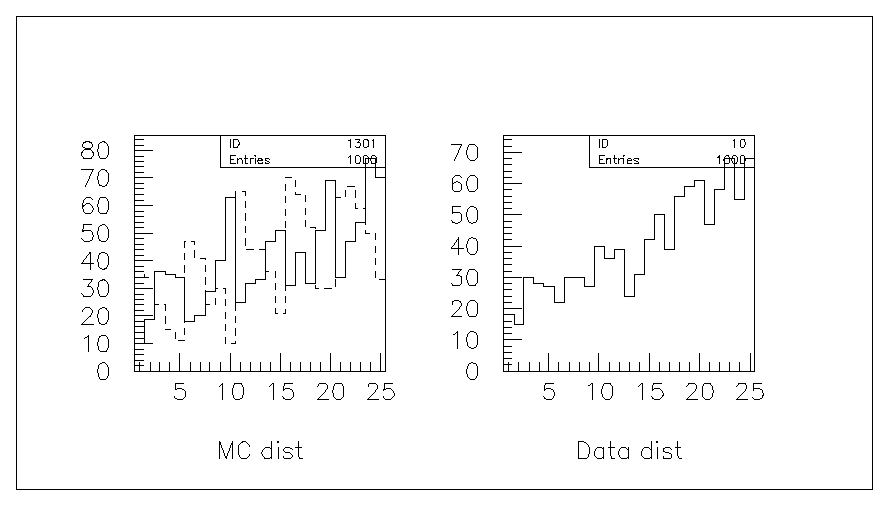
\epsfig{file=hmchis.eps,width=\the\textwidth}}
\end{center}
\caption{Monte Carlo distributions (left) and
data distribution (right).}
\label{Efield}
\end{figure}
%
\end{changebar}
 
\newpage%%%%%%%%%%%%%%%%%%%%%%%%%%%%%%%%%%%%%%%%%%%%%%%%%%%%%%%%%%

\subsection{Example of fits}

\begin{XMP}
      SUBROUTINE HEXAM5
*.==========>
*.           OPERATIONS ON HISTOGRAMS AND FITTING
*..=========> (R.Brun, modified by M.Goossens)
      COMMON/HFPAR/PAR(6)
      COMMON/HFGAUS/AG,BG,CG
      DOUBLE PRECISION AG,BG,CG
      DIMENSION X(100),Y(100)
      DIMENSION XF(4000,2),YF(4000),EY(4000),SIGPAR(6)
      DOUBLE PRECISION COV(6,6)
      EXTERNAL HFUNF,HFUNFV,HFUNGA
      CHARACTER*12 TITL1
      DATA TITL1/'TITLE OF ID1'/
*.___________________________________________
*
*             GET hist 110 from data base
*
      CALL HRGET(110,'hexam.dat',' ')
      CALL HRGET(210,'hexam.dat',' ')
*
*
      CALL HBOOK1(1,TITL1,100,0.,1.,0.)
      CALL HCOPY(1,2,'TITLE OF ID = 2')
*
*             Gets information from ID=110 and fills new IDs 1,2
*
      CALL HUNPAK(110,X,'HIST',1)
      CALL UCOPY(X,Y,100)
      CALL VZERO(X(51),50)
      CALL HPAK(1,X)
      CALL HPHIST(1,'HIST',1)
      CALL VZERO(Y,50)
      CALL HPAK(2,Y)
      CALL HPHIST(2,'HIST',1)
*
*             adds 1 and 2. Identifier 3 is created and will contain
*             result of addition
*
      CALL HOPERA(1,'+',2,3,1.,1.)
      CALL HCOPY(3,4,' ')
*
*             Fits 3 with function HFUNF, similar to example 2 .
*             Initializes parameters. Prints results of the last
*             iteration.
*             Superimpose result of fit to the histogram
*             The result of this fit can be compared with the initial
*             parameters of example 2
*
      PAR(1) = 40.
      PAR(2) = 20.
      PAR(3) = 0.4
      PAR(4) = 0.6
      PAR(5) = 0.1
      PAR(6) = 0.1
*
      CALL HFITH(3,HFUNF,'V',6,PAR(1),ST,PMI,PMA,SIGPAR,CHI2)
*
      CALL HPHIST(3,'HIST',1)
*
*
*            Fits a two-dimensional distribution (xf,yf) with HFITN
*            initialize parameters. Prints results of the last
*            iteration.
*            Errors EY automatically computed as SQRT(yf)
*
      NY=0
      DO 10 J=1,40
         DO 5 I=1,100
            CONT=HIJ (210,I,J)
            IF (CONT.EQ.0.) GOTO 5
            NY=NY+1
            YF(NY)=CONT
            EY(NY)=SQRT(CONT)
            CALL HIJXY (210,I,J,X1,X2)
            XF(NY,1)=X1+0.005
            XF(NY,2)=X2+0.0125
    5    CONTINUE
   10 CONTINUE
      PAR(1) = 3.
      PAR(2) = 1.
      PAR(3) = 0.3
      PAR(4) = 0.7
      PAR(5) = 0.07
      PAR(6) = 0.12
*
      CALL HFITV (NY,NY,1,XF,YF,EY,HFUNFV,'V',6,PAR(1),ST,PMI,PMA,
     +            SIGPAR,CHI2)
*       Get covariance matrix of last fit from Minuit.
*       Minuit parameters on 4-byte machines are Double precision 
      CALL MNEMAT(COV,6)
      WRITE(31,*) ' COVARIANCE MATRIX'
      WRITE(31,*) ' *****************'
      DO 20 I=1,6
        WRITE(31,'(6(D12.4,1X))') (COV(I,J),J=1,I)
   20 CONTINUE
*
*       Gaussian fit. Prints first and last iterations.
*
      AG = 2.
      BG = 0.4
      CG = 0.1
      CALL HDELET (0)
      CALL HBFUN1 (1,' ',100,0.,1.,HFUNGA)
      CALL HBOOK1 (5,' ',100,0.,1.,1000.)
      DO 30 I=1,5000
         XR=HRNDM1 (1)
         CALL HFILL (5,XR,0.,1.)
   30 CONTINUE
*
      PAR(1) = 200.
      PAR(2) = 0.4
      PAR(3) = 0.1
      CALL HFITHN(5,'G',' ',3,PAR(1),ST,PMI,PMA,SIGPAR,CHI2)
      CALL HPRINT (5)
      CALL HDELET (0)
*
      END
*
      FUNCTION HFUNF(X)
      COMMON/HFPAR/PAR(6)
      DOUBLE PRECISION A1,A2,C1,C2,XM1,XM2,XS1,XS2,X1,X2
*       Force double precision calculation
      C1  = PAR(1)
      C2  = PAR(2)
      XM1 = PAR(3)
      XM2 = PAR(4)
      XS1 = PAR(5)
      XS2 = PAR(6)
*
      A1=-0.5*((X-XM1)/XS1)**2
      A2=-0.5*((X-XM2)/XS2)**2
      IF(A1.LT.-20.)THEN
         X1=0.
      ELSEIF(A1.GT.20.)THEN
         X1=1.E5
      ELSE
         X1=C1*EXP(A1)
      ENDIF
      IF(A2.LT.-20.)THEN
         X2=0.
      ELSEIF(A2.GT.20.)THEN
         X2=1.E5
      ELSE
         X2=C2*EXP(A2)
      ENDIF
      HFUNF=X1+X2
      END
      FUNCTION HFUNFV (X)
      DIMENSION X(*)
*         Compute function value for 2-dim point X
      HFUNFV = HFUNF(X(1)) + HFUNF(X(2))
      END
      FUNCTION HFUNGA (X)
      COMMON/HFGAUS/AG,BG,CG
      DOUBLE PRECISION AG,BG,CG
      HFUNGA=AG*EXP(-0.5*((X-BG)/CG)**2)
      END
\end{XMP}
\newpage
\begin{Listing}
 TITLE OF ID1                                                                    
 
 HBOOK     ID =         1                                        DATE  18/05/92              NO =    14
 
      172                                    -
      168                                    I
      164                                    I
      160                                   -I
      156                                   II -
      152                                   II-I
      148                                   I  I-
      144                                 --I   I
      140                                 I     I-
      136                                 I      I
      132                                 I      I
      128                                 I      I-
      124                                -I       I
      120                               -I        I
      116                               I         I
      112                               I         I
      108                               I         I
      104                              -I         I-
      100                              I           I
       96                              I           I -
       92                              I           I-I
       88                             -I             I
       84                             I              I -
       80                             I              I I
       76                             I              I I
       72                             I              I I-
       68                             I              I-II
       64                             I                 I
       60                           - I                 I
       56                           I-I                 I
       52                           I                   I-
       48                          -I                    I-
       44                          I                      I
       40                          I                      I-
       36                          I                       I
       32                          I                       I    -
       28                         -I                       I- - I
       24                       --I                         I-I I
       20                      -I                             I I-
       16                      I                              I-II
       12                     -I                                 I
        8                 - --I                                  I
        4            -----I-I                                    I
 
 CHANNELS 100   0                                                                                                  1   
           10   0        1         2         3         4         5         6         7         8         9         0   
            1   1234567890123456789012345678901234567890123456789012345678901234567890123456789012345678901234567890   
 
 CONTENTS 100                          1111111111111                                                                
           10                 112224658012445755432099687543222121                                                  
            1.       211246268181476068282127104785115522257716498                                                  
 
 LOW-EDGE   1.            111111111122222222223333333333444444444455555555556666666666777777777788888888889999999999
 *10**  1   0   0123456789012345678901234567890123456789012345678901234567890123456789012345678901234567890123456789
 
 * ENTRIES =        100      * ALL CHANNELS = 0.2825E+04      * UNDERFLOW = 0.0000E+00      * OVERFLOW = 0.0000E+00
 * BIN WID = 0.1000E-01      * MEAN VALUE   = 0.3087E+00      * R . M . S = 0.7466E-01
 
\newpage

 TITLE OF ID = 2                                                                 
 
 HBOOK     ID =         2                                        DATE  18/05/92              NO =    15
 
       84                                                                               -
       82                                                                             - I
       80                                                                             I I
       78                                                                       -     I I  -
       76                                                                       I -   I I  I
       74                                                                       I-I  -I I  I
       72                                                                       I I  II I  I
       70                                                                       I I- II I  I -
       68                                                                       I  I II-I -I-I
       66                                                                    -  I  I-I  I-I  I
       64                                                                  - I  I            I-
       62                                                                  I-I  I             I
       60                                                                  I I -I             I
       58                                                                  I I I              I
       56                                                                  I I I              I
       54                                                                  I I-I              I -
       52                                                                - I                  I I
       50                                                                I-I                  I-I
       48                                                                I                      I
       46                                                                I                      I
       44                                                                I                      I   -
       42                                                               -I                      I-  I
       40                                                              -I                        I  I
       38                                                              I                         I  I
       36                                                              I                         I  I-
       34                                                              I                         I--II
       32                                                              I                             I
       30                                                             -I                             I
       28                                                         -   I                              I  -
       26                                                         I  -I                              I- I
       24                                                         I  I                                I I
       22                                                         I- I                                I I--
       20                                                         II I                                I-I I -
       18                                                         II-I                                    I I
       16                                                         I                                       I-I
       14                                                         I                                         I
       12                                                         I                                         I--
       10                                                         I                                           I
        8                                                         I                                           I - -
        6                                                         I                                           I-I-I
        4                                                         I                                               I-
        2                                                         I                                                I
 
 CHANNELS 100   0                                                                                                  1   
           10   0        1         2         3         4         5         6         7         8         9         0   
            1   1234567890123456789012345678901234567890123456789012345678901234567890123456789012345678901234567890   
 
 CONTENTS  10                                                     221233455666557776678686676664543343222221111     
            1.                                                    71850922032539736953183588893942434650812591167574
 
 LOW-EDGE   1.            111111111122222222223333333333444444444455555555556666666666777777777788888888889999999999
 *10**  1   0   0123456789012345678901234567890123456789012345678901234567890123456789012345678901234567890123456789
 
 * ENTRIES =        100      * ALL CHANNELS = 0.2175E+04      * UNDERFLOW = 0.0000E+00      * OVERFLOW = 0.0000E+00
 * BIN WID = 0.1000E-01      * MEAN VALUE   = 0.7102E+00      * R . M . S = 0.1063E+00
\newpage
{\scriptsize
  MINUIT RELEASE 90.10  INITIALIZED.   DIMENSIONS 100/ 50  EPSMAC=  0.89E-15
 **********
 **    1 **SET EPS  0.1000E-06
 **********
 FLOATING-POINT NUMBERS ASSUMED ACCURATE TO   0.100E-06

     **********************************************
     *                                            *
     * Function minimization by SUBROUTINE HFITH  *
     * Variable-metric method                     *
     * ID =          3  CHOPT = V                 *
     *                                            *
     **********************************************
 Convergence when estimated distance to minimum (EDM) .LT.  0.10E-03

 PARAMETER DEFINITIONS:
    NO.   NAME         VALUE      STEP SIZE      LIMITS
     1 'P1        '    40.000       12.000         no limits
     2 'P2        '    20.000       6.0000         no limits
     3 'P3        '   0.40000      0.12000         no limits
     4 'P4        '   0.60000      0.18000         no limits
     5 'P5        '   0.10000      0.30000E-01     no limits
     6 'P6        '   0.10000      0.30000E-01     no limits
 **********
 **    2 **SET PRINT  0.0000    
 **********
 **********
 **    3 **MIGRAD   1160.       1.000    
 **********

 MIGRAD MINIMIZATION HAS CONVERGED.

 MIGRAD WILL VERIFY CONVERGENCE AND ERROR MATRIX.

 FCN=   81.55959     FROM MIGRAD    STATUS=CONVERGED    391 CALLS      392 TOTAL
                     EDM=  0.21E-05    STRATEGY= 1      ERROR MATRIX ACCURATE 

  EXT PARAMETER                                   STEP         FIRST   
  NO.   NAME        VALUE          ERROR          SIZE      DERIVATIVE 
   1      P1        154.37        3.8591       0.97447      -0.16735E-03
   2      P2        74.934        2.1210       0.51925       0.16237E-03
   3      P3       0.30351       0.15347E-02   0.76783E-03  -0.91430    
   4      P4       0.70017       0.29587E-02   0.17713E-02   0.19339    
   5      P5       0.69299E-01   0.12334E-02   0.28758E-03   0.39057    
   6      P6       0.11985       0.27357E-02   0.62656E-03   0.52392    

 CHISQUARE = 0.9164E+00  NPFIT =   95
}
\newpage
 
 TITLE OF ID1                                                                    
 
 HBOOK     ID =         3                                        DATE  18/05/92              NO =    16
 
      172                                    -
      168                                    I
      164                                    I
      160                                   -I
      156                                   I***
      152                                   *I-I
      148                                   I  I*
      144                                 -*I   I
      140                                 I     I*
      136                                 *      I
      132                                 I      I*
      128                                 I      I-
      124                                *I       I
      120                               -I        I*
      116                               I         I
      112                               *         I
      108                               I         I *
      104                              -I         I-
      100                              I           I
       96                              *           I *
       92                              I           I-I
       88                             -I             I
       84                             *              I -                              - -
       80                             I              I*I                        -     I I  -
       76                             I              I I                        I--******  I
       72                            *I              I I-                       I**- II I**I -
       68                             I              I-*I                    - **  I-II-I--**I
       64                             I                 I                  --I* I            *-
       60                           * I                 *                  I * -I             *
       56                           I-I                 I                  I*I-I              I*-
       52                           I                   I-               --*                  I-*
       48                          *I                    *-              I*                     I*
       44                          I                      I             -*                      I-* -
       40                          I                      *-           **                        I **
       36                         *I                       I          *I                         I--I*
       32                          I                       *    -    *-I                             I*
       28                        *-I                       I* - I -**-I                              I-*-
       24                       *-I                         I***I**- I                                I *--
       20                      -I                             I *-II-I                                I-I** -
       16                      *                              I-I                                         I**
       12                    **I                                                                            I**
        8                 - *-I                                                                               I****
        4       ************I                                                                                     I*
 
 CHANNELS 100   0                                                                                                  1   
           10   0        1         2         3         4         5         6         7         8         9         0   
            1   1234567890123456789012345678901234567890123456789012345678901234567890123456789012345678901234567890   
 
 CONTENTS 100                          1111111111111                                                                
           10                 112224658012445755432099687543222121221233455666557776678686676664543343222221111     
            1.       21124626818147606828212710478511552225771649871850922032539736953183588893942434650812591167574
 
 LOW-EDGE   1.            111111111122222222223333333333444444444455555555556666666666777777777788888888889999999999
 *10**  1   0   0123456789012345678901234567890123456789012345678901234567890123456789012345678901234567890123456789
 
 * ENTRIES =        200      * ALL CHANNELS = 0.5000E+04      * UNDERFLOW = 0.0000E+00      * OVERFLOW = 0.0000E+00
 * BIN WID = 0.1000E-01      * MEAN VALUE   = 0.4834E+00      * R . M . S = 0.2184E+00
 * CHISQUAR  =  0.8156E+02
\newpage
{\scriptsize
     **********************************************
     *                                            *
     * Function minimization by SUBROUTINE HFITV  *
     * Variable-metric method                     *
     * ID =          0  CHOPT = V                 *
     *                                            *
     **********************************************
 Convergence when estimated distance to minimum (EDM) .LT.  0.10E-03

 PARAMETER DEFINITIONS:
    NO.   NAME         VALUE      STEP SIZE      LIMITS
     1 'P1        '    3.0000      0.90000         no limits
     2 'P2        '    1.0000      0.30000         no limits
     3 'P3        '   0.30000      0.90000E-01     no limits
     4 'P4        '   0.70000      0.21000         no limits
     5 'P5        '   0.70000E-01  0.21000E-01     no limits
     6 'P6        '   0.12000      0.36000E-01     no limits
 **********
 **    4 **SET PRINT  0.0000    
 **********
 **********
 **    5 **MIGRAD   1160.       1.000    
 **********
 MACHINE ACCURACY LIMITS FURTHER IMPROVEMENT.

 MIGRAD MINIMIZATION HAS CONVERGED.

 MIGRAD WILL VERIFY CONVERGENCE AND ERROR MATRIX.
 EIGENVALUES OF SECOND-DERIVATIVE MATRIX:
        -0.1596E+01 -0.6458E+00  0.3800E+00  0.7478E+00  0.1277E+01  0.5837E+01
 MINUIT WARNING IN HESSE   
 ============== MATRIX FORCED POS-DEF BY ADDING   1.6018     TO DIAGONAL.
 MIGRAD TERMINATED WITHOUT CONVERGENCE.

 FCN=   1709.709     FROM MIGRAD    STATUS=FAILED       197 CALLS      198 TOTAL
                     EDM=  0.41E+02    STRATEGY= 1      ERR MATRIX NOT POS-DEF

  EXT PARAMETER                APPROXIMATE        STEP         FIRST   
  NO.   NAME        VALUE          ERROR          SIZE      DERIVATIVE 
   1      P1        2.4709       0.73263E-01   0.00000        4.1109    
   2      P2        1.8247       0.37237E-01   0.00000        8.5400    
   3      P3       0.27725       0.24789E-02   0.00000       -125.59    
   4      P4       0.70933       0.51778E-02   0.00000        132.72    
   5      P5       0.90472E-01   0.47875E-02   0.00000       -302.38    
   6      P6       0.21181       0.75383E-02   0.00000       -63.830    

 CHISQUARE = 0.9282E+00  NPFIT = 1848

  COVARIANCE MATRIX
  *****************
  0.5367E-02 
  0.9472E-03   0.1387E-02 
  0.4548E-05  -0.9488E-06   0.6145E-05 
 -0.1520E-04  -0.2581E-04   0.1647E-05   0.2681E-04 
 -0.2597E-03  -0.7556E-04  -0.2361E-06   0.2208E-05   0.2292E-04 
  0.1100E-03  -0.3230E-04  -0.1566E-05   0.1904E-05  -0.2129E-04   0.5683E-04 

     **********************************************
     *                                            *
     * Function minimization by SUBROUTINE HFITH  *
     * Variable-metric method                     *
     * ID =          5  CHOPT =                   *
     *                                            *
     **********************************************
 Convergence when estimated distance to minimum (EDM) .LT.  0.10E-03

 FCN=   69.87250     FROM MIGRAD    STATUS=CONVERGED     64 CALLS       65 TOTAL
                     EDM=  0.38E-05    STRATEGY= 1      ERROR MATRIX ACCURATE 

  EXT PARAMETER                                   STEP         FIRST   
  NO.   NAME        VALUE          ERROR          SIZE      DERIVATIVE 
   1      P1        199.30        3.5192       0.84934      -0.13509E-03
   2      P2       0.39761       0.14150E-02   0.10059E-02   -1.6362    
   3      P3       0.98783E-01   0.10313E-02   0.24990E-03   -1.7442    

 CHISQUARE = 0.1075E+01  NPFIT =   68
}



 EXAMPLE NO = 5                                                                  
 --------------                                                                  
 
                                                                                 
 
 HBOOK     ID =         5                                        DATE  18/05/92              NO =    17
 
      230                                               -
      220                                            -  I
      210                                            I  I
      200                                            ****** -
      190                                          **I  I--*I-
      180                                         *I I    I *I
      170                                        * I-I    I-I*
      160                                       *I-I         I*
      150                                      *I             I*
      140                                      -I              I*
      130                                    -*I               I *--
      120                                    *-I               I--*I
      110                                   *I                     I
      100                                  *I                      *-
       90                                 *I                        *
       80                                *I                         I*
       70                               *I                          I-*
       60                              *-I                           I *--
       50                             *-I                            I-I*I
       40                           -*I                                  **-
       30                         -**                                    I-**
       20                       ***                                        I-***
       10       ****************I                                              I************************************
 
 CHANNELS 100   0                                                                                                  1   
           10   0        1         2         3         4         5         6         7         8         9         0   
            1   1234567890123456789012345678901234567890123456789012345678901234567890123456789012345678901234567890   
 
 CONTENTS 100                               111111111211211121111111                                                
           10                 1 112233456889131356586199288608541122964655231111                                    
            1.    1    2224268062313614000760053587389243868095597245890427768955738341  11        1                
 
 LOW-EDGE   1.            111111111122222222223333333333444444444455555555556666666666777777777788888888889999999999
 *10**  1   0   0123456789012345678901234567890123456789012345678901234567890123456789012345678901234567890123456789
 
 * ENTRIES =       5000      * ALL CHANNELS = 0.5000E+04      * UNDERFLOW = 0.0000E+00      * OVERFLOW = 0.0000E+00
 * BIN WID = 0.1000E-01      * MEAN VALUE   = 0.3984E+00      * R . M . S = 0.9985E-01
 * CHISQUAR  =  0.6987E+02
\end{Listing}
\newpage
\begin{XMPt}{Example of parametrization and smoothing}
      SUBROUTINE HEXAM6
*.==========>
*.           PARAMETRIZATION      -     SMOOTHING
*..=========> ( R.Brun )
      DOUBLE PRECISION COEFF
      DIMENSION ITERM(15),COEFF(15)
*.___________________________________________
*
*             Get hist 110 from data base
*
      CALL HRGET(110,'hexam.dat',' ')
*
*       Find best parametrization of histogram in terms of powers
*       of shifted Tchebychev polynomials
*       also produces the corresponding fortran function (here on
*       standard output)
*
*
      CALL HCOPY(110,1,' ')
      CALL HSETPR('PNBX',15.)
      CALL HSETPR('PNCX',15.)
      CALL HSETPR('PLUN',31.)
      CALL HPARAM(1,3011,1.,14,COEFF,ITERM,NCO)
      CALL HPRINT(1)
*
*        ID=2 is smoothed with B-splines
*        statistical errors (sqrt of contents) are drawn
*
      CALL HCOPY(110,2,' ')
      CALL HSPLI1(2,2,14,3,CHI2)
      CALL HIDOPT(2,'ERRO')
      CALL HPHIST(2,'HIST',1)
      END
\end{XMPt}
\newpage
\begin{Listing}
{\scriptsize

 ****************************************
 *                                      *
 *   MULTIDIMENSIONAL PARAMETRIZATION   *
 *                                      *
 ****************************************

 FIT CHARACTERISTICS AND OPTIONS
 *******************************

 ID =   1
 DIM =  1
 WORKING SPACE IN /PAWC/ =    5045
  0 USER-DEFINED BASIC FUNCTIONS
  0 USER-DEFINED ELEMENTARY FUNCTIONS
 MAX NUMBER OF REGRESSORS = 15
 MAX POWERS OF POLYNOMIALS IN  EACH DIM = 14  
 AMOUNT OF OUTPUT = 1
 WEIGHTING TYPE = 0
 CLASS OF POLYNOMIALS = 3
 CLASS OF BASIC FUNCTIONS = 0
 BASIC FUNCTION SELECTION MODE = 0
 REGRESSION MODE = 0
 X-NORMALIZATION TYPE = 0
 POWER LIMITOR =  1.00
 F-TEST LEVEL =   1.00
 PARAMETRIZATION SUPERIMPOSED ON HISTOGRAM
 FORTRAN CODE FPARAM WRITTEN ON UNIT 31

 FITTING PROCESS WILL STOP WHEN THE RESIDUAL VARIANCE HITS A MINIMUM

  15 CANDIDATE BASIC FUNCTIONS WERE RETAINED FOR THE FIT
 NUMBER OF POINTS TO FIT =    95
 SUM OF SQUARES OF Y-VALUES =   5000.0    
 MACHINE PRECISION =  0.22E-15


 FITTING PROCESS STOPPED AS RESIDUAL VARIANCE HITS MINIMUM
 R2 =  0.98543      12 REGRESSORS INCLUDED

 FINAL RESULTS OF THE FIT
 ************************

 ITERATION       RSS       R2ADJ     REGRESSOR  COEFF. VALUE   TERM OF PARAMETRIZATION

    13        72.841       0.98350       1        40.320         0 
                                         2       -32.156        20 
                                         3        29.461        60 
                                         4       -20.018        80 
                                         5        7.7912       100 
                                         6       -18.482        50 
                                         7       -7.0469       110 
                                         8       -9.0691        10 
                                         9        4.4675       130 
                                        10        6.4382        90 
                                        11       -3.9874       140 
                                        12        3.1189        30 

 REGRESSOR  STANDARD DEVIATION     CONFIDENCE INTERVAL
     1          0.70650         [  39.144    ,  41.495    ]
     2           1.0509         [ -33.904    , -30.407    ]
     3          0.85147         [  28.044    ,  30.877    ]
     4          0.90853         [ -21.530    , -18.506    ]
     5          0.82336         [  6.4213    ,  9.1611    ]
     6           1.0259         [ -20.189    , -16.775    ]
     7          0.78401         [ -8.3514    , -5.7425    ]
     8           1.0731         [ -10.854    , -7.2836    ]
     9          0.68036         [  3.3355    ,  5.5995    ]
    10          0.83660         [  5.0463    ,  7.8301    ]
    11          0.85716         [ -5.4135    , -2.5612    ]
    12           1.1372         [  1.2267    ,  5.0110    ]
      DOUBLE PRECISION FUNCTION FPARAM (X)
      DOUBLE PRECISION COEFF,P,P0,P1,P2,HELEFT,HBASFT
      DIMENSION X(1),COEFF(12),IBASFT( 1,12)
      DATA COEFF/ 0.40319615E+02,-0.32155589E+02, 0.29460772E+02,
     +-0.20017895E+02, 0.77912196E+01,-0.18481896E+02,
     +-0.70469122E+01,-0.90690550E+01, 0.44674803E+01,
     + 0.64381900E+01,-0.39873663E+01, 0.31188760E+01
     +/
      DATA IBASFT/  0, 20, 60, 80,100, 50,110, 10,130, 90,140, 30
     +/
      FPARAM=0.
      DO 25 K=1,12
      P=1.
      DO 15 I=1, 1
      NUM=IBASFT(I,K)/10
      ITYP=IBASFT(I,K)-NUM*10
      IF (NUM.NE.0) THEN
      IF (ITYP.EQ.0) THEN
      P0=1.
      P1=2*X (I)-1.
      DO 10 J=2,NUM
      P2=2*(2*X (I)-1.)*P1-P0
      P0=P1
   10 P1=P2
      P=P*P1
      END IF
      IF (ITYP.EQ.1) P=P*HELEFT(NUM,X (I))
      IF (ITYP.EQ.2) THEN
      P=HBASFT(NUM,X )
      GOTO 20
      END IF
      END IF
   15 CONTINUE
   20 FPARAM=FPARAM+COEFF(K)*P
   25 CONTINUE
      RETURN
      END
}
\newpage
 THIS HISTOGRAM IS FILLED ACCORDING TO THE FUNCTION HTFUN1                       

 HBOOK     ID =         1                                        DATE  17/12/91              NO =  18
 
      172                                    -
      168                                    I
      164                                    I
      160                                   -I
      156                                   II -
      152                                   I**I
      148                                   *  *-
      144                                 -*I   *
      140                                 I     I-
      136                                 *      *
      132                                 I      I
      128                                *I      I*
      124                                -I       I
      120                               -I        I*
      116                               *         I
      112                               I         I
      108                               I         I *
      104                              -I         I-
      100                              *           I
       96                              I           I *
       92                              I           I-I
       88                             *I             I
       84                             I              I*-                              - -
       80                             I              I I                        -     I I  -
       76                            *I              I I                        I-******** I
       72                             I              I *-                       **I- II I *I -
       68                             I              I-II                    - *I  I-II-I--**I
       64                             I                 I                  --I* I            *-
       60                           * I                 *                  I** -I             *
       56                           I-I                 I                  * I-I              I*-
       52                           I                   I*               -*I                  I-*
       48                          *I                    I-              *                      I*
       44       *                  I                      *             *I                      I-* -
       40                          I                      I-           *I                        I *I
       36        *                *I                       *          *I                         I--*-
       32                          I                       I    -    *-I                             **
       28                        *-I                       I* - I - *-I                              I-*-
       24         *             --I                         I*I I ** I                                I **-
       20                      -*                             ****II-I                                I-I **-
       16          *           *                              I-I                                         I-**
       12                     *I                                                                            I-*
        8           *     -***I                                                                               I****
        4            ******-I                                                                                     I*
 
 CHANNELS 100   0                                                                                                  1   
           10   0        1         2         3         4         5         6         7         8         9         0   
            1   1234567890123456789012345678901234567890123456789012345678901234567890123456789012345678901234567890   
 
 CONTENTS 100                          1111111111111                                                                
           10                 112224658012445755432099687543222121221233455666557776678686676664543343222221111     
            1.       21124626818147606828212710478511552225771649871850922032539736953183588893942434650812591167574
 
 LOW-EDGE   1.            111111111122222222223333333333444444444455555555556666666666777777777788888888889999999999
 *10**  1   0   0123456789012345678901234567890123456789012345678901234567890123456789012345678901234567890123456789
 
 * ENTRIES =       5000      * ALL CHANNELS = 0.5000E+04      * UNDERFLOW = 0.0000E+00      * OVERFLOW = 0.0000E+00
 * BIN WID = 0.1000E-01      * MEAN VALUE   = 0.4834E+00      * R . M . S = 0.2184E+00
 * CHISQUAR  =  0.7284E+02

\newpage
 
 THIS HISTOGRAM IS FILLED ACCORDING TO THE FUNCTION HTFUN1                       
 
 HBOOK     ID =         2                                        DATE  17/12/91              NO =  19
 
      185                                    I
      180                                    I
      175                                    0
      170                                   II I
      165                                   IIII
      160                                   0IIII
      155                                 III I0I
      150                                 III**I0I
      145                                 00* I*II
      140                                 I*  I *0I
      135                                I*I    III
      130                               III      *I
      125                               I*        *
      120                               0I        I
      115                              I*I        I*
      110                              II          I
      105                              0           0*I
      100                             I*           III
       95                             II           I0* I                                I
       90                             *             II I                        I     I I  I
       85                             I             I *0I                       III  I0 0  I
       80                            *I                II                       0I0I***II I0II
       75                                             I*0                  I I  ****I0I***IIIII
       70                           *                 I I                  III**III0II 0 I**00I
       65                           II                0 *                  00*II I I0I I 0I **0 I
       60                           00                I  *               III*II0    I  I II I *II
       55                          *II                   0I              0I*I 0I               **   I
       50                          0 I                   I*            III*   I                0I*  I
       45                         *I                     I0*           I**I                    I 0* 0I
       40                          I                      I0          I*I                        II**0
       35                        *I                        I* I I I   *I                          00 *  I
       30                       II0                         0** 0 0I**0                           II I**0II
       25                      I*0I                         I0I*****I0I                               0I**0 I
       20                      *II                           I I 0 I0I                                I0 I**0
       15                    I*I                               0 I  I                                      0**0
       10                I0 0*I                                                                              I****0I
        5            ********                                                                                  II0**
 
 CHANNELS 100   0                                                                                                  1   
           10   0        1         2         3         4         5         6         7         8         9         0   
            1   1234567890123456789012345678901234567890123456789012345678901234567890123456789012345678901234567890   
 
 CONTENTS 100                          1111111111111                                                                
           10                 112224658012445755432099687543222121221233455666557776678686676664543343222221111     
            1.       21124626818147606828212710478511552225771649871850922032539736953183588893942434650812591167574
 
 LOW-EDGE   1.            111111111122222222223333333333444444444455555555556666666666777777777788888888889999999999
 *10**  1   0   0123456789012345678901234567890123456789012345678901234567890123456789012345678901234567890123456789
 
 * ENTRIES =       5000      * ALL CHANNELS = 0.5000E+04      * UNDERFLOW = 0.0000E+00      * OVERFLOW = 0.0000E+00
 * BIN WID = 0.1000E-01      * MEAN VALUE   = 0.4834E+00      * R . M . S = 0.2184E+00
 * CHISQUAR  =  0.9674E+02
\end{Listing}
\index{fitting Monte Carlo statistics|)}
\index{Monte Carlo statistics|)}

\endinput

 
 
\section{Fitting with finite Monte Carlo statistics}
\index{maximum likelihood}
\index{likelihood}
\index{test!Monte Carlo distribitions}
 
The following three routines are intended to help with problems of the 
type: 
\begin{quote}
``Given a data distribution, and a set of Monte Carlo distributions,
what is the best estimate of the fraction of each Monte Carlo distribution
present in the data distribution?.''
\end{quote}
An example is the determination of
the proportions of different sources (direct b decay, cascade b decays,
c decays, background) contributing to the spectrum of
inclusive leptons in Z decay events).
 
The maximum likelihood method is used,
the likelihood function being calculated including the effect of both data and
Monte Carlo statistics, as described in ~\cite{bib-FINITEMC}.  
Subroutine
\Rind{HMCMLL} uses \MINUIT{} to perform the log-likelihood maximisation and 
return a set of fractions.  
Functions \Rind{HMCINI} and \Rind{HMCLNL} are 
provided for those who wish to perform the fit themselves. 
 
\fbox{\parbox{.96\textwidth}{%
Note that all floating point parameters and functions are 
of type \Lit{REAL*8} (double precision on most machines).}}
 
\newpage%%%%%%%%%%%%%%%%%%%%%%%%%%%%%%%%%%%%%%%%%%%%%%%%%%%%

\Shubr{HMCMLL}{(IDD,IDM,IDW,NSRC,CHOPT,IFIX,FRAC,FLIM,START,
                STEP,UP,PAR*,DPAR*)}
 
\Action
Fits the given Monte Carlo distributions to the data distribution, using
a binned maximum likelihood fit which includes the effect of both data and 
Monte Carlo statistics, and allows weights to be 
provided for each Monte Carlo distribution.  The data and Monte Carlo
distributions must be presented in 1 dimensional histograms.  
The best estimate of the fraction of each Monte 
Carlo distribution present in the data distribution is returned, with an
error estimate where required.
 
\begin{DLtt}{12345}
\item[{\rm\bf Input parameters:}]
\item[IDD] Data histogram identifier.
\item[IDM] Array of dimension \Lit{NMCSRC} containing Monte Carlo histogram 
           identifiers.
\item[IDW] Array of dimension \Lit{NMCSRC} containing weight histogram 
           identifiers. (\Lit{'W'} option only).
\item[NSRC] Number of Monte Carlo sources.  Must be greater than 1.
\item[CHOPT] character variable specifying the desired options.
\begin{DLtt}{123}
\item['E'] Perform a detailed error analysis using the MINUIT routines
           \Rind{HESSE} and \Rind{MINOS}. 
\item['F'] Fix one or more of the fractions.  Default is for all fractions
           to vary freely.
\item['L'] Set limits on the fractions as given in \Lit{FLIM}.  Default 
           is no limits.
\item['N'] Do not perform the fit.
\item['P'] Use the parameter start points and initial step sizes provided 
           in \Lit{START} and \Lit{STEP}. 
           If the \Lit{'P'} option is
           not specified then the start point for each free parameter is
           $\frac{\textstyle 1 - \Sigma_{f}}{\textstyle\mathtt{NSRC}-N_{f}}$, 
           where $\Sigma_{f}$ is the sum of the fixed fractions, and 
           $N_{f}$ is the number of fixed fractions; 
           and the initial step size is 0.01.
\item['S'] Scan the likelihood function with respect to each fit parameter,
           before and after the fit.  
           If the \Lit{'N'} option is specified, the function 
           will only be scanned once for each parameter.
\item['W'] Use the weight histograms provided.  For non existent weight 
           histograms, and if the W option is not requested, a dummy 
           weight histogram in which all entries are 1 is booked.
\end{DLtt}
\item[IFIX] Double Precision array of dimension \Lit{NMCSRC} containing \Lit{'1'} if a 
            parameter is to be fixed in the fit, \Lit{'0'} otherwise
            (\Lit{'F'} option only).
\item[FRAC] Double precision array of dimension \Lit{NMCSRC} with the values at which
            parameters are to be fixed (\Lit{'F'} option only).
\item[FLIM] Double precision array of dimension \Lit{(2,NMCSRC)} with the lower, then
            upper limits on the parameters (\Lit{'L'} option only.)
\item[START] Double precision array of dimension \Lit{NMCSRC} with the start values for
            each parameter (\Lit{'P'} option only).
\item[STEP] Double precision array of dimension \Lit{NMCSRC} with initial step values for each
            parameter (\Lit{'P'} option only).
\item[UP]   \Lit{UP} value for the error estimate (\Lit{'E'} option only).  
            A default value of 0.5 is taken when you specify \Lit{UP\(\leq\)0}
            and use the \Lit{'E'} option
            (see the \MINUIT{} manual for the definition of \Rarg{UP}).
\item[{\rm\bf Output parameters:}]
\item[PAR]  Double precision array of dimension \Lit{NMCSRC} with the final fitted values
            of the parameters.
\item[DPAR] Double precision array of dimension \Lit{NMCSRC} with the errors
            on the final fitted values of the parameters.
\end{DLtt}
 
 
\newpage%%%%%%%%%%%%%%%%%%%%%%%%%%%%%%%%%%%%%%%%%%%%%%%%%%%%%%%%%%%
 
\Shubr{HMCINI}{(IDDATA,IDMC,IDWT,NSRC,CHOPT,IERR)}
 
\Action
Initialisation routine for function \Rind{HMCLNL}, needs to be called
each time a new set of histograms is introduced (generally once at the
beginning of each fit). 
Performs some error checking and sets up a dummy 
weight histogram if necessary.
 
\begin{DLtt}{12345}
\item[{\rm\bf Input parameters:}]
\item[IDDATA] Data histogram identifier.
\item[IDMC]   Array of dimension \Lit{NMCSRC} containing Monte Carlo histogram 
              identifiers.
\item[IDWT]   Array of dimension \Lit{NMCSRC} containing weight histogram 
              identifiers. (\Lit{'W'} option only).
\item[NMCSRC] Number of Monte Carlo sources.
\item[CHOPT]  Character variable specifying the selected options.
    \begin{DLtt}{123}
      \item[' '] Default. A dummy weight histogram is booked 
                 in which all entries are 1.
      \item['W'] Use the weight histograms provided.  
                 If no weight histograms exist, proceed as for the default above.
    \end{DLtt}
\item[IERR]   Error flag - set to 1 if the parameters sent to \Rind{HMCINI}
              were not usable 
              (e.g., incompatibility between data and MC histograms, 
              number of MC sources less than 2), 0 otherwise.
\end{DLtt}
 
\Sfunc{HMCLNL}{VARIAB = HMCLNL(FRAC)}
 
\Action
\Rind{HMCLNL} is a double precision function giving the log likelihood 
(including effect of both data
and Monte Carlo statistics) that the data distribution arose from a
distribution given by combining the Monte Carlo distributions, weighted
by the weights provided, using the fractions given in \Rarg{FRAC}.
\Rind{HMCINI} must be called before this function may be used.
 
\begin{DLtt}{12345}
\item[{\rm\bf Input parameters:}]
\item[FRAC] Double precision array of dimension \Lit{NMCSRC} containing the 
            fraction of each Monte Carlo distribution you wish to assume is 
            in the data distribution, in order to calculate the log likelihood.
\end{DLtt}


% Local Variables: 
% mode: latex
% TeX-master: "hboomain"
% End: 

%%%%%%%%%%%%%%%%%%%%%%%%%%%%%%%%%%%%%%%%%%%%%%%%%%%%%%%%%%%%%%%%%%%
%                                                                 %
%   HBOOK User Guide -- LaTeX Source                              %
%                                                                 %
%   Chapter 8                                                     %
%                                                                 %
%   The following external EPS files are referenced:              %
%           pawstor.eps, hbzebra.eps                              %
%                                                                 %
%   Editor: Michel Goossens / CN-AS                               %
%   Last Mod.: 17 Feb 1995 21:45 mg                               %
%                                                                 %
%%%%%%%%%%%%%%%%%%%%%%%%%%%%%%%%%%%%%%%%%%%%%%%%%%%%%%%%%%%%%%%%%%%
 
\Filename{H1Memory-Management-and-IO-Routines}
\chapter{Memory Management and input/output Routines}
\label{HMEMORYM}
 
\Filename{H2Memory-usage-and-ZEBRA}
\section{Memory usage and ZEBRA}
\label{HMEMOUSE}

The \HBOOK{} system uses the \ZEBRA{} data manager
to store its data elements in a COMMON block \Lit{/PAWC/} 
(shared with the \KUIP{} and \HIGZ{} packages, when the latter are
also used, as is the case in \PAW{}). In fact the first task of a
\index{data structure}
\HBOOK{} user is to declare the length of this common to
\ZEBRA{} by a call to \Rind{HLIMIT}, as is seen in
figures \ref{FEX1IN} and \ref{FEX2IN}
      
In the \Lit{/PAWC/} data store, the \HBOOK,
\HIGZ{} and \KUIP{} packages have all their own
{\bf division} (see \cite{bib-ZEBRA} for
more details on the notion of divisions) as follows (see figure \ref{FPAWSTOR}):
 
\begin{DLtt}{12345}
\item[LINKS] Some locations at the beginning of
      \Lit{/PAWC/}
      \index{common {\tt/PAWC/}}\index{PAWC@{\tt/PAWC/} common}
      for \ZEBRA{} pointers.
\item[WORKS]  Working space (or division \Lit{1}) used by the
      various packages storing information in \Lit{/PAWC/}
\item[HBOOK] Division \Lit{2} of the store. Reserved to \HBOOK.
\item[HIGZ] A division reserved for the \HIGZ{} graphics package.
      This division only exists when \HIGZ{} is called.
\item[KUIP] A division reserved for the \KUIP{} user interface package.
      This division only exists when \KUIP{} is called.
\item[SYSTEM] The \ZEBRA{} system division.
      It contains some tables, as well as
      the Input/Output buffers for \Rind{HRIN} and \Rind{HROUT}.
\end{DLtt}

\begin{Fighere}
\begin{verbatim}
      COMMON/PAWC/NWPAW,IXPAWC,IHDIV,IXHIGZ,IXKU,FENC(5),LMAIN,HCV(9989)
      DIMENSION IQ(2),Q(2),LQ(8000)
      EQUIVALENCE (LQ(1),LMAIN),(IQ(1),LQ(9)),(Q(1),IQ(1))
\end{verbatim}
\begin{center}
\mbox{\epsfig{file=pawstor.eps,width=\the\textwidth}}
\end{center}
\caption{The layout of the \protect\Lit{/PAWC/} dynamic store}
\label{FPAWSTOR}
\end{Fighere}

\subsection{The use of ZEBRA}
     
Inside the \HBOOK{} division the various data elements are
stored as a \ZEBRA{} data structure, one for each ``identifier''.
In fact all identifiers (histogram or Ntuple numbers)
are stored in an ordered array in a \ZEBRA{}
bank and access to the information associated with the \HBOOK{} data
is via the {\bf reference link} at the same offset as the
identifier in the data part of the bank. The data structure for
a given element depends on its characteristics.
In any case the top bank for a given element contains the
title and other constants, while the data themselves are
stored in another bank hanging from the previous one. Sometimes
other banks are created, e.g. for automatic binning,
for storing the limits of the elements of a Ntuple and,
when a Ntuple is kept in memory, for containing the overflow
\index{projection}
of the data, for {\bf projections}, {\bf slices} and
\index{band}
{\bf bands} in the 2-dim case of for containing the {\bf errors}
\index{error}
associated to a bin. This means that each \HBOOK{} identifier
has a whole set of {\bf attributes} associated with its
\index{attribute}
existence, and when a histogram or Ntuple is written to backup
store and later reread, the {\bf complete data structure}, containing
all characteristics and attributes are retrieved.
Figure \ref{FZEBRA} shows
the \ZEBRA{} data structure for a two-dimensional histogram.
The precise layout of this bank should be of no concern to the
user. It is only shown here as an example of the underlying \ZEBRA{} structure
of \HBOOK. Note the use of the {\bf data} part of the bank for
storing attributes (e.g. title, number of bins, number of entries) as
well as of the {\bf link} part for storing the addresses to access the
associated data points (scatter plot contents, X and Y projections,
slices and bands and their associated errors).

\begin{figure}[p]
\caption[The ZEBRA data structure used for two-dimensional histograms]%
        {The \ZEBRA{} data structure used for two-dimensional histograms}
\label{FZEBRA}
\begin{center}
\mbox{\epsfig{file=hbzebra.eps,width=\the\textwidth}}
\end{center}
\end{figure}

\Filename{H2Memory-size-control}
\section{Memory size control}
\label{HMEMORYS}
 
\Shubr{HLIMIT}{(NWPAW)}
 
\Action
Defines the maximum total size \Lit{NWPAW}  of common
\Lit{/PAWC/}.
 
\Remark
\begin{UL}
\item \Rind{HLIMIT} must be called before any other \HBOOK{}
routine.
\item \HBOOK{} is compiled with a \Lit{COMMON/PAWC/} dimensioned to \Lit{10000} words.
If \Lit{NWPAW<10000}, then the default value of \Lit{10000} is assumed.
\item If \ZEBRA{} has already been initialised, \Rind{HLIMIT} must be called
with a negative argument, e.g. \Lit{CALL HLIMIT(-NWPAW)}.
\end{UL}

\Shubr{HLOCAT}{(ID,LOC*)}
 
\Action
Returns the pointer in common
\Lit{/PAWC/}
\index{common {\tt/PAWC/}}\index{PAWC@{\tt/PAWC/} common}
to the \ZEBRA{} (\cite{bib-ZEBRA}) structure,
which contains the description of a given histogram.
\begin{DLtt}{1234}
\item[{\rm\bf Input parameter:}]
\item[ID] histogram identifier
\item[{\rm\bf Output Parameter:}]
\item[LOC] Pointer to the \ZEBRA{} bank containing the histogram information.
\end{DLtt}
This routine can be useful to access directly the memory area
of a given histogram,
to extract any information that cannot be obtained with the entries
previously described.

\subsection{Space requirements}

The argument \Rarg{NWPAWC} must be given a value large enough
to accomodate in memory all histograms (1-D and 2-D) and all
Ntuple headers and buffers, i.e.

\[ \mathtt{NWPAWC} > 10000 + \sum_{i=1}^{\mathtt{NF}} S_F(i)
                           + \sum_{i=1}^{\mathtt{N1}} S_1(i)
                           + \sum_{i=1}^{\mathtt{N2}} S_2(i)
                           + \sum_{i=1}^{\mathtt{NT}} S_N(i)  \]

\begin{DLtt}{1234}
\item[NF]         Number of open files
\item[\(S_F(i)\)] 100+LREC\(_i\), where LREC is the buffer size for file \(i\),
                  as specified in a call to \Rind{HROPEN}.
\item[N1]         Number of 1-D histograms
\item[\(S_1(i)\)] Space occupied by 1-D histogram \(i\), i.e.\\
                  \Lit{40+(NCHAN+2)*PACK+IERR*(NCHAN+10)+IFUN*(NCHAN+10)}
                  \begin{DLtt}{12345}
                  \item[NCHAN] Number of channels in histogram
                  \item[PACK]  Packing factor (1. by default).
                               See parameter \Rarg{VMX} of \Rind{HBOOK1}.
                  \item[IERR]  \Lit{1} if \Rind{HBARX} called, \Lit{0} otherwise.
                  \item[IFUN]  \Lit{1} if the histogram has an associated function
                               (\Rind{HFUNC}, fits or smoothing)
                  \end{DLtt}
\item[N2]         Number of 2-D histograms
\item[\(S_2(i)\)] Space occupied by 2-D histogram \(i\), i.e.\\
                  \Lit{40+(NCHANX+2)*(NCHANY+2)*PACK} + space for projections,
                  slices and bands (which are 1-D histograms).
\item[NT]         Number of Ntuples
\item[\(S_2(i)\)] Space occupied by headers and buffers of Ntuple \(i\) 
                  (see routines \Rind{HBOOKN} and \Rind{HBNT}).
\end{DLtt}

%\subsubsection*{One-dimensional histogram}
%
%The space \Lit{NWHIST} required is \Lit{NWHIST=NWCONS1+NWCONT+NWERR+NWFUNC+6}, with:
% 
%\begin{DLtt}{123456}
%\item[NWCONS1] \Lit{16+} number of words for the title (\Lit{4} characters per
%word)
%\item[NWCONT] \Lit{(NCX+2)/NPACK  +  10}  where \Lit{NPACK} is the packing factor.\\
%If one word is allocated per channel, then \Lit{NPACK=1}.\\
%If eight bits per channel are used on a 32 bits machine, then \Lit{NPACK=4}.
%\Lit{NCX} is the number of channels.
%\item[NWERR] \Lit{NCX+10} if \Rind{HBARX} or \Rind{HPAKE} are called.
%\item[NWFUNC] \Lit{NCX+10} if there is an associated function.
%\end{DLtt}
% 
%\subsubsection*{Two-dimensional histogram}
%
%The space \Lit{NWHIST} required is defined by the following parameters:
% 
%\begin{DLtt}{123456}
%\item[NWCONS2] \Lit{NWCONS1 + 4}.
%\item[NWCONT] \Lit{(NCX+2)*(NCY+2)/NPACK + 10}
%where \Lit{NCX} and \Lit{NCY} are the number of
%channels in \Lit{X} and \Lit{Y} respectively.
%\item If projections, bands or slices are defined, one should add for
%each projection, etc the corresponding number of words
%(\Lit{NWCONT+NWERR+6}).
%\end{DLtt}
 
\Filename{H2Directories}
\section{Directories}
\label{HDIRECTO}
 
\HBOOK{} histogram data are kept in a \ZEBRA{}
tree structure similar to the directory structure
of the Unix file system.
\index{Unix}%
\index{ZEBRA}%
\index{directory}
Note that the \ZEBRA{} RZ package uses the same conventions. (In fact,
\HBOOK{} uses the \ZEBRA{} RZ package to manage files).
With this convention, all references to histograms
are still made using an integer identifier, but this identifier
is relative to a {\bf directory}.
\HBOOK{} initially sets the current directory to be \Lit{//PAWC}.
\index{common {\tt/PAWC/}}\index{PAWC@{\tt/PAWC/} common}
This directory remains the current directory until changed either explicitly
or implicitly by one of the calls described below.
As with the Unix file system the current directory can be
a subdirectory, e.g. \Lit{//PAWC/L1},
\Lit{//PAWC/L1/L21} and \Lit{//PAWC/L1/L22}.
 
These \HBOOK{} directories can reside in the local memory
of the computer (i.e. the \Lit{PAWC} common,
\index{common {\tt/PAWC/}}\index{PAWC@{\tt/PAWC/} common}
or they can be stored on a local (\Lit{//LUN1}) or
remote disk file system (\Lit{//VXCRNA}).
They can even be dynamically created by a ``producer'' in
the memory of a remote computer and ''shared'' by
that machine with the user's machine via global section (VMS)
or shared memory (Unix).

\begin{Fighere}
\begin{XMP}
                                                          HMDIR HCDIR HLDIR HDDIR HPDIR
--------    //PAWC                     local memory         X     X     X     X     X
|      |    //LUN1                     local disk           X     X     X     X     X
| USER |    //VXCRNA ---- telnet (rsh) remote disk          X     X     X
|      |    //GLOSEC ---- tcp/ip ---   global section(VMS)  X     X     X
--------    //SHARE  ---- tcp/ip ---   shared memory(Unix)  X     X     X
\end{XMP}
\caption[Different kinds of HBOOK directories]%
        {Different kinds of \HBOOK{} directories}
\label{FDIRKIND}
\end{Fighere}

\finalnewpage
\Shubr{HMDIR}{(CHPATH,CHOPT)}
 
\Action
Make a new subdirectory below the current directory. 
This command works with all five different kinds of directories 
described in figure \ref{FDIRKIND}.
 
\begin{DLtt}{123456}
\item[{\rm\bf Input parameters:}]
\item[CHPATH] Character
variable or constant containing the name of the subdirectory.
\item[CHOPT] Character variable specifying the option chosen.
If \Lit{CHOPT='S'} then the current directory is changed to the new
directory.
\end{DLtt}
 
%\finalnewpage%%%%%%%%%%%%%%%%%%%%%%%%%%%%%%%%%%%%%%%%%%%%%%%%%%%%%%%%%%%%%

\Shubr{HCDIR}{(*CHPATH*,CHOPT)}
 
\Action
Change the current directory.
This command works with all five different kinds of directories 
described in figure \ref{FDIRKIND}.
 
\begin{DLtt}{123456}
\item[{\rm\bf Input parameters:}]
\item[CHPATH] Character
variable or constant containing the name of the directory which
is to become the current directory (default action if \Lit{CHOPT=' '}).
\item[CHOPT] Character variable specifying the option chosen.\\
\Lit{' '} Set new directory.\\
\Lit{'R'} Read the name of the current directory.
\item[{\rm\bf Output Parameter}]
\item[CHPATH] Character
variable containing the name of the current directory (\Lit{CHOPT='R'}).
\end{DLtt}
 
\begin{XMPt}{Setting RZ directories}
CALL HCDIR('//PAW/CDET',' ')     ! {\rm Go to directory with given absolute pathname}
                                   
CALL HCDIR('TPC',' ')            ! {\rm Go to directory with given relative pathname}
                                 ! {\rm we are now in} //PAW/CDET/TPC

CALL HCDIR('//PAW/CDET/TPC',' ') ! {\rm Equivalent to 1+2 above}

CALL HCDIR('\bs',' ')              ! {\rm Go to parent directory, i.e.} //PAW/CDET

CALL HCDIR('TPC',' ')            ! {\rm Go to TPC subdirectory again}

CALL HCDIR ('\bs{}VERTEX',' ')       ! {\rm Go to directory} //PAW/CDET/VERTEX
                                 ! {\rm i.e. one level up then one down again}
\end{XMPt}

This concept of directories also applies to
the direct access files when using \Rind{HRFILE}, \Rind{HRIN}
and \Rind{HROUT}.

\finalnewpage
\Shubr{HLDIR}{(CHPATH,CHOPT)}
 
\Action
List the contents (identifiers, type of histograms
and titles) of a \HBOOK{} directory.
This command works with all five different kinds of directories 
described in figure \ref{FDIRKIND}.
 
\begin{DLtt}{123456}
\item[{\rm\bf Input parameters:}]
\item[CHPATH] Character
variable or constant containing the name of the directory to be listed.
\Lit{CHPATH=' '} stands for the current directory.
\item[CHOPT] Character variable specifying the chosen option.
\begin{DLtt}{1234}
\item[' '] List only the top directory.
\item['A'] List all Ntuple extentions.
\item['I'] \Rind{HINDEX} option selected instead of simple list.
\item['N'] List only the Ntuples.
\item['R'] List using RZ format.
\item['S'] Sort the directory entries.
\item['T'] List the complete subdirectory tree starting
from the specified directory.
\end{DLtt}
\end{DLtt}
\newpage 
\begin{XMPt}{List all existing directories in //PAWC} 
CALL HLDIR ('//PAWC','T')
\end{XMPt}

\Shubr{HDDIR}{(CHPATH))}
 
\Action
Delete a (sub)directory from memory or local disk.
 
\begin{DLtt}{123456}
\item[{\rm\bf Input parameter:}]
\item[CHPATH] Character variable or constant specifying 
              the pathname of the (sub)directory to delete.\\
              \Lit{CHPATH=' '} stands for the current directory.
\end{DLtt}
 
%\finalnewpage%%%%%%%%%%%%%%%%%%%%%%%%%%%%%%%%%%%%%%%%%%%%%%%%%%%%%%%%%%%%%

\Shubr{HPDIR}{(CHPATH,CHOPT)}
 
\Action
Print the contents of a directory (This routine calls
\Rind{HPRINT}).
This routine works only for directories in local memory
or remote RZ files accessed opened via \Rind{XZRZOP} (see
the CSPACK manual~\cite{bib-CSPACK} for more information).
 
\begin{DLtt}{123456}
\item[{\rm\bf Input parameters:}]
\item[CHPATH] Character variable or constant specifying 
              the pathname of the directory to be printed.\\
              \Lit{CHPATH=' '} stands for the current directory.
\item[CHOPT] Character variable specifying the option chosen.
\begin{DLtt}{1234}
\item[' '] Print the contents of the top directory.
\item['I'] Print an index.
\item['T'] Print the complete directory tree (i.e. the top
directory and its subdirectories).
\end{DLtt}
\end{DLtt}
 
\begin{XMPt}{Printing list of histograms} 
CALL HPDIR ('//PAWC','T') ! Print list of all histograms in //PAWC

CALL HPDIR (' ',' ')      ! Print list of all histograms in current directory

CALL HPRINT(0)            ! Print histograms in current directory
\end{XMPt}


\Shubr{HLNEXT}{(*IDH*,CHTYPE*,CHTITL*,CHOPT)}
 
\Action
Scan the contents of the current directory in memory or on an 
RZ file.
 
\begin{DLtt}{123456}
\item[{\rm\bf Input parameters}]
\item[IDH] Must be zero for first call
\item[CHTYPE] Character variable specifying items to be scanned.
  \begin{DLtt}{123}
    \item['1'] include 1-D histograms
    \item['2'] include 2-D histograms
    \item['N'] include Ntuples
    \item['D'] include subdirectories
    \item[' '] include everything, i.e., equivalent to \Lit{'12ND'}.
  \end{DLtt}
\end{DLtt}
\newpage\begin{DLtt}{123456}
\item[{\rm\bf Output parameters}]
\item[IDH] On return contains identifier of next histogram.
           When all histograms are processed, a value of zero
           is returned.
\item[CHTYPE] Character variable specifying type of histogram.
  \begin{DLtt}{123}
    \item['1']   1-dimensional
    \item['2']   2-dimensional
    \item['N']   Ntuple
    \item['D']   subdirectory
    \item['?']   unknown.
  \end{DLtt}
\item[CHTYPE] Character variable containing title
              or subdirectory name.
\end{DLtt}

\begin{XMPt}{Scan content of current directory}
      IDH=0
  1   CONTINUE
      CALL HLNEXT(IDH,CHTYPE,CHTITL,CHOPT)
      IF(IDH.NE.0) THEN
         ... process
         GOTO 1
      ENDIF
\end{XMPt}

\finalnewpage%%%%%%%%%%%%%%%%%%%%%%%%%%%%%%%%%%%%%%%%%%%%%%%%%%%%%%%%%%%%%
 
\Shubr{HRDIR}{(MAXDIR,CHDIR*,NDIR*)}
 
\Action
Returns the list of subdirectories of the current working directory.
This command works with all five different kinds of directories 
described in figure \ref{FDIRKIND}.
 
\begin{DLtt}{123456}
\item[{\rm\bf Input parameter}]
\item[MAXDIR] Length of the character array \Lit{CHPATH}.
\item[{\rm\bf Output parameters}]
\item[CHDIR*] Character array which will contain the names
of the subdirectories of the current working directory.
\item[NDIR*]
Actual number of subdirectories present in the current working directory.
If this number is greater than \Lit{MAXDIR}, only the first
\Lit{MAXDIR} subdirectory names will be returned in array \Lit{CHDIR}.
\end{DLtt}
 
The use of directories is illustrated below:
\begin{XMPt}{Example of use of directories}
      PROGRAM MAIN
*
      COMMON/PAWC/H(20000)
      CALL HLIMIT (20000)
      CALL HBOOK1 (10,'Energy distribution',100,0.,300.,0.)
           "   "
*
      CALL USECAL
           "   "
      CALL HFILL (10,EDER,0.,1.)
           "   "
      CALL HISTDO
           "   "
      END
      SUBROUTINE USECAL
*
*        Make a new directory ECAL and set the new current directory
*
          CALL HMDIR ('ECAL','S')
*
*        Create a new histogram with ID=10 in the new directory
*
          CALL HBOOK1 (10,'My histogram',50,-5.,5.,0.)
           "   "
          CALL HFILL (10,UX,0,1.)
 
           "   "
*         Go back to the parent directory
*
          CALL HCDIR ('\bs','  ')
           "   "
      END
\end{XMPt}

\finalnewpage%%%%%%%%%%%%%%%%%%%%%%%%%%%%%%%%%%%%%%%%%%%%%%%%%%%%%%%%

\Filename{H2Input-Output-Routines}
\section{Input/Output Routines}
\label{HINOUTPU}
\index{input}
\index{output}
\index{I/O}
 
\HBOOK{} files are in fact \ZEBRA{} RZ files~\cite{bib-ZEBRA}.
\index{ZEBRA!RZ package}%
\index{RZ package of ZEBRA}%
Input/output error return codes are available
vin the \ZEBRA{} communication vector \Lit{IQUEST},
and the user should consult the RZ manual for their meaning.
\index{error!return codes|see {{\tt IQUEST}}}
\index{IQUEST@{\tt IQUEST} communication vector}
Both disk and memory resident files are supported, the latter being
particularly useful in online applications,
\index{online}
where histogram data have to be shared between different processes.
 
\index{direct access file}

\HBOOK{} files are written in Zebra exchange format and thus
need not be converted when transferred between different computer
systems using binary ftp (see section~\ref{sec:histogram-transfer}),
or accessed over the network using
a distributed file system such as \Lit{AFS} or \Lit{NFS}.
 
\subsection*{Reading and writing histograms to a direct access file}
 
\Shubr{HRPUT}{(ID,CHFILE,CHOPT)}
 
\Action
Write a histogram to a given direct  access  file.
This routine cannot be used for Ntuples.
\index{Ntuple}
 
\begin{DLtt}{123456}
\item[{\rm\bf Input parameters:}]
\item[ID] Histogram identifier.
          \Lit{ID=0} writes all histograms in the current directory to
          the output file.
\item[CHFILE] Character variable or constant defining the filename.\\
          If \Lit{CHFILE=' '} the histogram is saved in the
          current working directory on disk.
\item[CHOPT] Character option specifying the desired option.
          \begin{DLtt}{123}
             \item['N'] Write the histogram to a New file.
             \item['T'] Can be used together with \Lit{ID=0}. 
                        All histograms in the current directory and all 
                        subdirectories in memory are written to the output file.
            \item['U'] Write the histogram to an already existing \HBOOK{} file.
                       When an histogram with the same identifier already 
                       exists on the output file, then a new cycle is added.
          \end{DLtt}
\end{DLtt}
 
\Shubr{HRGET}{(ID,CHFILE,CHOPT)}
 
\Action
Read a histogram from a given direct  access  file.
This routine cannot be used for Ntuples.
\index{Ntuple}
 
\newpage\begin{DLtt}{123456}
\item[{\rm\bf Input parameters:}]
\item[ID] Histogram identifier.
          \Lit{ID=0} read all histograms into the current directory.
\item[CHFILE]
          Character variable or constant defining the input filename.\\
          If \Lit{CHFILE=' '} the histogram is read from the
          current working directory on disk.
\item[CHOPT]
          Character option specifying the desired option.
          \begin{DLtt}{1234}
              \item['A'] Add to the current histogram in memory.
              \item['T'] Get a complete tree (\textbf{not yet implemented})
          \end{DLtt}
\end{DLtt}
 
\Remarks

The following remarks apply to both \Rind{HRPUT} and \Rind{HRGET}.

\begin{UL}
\item \Rind{HRGET} and \Rind{HRPUT} issue automatically Fortran \Lit{OPEN} and
      \Lit{CLOSE} calls. 
\item With \Rind{HRPUT} the file is created with \Lit{LREC=1024} machine words.  
\item On Unix the filename \Rarg{CHFILE} will be translated to lowercase.
      \index{Unix}%
\item Fortran logical unit 88 is used by these routines.
\item \Rind{HRPUT} calls \Rind{HROPEN}, \Rind{HROUT} and \Rind{HREND}.
\item \Rind{HRGET} calls \Rind{HROPEN}, \Rind{HRIN} and \Rind{HREND}.
\end{UL}
 
\subsection*{Open an RZ direct access file or map a Global Section}
 
\Shubr{HROPEN}{(LUN,CHTOP,CHFILE,CHOPT,*LREC*,ISTAT*)}
 
\Action
Open a direct access \HBOOK{} file.  If several direct access files are opened,
they are identified by the top directory only.
 
\begin{DLtt}{123456}
\item[{\rm\bf Input parameters:}]
\item[LUN]
    Logical unit number associated to the file.
\item[CHTOP]
    Character variable specifying the name of the {\bf top} directory
    associated with unit \Lit{LUN} (maximum 8 characters).
    This is an arbitrary name used to identify the file on unit \Lit{LUN}
    in subsequent calls to \Lit{HR..} routines.
\item[CHFILE]
    Character variable specifying the name of the file to be opened.
\item[CHOPT]
    Character variable specifying the options selected
    \begin{DLtt}{12345}
        \item[{\rm\bf Medium}]
        \begin{DLtt}{12}
            \item[' '] Disk (default)
            \item['G'] Global Section (see chapter \ref{HGLOSHAM})
        \end{DLtt}
        \item[{\rm\bf mode}]
        \begin{DLtt}{12}
            \item[' '] Existing \Lit{HBOOK} file (default)
            \item['N'] Create a new file
            \item['Q'] Override default number of records for new file
                with contents of \Lit{IQUEST(10)}
            \index{IQUEST@{\tt IQUEST} communication vector}
            \item['X'] The file is/will be in exchange format
            \item['U'] Update an existing file
            \item['P'] Preserve case of file name (Unix)
            \item['F'] Use fortran I/O
        \end{DLtt}
    \end{DLtt}
    \item[LREC] Record length in machine words (recommended value is 1024).
                If \Lit{LREC=0} the actual record length is returned on exit.
\newpage\item[{\rm\bf Output parameters:}]
    \item[ISTAT] Return code. \Lit{ISTAT=0} indicates success.
    \item[LREC] (\textbf{Only when \Lit(LREC=0) on input})
                The actual record length of the file on disk.
\end{DLtt}
     
\Remarks
\begin{UL}
\item \Rind{HROPEN} uses C/IO unless it is called with option \Lit{F}. In that
      case \index{HRENDF} should be called to close the file instead of 
      \Rind{HREND}. On \index{VAX/VMS} fortran I/O is the default.
\item On Unix the filename \Rarg{CHFILE} will be translated to lowercase unless
      option \Lit{P} is given.
      \index{Unix}%
\item If \Lit{LREC=0} on input, \Rind{HROPEN} will automatically determine the
      record length of existing files.
\item The maximum number of records is by default 32000.
      You can use option \Ropt{Q} to change this.
\item A file declared with \Rind{HROPEN} must be released with \Rind{HREND}.
\item \Rind{HROPEN} calls \Rind{HRFILE} internally.
\end{UL} 

%\finalnewpage%%%%%%%%%%%%%%%%%%%%%%%%%%%%%%%%%%%%%%%%%%%%%%%%%%%%%%%%%%%%

\Shubr{HRFILE}{(LUN,CHTOP,CHOPT)}
 
\Action
Establishes a temporary unique correspondance
between a logical unit and a {\bf top directory} name.
Users should call \Rind{HROPEN} instead of \Rind{HRFILE}.
 
By default, \Rind{HROPEN} (\Rind{HRFILE}) creates new files (option \Lit{N}) with 
the maximum number of records set to a large number (default 32000). 
If this is insufficient, the user can override this
value by specifying the \Lit{Q} option and setting \Lit{IQUEST(10)} to the
actual number of records required (up to a maximum of 65K).
\index{IQUEST@{\tt IQUEST} communication vector}
\index{QUEST@{\tt/QUEST/}|see {{\tt IQUEST}}}
\begin{XMPt}{Overriding the default record allocation}
      COMMON/QUEST/IQUEST(100)                         ! Declare IQUEST communication vector
      IQUEST(10) = 65000                               ! I require 65000 records
      CALL HROPEN(1,'FILE','file.ext','NQ',1024,ISTAT) ! Call HROPEN
\end{XMPt}

Note that after a call to \Rind{HROPEN} (\Rind{HRFILE}) 
(if \Lit{CHTOP='MYDST'} for example),
the current directory is set to \Lit{//MYDST}.
If \Lit{LUN} is an existing file, one can change the current directory
to an existing subdirectory, \Lit{SUBDIR}, using
\Lit{CALL \Rind{HCDIR} ('SUBDIR','  ')}, setting
the current directory \Lit{CD} to \Lit{//CHTOP/SUBDIR}.
 
\begin{UL}
    \item The {\bf contents} of a directory is
        {\bf listed} using routine \Rind{HLDIR}.
    \item A {\bf new subdirectory} can be created with routine \Rind{HMDIR}.
    \item The {\bf current directory} in memory (\Lit{//PAWC/})
        and hence on the direct access files may be set by one of the routines
        \Rind{HCDIR} or \Rind{HMDIR}.
\end{UL}

Note that when calling \Rind{HCDIR} or \Rind{HRFILE} on a 
direct access file, the current directory in memory will be 
{\bf the latest current directory set}.
 
\subsubsection*{Writing to a file}
\label{HWRITFIL} 

\Shubr{HROUT}{(ID,ICYCLE*,CHOPT)}
 
\Action
Write a  histogram from the current directory in memory
onto the current directory on the direct access file.
 
\begin{DLtt}{123456}
\item[{\rm\bf Input parameters:}]
\item[ID] Histogram identifier.
          \Lit{ID=0} means write all histograms from the current directory in
          memory.
\item[CHOPT] Character variable specifying the options selected.
\begin{DLtt}{1234}
\item['N'] Create on the direct access file the same directory tree 
           as in memory.
\item['T'] Write the whole directory tree hanging from the current
           directory (if \Lit{ID=0}).
\end{DLtt}
\item[{\rm\bf Output parameter:}]
\item[ICYCLE]\index{cycle}
Cycle number. The first time a given histogram with identifier \Lit{ID}
is stored on a directory on a direct access file,
\Lit{ICYCLE} is set to \Lit{1}.
If the histogram identifier \Lit{ID} already exists on the direct access
file, then the call to \Rind{HROUT} will increment the cycle number
\Lit{ICYCLE} by one.
\end{DLtt}
 
Experienced users may invoke routines
from the \ZEBRA{} RZ\index{ZEBRA} package to {\bf purge}
a directory, i.e.
delete all versions of an identifier but the most recent one
using routine \Rind{RZPURG}.

%\finalnewpage%%%%%%%%%%%%%%%%%%%%%%%%%%%%%%%%%%%%%%%%%%%%%%%%%%%%%%%%%%%%%%%%%
 
\subsubsection*{\label{HREADDAF}Reading from a direct-access file or global section}
 
\Shubr{HRIN}{(ID,ICYCLE,IOFSET)}
 
\Action
Read a histogram from the
current directory on the direct access file (or global section)
into the current directory in memory.

\begin{DLtt}{123456}
\item[{\rm\bf Input parameters:}]
\item[ID]
Histogram identifier.
\Lit{ID=0} means that all histograms from the current directory on
the direct access file (global section) should be read into memory.
If a histogram identifier \Lit{ID} already exists in
memory
a message is printed and it is deleted from memory before reading
the new histogram from the file or global section.
\item[ICYCLE]\index{cycle}
Cycle number. If \Lit{ICYCLE=0} then the lowest cycle is read.\break
To read the highest cycle, use a large number, e.g.\ 999999.
When filling an Ntuple, HBOOK creates a dummy header (\Lit{ICYCLE=1}) 
which contains only the Ntuple definition.
This dummy header is used for the error recovery command 
(it is a fully functional header except that the number 
of events is not necessarily correct).
For the purpose of reading Ntuples, users should always use 
\Lit{ICYCLE=999} 
to ensure they receive the correct quantity of data in, for example,
subsequent calls to \Rind{HGNTB}.
\index{Ntuple}
\item[IOFSET]
The histogram which is read in memory will have the identifier
\Lit{IDN=ID+IOFSET}.
Specifying \Lit{IOFSET} different of zero permits to have in memory
copies of histograms with the same identifiers \Lit{ID}
in different files. This parameter may be very useful when \Rind{HRIN}
is called together with routines such as \Rind{HOPERA} or \Rind{HDIFF}.
\textbf{This facility also works for Ntuples.}
\end{DLtt}
 
\subsection*{Merging HBOOK files into a new file}
 
\Shubr{HMERGE}{(NFILES,CHFIN,CHFOUT)}

\Action
Merges two or more HBOOK files with identical objects
and directories into a new file.
Histograms are added and Ntuples are combined. 
Works for \CWN's and \RWN's.

\begin{DLtt}{123456}
\item[{\rm\bf Input parameters:}]
\item[NFILES] Number of input files to be merged.
\item[CHFIN] Character array (\eg \Lit{CHARACTER*8 CHFIN(10)} for 10
             files whose names are not longer than 8 characters)
             containing the name(s) of the file(s) to be merged.
\item[CHFOUT] Character variable with the name of the output file.
\end{DLtt}
 
\Shubr{HMERGIN}{}

\Action
Identical to \Rind{HMERGE} but the routine prompts interactively
for the names of the input and output files.
The \PAW{} command \Command{NTUPLE/HMERGE} calls this routine.

\subsubsection*{\label{HSCRATCH}Scratching histogram in a file}
 
\Shubr{HSCR}{(ID,ICYCLE,CHOPT)}
 
\Action
Scratch (delete) a histogram from the current directory in the direct
access file.
 
\begin{DLtt}{123456}
\item[{\rm\bf Input parameters:}]
\item[ID]
Histogram identifier.
\Lit{ID=0} means scratch all histograms in the current directory.
\item[ICYCLE]\index{cycle}
Cycle number. If \Lit{ICYCLE=0} then all cycles are deleted.
\item[CHOPT]
Character variable specifying options selected.
\begin{DLtt}{1234}
\item[' '] Only possible value (not used at present)
\end{DLtt}
\end{DLtt}
 
\subsubsection*{Close a file}
\label{HCLOSFIL} 

\Shubr{HREND}{(CHTOP)}
 
\Action
Closes direct access file if no longer needed or
when options \Lit{'N'} or \Lit{'U'} are specified in \Rind{HRFILE}.
 
\begin{DLtt}{12345}
\item[{\rm\bf Input parameter:}]
\item[CHTOP]
Character variable specifying the name of the top directory
associated with the file to be closed. This should correspond to the
name declared with \Rind{HRFILE}.
After this call, the system bank associated to this file is deleted.
The call to \Rind{HREND} is obligatory when the file
has been modified.
\end{DLtt}

\Rind{HREND} uses C/IO. To force fortran I/O, \Rind{HROPEN}
should be called with option \Lit{F} and the file should be closed
with \index{HRENDF} instead of \Rind{HREND}.  A Fortran \Lit{CLOSE}
statement should follow a call to \Rind{HRENDF}.
 
\finalnewpage%%%%%%%%%%%%%%%%%%%%%%%%%%%%%%%%%%%%%%%%%%%%%%%%%%%%%%%%%

\Filename{H2Exchange-of-histograms-between-different-machines}
\section{Exchange of histograms between different machines}
\label{sec:histogram-transfer}

\HBOOK{} files are by default created in exchange mode. 
\index{exchange mode}
They can be transported between machines using the standard
binary FTP or they can be NFS mounted in a heterogeneous environment.
\index{ftp}
\index{nfs}

\subsection*{Transfer between Unix machines with FTP}
\index{Unix}

\begin{XMP}
$ \Ucom{ftp remote}
ftp> \Ucom{bin}
ftp> \Ucom{get remote.hbook}
\end{XMP}

\subsubsection*{Running FTP on a VAX/VMS systen}

\begin{XMP}
$ \Ucom{ftp remote}
ftp> \Ucom{bin}
ftp> \Ucom{get remote.hbook}
ftp> \Ucom{quit}
$ \Ucom{resize -s 4096 remote.hbook;1}
\end{XMP}
\index{resize@{\tt resize} command (VMS)}
\index{VMS}
\index{VAX|see{VMS}}

The \Lit{resize} command does not copy the file. 
It simply changes the header information, from 512 byte records to 4096 bytes.
In case the block size of the \HBOOK{} file is not 1024 words  (\Rarg{LREC}
parameter of routine \Rind{HROPEN}), i.e. 4096 bytes, specify the corresponding
value as parameter to the \Lit{resize} command.

The \Lit{resize} tool is available on request from the CERN Program Library.

\bigskip

\fbox{\parbox{.96\textwidth}{%
\subsection*{Proposed \HBOOK{} file naming convention}
Users are encouraged to name their \HBOOK{} files with the suffix \Lit{.hbook}, so 
that the \PAWPP{} browser will be able to recognize these files automatically.
}}

\finalnewpage
\Filename{H2RZ-directories-and-HBOOK-files}
\section{RZ directories and HBOOK files}
\index{change directory}
\index{current directory}
\index{directory!change}
\index{directory!current}
\index{ZEBRA!RZ package}%

Another advantage of the use of \ZEBRA{} in \HBOOK{} is that \ZEBRA{}'s direct
access {\bf RZ package} is available.
The RZ package allows data structures to
\index{pathname}%
be uniquely addressed via {\bf pathnames}, which are based on
Unix file names.  
Related data structures are addressed from a {\bf directory}. 

Routine \Rind{HROPEN} issues a 
the Fortran \Lit{OPEN} statement and declares the
RZ top directory.

\begin{XMPt}{Example of using \protect\Rind{HROPEN}}
      CALL HROPEN(LUN,'HISTO1','HISTOS.DAT',CHOPT,LRECL,ISTAT)
\end{XMPt}

In this example, \Rind{HROPEN} issues a Fortran direct-access open
statement for the file \Lit{HISTOS.DAT}. 
If, on input, \Lit{LRECL} contains the value 0, \Rind{HROPEN} will
automatically determine the record length of the file, provided
that the file already exists.

Each time a RZ file is opened via a
\index{directory}%
call to \Rind{HROPEN} or \Rind{HRFILE},
a supplementary top directory is created with
a name specified in the calling sequence. This
means that the user can more easily keep track of his data
and also the {\bf same} histogram identifiers can be used
in various files, what makes life easier if one wants to study various
data samples with the same program,
since they can be addressed by changing
to the relevant file by a call to \Rind{HCDIR} first.
For more information on the RZ package, see the \ZEBRA{} RZ manual.

In the case of the second call to \Rind{HROPEN}, where update mode is 
requested, it is the users responsibility to ensure that write-acess is 
enabled, i.e.  the file is opened with the \Lit{SHARED} attribute 
(VAX/VMS systems) etc.
\index{VAX|see{VMS}}
\index{VMS}

A Fortran \Lit{CLOSE} statement is also required for each file
after calling \Rind{HREND}. 
Further details of \HBOOK's usage of \ZEBRA{} RZ files are given below.

\begin{XMPt}{Defining \HBOOK{} files}
 CALL HROPEN(1,'HISTO1','HISTO1.DAT',' ',1024,ISTAT)    ! Open first  HBOOK RZ file (read only)
 CALL HROPEN(2,'HISTO2','HISTO2.DAT','U',1024,ISTAT)    ! Open second HBOOK RZ file (update)
 CALL HCDIR('//HISTO1',' ')                             ! Make HISTO1 current directory
 CALL HRIN(20,9999,0)                                   ! Read ID 20 on file 1
   ....
 CALL HCDIR('//HISTO2',' ')                             ! Make HISTO2 current directory
 CALL HRIN(10,9999,0)                                   ! Read ID 10 on file 2
   ....
 CALL HROUT(20,ICYCLE,' ')                              ! Write ID 20 to file 2
 CALL HREND('HISTO1')                                   ! Close file 1
 CALL HREND('HISTO2')                                   ! Close file 2
\end{XMPt}
      
In the previous example (and also in figures \ref{FEX1IN}
and \ref{FEX2IN}) it is shown how an external file
is available via a directory name inside \HBOOK{} (and \PAW{}), and that one
can change from one to the other file by merely
{\bf changing directory}, with \HBOOK{} routine \Rind{HCDIR}

%\finalnewpage
\subsection*{Using subdirectories}

The use of subdirectories, both in memory and on disk, is
shown in the following examples.

\begin{XMPt}{Example of using subdirectories}
      PROGRAM TEST
      INTEGER    NWPAWC
      PARAMETER (NWPAWC=15000)
      COMMON/PAWC/PAW(NWPAWC)
      CHARACTER*8 CHTAGS(5)
      DIMENSION EVENT(5)
      EQUIVALENCE (EVENT(1),X),(EVENT(2),Y),(EVENT(3),Z)
      EQUIVALENCE (EVENT(4),ENERGY),(EVENT(5),ELOSS)
      DATA CHTAGS/'X','Y','Z','Energy','Eloss'/
*-- Tell HBOOK how many words are in PAWC.
      CALL HLIMIT(NWPAWC)
      CALL HROPEN(1,'EXAMPLE','EXAMPLE.DAT','N',1024,ISTAT)
      IF(ISTAT.NE.0)GO TO 99
*-- Make sub-directory on disk (as HROUT does not do this for us).
      CALL HMDIR ('US','S')
      CALL HCDIR('//PAWC',' ')
*-- Make sub-directory in memory.
      CALL HMDIR ('US','S')
      CALL HCDIR('//PAWC/US',' ')
*-- Book Ntuple + 1d histogram
      CALL HBOOKN(10,'A simple Ntuple',5,'EXAMPLE',5000,CHTAGS)
      CALL HBOOK1(100,'Energy distribution',100,0.,100.,0.)
*-- Fill the Ntuple and histogram
      DO 10 I=1,1000
         CALL RANNOR(X,Y)
         Z=SQRT(X*X+Y*Y)
         ENERGY=50. + 10.*X
         ELOSS=10.*ABS(Y)
         CALL HFN(10,EVENT)
         CALL HFILL(100,ENERGY,0.,1.)
 10   CONTINUE
*-- Juggle top directories (order of these calls is important!!).
      CALL HCDIR('//PAWC',' ')
      CALL HCDIR('//EXAMPLE',' ')
*-- Write out everything to disk
      CALL HROUT(0,ICYCLE,'T')
*-- Flush remaining buffers to disk.
      CALL HREND('EXAMPLE')
 99   CONTINUE
      END
\end{XMPt}

\endinput


% Local Variables: 
% mode: latex
% TeX-master: "hboomain"
% End: 

%%%%%%%%%%%%%%%%%%%%%%%%%%%%%%%%%%%%%%%%%%%%%%%%%%%%%%%%%%%%%%%%%%%
%                                                                 %
%   HBOOK User Guide -- LaTeX Source                              %
%                                                                 %
%   Chapter 9                                                     %
%                                                                 %
%   The following external EPS files are referenced:              %
%            pawglob.eps, shared.eps                              %
%                                                                 %
%   Editor: Michel Goossens / CN-AS                               %
%   Last Mod.: 22 Nov 1993  11:20 jds                             %
%                                                                 %
%%%%%%%%%%%%%%%%%%%%%%%%%%%%%%%%%%%%%%%%%%%%%%%%%%%%%%%%%%%%%%%%%%%
 
\Filename{H1Global-sections-and-shared-memory}
\chapter{Global sections and shared memory}
\label{HGLOSHAM}

\Filename{H2Sharing-histograms-in-memory-on-remote-machines}
\section{Sharing histograms in memory on remote machines}

\index{global section}
\index{data acquisition system}
 
When HBOOK is used in a data acquisition system environment,
{\bf global sections} can be an interesting alternative to disk input/output.
The following example is a simple illustration of this facility.
 
Let us assume two processes exist:
\begin{OL}
\item \Lit{PFILL}, the process {\bf filling} some histograms in
\Lit{COMMON/PAWC/} directly.
\index{common {\tt/PAWC/}}\index{PAWC@{\tt/PAWC/} common}
\item \Lit{PRESENT}, a process activated from time to time to
{\bf visualize} the histograms created and filled by \Lit{PFILL}.
\end{OL}
 
No hand-shaking mechanism is required. A global section is created
(this is system dependent).
\index{common {\tt/PAWC/}}\index{PAWC@{\tt/PAWC/} common}%
This global section is mapped to \Lit{COMMON/PAWC/} in process
\Lit{PFILL} and to \Lit{COMMON/PAWMAP/PAWM(nwords)} in \Lit{PRESENT}.
\index{common /PAWMAP/}\index{/PAWMAP/ common}%
\index{PAWMAP common}%
This process has also a \Lit{COMMON/PAWC/},
which will be used as a working space common.
 
A call \Lit{CALL \Rind{HRFILE} (PAWM,'PFILL','GN')}
in process \Lit{PRESENT} will open a HBOOK global section.
The {\bf current directory} is now set to \Lit{//PFILL}.
Routine \Rind{HCDIR} may be used to change the current directory
to lower level directories.
Using \Rind{HRIN} (described below) a histogram can now be copied
from \Lit{PFILL} to \Lit{/PAWC/} of process \Lit{PRESENT}
and invoke the printing or plotting routines
of either \Lit{HBOOK} or \Lit{HPLOT}.
\index{HPLOT}
\index{PAW}
 
Tools exist
(for example in \Lit{PAW}) to dynamically map global sections.
It should be noted however that this mechanism does not allow
to write (e.g. using routine \Rind{HROUT})
from process \Lit{PRESENT} into \Lit{PFILL}.
 
It is possible to open more than one global section (several processes
\Lit{PFILL}).

\Subsection{4cm}{Memory communication}

\Shubr{HCOPYM}{(ID,IPAWD,IOFSET)}
\index{PAW}

\Action Copies a histogram from the PAW area to common \Lit{/PAWC/}.
 
\begin{DLtt}{1234567}
\item[{\rm\bf Input parameters:}]
\item[ID] Identifier of the histogram.
          \Lit{ID=0} means copy all existing histograms.
\item[IPAWD] PAW area identifier.
\item[IOFSET] Offset of newly created histogram(s), i.e.
              the new histogram(s) will have identifier(s) \Lit{ID+IOFSET}.
\end{DLtt}

\newpage

\Filename{H2Mapping-global-sections-on-VMS}
\section{Mapping global sections on VMS}

\Sfunc{hcreateg}{VALUE = hcreateg(global\_name,base\_common,size)}

\Action  Function to create and map a global section .

The function first opens a file with \Lit{UFO} option 
(using \Lit{HST\_OPEN\_GBL}),
then creates and maps the global section using \Lit{SYS$CRMPSC}.
Open the file using \Lit{SYS$SETDFPROT} to set protection loose.

\begin{DLtt}{1234567890123}
\item[{\rm\bf Input parameters:}]
\item[global\_name] Name of the section to be mapped
\item[base\_common] First word of \Lit{COMMON} to be mapped.
\item[size]         size of the \Lit{COMMON} in words.
\end{DLtt}

The function value returned is equal to the global section length 
(pages) if the procedure was successful or an errorcode \Lit{<0} if
an error occurred.

\Lit{HCREATEG$DIR} is a \Lit{LOGICAL} which, if defined, gives the directory
for the mapping file of the global section.
In this case, the file is not deleted upon closing.

\Sfunc{hmapg}{VALUE = hmapg(global\_name,base\_common,offset)}

\Action  Function to dynamically map to an existing global section.

The function maps to the global section using \Lit{SYS$MGBLSC},
allocating pages in the \Lit{p0} region with the \Lit{sec$m_expreg} option.

\begin{DLtt}{1234567890123}
\item[{\rm\bf Input parameters:}]
\item[global\_name] Name of the section to be mapped
\item[base\_common] First word of reference \Lit{COMMON} to be mapped.
\item[offset]       Offset with respect to \Lit{BASE\_COMMON} of the mapped 
                    section in words,\\
                    i.e. \Lit{BASE\_COMMON(OFFSET)} is the first word.
\end{DLtt}

The function value returned is equal to the global section length 
(pages) if the procedure was successful or is an errorcode \Lit{<0} if
an error occurred.

\Sfunc{hfree}{VALUE = hfree(global\_size,base\_common,offset)}

\Action  Function to dynamically delete/unmap global section space
using the service \Lit{SYS$DELTVA}.

\begin{DLtt}{1234567890123}
\item[{\rm\bf Input parameters:}]
\item[global\_size] Size of the section to be freed (pages).
\item[base\_common] First word of reference \Lit{COMMON}.
\item[offset]       Offset with respect to \Lit{BASE\_COMMON} of the mapped 
                    section in words,\\
                    i.e. \Lit{BASE\_COMMON(OFFSET)} is the first word.
\end{DLtt}

The function value returned is equal to the global section length 
(pages) if the procedure was successful or is an errorcode \Lit{<0} if
an error occurred.

\newpage

\subsection{Using PAW as a presenter on VMS systems (global section)}
\label{sec:VMPpresenter}
 
\NODOC{\begin{minipage}{.48\textwidth}}
\begin{XMP}
      PROGRAM PRODUCE
      PARAMETER MAXPAGES=100
      COMMON/PAWC/IPAWC(128*MAXPAGES)
      CHARACTER*8 GNAME
      INTEGER*4 HCREATEG
*
      GNAME='GTEST'
      WAIT_TIME=1.
      NUMEVT=1000
*..............           Create Global section
      NPAGES=HCREATEG(GNAME,IPAWC,128*MAXPAGES)
      IF(NPAGES.GT.0) THEN
         PRINT 1000,GNAME
 1000    FORMAT(' Global Section: ',A,' created')
      ELSE
         IERROR=-NPAGES
         PRINT 2000,IERROR
 2000    FORMAT(' Global Section Error', I6)
         GO TO 99
      ENDIF
      CALL HLIMIT(128*NPAGES)
*...............           Book histos.
      CALL HBOOK1(10,'Test1$',50,-4.,4.,0.)
      CALL HBOOK1(20,'Test2$',50,-4.,4.,0.)
*...............           Fill histos.
      DO 20 I=1,NUMEVT
         DO 10 J=1,100
            CALL RANNOR(A,B)
            CALL HFILL(10,A,0.,1.)
            CALL HFILL(20,B,0.,1.)
 10      CONTINUE
        CALL LIB$WAIT(WAIT_TIME)
 20   CONTINUE
*
 99   STOP
      END
 
$ fort produce
$ link produce,SYS$INPUT/OPTIONS,-
cern$library:packlib/lib,kernlib/lib
PSECT=PAWC,PAGE
\end{XMP}
\NODOC{\end{minipage}\hfill
\begin{minipage}{.50\textwidth}}
\begin{XMP}
    PAW > \Ucom{edit produce}
       macro produce ntimes=100
         nt=[ntimes]
         zone 1 2
         histo/plot 10 K
         histo/plot 20 K
       loop:
           histo/plot 10 U
           histo/plot 20 U
           wait ' ' 1
           nt=[nt] -1
           if nt>0 goto loop
       return
    PAW > \Ucom{global GTEST}
    PAW > \Ucom{exec produce ntimes=20}
\end{XMP}
\begin{Fighere}
\epsfig{file=pawglob.eps,width=\the\textwidth}
\caption{Visualise histograms in global section}
\end{Fighere}
\NODOC{\end{minipage}}
 
\index{global section}
\index{VMS}
\index{presenter}
In addition to the facilities described in the previous section,
the standard version of PAW may be used as an online presenter
on VMS systems using the mechanism of global sections.
It is possible for two processes to reference the same histograms
using {\bf global sections}.
\index{global section}
\index{VAX/VMS}
For example, the first process may be a {\bf histogram producer}
(e.g. a monitoring task) and the second process  {\bf PAW}.
As the
histograms are being gradually filled by the first task, PAW can
view them, and even reset them.
To use the global sections, it is also necessary to "page align" the common
which is in the global section. This is achieved in the "link step" when making
the process (see example).
The relevant statements are \Lit{SYS$INPUT/OPTIONS}
to tell the linker that some options follow the link statement,
and \Lit{PSECT=PAWC,PAGE} which is the option to
page align the \Lit{/PAWC/} common.

\newpage

\Filename{H2Unix-shared-memory}
\section{Unix shared memory (Sun and DecStation only!)}
\label{sec:unixshared}

On Unix systems, with the exception of HP-UX and SOLARIS, 
\index{Unix}\index{Sun}\index{DecStation}%
it is possible to cimmunicate between processes using
shared memory. 
In the histogram producer program, use routime \Rind{HLIMAP}
instead of \Rind{HLIMIT} to initialize HBOOK.
With PAW\index{PAW} use the command \Lit{GLOBAL} to use shared memory.
\index{shared memory}

\Shubr{HLIMAP}{(CHNAME,NWORDS)}

\Action
Creates a shared memory area.

\begin{DLtt}{123456}
\item[{\rm\bf Input parameters:}]
\item[CHNAME] Character variable (\Lit{CHARACTER*4}) specifying the name
              given to the shared area.
\item[NWORDS] Number of words for the shared area.
\end{DLtt}

All histograms, Ntuples, etc. in this ara, which has a structure
similar to the \Lit{/PAWC/} common.
\index{common {\tt/PAWC/}}\index{PAWC@{\tt/PAWC/} common}

\newpage

\subsection{Using PAW and Unix shared memory (Sun and DecStation only)}
\label{sec:unixpresenter}
 
\NODOC{\begin{minipage}{.48\textwidth}}
\begin{XMP}
      Program hserver
*
*     HBOOK program creating a "shared memory" 
*     area called 'TEST'
*     Routine HLIMAP replaces HLIMIT.
*     NWORDS is the amount of space requested 
*     in the shared area.
*
      parameter(nwords=50000)

      call hlimap(nwords,'TEST')
*
      call hbook1(1,'test1',100,-3.,3.,0.)
      call hcopy(1,2,'test2')
      call hcopy(1,3,'test3')
*
      do 10 i=1,100000000
         call rannor(a,b)
         call hf1(1,a,1.)
         call hf1(2,b,1.)
         call hf1(3,a**2+b**2,1.)
         if(mod(i,100000).eq.0)
     X   print *,' hserver in loop index ',i
  10  continue
*
      end

$ \Ucom{f77 -L... -l... -ohserver hserver.f}

$ \Ucom{hserver}
GLOBAL MEMORY CREATED, 
        offset from LQ =  1037452510

 hserver in loop index   100000
 hserver in loop index   200000
 hserver in loop index   300000
 hserver in loop index   400000
 hserver in loop index   500000
 hserver in loop index   600000
 hserver in loop index   700000
 
\end{XMP}
\NODOC{\end{minipage}\hfill
\begin{minipage}{.50\textwidth}}
\begin{XMP}
    PAW > \Ucom{edit shared}
        macro shared ntimes=100
        histo/plot 1 K
        do nt = 1,[ntimes]
           histo/plot 1 U
           wait ' ' 1
        enddo
        return
    PAW > \Ucom{global TEST}
    PAW > \Ucom{exec shared ntimes=15}
\end{XMP}
\begin{Fighere}
\epsfig{file=shared.eps,width=\the\textwidth}
\caption{Visualise histograms in Unix shared memory}
\label{fig:unixshared}
\end{Fighere}
\NODOC{\end{minipage}}
 
\index{shared memory}
\index{Unix}
\index{presenter}
On Unix PAW can be used as an online presenter
using the shared memory facility 
(at present on Sun and DecStation only)
and the routines described in section~\ref{sec:unixshared}
\index{global section}%
Figure~\ref{fig:unixshared} shows on the left hand side
the program, which fills the histograms.
It is compiled and linked with the \Ucom{f77} command,
and then started. 
It writes the lines shown while going through the event loop.
Then PAW is started, communication is established via the command
\Ucom{global TEST}, which declares that the area called \Lit{'MAP'}
is to be shared for data communication, and the execution
of the KUMAC program \Lit{shared.kumac},
shown at the top right of the figure, is initiated.

The output shown on the screen then allows one to follow interactively 
(using the Update option \Lit{'U'} of the plot command) how the
event generator (the \Lit{hserver} program) fills histogram number one.
The first fifteen iterations have been captured and are
shown at the bottom right of Fig.~\ref{fig:unixshared}.

\newpage

\Filename{H2Access-to-remote-files-from-PAW-session}
\section{Access to remote files from a PAW session}
 
\index{remote!file}
\index{remote!shell}
\index{remote!login}
\index{RSHELL}
\index{RLOGIN}
\index{PAW}
When running PAW, it is often necessary to access files
(e.g. HBOOK files) which reside on a different computer. 
Therefore a PAW server is provided, which works using
a conventional Client/Server model. 
The client
(PAW) typically runs on a workstation. When the PAW command RLOGIN is invoked,
a PAW server is automatically started on the remote machine, normally
a mainframe or data server. 
 
Once the \Lit{RLOGIN REMOTE} command has been executed, the PAW Current Directory
is set to \Lit{//REMOTE}. The PAW client can now instruct the PAW server to
attach a file using the \Lit{RSHELL} command (e.g. \Lit{rshell file pawtest.dat}). If an
histogram with HBOOK ID=10 is on the remote file, than the PAW command
\Lit{Histo/Plot 10}
will plot this histogram on the local workstation. The histogram resides
on \Lit{//PAWC} like other histograms coming from local files.
 
The \Lit{RSHELL} command may be used to communicate with the PAW server.
The expression typed following \Lit{RSHELL} is passed to the server. The current
implementation of the PAW server recognizes the commands:
\begin{DLtt}{123456789012345678890}
\item[rshell file filename]Server connects filename
\item[rshell cdir //lun11] Server changes current directory
\item[rshell ld]           Server lists current directory
\item[rshell ld //]        Server lists all connected files
\item[rshell message]      Server pass message to operating system
\end{DLtt}
 
\begin{XMPt}{Access to remote files from a workstation}
PAW > \Ucom{rlogin CERNVM}                         | connect to CERNVM
PAW > \Ucom{rshell file HRZTEST.HBOOK}             | PAW server connects HRZTEST HBOOK A to //LUN11
PAW > \Ucom{histo/plot 10}                         | plot histogram 10 from CERNVM
PAW > \Ucom{histo/fit 20 G}                        | fit histo 20 with a gaussian and plot it
PAW > \Ucom{rlogin VXCRNA}                         | connect to VXCRNA
PAW > \Ucom{rshell file DISK$DL:[PAW]HEXAM.DAT;3}  | PAW server on VXCRNA connects file to //LUN11
PAW > \Ucom{histo/plot 110}                        | plot histogram 110 from VXCRNA
PAW > \Ucom{rshell file HRZTEST.DAT}               | PAW server on VXCRNA connects file to //LUN12
PAW > \Ucom{histo/plot 110 s}                      | plot histogram 110 from HRZTEST.DAT
                                            | on VXCRNA on the existing picture
PAW > \Ucom{rshell ld //}                          | list all files connected on VXCRNA
PAW > \Ucom{cdir //CERNVM}                         | Change current PAW directory to CERNVM
PAW > \Ucom{histo/plot 110}                        | plot histogram 110 from CERNVM
PAW > \Ucom{histo/plot //VXCRNA/110}               | plot histogram 110 from VXCRNA
PAW > \Ucom{cdir //PAWC}                           | current directory to local memory
PAW > \Ucom{histo/list}                            | list all histograms in //PAWC
PAW > \Ucom{Histo/delete 0}                        | delete all histograms in memory
PAW > \Ucom{hrin //VXCRNA/0}                       | read all histograms from VXCRNA
                                            | file HRZTEST.DAT to //PAWC
PAW > \Ucom{cdir //CERNVM}                         | change directory to CERNVM
PAW > \Ucom{rshell file NEW.DAT.D 1024 N}          | creates a new file on the D disk
PAW > \Ucom{hrout 0}                               | write all histograms from //PAWC
                                            | to CERNVM file NEW DAT D
\end{XMPt}
 
\newpage%%%%%%%%%%%%%%%%%%%%%%%%%%%%%%%%%%%%%%%%%%%%%%%%%%%%%%%%%%%%%%%%%

\Filename{H2Using-PAW-as-presenter-on-OS9}
\section{Using PAW as a presenter on OS9 systems}
\label{sec:pawos9}
 
\index{presenter}
\index{OS9}
\index{TCP/IP}
\index{remote!login}
\index{remote!shell}
\index{RLOGIN}
\index{RSHELL}
\index{client}
\index{server}
\index{PAW!server}
The technique described in previous sections may also be used
to access HBOOK histograms being filled by a monitoring task
on OS9 systems from a standard PAW session running
on a machine with the TCP/IP software.
 
\NODOC{\begin{minipage}{.48\textwidth}}
\begin{XMP}
      INDIRECT PAWC
      PROGRAM PRODUCE
*
*        Monitoring task MT1 in processor OP2.
*
      PARAMETER NWPAW=10000
      COMMON/PAWC/IPAWC(NWPAW)
*
      CALL HLIMIT(NWPAW)
*
*       Book histos.
*
      CALL HBOOK1(10,'TEST1$',50,-3.,3.,0.)
      CALL HBOOK1(20,'TEST2$',50,-3.,3.,0.)
*
*       Fill histos.
*
      NUMEVT=10000
      DO 20 I=1,NUMEVT
         DO 10 J=1,100
            CALL RANNOR(A,B)
            CALL HFILL(10,A,0.,1.)
            CALL HFILL(20,B,0.,1.)
 10      CONTINUE
 20   CONTINUE
*
 99   STOP
      END
\end{XMP}
\NODOC{\end{minipage}\hfill
\begin{minipage}{.50\textwidth}}
\begin{Fighere}
\epsfig{file=pawos9.eps,width=\the\textwidth}
\caption{Visualising histograms on OS9 modules from PAW}
\end{Fighere}
\NODOC{\end{minipage}}
\bigskip
 
\begin{XMPt}{Example of how to access OS9 modules from PAW}
PAW > \Ucom{rlogin O-OPAL01}                            | connect to an OS9 machine
PAW > \Ucom{rshell module OP2/MT1}                      | PAW server connects to OP2/MT1
                                                 | (Processor OP2, Monitoring Task MT1)
PAW > \Ucom{histo/plot 10}                              | plot histogram 10
PAW > \Ucom{hrin 0}                                     | read all histograms into //PAWC
PAW > \Ucom{Histo/File 1 local.dat 1024 N}              | create a new file local.dat
                                                 | on the client machine
PAW > \Ucom{hrout 0}                                    | save all histograms from //PAWC
                                                 | to the local file
PAW > \Ucom{rshell module OP3/MT2}                      | PAW server connects to another
                                                 | OS9 monitoring task
PAW > \Ucom{Output 56 os9.listing}                      | Change output file on client
PAW > \Ucom{rshell ldir}                                | list all histograms in MT2
                                                 | on file os9.listing
PAW > \Ucom{Output -56 }                                | Change output file to default (unit 6)
                                                 | file os9.listing is closed
\end{XMPt}


% Local Variables: 
% mode: latex
% TeX-master: "hboomain"
% End: 

%%%%%%%%%%%%%%%%%%%%%%%%%%%%%%%%%%%%%%%%%%%%%%%%%%%%%%%%%%%%%%%%%%%
%                                                                 %
%   HBOOK User Guide -- LaTeX Source                              %
%                                                                 %
%   Chapter 10                                                    %
%                                                                 %
%   The following external EPS files are referenced:              %
%                                                                 %
%   Editor: Michel Goossens / CN-AS                               %
%   Last Mod.: 22 Sept 1993  19:30 mg                             %
%                                                                 %
%%%%%%%%%%%%%%%%%%%%%%%%%%%%%%%%%%%%%%%%%%%%%%%%%%%%%%%%%%%%%%%%%%%
 
\Filename{H1HBOOK-Tabular-Overview}
\chapter{HBOOK Tabular Overview}
\label{HSETOPTS}

\begin{longtable}{|>{\ttfamily\small}p{.9\linewidth}r|}
\caption{HBOOK  Routine calling sequences}                 \\
\hline
 \rm\bf Calling Sequence                & \bf page         \\
\endfirsthead
\caption[]{HBOOK  Routine calling sequences (cont.)}       \\
\hline
 \rm\bf Calling Sequence                & \bf page         \\
\hline
\endhead
\hline
\endfoot
\hline
CALL     HARRAY (ID,NWORDS,LOC*)             
&                                                       \pageref{HARRAY} \\
CALL     HBANDX (ID,YMI,YMA,VMX)             
&                                                       \pageref{HBANDX} \\
CALL     HBANDY (ID,XMI,XMA,VMX)             
&                                                       \pageref{HBANDY} \\
CALL     HBARX  (ID)                         
&                                                       \pageref{HBARX}  \\
CALL     HBARY  (ID)                         
&                                                       \pageref{HBARY}  \\
CALL     HBAR2  (ID)                         
&                                                       \pageref{HBAR2}  \\
CALL     HBFUN1 (ID,CHTITL,NX,XMI,XMA,FUN)   
&                                                       \pageref{HBFUN1} \\
CALL     HBFUN2 (ID,CHTITL,NX,XMI,XMA,NY,YMI,YMA,FUN)
&                                                       \pageref{HBFUN2} \\
CALL     HBIGBI (ID,NCOL)                    
&                                                       \pageref{HBIGBI} \\
CALL     HBINSZ ('YES'/'NO')                 
&                                                       \pageref{HBINSZ} \\
CALL     HBNAMC (ID,CHBLOK,IADDR,CHFORM)
&                                                       \pageref{HBNAMC} \\
CALL     HBNAME (ID,CHBLOK,IADDR,CHFORM)
&                                                       \pageref{HBNAME} \\
CALL     HBNT   (ID,CHTITL,CHOPT)            
&                                                       \pageref{HBNT}   \\
CALL     HBOOKB (ID,CHTITL,NCX,XBINS,VMX)    
&                                                       \pageref{HBOOKB} \\
CALL     HBOOKN (ID,CHTITL,NVAR,CHRZPA,NPRIME,CHTAGS)
&                                                       \pageref{HBOOKN} \\
CALL     HBOOKNC (ID,CHTITL,NVAR,BLOCK,TUPLE,CHTAGS)
&                                                       \pageref{HBOOKNC}\\
CALL     HBOOK1 (ID,CHTITL,NX,XMI,XMA,VMX)   
&                                                       \pageref{HBOOK1} \\
CALL     HBOOK2 (ID,CHTITL,NX,XMI,XMA,NY,YMI,YMA,VMX)
&                                                       \pageref{HBOOK2} \\
CALL     HBPRO  (ID,VMX)                     
&                                                       \pageref{HBPRO}  \\
CALL     HBPROF (ID,CHTITL,NCX,XLOW,XUP,YMIN,YMAX,CHOPT)
&                                                       \pageref{HBPROF} \\
CALL     HBPROX (ID,VMX)                     
&                                                       \pageref{HBPROX} \\
CALL     HBPROY (ID,VMX)                     
&                                                       \pageref{HBPROY} \\
CALL     HBSET  (OPTION,IVAL,IERR*)                
&                                                       \pageref{HBSET}  \\
CALL     HBSLIX (ID,NSLI,VMX)                
&                                                       \pageref{HBSLIX} \\
CALL     HBSLIY (ID,NSLI,VMX)                
&                                                       \pageref{HBSLIY} \\
CALL     HCDIR  (*CHPATH*,CHOPT)             
&                                                       \pageref{HCDIR}  \\
CALL     HCOMPA (IDVECT,N)                   
&                                                       \pageref{HCOMPA} \\
CALL     HCONVOL (ID1,ID2,ID3,IERROR*)
&                                                       \pageref{HCONVOL}\\
CALL     HCOPY  (ID1,ID2,CHTITL)             
&                                                       \pageref{HCOPY}  \\
CALL     HCOPYM (ID,IPAWD,IOFSET)            
&                                                       \pageref{HCOPYM} \\
CALL     HCOPYR (ID1,ID2,CHTITL,IBINX1,IBINX2,IBINY1,IBINY2,CHOPT)
&                                                       \pageref{HCOPYR} \\
variab = hcreateg(global\_name,base\_common,size)
&                                                     \pageref{hcreateg} \\
CALL     HDDIR  (CHPATH)                         
&                                                       \pageref{HDDIR}  \\
CALL     HDELET (ID)                         
&                                                       \pageref{HDELET} \\
CALL     HDERIV (DERIV)                      
&                                                       \pageref{HDERIV} \\
CALL     HDIFF  (ID1,ID2,PROB*,CHOPT)        
&                                                       \pageref{HDIFF}  \\
CALL     HDIFFB (ID1,ID2,TOL,NBINS,CHOPT,NBAD*,DIFFS*)
&                                                       \pageref{HDIFFB} \\
CALL     HDUMP  (ID)                         
&                                                       \pageref{HDUMP}  \\
CALL     HERMES (LERR)                       
&                                                       \pageref{HERMES} \\
LOGVAR = HEXIST (ID)                         
&                                                       \pageref{HEXIST} \\
CALL     HFC1   (ID,IBIN,CLAB,W,CHOPT)
&                                                       \pageref{HFC1}   \\
CALL     HFC2   (ID,IBINX,CLABX,IBINY,CLABY,W,CHOPT)
&                                                       \pageref{HFC2}   \\
CALL     HFF1   (ID,NID,X,WEIGHT)            
&                                                       \pageref{HFF1}   \\
CALL     HFF2   (ID,NID,X,Y,W)               
&                                                       \pageref{HFF2}   \\
CALL     HFILL  (ID,X,Y,WEIGHT)              
&                                                       \pageref{HFILL}  \\
CALL     HFINAM (ID,CHPNAM,NPAR)
&                                                       \pageref{HFINAM} \\
CALL     HFITEX (ID,AA*,BB*,CHI2*,IC,SIG*)   
&                                                       \pageref{HFITEX} \\
CALL     HFITGA (ID,C*,AV*,SD*,CHI2*,IC,SIG*)
&                                                       \pageref{HFITGA} \\
CALL     HFITH  (ID,FUN,CHOPT,NP,PARAM*,STEP,PMIN,PMAX,SIGPAR*,CH2*)
&                                                       \pageref{HFITH}  \\
CALL     HFITHN (ID,CHFUN,CHOPT,NP,*PAR*,STEP,PMIN,PMAX,SIGPAR*,CHI2*)
&                                                       \pageref{HFITHN} \\
CALL     HFITL  (ID,FUN,NP,*P*,CHI2*,IC,SIG*,COV*,ST,PMI,PMA)
&                                                       \pageref{HFITL}  \\
CALL     HFITN  (X,Y,EY,NPTS,N1,NVAR,FUN,NP,*P*,CHI2*,IC,SIG*,COV*
&                                                       \pageref{HFITN}  \\
CALL     HFITPO (ID,NP,A*,CHI2*,IC,SIG*)     
&                                                       \pageref{HFITPO} \\
CALL     HFITS  (ID,FUN,NP,*P*,CHI2*,IC,SIG*)
&                                                       \pageref{HFITS}  \\
CALL     HFITV  (N,NDIM,NVAR,X,Y,EY,FUN,CHOPT,NP,PARAM,STEP,PMIN,PMAX,SIGPAR,CHI2)
&                                                       \pageref{HFITV}  \\
CALL     HFIT1  (X,Y,EY,N,FUN,NP,*P*,CHI2*,IC,SIG*)
&                                                       \pageref{HFIT1}  \\
CALL     HFN    (ID,X)                       
&                                                       \pageref{HFN}    \\
CALL     HFNOV  (ID,X)                       
&                                                       \pageref{HFNOV}  \\
CALL     HFNT   (ID)                         
&                                                       \pageref{HFNT}   \\
CALL     HFNTB  (ID,CHBLOK)                         
&                                                       \pageref{HFNTB}  \\
CALL     HFPAK1 (ID,NID,V,N)                 
&                                                       \pageref{HFPAK1} \\
CALL     HFUNC  (ID,FUN)                     
&                                                       \pageref{HFUNC}  \\
variab = hfree(global\_size,base\_common,offset)
&                                                       \pageref{hfree}  \\
CALL     HF1    (ID,X,WEIGHT)                
&                                                       \pageref{HF1}    \\
CALL     HF1E   (ID,X,WEIGHT,ERRORS)                
&                                                       \pageref{HF1E}   \\
CALL     HF2    (ID,X,Y,WEIGHT)              
&                                                       \pageref{HF2}    \\
CALL     HGFIT  (ID,NFPAR,NPFITS,FITCHI,FITPAR,FITSIG,FITNAM)
&                                                       \pageref{HGFIT}  \\
CALL     HGIVE  (ID,CHTITL*,NX*,XMI*,XMA*,NY*,YMI*,YMA*,NWT*,LOC*)
&                                                       \pageref{HGIVE}  \\
CALL     HGIVEN (ID,CHTITL,*NVAR*,CHTAG*,RLOW*,RHIGH*)
&                                                       \pageref{HGIVEN} \\
CALL     HGN    (ID,*IDN*,IDNEVT,X*,IERROR*)
&                                                       \pageref{HGN}    \\
CALL     HGNF   (ID,IDNEVT,X*,IERROR*)         
&                                                       \pageref{HGIVEN} \\
CALL     HGNPAR (ID,CHROUT)
&                                                       \pageref{HGNPAR} \\
CALL     HGNT   (ID,IROW,IERR*)            
&                                                       \pageref{HGNT}   \\
CALL     HGNTB  (ID,CHBLOK,IROW,IERR*)            
&                                                       \pageref{HGNTB}  \\
CALL     HGNTF  (ID,IROW,IERR*)            
&                                                       \pageref{HGNTF}  \\
CALL     HGNTV  (ID,CHVAR,NVAR,IROW,IERR*)            
&                                                       \pageref{HGNTV}  \\
VARIAB = HI    (ID,I)                        
&                                                       \pageref{HI}     \\
CALL     HIDALL  (IDVECT*,N*)                 
&                                                       \pageref{HIDALL} \\
CALL     HIDOPT (ID,CHOPT)                   
&                                                       \pageref{HIDOPT} \\
CALL     HID1   (IDVECT*,N*)                 
&                                                       \pageref{HID1}   \\
CALL     HID2   (IDVECT*,N*)                 
&                                                       \pageref{HID2}   \\
VARIAB = HIE    (ID,I)                       
&                                                       \pageref{HIE}    \\
VARIAB = HIF    (ID,I)                       
&                                                       \pageref{HIF}    \\
VARIAB = HIJ    (ID,I,J)                     
&                                                       \pageref{HIJ}    \\
VARIAB = HIJE   (ID,I,J)                     
&                                                       \pageref{HIJE}   \\
CALL     HIJXY  (ID,I,J,X*,Y*)               
&                                                       \pageref{HIJXY}  \\
CALL     HINDEX                              
&                                                       \pageref{HINDEX} \\
CALL     HIPAK1 (ID,NID,IV,N)                
&                                                       \pageref{HIPAK1} \\
CALL     HISTDO                              
&                                                       \pageref{HISTDO} \\
CALL     HIX    (ID,I,X*)                    
&                                                       \pageref{HIX}    \\
CALL     HKIND  (ID,KIND*,CHOPT)
&                                                       \pageref{HKIND}  \\
CALL     HLABEL (ID,NLAB,*CLAB*,CHOPT)
&                                                       \pageref{HLABEL} \\
CALL     HLDIR  (CHPATH,CHOPT)               
&                                                       \pageref{HLDIR}  \\
CALL     HLIMAP (NWORDS,CHNAME)
&                                                       \pageref{HLIMAP} \\
CALL     HLIMIT (NWPAW)                      
&                                                       \pageref{HLIMIT} \\
CALL     HLNEXT (*IDH*,CHTYPE*,CHTITL*,CHOPT)
&                                                       \pageref{HLNEXT} \\
CALL     HLOCAT (ID,LOC*)                    
&                                                       \pageref{HLOCAT} \\
variab = hmapg(global\_name,base\_common,offset)
&                                                        \pageref{hmapg} \\
VARIAB = HMAX   (ID)                         
&                                                       \pageref{HMAX}   \\
CALL     HMAXIM (ID,FMAX)                    
&                                                       \pageref{HMAXIM} \\
CALL     HMCINI (IDDATA,IDMC,IDWT,NSRC,CHOPT,IERR)
&                                                       \pageref{HMCINI} \\
VARIAB = HMCLNL (FRAC)
&                                                       \pageref{HMCLNL} \\
CALL     HMCMLL (IDD,IDM,IDW,NSRC,CHOPT,IFIX,FRAC,FLIM,START,STEP,UP,PAR*,DPAR*)
&                                                       \pageref{HMCMLL} \\
CALL     HMDIR  (CHPATH,CHOPT)               
&                                                       \pageref{HMDIR}  \\
CALL     HMERGE (NFILES,CHFIN,CHFOUT)
&                                                       \pageref{HMERGE} \\
CALL     HMERGIN 
&                                                       \pageref{HMERGIN}\\
VARIAB = HMIN   (ID)                         
&                                                       \pageref{HMIN}   \\
CALL     HMINIM (ID,FMIN)                    
&                                                       \pageref{HMINIM} \\
CALL     HNFORM (CHFORM*,CHNAME,LDIM,CHTYPE,XLOW,XHIGH)
&                                                       \pageref{HNFORM} \\
CALL     HNOENT (ID,NOENT*)                  
&                                                       \pageref{HNOENT} \\
CALL     HNORMA (ID,XNORM)                   
&                                                       \pageref{HNORMA} \\
CALL     HNTDUP (ID1,ID2,NEWBUF,CHTITL,CHOPT)
&                                                       \pageref{HNTDUP} \\
LOGVAR = HNTNEW (ID)                         
&                                                       \pageref{HNTNEW} \\
CALL     HNTVDEF (ID1,IVAR,CHTAG,BLOCK,ITYPE)
&                                                       \pageref{HNTVDEF}\\
CALL     HOPERA (ID1,CHOPER,ID2,ID3,C1,C2)   
&                                                       \pageref{HOPERA} \\
CALL     HOUTPU (LOUT)                       
&                                                       \pageref{HOUTPU} \\
CALL     HPAGSZ (NLINES)                     
&                                                       \pageref{HPAGSZ} \\
CALL     HPAK   (ID,CONTEN)                  
&                                                       \pageref{HPAK}   \\
CALL     HPAKAD (ID,CONTEN)                  
&                                                       \pageref{HPAKAD} \\
CALL     HPAKE  (ID,ERRORS)                  
&                                                       \pageref{HPAKE}  \\
CALL     HPARAM (ID,IC,R2MIN,MAXPOW,COEFF*,ITERM*,NCO*)
&                                                       \pageref{HPARAM} \\
CALL     HPARMN (X,Y,EY,NP,NVAR,IC,R2MIN,MAXPOW,COEFF*,ITERM*,NCO*)
&                                                       \pageref{HPARMN} \\
CALL     HPCHAR (CHOPT,CHAR)                 
&                                                       \pageref{HPCHAR} \\
CALL     HPDIR  (CHPATH,CHOPT)               
&                                                       \pageref{HPDIR}  \\
CALL     HPHIST (ID,CHOICE,NUM)              
&                                                       \pageref{HPHIST} \\
CALL     HPHS   (ID)                         
&                                                       \pageref{HPHS}   \\
CALL     HPHST  (ID)                         
&                                                       \pageref{HPHST}  \\
CALL     HPONCE                              
&                                                       \pageref{HPONCE} \\
CALL     HPRINT (ID)                         
&                                                       \pageref{HPRINT} \\
CALL     HPRNT (IDN)                         
&                                                       \pageref{HPRNT}  \\
CALL     HPROJ1 (ID,IDN,ISEL,FUN,IFROM,ITO,IVARX)
&                                                       \pageref{HPROJ1} \\
CALL     HPROJ2 (ID,IDN,ISEL,FUN,IFROM,ITO,IVARX,IVARY)
&                                                       \pageref{HPROJ2} \\
CALL     HPROT  (ID,CHOICE,NUM)              
&                                                       \pageref{HPROT}  \\
CALL     HPSCAT (ID)                         
&                                                       \pageref{HPSCAT} \\
CALL     HPTAB  (ID)                         
&                                                       \pageref{HPTAB}  \\
CALL     HQUAD  (ID,CHOPT,MODE,SENSIT,SMOOTH,NSIG*,CHISQ*,NDF*,FMIN*,FMAX*,IERR*)
&                                                       \pageref{HQUAD}  \\
CALL     HRDIR  (MAXDIR,CHDIR*,NDIR*)        
&                                                       \pageref{HRDIR}  \\
CALL     HREBIN (ID,X*,Y*,EX*,EY*,N,IFIRST,ILAST)
&                                                       \pageref{HREBIN} \\
CALL     HRECOV (ID,CHOPT)
&                                                       \pageref{HRECOV} \\
CALL     HRENAME (ID1,CHOLD,CHNEW)
&                                                       \pageref{HRENAME}\\
CALL     HREND  (CHTOP)                      
&                                                       \pageref{HREND}  \\
CALL     HRENID (IDOLD,IDNEW)
&                                                       \pageref{HRENID} \\
CALL     HRESET (ID,CHTITL)                  
&                                                       \pageref{HRESET} \\
CALL     HRFILE (LUN,CHTOP,CHOPT)            
&                                                       \pageref{HRFILE} \\
CALL     HRGET  (ID,CHFILE,CHOPT)            
&                                                       \pageref{HRGET}  \\
CALL     HRIN   (ID,ICYCLE,IOFSET)           
&                                                       \pageref{HRIN}   \\
VARIAB = HRNDM1 (ID)                         
&                                                       \pageref{HRNDM1} \\
CALL     HRNDM2 (ID,RX*,RY*)                 
&                                                       \pageref{HRNDM2} \\
CALL     HROPEN (LUN,CHTOP,CHFILE,CHOPT,LREC,ISTAT*)
&                                                       \pageref{HROPEN} \\
CALL     HROUT  (ID,ICYCLE*,CHOPT)           
&                                                       \pageref{HROUT}  \\
CALL     HRPUT  (ID,CHFILE,CHOPT)            
&                                                       \pageref{HRPUT}  \\
CALL     HSCALE (ID,FACTOR)                  
&                                                       \pageref{HSCALE} \\
CALL     HSCR   (ID,ICYCLE,CHOPT)            
&                                                       \pageref{HSCR}   \\
CALL     HSETPR (CHNAME,VALUE)               
&                                                       \pageref{HSETPR} \\
CALL     HSMOOF (ID,ICASE,CHI2*)             
&                                                       \pageref{HSMOOF} \\
VARIAB = HSPFUN (ID,X,N,K)                   
&                                                       \pageref{HSPFUN} \\
CALL     HSPLI1 (ID,IC,N,K,CHI2*)            
&                                                       \pageref{HSPLI1} \\
CALL     HSPLI2 (ID,NX,NY,KX,KY)             
&                                                       \pageref{HSPLI2} \\
CALL     HSQUEZ ('YES'/'NO')                 
&                                                       \pageref{HSQUEZ} \\
CALL     HSTAF  (CHOPT)                 
&                                                       \pageref{HSTAF}  \\
VARIAB = HSTATI (ID,ICASE,CHOICE,NUM)        
&                                                       \pageref{HSTATI} \\
VARIAB = HSUM   (ID)                         
&                                                       \pageref{HSUM}   \\
CALL     HTITLE (CHGTIT)                     
&                                                       \pageref{HTITLE} \\
CALL     HUNPAK (ID,CONTEN*,CHOICE,NUM)      
&                                                       \pageref{HUNPAK} \\
CALL     HUNPKE (ID,CONTEN*,CHOICE,NUM)      
&                                                       \pageref{HUNPKE} \\
CALL     HUWFUN (LUN,ID,CHFUN,CHFILE,ITRUNC,CHOPT)
&                                                       \pageref{HUWFUN} \\
VARIAB = HX    (ID,X)                        
&                                                       \pageref{HX}     \\
VARIAB = HXE    (ID,X)                       
&                                                       \pageref{HXE}    \\
CALL     HXI    (ID,X,I*)                    
&                                                       \pageref{HXI}    \\
VARIAB = HXY    (ID,X,Y)                     
&                                                       \pageref{HXY}    \\
VARIAB = HXYE   (ID,X,Y)                     
&                                                       \pageref{HXYE}   \\
CALL     HXYIJ  (ID,X,Y,I*,J*)               
&                                                       \pageref{HXYIJ}  \\
\end{longtable}

\endinput


% Local Variables: 
% mode: latex
% TeX-master: "hboomain"
% End: 

%  ==================== Appendixes =============================
%\begin{appendix}
%\chapter{CONDITIONS OF AVAILABILITY}
Program Availability and Charging
\par The \ttbf{HBOOK} package has been installed on the following computers:
IBM3090, VAX, NORD$>-$500, UNIVAC, APOLLO, CRAY, CYBER205.
\par \ttbf{HBOOK} is part of the CERN Program Library and may be used freely inside CERN.
Institutes collaborating with CERN and Physics departments in
member state universities or in National Research labs
in Member States may receive \ttbf{HBOOK} and its
documentation freely and without charge, subject only to a limitation
on the number of copies to be sent to any one institution free of charge.
\par CERN reserves the right to charge a higher fee, up to the full
cost of developing the programs, or to refuse any request
which it deems to be not in the interest of the Organization.
\begin{center}{\bf Conditions of Use}\end{center}
\par Programs and documentation are provided solely for the use of
the organization to which they are distributed and may not be redistributed
to any third party without the express agreement of CERN.
\par The material cannot be sold.
\par CERN should be given credit in all references and publications
based on the programs.
\par CERN undertakes no obligation for maintenance of the programs,
nor responsibility for their correctness,
and accepts no liability whatsoever resulting from the use of its programs.
Although we do not ''support'' the programs in a commercial sense,
we will answer questions concerning the implementation or usage
of the programs and we welcome suggestions for improvements.
\par Requests for \ttbf{HBOOK} and full details of its availability
should be addressed to:
\begin{verbatim}
                                         The Program Librarian
                                         Data Handling Division
                                         CERN
                                         CH 1211 GENEVA 23
\end{verbatim}
\par At CERN the \ttbf{HBOOK} library is part of the
\ttbf{PACKLIB} library.
\index{PACKLIB}
 

%\end{appendix}
%  ==================== Backmaterial ===========================
\bibliographystyle{myunsrt} % style for bibliography
\bibliography{/user/goossens/cnasall/cnasbibl}   % Master BibTeX file for CNAS docs

\input{\jobname.ind} % index

\end{document}
